\part{面向大语言模型的强化学习方法}

\chapter{大语言模型的强化学习基础}
\label{rl-foundations-for-language-models}

% Supervised fine-tuning (SFT) teaches a model to imitate demonstrations, but imitation has a ceiling: the model can never exceed the quality of its training data. Reinforcement learning breaks this barrier. By generating novel text, receiving reward feedback, and updating toward higher-reward behaviours, an RL-trained model can \emph{discover} strategies that no human demonstrator wrote---producing outputs that are more helpful, more accurate, and better aligned with human preferences~\cite{ouyang2022training}.
监督微调（Supervised Fine-Tuning, SFT）教模型模仿示例，但模仿存在天花板：模型永远无法超越其训练数据的质量。强化学习突破了这一壁垒。通过生成新文本、接收 reward 反馈，并朝着获得更高 reward 的行为更新，经过 RL 训练的模型能够\emph{发现}任何人类示范者都未曾写出的策略——产出更有帮助、更准确、且更契合人类偏好的输出~\cite{ouyang2022training}。

% This is the mechanism behind every frontier model: GPT-4~\cite{openai2023gpt4}, Claude, Llama-3~\cite{grattafiori2024llama3}, and DeepSeek-R1~\cite{deepseek2025r1} all apply RL after SFT as the critical step that transforms a capable but unsteered model into an aligned assistant.
这是每一款前沿模型背后的机制：GPT-4~\cite{openai2023gpt4}、Claude、Llama-3~\cite{grattafiori2024llama3} 和 DeepSeek-R1~\cite{deepseek2025r1} 都在 SFT 之后施加 RL，作为把一个能力强但缺乏导向的模型转化为对齐助手的关键一步。

\section{大语言模型 RL 的两大范式}
\label{two-paradigms-rl-llms}

% RL methods for language models fall into two broad paradigms, each suited to different goals:
面向语言模型的 RL 方法可大致划分为两类范式，分别适用于不同的目标：

\paragraph{范式一：通过人类偏好实现对齐（RLHF/DPO）。}
% The original motivation for applying RL to LLMs was \textbf{alignment}---making models helpful, harmless, and honest. \textbf{Reinforcement Learning from Human Feedback (RLHF)}~\cite{ouyang2022training, ziegler2019fine, christiano2017deep} trains a reward model from pairwise human judgments (``which response is better?'') and then optimizes the policy to maximize that learned reward. \textbf{DPO}~\cite{rafailov2023direct} simplifies this by eliminating the reward model entirely, converting preferences directly into a supervised loss. Both approaches produce aligned assistants that follow instructions and respect safety constraints.
将 RL 应用于大语言模型最初的动机是\textbf{对齐}——让模型变得有帮助、无害且诚实。\textbf{基于人类反馈的强化学习（Reinforcement Learning from Human Feedback, RLHF）}~\cite{ouyang2022training, ziegler2019fine, christiano2017deep} 利用人类两两比较的判断（“哪个回答更好？”）来训练 reward 模型，然后优化 policy 以最大化这一学到的 reward。\textbf{DPO}~\cite{rafailov2023direct} 通过彻底取消 reward 模型来简化这一过程，将偏好直接转化为有监督 loss。两种方法都能产出能够遵循指令且尊重安全约束的对齐助手。

\paragraph{范式二：通过可验证奖励增强能力（RLVR）。}
% More recently, RL has been used not just for alignment but for \textbf{teaching new capabilities}---particularly reasoning, mathematics, and code generation. Here the reward comes not from human preferences but from \textbf{verifiable outcomes}: did the model produce the correct answer? Did the code pass all tests? DeepSeek-R1~\cite{deepseek2025r1} demonstrated that GRPO with rule-based rewards (format correctness + answer accuracy) can train models to develop sophisticated chain-of-thought reasoning \emph{without any human preference data}. This paradigm---RL from Verifiable Rewards (RLVR)---is now the dominant approach for building reasoning models and agentic systems.
近期，RL 不仅被用于对齐，也被用于\textbf{教授新能力}——尤其是推理、数学和代码生成。此处的 reward 不再来自人类偏好，而来自\textbf{可验证的结果}：模型是否给出了正确答案？代码是否通过了所有测试？DeepSeek-R1~\cite{deepseek2025r1} 证明，配合基于规则的 reward（格式正确性 + 答案准确性）的 GRPO 能够在\emph{完全不使用人类偏好数据}的情况下，训练模型发展出复杂的思维链（Chain-of-Thought，CoT）推理。这一范式——可验证奖励的强化学习（Reinforcement Learning from Verifiable Rewards, RLVR）——如今已成为构建推理模型和 agentic 系统的主流路线。

\begin{keybox}[共同的底层基础]
% Despite their different goals, both paradigms share the same core machinery:
尽管两类范式的目标不同，但它们共享同一套核心机制：
\begin{itemize}
  % \item A \textbf{policy} $\pi_\theta$ (the LLM) that generates text autoregressively
  \item 一个自回归生成文本的 \textbf{policy} $\pi_\theta$（即大语言模型）
  % \item A \textbf{reward signal} $r(x, y)$ (learned from preferences or computed from verification)
  \item 一个 \textbf{reward 信号} $r(x, y)$（来自偏好学习或来自验证计算）
  % \item A \textbf{KL constraint} against a reference policy to prevent degenerate solutions
  \item 相对于参考 policy 的 \textbf{KL 约束}，用于防止退化解
  % \item \textbf{Policy gradient optimization} (PPO or GRPO) to update the model toward higher reward
  \item 用于将模型朝更高 reward 方向更新的 \textbf{policy gradient 优化}（PPO 或 GRPO）
\end{itemize}
% The chapters in this part develop each component in detail.
本部分的各章将逐一展开每个组件的细节。
\end{keybox}

\section{将文本生成建模为 MDP}
\label{text-generation-as-mdp}

% The key insight that makes RL applicable to language models is recasting autoregressive generation as a Markov Decision Process:
让 RL 得以应用于语言模型的关键洞察，是将自回归生成重述为一个 Markov 决策过程（MDP）：

\begin{intuitionbox}[“LLM 即 Agent”的类比]
% Think of the LLM as an \textbf{agent} writing a response one token at a time. At each step, it looks at everything written so far (the \emph{state}), chooses the next word (the \emph{action}), and the page grows by one token (the \emph{transition}). When the response is complete, a judge scores it (the \emph{reward}). The goal: learn a writing strategy (a \emph{policy}) that consistently earns high scores.
把大语言模型想象成一个 \textbf{Agent}，正在一个 token 接一个 token 地撰写回答。在每一步，它查看到目前为止写下的全部内容（\emph{state}）、选择下一个词（\emph{action}），页面随之增长一个 token（\emph{transition}）。当回答完成时，一位评判者对其打分（\emph{reward}）。目标是：学到一种持续获得高分的写作策略（\emph{policy}）。
\end{intuitionbox}

% Formally, the MDP for text generation is:
形式化地，文本生成的 MDP 定义如下：

\begin{itemize}
  % \item \textbf{State} $s_t = (x, y_1, \ldots, y_{t-1})$: the prompt concatenated with all tokens generated so far.
  \item \textbf{State} $s_t = (x, y_1, \ldots, y_{t-1})$：Prompt 与到目前为止已生成的所有 token 的拼接。
  % \item \textbf{Action} $a_t \in \{1, \ldots, |\mathcal{V}|\}$: choosing the next token from the vocabulary (32K--128K options).
  \item \textbf{Action} $a_t \in \{1, \ldots, |\mathcal{V}|\}$：从词表（32K--128K 选项）中选出下一个 token。
  % \item \textbf{Transition} $P(s_{t+1}|s_t, a_t)$: deterministic---just append the chosen token. No environment stochasticity.
  \item \textbf{Transition} $P(s_{t+1}|s_t, a_t)$：确定性的——只需追加所选 token。环境无随机性。
  % \item \textbf{Reward} $r$: typically given only at the end of generation (sparse). For RLHF: the reward model score. For RLVR: correctness of the final answer.
  \item \textbf{Reward} $r$：通常仅在生成结束时给出（稀疏）。对 RLHF 而言是 reward 模型评分；对 RLVR 而言是最终答案的正确性。
  % \item \textbf{Policy} $\pi_\theta(a_t|s_t)$: the LLM's next-token probability distribution---exactly what the softmax output already computes.
  \item \textbf{Policy} $\pi_\theta(a_t|s_t)$：大语言模型的下一 token 概率分布——正是 Softmax 输出已经计算出的东西。
  % \item \textbf{Discount} $\gamma = 1.0$: episodes are finite (one response), so no discounting needed.
  \item \textbf{折扣因子} $\gamma = 1.0$：Episode 是有限的（即一条回答），因此无需折扣。
\end{itemize}

% This mapping is powerful because the LLM \emph{already is} a policy---its softmax output defines $\pi_\theta(a_t|s_t)$ for every state. We don't need to build a separate policy network; we just need to adjust the weights $\theta$ so the model assigns higher probability to token sequences that earn higher reward.
这种映射之所以强大，是因为大语言模型\emph{本身就已经是}一个 policy——其 Softmax 输出为每一个 state 定义了 $\pi_\theta(a_t|s_t)$。我们无需另行构建一个 policy 网络；只需调整权重 $\theta$，让模型为能获得更高 reward 的 token 序列赋予更高概率。

\section{RLHF 流水线}
\label{the-rlhf-pipeline}

% The classic RLHF pipeline~\cite{ouyang2022training} consists of four stages:
经典的 RLHF 流水线~\cite{ouyang2022training} 包含四个阶段：

\begin{enumerate}
  % \item \textbf{Supervised Fine-Tuning (SFT)}: Train a base model on high-quality demonstrations to produce a policy $\pi_{\text{SFT}}$ that can follow instructions.
  \item \textbf{监督微调（SFT）}：在高质量示例上训练 base 模型，得到一个能够遵循指令的 policy $\pi_{\text{SFT}}$。
  % \item \textbf{Reward Model Training}: Collect human preference comparisons ($y_w \succ y_l$ for the same prompt) and train a reward model $R_\phi(x, y)$ using the Bradley-Terry objective.
  \item \textbf{Reward 模型训练}：收集人类偏好比较（对同一 prompt 满足 $y_w \succ y_l$），并使用 Bradley-Terry 模型（Bradley-Terry Model）目标训练 reward 模型 $R_\phi(x, y)$。
  % \item \textbf{RL Optimization}: Use the reward model as a signal to optimize the policy via PPO or GRPO, subject to a KL constraint against $\pi_{\text{SFT}}$.
  \item \textbf{RL 优化}：以 reward 模型作为信号，通过 PPO 或 GRPO 优化 policy，并对 $\pi_{\text{SFT}}$ 施加 KL 约束。
  % \item \textbf{Evaluation and Iteration}: Evaluate the aligned model, collect new failure cases, and iterate.
  \item \textbf{评估与迭代}：评估对齐后的模型，收集新的失败案例，并进行迭代。
\end{enumerate}

% For RLVR (reasoning/agentic training), stages 1--2 are replaced: the SFT model is trained on reasoning traces, and the reward model is replaced by a verifier (e.g., checking mathematical correctness). Stage 3 remains the same---PPO or GRPO optimization against the reward signal.
对于 RLVR（推理/agentic 训练），阶段 1--2 被替换：SFT 模型在推理轨迹上训练，reward 模型被替换为验证器（例如检查数学正确性）。阶段 3 不变——使用 PPO 或 GRPO 针对 reward 信号进行优化。

\begin{intuitionbox}[LLM RL 与经典 RL 的不同之处]
% The LLM setting differs from classical RL in important ways:
大语言模型场景与经典 RL 在若干重要方面有所不同：

\begin{itemize}
  % \item \textbf{Deterministic transitions}: The ``next state'' is just the concatenation of previous tokens---no stochastic environment.
  \item \textbf{确定性 transition}：所谓“下一个 state”只是先前 token 的拼接——没有随机环境。
  % \item \textbf{Sparse reward}: Feedback is typically given once at the end of generation (outcome reward) or at key steps (process reward).
  \item \textbf{稀疏 reward}：反馈通常仅在生成结束时给出一次（结果 reward），或在关键步骤给出（过程 reward）。
  % \item \textbf{Massive action space}: 32K--128K possible tokens at every step, but exploration is implicit via temperature sampling.
  \item \textbf{巨大的 action 空间}：每一步有 32K--128K 个候选 token，但探索通过温度采样隐式完成。
  % \item \textbf{KL anchor}: LLM RL is constrained to stay close to the SFT policy, preventing reward hacking at the cost of reduced exploration.
  \item \textbf{KL 锚}：LLM RL 被约束保持在 SFT policy 附近，以防止 reward hacking，代价是探索受限。
  % \item \textbf{No value function needed}: GRPO eliminates the critic network entirely, using group-relative normalization of rewards instead.
  \item \textbf{无需 value function}：GRPO 完全去掉了 critic 网络，转而采用 reward 的组相对归一化。
\end{itemize}

% These differences explain why PPO and GRPO dominate over DQN-style approaches for LLMs.
这些差异解释了为何在大语言模型上 PPO 与 GRPO 占据主导，而非 DQN 式方法。
\end{intuitionbox}

\section{本部分路线图}
\label{what-this-part-covers}

% The chapters ahead build the complete RL-for-LLMs toolkit:
后续章节将构建出完整的“面向大语言模型的 RL”工具箱：

\begin{enumerate}
  % \item \textbf{PPO} (Chapter~5) --- The clipped surrogate objective, GAE for advantage estimation, the critic network, and the full RLHF training loop. The workhorse behind GPT-4 and Claude.
  \item \textbf{PPO}（第~5 章）——clipped surrogate 目标、用于优势估计的 GAE、critic 网络，以及完整的 RLHF 训练循环。它是 GPT-4 与 Claude 背后的主力。
  % \item \textbf{DPO} (Chapter~6) --- Bypassing RL entirely by converting preferences into a contrastive supervised loss. Simpler but less flexible than online RL.
  \item \textbf{DPO}（第~6 章）——通过将偏好转化为对比式有监督 loss，从而完全绕开 RL。比 online RL 更简单，但灵活性较低。
  % \item \textbf{GRPO} (Chapter~7) --- DeepSeek's critic-free algorithm that uses group-level reward normalization. The method behind DeepSeek-R1 and the dominant choice for reasoning model training.
  \item \textbf{GRPO}（第~7 章）——DeepSeek 提出的无 critic 算法，使用组级 reward 归一化。它是 DeepSeek-R1 背后的方法，也是推理模型训练的主导选择。
  % \item \textbf{Preference optimization variants} (Chapter~8) --- Online DPO, KTO, Best-of-N, and guidance on method selection.
  \item \textbf{偏好优化变体}（第~8 章）——Online DPO、KTO、Best-of-N 采样（Rejection Sampling），以及方法选型指南。
  % \item \textbf{Reward modeling} (Chapter~9) --- Bradley-Terry models, process vs.~outcome rewards, rule-based rewards for RLVR, and multi-objective combinations.
  \item \textbf{Reward 建模}（第~9 章）——Bradley-Terry 模型、过程 reward 与结果 reward 的对比、面向 RLVR 的基于规则的 reward，以及多目标组合。
  % \item \textbf{SFT best practices} (Chapter~10) --- Sequence packing, chat templates, data mixing, and how SFT quality determines the RL ceiling.
  \item \textbf{SFT 最佳实践}（第~10 章）——序列打包（Sequence Packing）、对话模板、数据混合，以及 SFT 质量如何决定 RL 的上限。
  % \item \textbf{Systems engineering} (Chapter~11) --- Distributed training at scale: parallelism strategies, generation--training decoupling, and infrastructure for hundreds of GPUs.
  \item \textbf{系统工程}（第~11 章）——大规模分布式训练：并行策略、生成与训练解耦，以及面向数百块 GPU 的基础设施。
\end{enumerate}

\chapter{PPO——近端策略优化}
\label{ppo-proximal-policy-optimization}

\section{动机与历史}
\label{motivation-and-history}

% \textbf{Problem}: Vanilla policy gradient updates have no constraint on step size. A single unlucky batch can push the policy into a region where it generates garbage $\rightarrow$ garbage gets low rewards $\rightarrow$ next gradient makes things worse $\rightarrow$ unrecoverable collapse.
\textbf{问题}：朴素的 policy gradient 更新对步长没有任何约束。仅仅一次倒霉的 batch 就可能把 policy 推入一个生成垃圾文本的区域 $\rightarrow$ 垃圾文本获得低 reward $\rightarrow$ 下一次 gradient 让情况更糟 $\rightarrow$ 不可挽回地崩溃。

% \textbf{Solution history}:
\textbf{解决方案的演进}：

\begin{enumerate}
  % \item \textbf{TRPO}~\cite{schulman2015trust} (2015): Constrain KL divergence between old and new policy. Works perfectly but requires expensive second-order optimization (Fisher information matrix, conjugate gradients).
  \item \textbf{TRPO}~\cite{schulman2015trust}（2015）：对新旧 policy 之间的 KL 散度施加约束。效果完美，但需要昂贵的二阶优化（Fisher 信息矩阵、共轭梯度）。
  % \item \textbf{PPO} (2017)~\cite{schulman2017proximal}: Achieve similar stability with a simple first-order clipped objective. 10$\times$ simpler to implement, works almost as well, scales to distributed training trivially.
  \item \textbf{PPO}（2017）~\cite{schulman2017proximal}：用一个简单的一阶 clipped 目标实现类似的稳定性。实现复杂度低了 10$\times$，效果几乎一样，且能轻松扩展到分布式训练。
\end{enumerate}

\section{Clipped 目标}
\label{the-clipped-objective}

% The core innovation of PPO is a clipped surrogate objective that prevents destructively large policy updates while remaining simple to implement.
PPO 的核心创新是一个 clipped surrogate 目标：它能阻止破坏性的大幅 policy 更新，同时保持实现简单。

\begin{equation}
\boxed{L^{\text{CLIP}}(\theta) = \mathbb{E}_t\left[\min\left(r_t(\theta)\hat{A}_t,\; \text{clip}(r_t(\theta), 1{-}\epsilon, 1{+}\epsilon)\hat{A}_t\right)\right]}
\end{equation}
% where $r_t(\theta) = \frac{\pi_\theta(a_t|s_t)}{\pi_{\theta_\text{old}}(a_t|s_t)}$ is the probability ratio.
其中 $r_t(\theta) = \frac{\pi_\theta(a_t|s_t)}{\pi_{\theta_\text{old}}(a_t|s_t)}$ 是概率比。

\begin{intuitionbox}[Clipping 直觉——关键洞察]
% The $\min$ operator creates a \textbf{pessimistic bound}:
$\min$ 算子构造了一个\textbf{悲观下界}：

\begin{itemize}
  % \item \textbf{Good action ($\hat{A} > 0$)}: We want to increase its probability. The surrogate $r\hat{A}$ grows as $r$ increases. But clip caps benefit at $r = 1 + \epsilon$. \emph{``Don’t get greedy on one good example.''}
  \item \textbf{好的 action（$\hat{A} > 0$）}：我们希望提升其概率。Surrogate $r\hat{A}$ 会随 $r$ 增大而增大，但 clip 将收益上限锁在 $r = 1 + \epsilon$。\emph{“别因为一个好例子就贪心。”}
  % \item \textbf{Bad action ($\hat{A} < 0$)}: We want to decrease its probability. $r\hat{A}$ improves as $r$ decreases. But clip caps benefit at $r = 1 - \epsilon$. \emph{``Don’t forget too aggressively based on one bad example.''}
  \item \textbf{坏的 action（$\hat{A} < 0$）}：我们希望降低其概率。$r\hat{A}$ 会随 $r$ 减小而改善，但 clip 将收益上限锁在 $r = 1 - \epsilon$。\emph{“别因为一个坏例子就遗忘得太激进。”}
\end{itemize}

% Net effect: policy changes by at most $\pm$20\% per update step. Prevents both catastrophic collapse and overconfident specialization.
净效应：每次更新步中 policy 的变化最多在 $\pm$20\% 之内，既能防止灾难性崩溃，也能防止过度自信地走向特化。
\end{intuitionbox}

\section{完整的 PPO Loss}
\label{full-ppo-loss}

\begin{equation}
L = L^{\text{CLIP}} - c_1 \underbrace{(V_\theta(s_t) - V^{\text{target}}_t)^2}_{\text{value loss}} + c_2 \underbrace{H[\pi_\theta(\cdot|s_t)]}_{\text{entropy bonus}}
\end{equation}

\begin{itemize}
  % \item \textbf{Value loss} ($c_1 = 0.1$): Trains the critic to predict returns. Also clipped for stability.
  \item \textbf{Value loss}（$c_1 = 0.1$）：训练 critic 去预测 return；同样被 clip 以保持稳定。
  % \item \textbf{Entropy bonus} ($c_2 = 0.01$): Prevents premature convergence to deterministic policy. Critical for exploration.
  \item \textbf{熵奖励}（$c_2 = 0.01$）：防止过早收敛到确定性 policy，对探索至关重要。
\end{itemize}

\section{PPO Gradient 与更新规则的推导}
\label{derivation-of-the-ppo-gradient-and-update-rule}

% This section traces the mathematical path from the RL objective to the PPO update rule, showing \emph{why} the clipped surrogate works.
本节追溯从 RL 目标到 PPO 更新规则的数学路径，说明 clipped surrogate \emph{为何}有效。

\subsection{第 1 步：RL 目标}
\label{step-1-the-rl-objective}

% The goal is to maximize expected cumulative reward under the policy:
目标是在 policy 下最大化期望累计 reward：
\begin{equation}
J(\theta) = \mathbb{E}_{\tau \sim \pi_\theta}\left[\sum_{t=0}^T r_t\right]
\end{equation}

\subsection{第 2 步：Policy Gradient 定理}
\label{step-2-policy-gradient-theorem}

% The gradient of $J(\theta)$ with respect to policy parameters:
$J(\theta)$ 关于 policy 参数的 gradient：
\begin{equation}
\boxed{\nabla_\theta J(\theta) = \mathbb{E}_{\pi_\theta}\left[\sum_{t=0}^T \nabla_\theta \log \pi_\theta(a_t|s_t) \cdot \hat{A}_t\right]}
\end{equation}

% where $\hat{A}_t$ is the advantage function (how much better action $a_t$ was compared to the average action in state $s_t$). This replaces the full return with the advantage to reduce variance.
其中 $\hat{A}_t$ 是优势函数（即在 state $s_t$ 下 action $a_t$ 相对平均 action 的好坏程度）。用 advantage 替代完整 return 是为了降低方差。

\subsection{第 3 步：离策略数据的重要性采样}
\label{step-3-importance-sampling-for-off-policy-data}

% PPO collects data using $\pi_{\theta_{\text{old}}}$ but updates $\pi_\theta$. To correct for this distribution mismatch, apply importance sampling:
PPO 使用 $\pi_{\theta_{\text{old}}}$ 收集数据，却更新 $\pi_\theta$。为修正这种分布失配，需应用重要性采样：
\begin{equation}
\nabla_\theta J(\theta) = \mathbb{E}_{\pi_{\theta_{\text{old}}}}\left[\frac{\pi_\theta(a_t|s_t)}{\pi_{\theta_{\text{old}}}(a_t|s_t)} \nabla_\theta \log \pi_\theta(a_t|s_t) \cdot \hat{A}_t\right]
\end{equation}

% Define the probability ratio $r_t(\theta) = \frac{\pi_\theta(a_t|s_t)}{\pi_{\theta_{\text{old}}}(a_t|s_t)}$. Using the identity $\nabla_\theta \log f = \frac{\nabla_\theta f}{f}$, we get:
定义概率比 $r_t(\theta) = \frac{\pi_\theta(a_t|s_t)}{\pi_{\theta_{\text{old}}}(a_t|s_t)}$。利用恒等式 $\nabla_\theta \log f = \frac{\nabla_\theta f}{f}$，可得：
\begin{equation}
\nabla_\theta J(\theta) = \mathbb{E}_{\pi_{\theta_{\text{old}}}}\left[\nabla_\theta\, r_t(\theta) \cdot \hat{A}_t\right]
\end{equation}

% This means maximizing the \textbf{surrogate objective}:
这意味着最大化\textbf{ surrogate 目标}：
\begin{equation}
L^{\text{CPI}}(\theta) = \mathbb{E}_t\left[r_t(\theta) \cdot \hat{A}_t\right]
\end{equation}

\subsection{第 4 步：无约束 Surrogate 的问题}
\label{step-4-the-problem-with-unconstrained-surrogates}

% $L^{\text{CPI}}$ is a valid objective, but without constraints, a single gradient step can push $r_t(\theta)$ far from 1.0, causing:
$L^{\text{CPI}}$ 是一个合法的目标，但若无约束，单次 gradient 步就可能让 $r_t(\theta)$ 远离 1.0，导致：

\begin{itemize}
  % \item Importance weights become extreme $\rightarrow$ high variance
  \item 重要性权重变得极端 $\rightarrow$ 方差升高
  % \item Policy enters untested regions $\rightarrow$ reward model gives unreliable scores
  \item Policy 进入未经检验的区域 $\rightarrow$ reward 模型给出不可靠的分数
  % \item Catastrophic collapse: policy generates garbage, can’t recover
  \item 灾难性崩溃：policy 生成垃圾，且无法恢复
\end{itemize}

% \textbf{TRPO solution}: Constrain $D_{\text{KL}}(\pi_{\theta_{\text{old}}} \| \pi_\theta) \leq \delta$. Requires second-order methods (expensive).
\textbf{TRPO 方案}：约束 $D_{\text{KL}}(\pi_{\theta_{\text{old}}} \| \pi_\theta) \leq \delta$。需要二阶方法（成本高）。

\subsection{第 5 步：PPO 的 Clipped Surrogate（一阶近似）}
\label{step-5-ppos-clipped-surrogate-first-order-approximation}

% PPO replaces the hard KL constraint with a \textbf{clipped objective} that achieves similar behavior using only first-order gradients:
PPO 用一个\textbf{ clipped 目标}取代硬性 KL 约束，仅使用一阶 gradient 即可达到类似行为：

\begin{equation}
\boxed{L^{\text{CLIP}}(\theta) = \mathbb{E}_t\left[\min\!\left(r_t(\theta)\hat{A}_t,\;\text{clip}(r_t(\theta), 1{-}\epsilon, 1{+}\epsilon)\hat{A}_t\right)\right]}
\end{equation}

% \textbf{Derivation of the gradient}:
\textbf{Gradient 的推导}：

% Let $L_t = \min(r_t \hat{A}_t,\; \bar{r}_t \hat{A}_t)$ where $\bar{r}_t = \text{clip}(r_t, 1{-}\epsilon, 1{+}\epsilon)$.
令 $L_t = \min(r_t \hat{A}_t,\; \bar{r}_t \hat{A}_t)$，其中 $\bar{r}_t = \text{clip}(r_t, 1{-}\epsilon, 1{+}\epsilon)$。

\begin{equation}
\nabla_\theta L_t = \begin{cases}
\nabla_\theta r_t(\theta) \cdot \hat{A}_t & \text{if } r_t \hat{A}_t < \bar{r}_t \hat{A}_t \text{ (unclipped term is smaller)} \\
0 & \text{if } r_t \hat{A}_t \geq \bar{r}_t \hat{A}_t \text{ (clipped term is smaller, gradient = 0)}
\end{cases}
\end{equation}

% Expanding the conditions:
展开各条件：

\begin{itemize}
  % \item \textbf{When $\hat{A}_t > 0$ and $r_t < 1+\epsilon$}: Gradient flows normally --- policy is encouraged to increase $\pi_\theta(a_t|s_t)$.
  \item \textbf{当 $\hat{A}_t > 0$ 且 $r_t < 1+\epsilon$}：Gradient 正常传播——policy 被鼓励提升 $\pi_\theta(a_t|s_t)$。
  % \item \textbf{When $\hat{A}_t > 0$ and $r_t \geq 1+\epsilon$}: Gradient is \textbf{zero} --- policy has already increased enough, stop pushing.
  \item \textbf{当 $\hat{A}_t > 0$ 且 $r_t \geq 1+\epsilon$}：Gradient 为\textbf{零}——policy 提升已足够，停止继续推。
  % \item \textbf{When $\hat{A}_t < 0$ and $r_t > 1-\epsilon$}: Gradient flows normally --- policy is encouraged to decrease $\pi_\theta(a_t|s_t)$.
  \item \textbf{当 $\hat{A}_t < 0$ 且 $r_t > 1-\epsilon$}：Gradient 正常传播——policy 被鼓励降低 $\pi_\theta(a_t|s_t)$。
  % \item \textbf{When $\hat{A}_t < 0$ and $r_t \leq 1-\epsilon$}: Gradient is \textbf{zero} --- policy has already decreased enough, stop pushing.
  \item \textbf{当 $\hat{A}_t < 0$ 且 $r_t \leq 1-\epsilon$}：Gradient 为\textbf{零}——policy 降低已足够，停止继续推。
\end{itemize}

\subsection{第 6 步：完整的 PPO 更新规则}
\label{step-6-the-complete-ppo-update-rule}

% Combining the clipped policy loss, value loss, and entropy bonus:
将 clipped policy loss、value loss 与熵奖励组合起来：
\begin{equation}
\boxed{\theta_{k+1} = \theta_k + \alpha \cdot \nabla_\theta \left[L^{\text{CLIP}}(\theta) - c_1 L^{\text{VF}}(\theta) + c_2 H[\pi_\theta]\right]}
\end{equation}

% where:
其中：
\begin{align}
L^{\text{VF}}(\theta) &= \left(V_\theta(s_t) - V_t^{\text{target}}\right)^2 & &\text{(value function regression loss)} \\
H[\pi_\theta] &= -\sum_a \pi_\theta(a|s_t)\log\pi_\theta(a|s_t) & &\text{(entropy of the policy)}
\end{align}

\begin{intuitionbox}[小结：它为何有效]
\begin{enumerate}
  % \item \textbf{Policy gradient theorem} gives us the direction to improve the policy.
  \item \textbf{Policy gradient 定理}给出了改进 policy 的方向。
  % \item \textbf{Importance sampling} lets us reuse data from $\pi_{\theta_{\text{old}}}$ across multiple epochs.
  \item \textbf{重要性采样}让我们能在多个 epoch 中复用来自 $\pi_{\theta_{\text{old}}}$ 的数据。
  % \item \textbf{Clipping} prevents the importance weights from becoming extreme, keeping updates safe.
  \item \textbf{Clipping} 防止重要性权重变得极端，保持更新安全。
  % \item \textbf{The min operator} ensures we always take the more conservative of (clipped, unclipped) --- a pessimistic lower bound on improvement.
  \item \textbf{$\min$ 算子}保证我们始终在 (clipped, unclipped) 中取更保守的一项——对改进设置悲观下界。
  % \item \textbf{Result}: Monotonic improvement with probability 1, using only first-order gradients. No Hessians, no conjugate gradients, no line searches.
  \item \textbf{结果}：以概率 1 实现单调改进，且只用一阶 gradient。无需 Hessian、共轭梯度或线搜索。
\end{enumerate}
\end{intuitionbox}

\section{Rollout Buffer 与 Rollout}
\label{rollout-buffer-and-rollouts}

% In PPO, data management relies on a specialized, short-term storage system known as a \textbf{Rollout Buffer}. Unlike off-policy algorithms (DQN) that store experiences indefinitely in a replay buffer, PPO requires an ephemeral structure to satisfy its on-policy mathematical constraints.
在 PPO 中，数据管理依赖一个被称为 \textbf{Rollout Buffer} 的专用短期存储系统。与无限期地在 replay buffer 中保存经验的离策略算法（如 DQN）不同，PPO 需要一种短暂存在的结构，以满足其在策略的数学约束。

\subsection{什么是 Rollout？}
\label{what-is-a-rollout}

% A \textbf{rollout} (trajectory) is a sequence of interactions generated by the agent running its current policy in the environment:
\textbf{Rollout}（轨迹）是 Agent 在环境中执行当前 policy 所产生的一段交互序列：

\begin{itemize}
  % \item \textbf{The process}: The agent observes a state, selects an action, receives a reward, and moves to the next state. It repeats for a fixed number of steps or until the episode ends.
  \item \textbf{过程}：Agent 观察 state、选择 action、获得 reward，然后转移到下一个 state。重复进行固定步数，或直到 episode 结束。
  % \item \textbf{In LLMs/RLHF}: A rollout consists of taking a prompt from a dataset and letting the language model generate a complete sequence of tokens token-by-token until an end-of-text marker is hit. Each token is one ``step.''
  \item \textbf{在大语言模型/RLHF 中}：一次 rollout 即从数据集中取出一条 prompt，让语言模型一个 token 接一个 token 地生成完整序列，直到遇到文本结束标记。每个 token 就是一个“step”。
\end{itemize}

\subsection{Rollout Buffer}
\label{the-rollout-buffer}

% The rollout buffer temporarily stores all data collected during the rollout phase. For every generated token/step, it records:
Rollout buffer 临时存储 rollout 阶段收集到的全部数据。对每个生成的 token/step，它记录：
\begin{equation}
\boxed{\mathcal{B} = \left\{ \left(s_t,\; a_t,\; \log\pi_{\theta_{\text{old}}}(a_t|s_t),\; r_t,\; V(s_t)\right) \right\}_{t=1}^{T}}
\end{equation}

\begin{itemize}
  % \item $s_t, a_t, r_t$: State, action taken, and reward at step $t$.
  \item $s_t, a_t, r_t$：步 $t$ 的 state、所采取的 action 与 reward。
  % \item $\log\pi_{\theta_{\text{old}}}(a_t|s_t)$: Log-probability of taking that action under the exact policy that generated it (needed for ratio computation).
  \item $\log\pi_{\theta_{\text{old}}}(a_t|s_t)$：在生成该 action 的那一个 policy 下取该 action 的对数概率（计算 ratio 时需要）。
  % \item $V(s_t)$: Value function’s baseline prediction (needed for GAE advantage computation).
  \item $V(s_t)$：Value function 给出的基线预测（计算 GAE advantage 时需要）。
\end{itemize}

\subsection{Rollout Buffer 的生命周期}
\label{the-rollout-buffer-lifecycle}

% The buffer operates in a strict three-phase clockwork cycle:
该 buffer 按严格的三阶段时钟周期运行：

\begin{enumerate}
  % \item \textbf{Collect}: The active policy interacts with the environment to fill the buffer with fresh trajectories (for a 70B model with batch=128, max\_tokens=512: up to 65K token-level transitions per rollout).
  \item \textbf{收集}：当前 policy 与环境交互，用新鲜轨迹填满 buffer（对一个 70B 模型，batch=128，max\_tokens=512：单次 rollout 可达 65K 个 token 级 transition）。
  % \item \textbf{Train}: Compute GAE advantages across trajectories. Run $K$ epochs (typically 3--10) of mini-batch gradient descent to update policy weights using the clipped objective.
  \item \textbf{训练}：对各轨迹计算 GAE advantage。使用 clipped 目标在 mini-batch 上跑 $K$ 个 epoch（通常 3--10）的 gradient 下降，更新 policy 权重。
  % \item \textbf{Purge}: The entire buffer is \textbf{completely wiped clean}. Because PPO is on-policy, data generated by the old policy cannot be safely reused for the next update cycle --- the ratio $r_t(\theta)$ would become stale and the clipping guarantees would break.
  \item \textbf{清空}：整个 buffer 被\textbf{彻底清空}。由于 PPO 是 on-policy 的，旧 policy 产生的数据无法安全地复用于下一轮更新——比率 $r_t(\theta)$ 会变得过期，clipping 保证也会失效。
\end{enumerate}

\begin{warningbox}[Rollout Buffer 与 Replay Buffer 的区别]
% \textbf{Replay Buffer} (DQN, SAC): Off-policy. Stores millions of transitions indefinitely. Random sampling. Data reused across many updates.
\textbf{Replay Buffer}（DQN、SAC）：Off-policy。无限期地存储数百万条 transition。随机采样。数据跨多次更新复用。

% \textbf{Rollout Buffer} (PPO, GRPO): On-policy. Stores one batch of trajectories. Used for a few epochs, then discarded entirely. Fresh data required every cycle.
\textbf{Rollout Buffer}（PPO、GRPO）：On-policy。存储一个 batch 的轨迹。使用若干 epoch 后被完全丢弃。每个周期都需要新鲜数据。

% This is why PPO requires continuous generation --- the buffer is emptied after every update, demanding fresh rollouts. This makes the generation bottleneck (60--70\% of wall-clock time) particularly painful.
这就是为什么 PPO 需要持续生成——每次更新后 buffer 被清空，需要新的 rollout。这也让生成瓶颈（占 wall-clock 时间 60--70\%）尤为痛苦。
\end{warningbox}

\begin{intuitionbox}[RLHF 场景中的 vLLM]
% In RLHF training, vLLM is used for the \textbf{generation phase} (60--70\% of wall-clock time). The policy model generates rollouts that are then scored by the reward model. Key benefits:
在 RLHF 训练中，vLLM 被用于\textbf{生成阶段}（占 wall-clock 时间 60--70\%）。Policy 模型生成 rollout，随后由 reward 模型打分。其主要优势：

\begin{itemize}
  % \item \textbf{Batched generation}: Generate 256+ responses in parallel across prompts.
  \item \textbf{批量生成}：跨多条 prompt 并行生成 256+ 条回答。
  % \item \textbf{Memory efficiency}: Fit more concurrent generations $\rightarrow$ higher GPU utilization during the generation bottleneck.
  \item \textbf{显存效率}：可容纳更多并发生成 $\rightarrow$ 在生成瓶颈期 GPU 利用率更高。
  % \item \textbf{Prefix sharing}: When generating $N=8$ responses per prompt (GRPO), the prompt KV is computed once and shared across all 8 --- no redundant prefill.
  \item \textbf{前缀共享}：当每条 prompt 生成 $N=8$ 条回答时（如 GRPO），prompt 的 KV 只算一次并被 8 条共享——无冗余 prefill。
  % \item \textbf{Integration}: Frameworks like OpenRLHF and TRL use vLLM as the generation backend, separating generation workers (vLLM) from training workers (DeepSpeed/FSDP).
  \item \textbf{集成}：OpenRLHF、TRL 等框架将 vLLM 作为生成后端，把生成 worker（vLLM）与训练 worker（DeepSpeed/FSDP）分离。
\end{itemize}
\end{intuitionbox}

\section{用于 RLHF 的 PPO：完整循环}
\label{ppo-for-rlhf-the-full-loop}

\begin{figure}[ht!]
\centering
\includegraphics[width=0.85\textwidth]{figures/fig_025_fig25.png}
\end{figure}

\begin{examplebox}[70B Chat 模型的具体 PPO 步骤]
% \textbf{Setup}: Batch of 128 prompts, Llama-3-70B policy, 512 max tokens.
\textbf{设置}：128 条 prompt 一个 batch，policy 为 Llama-3-70B，最大生成 512 个 token。

% \textbf{Step 1 --- Generate}: Sample 128 responses (temperature=0.7, top-p=0.9). This takes 60\% of time.
\textbf{第 1 步——生成}：采样 128 条回答（temperature=0.7，top-p=0.9）。耗时占 60\%。

% \textbf{Step 2 --- Score}: Reward model scores each (prompt, response) pair. Range: 0.2--0.95.
\textbf{第 2 步——打分}：Reward 模型对每个 (prompt, response) 对打分。取值范围：0.2--0.95。

% \textbf{Step 3 --- KL}: Compute per-token KL: $\text{KL}_t = \log\pi_\theta(y_t|y_{<t}) - \log\pi_\text{ref}(y_t|y_{<t})$. Mean KL across tokens: typically 3--8.
\textbf{第 3 步——KL}：计算逐 token 的 KL：$\text{KL}_t = \log\pi_\theta(y_t|y_{<t}) - \log\pi_\text{ref}(y_t|y_{<t})$。跨 token 的均值 KL：通常 3--8。

% \textbf{Step 4 --- Final reward}: $R = r_\text{RM} - 0.05 \times \text{mean\_KL}$ (only at last token).
\textbf{第 4 步——最终 reward}：$R = r_\text{RM} - 0.05 \times \text{mean\_KL}$（只在最后一个 token 给）。

% \textbf{Step 5 --- GAE}: Compute $\hat{A}_t$ for each token position using value head predictions. Whiten advantages (zero mean, unit variance).
\textbf{第 5 步——GAE}：使用 value head 的预测，为每个 token 位置计算 $\hat{A}_t$。对 advantage 做 whitening（零均值、单位方差）。

% \textbf{Step 6 --- Update}: 4 epochs of SGD on mini-batches of 16. Clip ratio $\epsilon = 0.2$. Gradient norm clipping at 1.0.
\textbf{第 6 步——更新}：在大小为 16 的 mini-batch 上跑 4 个 epoch 的 SGD。Clip 比率 $\epsilon = 0.2$，梯度范数 clip 至 1.0。

% \textbf{Result}: Policy improves by $\sim$0.005 win-rate per step. After 10K steps: 5--10\% absolute improvement over SFT.
\textbf{结果}：Policy 每步约提升 0.005 的胜率。10K 步后：相对于 SFT 绝对提升 5--10\%。
\end{examplebox}

\begin{warningbox}[大语言模型 RL 中的 Tokenization 陷阱]
% When computing per-token KL penalties and advantages, remember that tokenization determines what a ``step'' is. A single conceptual action (e.g., outputting ``2024'') might span 1--4 tokens depending on the tokenizer. This creates subtle issues:
在计算逐 token KL 惩罚与 advantage 时，请记住：tokenization 决定了什么算一“步”。单个概念性 action（例如输出“2024”）依据 tokenizer 的不同可能跨越 1--4 个 token。这带来若干微妙问题：

\begin{itemize}
  % \item \textbf{KL accounting}: Per-token KL sums to different totals for the same semantic content tokenized differently (e.g., rare words split into more subwords get higher total KL penalty).
  \item \textbf{KL 记账}：相同的语义内容若被切成不同数量的 token，逐 token KL 加总会得出不同总额（例如，被切成更多子词的稀有词会获得更高的总 KL 惩罚）。
  % \item \textbf{Credit assignment}: GAE assigns advantage per token position---but semantic ``decisions'' often span multiple tokens. The model only truly ``decides'' at the first token of a word; subsequent subword tokens are largely deterministic.
  \item \textbf{Credit 分配}：GAE 按 token 位置分配 advantage——但语义“决策”常跨越多个 token。模型其实只在词首 token 真正“决定”；后续子词 token 基本是确定性的。
  % \item \textbf{Reward placement}: Placing reward only at the final token means all preceding tokens must propagate credit backward through GAE---longer responses suffer from more diluted signal.
  \item \textbf{Reward 放置}：只在最后一个 token 给 reward 意味着所有先前 token 必须通过 GAE 向后回传 credit——越长的回答信号被稀释得越厉害。
\end{itemize}

% \textbf{Mitigation}: Some systems normalize KL by sequence length, use word-level reward shaping, or apply reward at semantic boundaries rather than the final token.
\textbf{缓解措施}：一些系统按序列长度对 KL 做归一化，使用词级 reward shaping，或在语义边界（而非最末 token）处施加 reward。
\end{warningbox}

\section{细节机制：Logits 与 Policy 更新}
\label{detailed-mechanics-logits-and-policy-updates}

\begin{figure}[ht!]
\centering
\includegraphics[width=0.85\textwidth]{figures/fig_026_fig26.png}
\caption{PPO 端到端流程：从 prompt batch 出发，经过生成、reward 打分、KL 计算、advantage 估计，到 clipped policy 更新。反馈环显示更新后的 policy 又被用于下一次生成。}
\end{figure}

% PPO manages two distinct parameter states in memory, which share the same neural network topology but hold different weight values during optimization:
PPO 在内存中维护两份不同的参数状态，它们共享同一神经网络拓扑，但在优化过程中持有不同的权重值：

\begin{keybox}[核心架构：两个网络]
\begin{enumerate}
  % \item \textbf{The Policy Network ($\pi_\theta$):} The active, live network parameterized by weights $\theta$. Continuously updated via backpropagation during optimization.
  \item \textbf{Policy 网络（$\pi_\theta$）：}由权重 $\theta$ 参数化的、处于活动状态的实时网络。优化过程中通过反向传播持续更新。
  % \item \textbf{The Old Policy Network ($\pi_{\theta_{\text{old}}}$):} A frozen snapshot parameterized by weights $\theta_{\text{old}}$. Acts as a static anchor during a single optimization cycle to prevent the policy from shifting too drastically.
  \item \textbf{旧 Policy 网络（$\pi_{\theta_{\text{old}}}$）：}由权重 $\theta_{\text{old}}$ 参数化的冻结快照。在单个优化周期内充当静态锚，防止 policy 漂移过快。
\end{enumerate}
\end{keybox}

\subsection{阶段 1：Rollout（数据收集）}
\label{phase-1-rollout-data-collection}

% During data collection, the agent interacts with the environment for $T$ steps. At each time-step $t$:
在数据收集期间，Agent 与环境交互 $T$ 步。在每个时间步 $t$：

\begin{enumerate}
  % \item The environment yields the current state/observation $s_t$ (for LLMs: prompt + tokens generated so far).
  \item 环境给出当前 state/观测 $s_t$（对大语言模型而言：prompt + 到目前为止已生成的 token）。
  % \item State $s_t$ is passed through the current network snapshot ($\theta_{\text{old}}$).
  \item $s_t$ 被送入当前网络快照（$\theta_{\text{old}}$）。
  % \item The network outputs raw unnormalized values --- \textbf{logits} $z_{\text{old}}$ --- a vector of size $|V|$ (vocabulary size 32K--128K).
  \item 网络输出原始未归一化的值——\textbf{logits} $z_{\text{old}}$——一个长度为 $|V|$（词表大小 32K--128K）的向量。
  % \item Probabilities are computed via Softmax:
  \item 通过 Softmax 计算概率：
\begin{equation}
\boxed{P(a \mid s_t) = \text{Softmax}(z_{\text{old}}) = \frac{\exp(z_{\text{old}, a})}{\sum_{j=1}^{|V|} \exp(z_{\text{old}, j})}}
\end{equation}
  % \item An action $a_t$ (next token) is sampled from $P(a \mid s_t)$, and the transition tuple $\langle s_t, a_t, r_t, s_{t+1} \rangle$ along with $\log \pi_{\theta_{\text{old}}}(a_t \mid s_t)$ is stored in the rollout buffer.
  \item 从 $P(a \mid s_t)$ 中采样一个 action $a_t$（下一个 token），并将 transition 元组 $\langle s_t, a_t, r_t, s_{t+1} \rangle$ 连同 $\log \pi_{\theta_{\text{old}}}(a_t \mid s_t)$ 一起存入 rollout buffer。
\end{enumerate}

\begin{intuitionbox}[为何要存对数概率？]
% Storing $\log \pi_{\theta_{\text{old}}}(a_t \mid s_t)$ as a scalar during rollout avoids re-running the frozen network during optimization. This saves one full forward pass per mini-batch --- significant for 70B models.
在 rollout 阶段把 $\log \pi_{\theta_{\text{old}}}(a_t \mid s_t)$ 作为标量保存，可以避免在优化期间重新运行冻结的网络。每个 mini-batch 因此可省下一次完整 forward pass——对 70B 模型而言意义重大。
\end{intuitionbox}

\subsection{阶段 2：优化循环（Mini-Batch 更新）}
\label{phase-2-optimization-loop-mini-batch-updates}

% Once the rollout buffer is full, PPO runs $K$ epochs (typically 3--10) over mini-batches. For every gradient step, logits are generated for both policies using the stored state $s_t$:
一旦 rollout buffer 填满，PPO 就在 mini-batch 上跑 $K$ 个 epoch（通常 3--10）。在每个 gradient 步中，使用所存 state $s_t$ 为两个 policy 同时生成 logits：

% \textbf{Old Policy Evaluation} (frozen):
\textbf{旧 Policy 评估}（冻结）：
\begin{equation}
z_{\text{old}} = f(s_t; \theta_{\text{old}}) \quad \longrightarrow \quad \log \pi_{\theta_{\text{old}}}(a_t \mid s_t) = \text{LogSoftmax}(z_{\text{old}})[a_t]
\end{equation}

% \emph{Implementation shortcut: reuse the stored scalar from rollout instead of re-computing.}
\emph{实现捷径：复用 rollout 时保存的标量，而非重新计算。}

% \textbf{Live Policy Evaluation} (updating):
\textbf{实时 Policy 评估}（更新中）：
\begin{equation}
z_{\text{new}} = f(s_t; \theta) \quad \longrightarrow \quad \log \pi_\theta(a_t \mid s_t) = \text{LogSoftmax}(z_{\text{new}})[a_t]
\end{equation}

% Because $\theta$ updates after every mini-batch gradient step, $z_{\text{new}}$ changes continuously throughout the optimization loop, whereas $z_{\text{old}}$ remains perfectly static.
由于每次 mini-batch gradient 步后 $\theta$ 都会更新，$z_{\text{new}}$ 会在整个优化循环中持续变化，而 $z_{\text{old}}$ 则始终保持不变。

\subsection{从 Logits 到概率比}
\label{from-logits-to-probability-ratio}

% The core PPO ratio measures how much more or less likely an action is under the new policy vs the old:
PPO 的核心比率衡量某个 action 在新 policy 下相对旧 policy 的概率变化：
\begin{equation}
\boxed{r_t(\theta) = \frac{\pi_\theta(a_t \mid s_t)}{\pi_{\theta_{\text{old}}}(a_t \mid s_t)}}
\end{equation}

% To avoid catastrophic numerical underflow/overflow from dividing raw probabilities, the calculation is performed in \textbf{log-space}:
为了避免直接除原始概率带来的数值下溢/上溢灾难，计算在\textbf{对数空间}中进行：
\begin{align}
\log \pi_\theta(a_t \mid s_t) &= \text{LogSoftmax}(z_{\text{new}})[a_t] \\
\log \pi_{\theta_{\text{old}}}(a_t \mid s_t) &= \text{LogSoftmax}(z_{\text{old}})[a_t]
\end{align}

% The ratio is recovered via exponentiation of the difference:
比率由差值的指数恢复：
\begin{equation}
\boxed{r_t(\theta) = \exp\!\left(\log \pi_\theta(a_t \mid s_t) - \log \pi_{\theta_{\text{old}}}(a_t \mid s_t)\right)}
\end{equation}

% This ratio is injected into the PPO clipping objective:
该比率随后被代入 PPO 的 clipping 目标：
\begin{equation}
\boxed{\mathcal{L}^{\text{CLIP}}(\theta) = \hat{\mathbb{E}}_t \left[ \min\!\left(r_t(\theta)\hat{A}_t, \;\text{clip}(r_t(\theta),\, 1{-}\epsilon,\, 1{+}\epsilon)\,\hat{A}_t\right) \right]}
\end{equation}

\begin{intuitionbox}[Clipping 的工作方式]
\begin{itemize}
  % \item If $\hat{A}_t > 0$ (good action): ratio is clipped at $1+\epsilon$ --- cannot over-exploit good actions.
  \item 若 $\hat{A}_t > 0$（好 action）：比率被 clip 至 $1+\epsilon$——不会对好 action 过度利用。
  % \item If $\hat{A}_t < 0$ (bad action): ratio is clipped at $1-\epsilon$ --- cannot over-penalize bad actions.
  \item 若 $\hat{A}_t < 0$（坏 action）：比率被 clip 至 $1-\epsilon$——不会对坏 action 过度惩罚。
  % \item The $\min(\cdot)$ ensures we always take the more conservative estimate.
  \item $\min(\cdot)$ 保证我们始终取更保守的估计。
\end{itemize}

% Result: monotonic improvement within a trust region --- no catastrophic collapses.
结果：在一个信任域内实现单调改进——不会出现灾难性崩溃。
\end{intuitionbox}

\subsection{PPO 权重生命周期}
\label{the-ppo-weight-lifecycle}

\begin{table}[ht!]
\centering\small
\caption{$\theta$ 与 $\theta_{\text{old}}$ 在 PPO 训练各阶段的演化。}
\noindent\begin{tabularx}{\linewidth}{@{}l Z{0.98} Z{0.52} Z{1.5}@{}}
\toprule
\textbf{阶段} & \textbf{实时 $\theta$} & \textbf{旧 $\theta_{\text{old}}$} & \textbf{比率 $r_t(\theta)$} \\
\midrule
1. Rollout 起始 & 活动副本 & 同一活动副本 & 恒为 $1.0$（按定义） \\
2. Batch 第 1 步 & 计算 gradient & 冻结 & $1.0$（初始步） \\
3. Batch 第 $N$ 步 & 正在修改（$\theta \neq \theta_{\text{old}}$） & 冻结 & 偏离 $1.0$（如 $1.06$、$0.94$） \\
4. Clipping 生效 & 受 $\epsilon$ 限制 & 冻结 & 被锁在边界（$1 \pm \epsilon$） \\
5. 优化结束 & 高度优化后 & 被丢弃 & 不适用 \\
6. 下一周期 & $\theta \rightarrow \theta_{\text{old}}$ & 接收最新的 $\theta$ & 重置回 $1.0$ \\
\bottomrule
\end{tabularx}
\end{table}

\subsection{连续 Action 空间扩展}
\label{continuous-action-spaces-extension}

% For continuous action spaces (not typical for LLMs, but important for robotics RL), the network outputs distribution parameters instead of discrete logits:
对于连续 action 空间（在大语言模型中不常见，但对机器人 RL 很重要），网络输出的是分布参数而非离散 logits：

\begin{itemize}
  % \item Predicted mean vector $\mu$
  \item 预测的均值向量 $\mu$
  % \item Predicted standard deviation vector $\sigma$
  \item 预测的标准差向量 $\sigma$
\end{itemize}

% Log-probabilities are computed via the Gaussian log-PDF:
对数概率由高斯对数 PDF 计算：
\begin{equation}
\boxed{\log \pi(a_t \mid s_t) = -\frac{1}{2}\left(\frac{a_t - \mu}{\sigma}\right)^{\!2} - \log(\sigma) - \frac{1}{2}\log(2\pi)}
\end{equation}

% The ratio $r_t(\theta) = \exp(\log \pi_\theta - \log \pi_{\theta_{\text{old}}})$ is then computed identically and fed into the same clipping objective.
比率 $r_t(\theta) = \exp(\log \pi_\theta - \log \pi_{\theta_{\text{old}}})$ 的计算方式完全相同，并被代入同一个 clipping 目标。

\section{TRL 实现}
\label{trl-implementation}

% The HuggingFace TRL library~\cite{vonwerra2022trl} provides production-ready implementations of all major RL methods for LLMs.
HuggingFace 的 TRL 库~\cite{vonwerra2022trl} 提供了面向大语言模型的所有主流 RL 方法的生产级实现。

\begin{lstlisting}[style=pythonstyle]
from trl import PPOConfig, PPOTrainer, AutoModelForCausalLMWithValueHead
from transformers import AutoTokenizer
from peft import LoraConfig

# 模型初始化
model = AutoModelForCausalLMWithValueHead.from_pretrained(
    "meta-llama/Llama-3.1-8B-Instruct",
    torch_dtype=torch.bfloat16, device_map="auto",
    peft_config=LoraConfig(r=64, lora_alpha=16, target_modules=["q_proj","v_proj","k_proj","o_proj"])
)
tokenizer = AutoTokenizer.from_pretrained("meta-llama/Llama-3.1-8B-Instruct")

# PPO 配置，包含全部关键超参
ppo_config = PPOConfig(
    learning_rate=1.5e-6,        # 低学习率，利于稳定
    batch_size=128,              # 每步的 prompt 数
    mini_batch_size=16,          # 梯度累计的单位
    ppo_epochs=4,                # 每个 batch 的 epoch 数（复用数据）
    gamma=1.0,                   # 不做折扣（单轮）
    lam=0.95,                    # GAE lambda
    cliprange=0.2,               # PPO epsilon
    cliprange_value=0.2,         # value function 的 clip 范围
    vf_coef=0.1,                 # value loss 系数
    init_kl_coef=0.05,           # 初始 KL 惩罚
    target_kl=6.0,               # 自适应 KL 目标
    whiten_rewards=True,         # 对 advantage 做归一化
    gradient_accumulation_steps=4,
    max_grad_norm=1.0,
)

ppo_trainer = PPOTrainer(config=ppo_config, model=model, tokenizer=tokenizer,
    dataset=prompt_dataset, data_collator=collator)

# 训练循环
for batch in ppo_trainer.dataloader:
    # 1. 生成回答
    query_tensors = batch["input_ids"]
    response_tensors = ppo_trainer.generate(
        query_tensors, max_new_tokens=512, temperature=0.7, top_p=0.9, do_sample=True
    )
    # 2. 用 reward 模型打分
    texts = [tokenizer.decode(r, skip_special_tokens=True) for r in response_tensors]
    rewards = [torch.tensor(reward_model.score(q, r)) for q, r in zip(batch["query"], texts)]
    # 3. PPO 更新（内部完成 KL、GAE、clipping）
    stats = ppo_trainer.step(query_tensors, response_tensors, rewards)
    # 监控指标：stats["ppo/mean_scores"]、stats["ppo/policy/approx_kl"]
\end{lstlisting}

\section{关键超参}
\label{critical-hyperparameters}

\begin{center}
\begin{tabularx}{0.92\linewidth}{@{}l l Z{1}@{}}
\toprule
\textbf{参数} & \textbf{典型值} & \textbf{设错的影响} \\
\midrule
\texttt{cliprange} & 0.2 & 过低：学不到东西。过高：不稳定。 \\
\texttt{init\_kl\_coef} & 0.01--0.1 & 过低：reward hacking。过高：卡在 SFT 状态。 \\
\texttt{target\_kl} & 4--8 & 自适应控制器的目标值；越低越保守。 \\
\texttt{ppo\_epochs} & 4 & 过多：在单 batch 上过拟合。过少：浪费生成算力。 \\
\texttt{learning\_rate} & $1{-}5 \times 10^{-6}$ & 过高：灾难性遗忘（Catastrophic Forgetting）。 \\
\texttt{batch\_size} & 64--256 & 越大：梯度更平滑，但生成算力更多。 \\
\texttt{temperature} & 0.7--1.0 & 越低：探索越少。越高：advantage 越嘈杂。 \\
\bottomrule
\end{tabularx}
\end{center}

\chapter{DPO——直接偏好优化}
\label{dpo-direct-preference-optimization}

\section{动机}
\label{motivation}

% PPO requires 4 models in memory (policy, reference, reward model, value head), complex RL infrastructure, and is notoriously unstable. DPO~\cite{rafailov2023direct} asks: \emph{can we skip the RL and learn directly from preferences?}
PPO 需要在显存中维持 4 个模型（policy、reference、reward 模型、value head）、复杂的 RL 基础设施，并且以不稳定著称。DPO~\cite{rafailov2023direct} 提出的问题是：\emph{我们能否跳过 RL，直接从偏好中学习？}

% \textbf{Key insight}: The optimal policy under the RLHF objective (reward maximization + KL penalty) has a \textbf{closed-form solution}. We can derive a supervised loss that implicitly optimizes the same objective.
\textbf{关键洞察}：在 RLHF 目标（reward 最大化 + KL 惩罚）下的最优 policy 拥有\textbf{解析解}。由此我们可以推导出一个有监督 loss，隐式优化同一个目标。

\section{数学推导}
\label{mathematical-derivation}

% \textbf{Step 1}: RLHF objective: $\max_\pi \mathbb{E}_{x,y\sim\pi}[r(x,y)] - \beta D_\text{KL}[\pi\|\pi_\text{ref}]$
\textbf{第 1 步}：RLHF 目标：$\max_\pi \mathbb{E}_{x,y\sim\pi}[r(x,y)] - \beta D_\text{KL}[\pi\|\pi_\text{ref}]$

% \textbf{Step 2}: The optimal solution is: $\pi^*(y|x) = \frac{1}{Z(x)} \pi_\text{ref}(y|x) \exp\left(\frac{r(x,y)}{\beta}\right)$
\textbf{第 2 步}：最优解为：$\pi^*(y|x) = \frac{1}{Z(x)} \pi_\text{ref}(y|x) \exp\left(\frac{r(x,y)}{\beta}\right)$

% \textbf{Step 3}: Rearrange to express reward in terms of policy: $r(x,y) = \beta \log \frac{\pi^*(y|x)}{\pi_\text{ref}(y|x)} + \beta \log Z(x)$
\textbf{第 3 步}：重排式子，用 policy 表达 reward：$r(x,y) = \beta \log \frac{\pi^*(y|x)}{\pi_\text{ref}(y|x)} + \beta \log Z(x)$

% \textbf{Step 4}: Substitute into Bradley-Terry preference model $P(y_w \succ y_l) = \sigma(r(y_w) - r(y_l))$. The $Z(x)$ cancels!
\textbf{第 4 步}：代入 Bradley-Terry 偏好模型 $P(y_w \succ y_l) = \sigma(r(y_w) - r(y_l))$。$Z(x)$ 项相互抵消！

\begin{equation}
\boxed{\mathcal{L}_\text{DPO}(\theta) = -\mathbb{E}_{(x, y_w, y_l)}\left[\log\sigma\left(\beta\log\frac{\pi_\theta(y_w|x)}{\pi_\text{ref}(y_w|x)} - \beta\log\frac{\pi_\theta(y_l|x)}{\pi_\text{ref}(y_l|x)}\right)\right]}
\end{equation}

\begin{intuitionbox}[DPO 实际在做什么]
% Define the \textbf{implicit reward} as $\hat{r}(x,y) = \beta\log\frac{\pi_\theta(y|x)}{\pi_\text{ref}(y|x)}$.
将\textbf{隐式 reward} 定义为 $\hat{r}(x,y) = \beta\log\frac{\pi_\theta(y|x)}{\pi_\text{ref}(y|x)}$。

% DPO minimizes the cross-entropy loss where the ``label'' is: chosen should have higher implicit reward than rejected. The margin is controlled by $\beta$:
DPO 在最小化一个交叉熵 loss，其中“标签”是：被选回答的隐式 reward 应高于被拒回答。Margin 由 $\beta$ 控制：

\begin{itemize}
  % \item Large $\beta$: need large margin $\rightarrow$ policy moves aggressively $\rightarrow$ risk forgetting
  \item $\beta$ 较大：需要较大的 margin $\rightarrow$ policy 移动得更激进 $\rightarrow$ 有遗忘风险
  % \item Small $\beta$: small margin suffices $\rightarrow$ policy stays close to reference $\rightarrow$ conservative
  \item $\beta$ 较小：较小的 margin 就够了 $\rightarrow$ policy 更靠近 reference $\rightarrow$ 更保守
\end{itemize}

% The reference model acts as a regularizer: the policy must ``justify'' any deviation from it by showing preference alignment.
Reference 模型起到正则化作用：policy 必须用偏好对齐来“证明”自己偏离 reference 的合理性。
\end{intuitionbox}

\section{Gradient 分析}
\label{gradient-analysis}

% The DPO gradient decomposes as:
DPO 的 gradient 可分解为：
\begin{equation}
\nabla_\theta \mathcal{L} = -\beta \cdot \underbrace{\sigma(-\hat{r}_w + \hat{r}_l)}_{\text{weight: higher when model is wrong}} \cdot \left[\nabla_\theta \log\pi_\theta(y_w|x) - \nabla_\theta \log\pi_\theta(y_l|x)\right]
\end{equation}
% \textbf{Interpretation}: The gradient increases probability of chosen and decreases rejected. The weight is largest when the model currently prefers the wrong answer --- it focuses learning on ``confusing'' pairs.
\textbf{解读}：Gradient 会提升“被选”项的概率，降低“被拒”项的概率。当模型当前更偏好错误答案时，权重最大——也就是说，它把学习重点放在“易混淆”的成对样本上。

\begin{examplebox}[一个具体的 DPO 例子]
% \textbf{Prompt}: ``Explain quantum entanglement to a 10-year-old.''
\textbf{Prompt}：“向一个 10 岁的小孩解释量子纠缠。”

% \textbf{Chosen} ($y_w$): ``Imagine you have two magic coins. When you flip one and it’s heads, the other one instantly becomes tails, no matter how far apart they are!''\\
\textbf{被选}（$y_w$）：“想象你有两枚魔法硬币。你抛其中一枚，如果它是正面，另一枚不管离多远都会立刻变成反面！”\\

$\log\pi_\theta(y_w|x) = -15.3$，$\log\pi_\text{ref}(y_w|x) = -16.1$

% \textbf{Rejected} ($y_l$): ``Quantum entanglement is a phenomenon where two particles become correlated such that the quantum state of one particle cannot be described independently.''\\
\textbf{被拒}（$y_l$）：“量子纠缠是一种现象，其中两个粒子相互关联，以致于一个粒子的量子态无法被独立描述。”\\

$\log\pi_\theta(y_l|x) = -12.8$，$\log\pi_\text{ref}(y_l|x) = -12.5$

% \textbf{Implicit rewards}: $\hat{r}_w = 0.1 \times ((-15.3) - (-16.1)) = 0.08$, $\hat{r}_l = 0.1 \times ((-12.8) - (-12.5)) = -0.03$
\textbf{隐式 reward}：$\hat{r}_w = 0.1 \times ((-15.3) - (-16.1)) = 0.08$，$\hat{r}_l = 0.1 \times ((-12.8) - (-12.5)) = -0.03$

% \textbf{Loss input}: $\sigma(0.08 - (-0.03)) = \sigma(0.11) = 0.527$
\textbf{Loss 输入}：$\sigma(0.08 - (-0.03)) = \sigma(0.11) = 0.527$

% \textbf{Loss}: $-\log(0.527) = 0.64$ --- The model barely prefers the chosen. Gradient will push hard.
\textbf{Loss}：$-\log(0.527) = 0.64$——模型仅略微偏好被选回答。Gradient 会用力推动。

% After training: chosen probability increases, rejected decreases, until margin stabilizes around $1/(2\beta)$.
训练之后：被选回答的概率提升、被拒回答的概率下降，直到 margin 稳定在约 $1/(2\beta)$。
\end{examplebox}

\section{TRL 实现}
\label{trl-implementation-dup2}

% The following shows a minimal working example using HuggingFace TRL.
下面给出一个使用 HuggingFace TRL 的最小可运行示例。

\begin{lstlisting}[style=pythonstyle]
from trl import DPOConfig, DPOTrainer
from transformers import AutoModelForCausalLM, AutoTokenizer
from peft import LoraConfig
from datasets import load_dataset

model = AutoModelForCausalLM.from_pretrained("meta-llama/Llama-3.1-8B-Instruct",
    torch_dtype=torch.bfloat16, attn_implementation="flash_attention_2")
tokenizer = AutoTokenizer.from_pretrained("meta-llama/Llama-3.1-8B-Instruct")

# 数据集格式：{"prompt": str, "chosen": str, "rejected": str}
dataset = load_dataset("argilla/ultrafeedback-binarized-preferences")

lora_config = LoraConfig(r=64, lora_alpha=16, lora_dropout=0.05,
    target_modules=["q_proj","k_proj","v_proj","o_proj","gate_proj","up_proj","down_proj"])

dpo_config = DPOConfig(
    output_dir="./dpo_output",
    beta=0.1,                    # KL 正则强度
    learning_rate=5e-7,          # 学习率非常低，利于稳定
    loss_type="sigmoid",         # 标准 DPO loss
    max_length=2048,             # 最大序列长度
    max_prompt_length=1024,      # prompt 截断长度
    per_device_train_batch_size=2,
    gradient_accumulation_steps=8,  # 有效 batch = 16
    gradient_checkpointing=True,
    bf16=True,
    num_train_epochs=1,          # DPO 易过拟合——只跑 1 个 epoch！
    warmup_ratio=0.1,
    logging_steps=10,
    eval_strategy="steps",
    eval_steps=200,
    save_strategy="steps",
    save_steps=500,
)

trainer = DPOTrainer(
    model=model,
    ref_model=None,             # 配合 LoRA 时，ref = base 模型（无需另外拷贝！）
    args=dpo_config,
    train_dataset=dataset["train"],
    eval_dataset=dataset["test"],
    tokenizer=tokenizer,
    peft_config=lora_config,
)
trainer.train()
# 需要监控的关键指标：train/rewards/chosen、train/rewards/rejected、train/rewards/margins
\end{lstlisting}

\section{DPO 的完整机制}
\label{how-dpo-works-full-mechanics}

% This section provides the complete computational details of DPO --- what happens at the token level during training.
本节给出 DPO 的完整计算细节——训练时在 token 级别究竟发生了什么。

\subsection{序列级对数概率}
\label{sequence-level-log-probabilities}

% The key quantity in DPO is the log-probability of an \textbf{entire sequence} $y = (y_1, y_2, \ldots, y_T)$ given prompt $x$. This is computed as the \textbf{sum of per-token log-probabilities}:
DPO 中的关键量是：在给定 prompt $x$ 下，\textbf{整段序列} $y = (y_1, y_2, \ldots, y_T)$ 的对数概率。它是\textbf{逐 token 对数概率之和}：

\begin{equation}
\boxed{\log \pi_\theta(y|x) = \sum_{t=1}^{T} \log \pi_\theta(y_t \mid x, y_{<t})}
\end{equation}

% Each term $\log \pi_\theta(y_t | x, y_{<t})$ is the log-softmax output at position $t$ for the \emph{actual} token $y_t$ in the sequence. This is identical to the cross-entropy loss used in standard language modeling --- but here we \textbf{sum} rather than average.
其中每一项 $\log \pi_\theta(y_t | x, y_{<t})$ 都是位置 $t$ 处的 log-softmax 输出，对应序列中\emph{实际}出现的 token $y_t$。这与标准语言建模中的交叉熵 loss 完全一致——只是这里我们\textbf{求和}而非求均值。

% \textbf{Critical detail}: The gradient flows through \textbf{every token position} in both $y_w$ and $y_l$. There is no masking of intermediate tokens --- every token contributes to the sequence-level log-probability.
\textbf{关键细节}：Gradient 会流过 $y_w$ 和 $y_l$ 中的\textbf{每一个 token 位置}。中间 token 不做掩码——每个 token 都对序列级对数概率有贡献。

\subsection{DPO Loss 的分解}
\label{the-dpo-loss-decomposed}

% Starting from the loss:
从 loss 开始：
\begin{equation}
\mathcal{L}_{\text{DPO}}(\theta) = -\mathbb{E}_{(x, y_w, y_l) \sim \mathcal{D}}\!\left[\log \sigma\!\left(\beta \cdot h_\theta(x, y_w, y_l)\right)\right]
\end{equation}
% where the ``implicit reward margin'' $h_\theta$ is:
其中“隐式 reward margin” $h_\theta$ 为：
\begin{equation}
h_\theta(x, y_w, y_l) = \underbrace{\log \frac{\pi_\theta(y_w|x)}{\pi_{\text{ref}}(y_w|x)}}_{\text{chosen reward proxy}} - \underbrace{\log \frac{\pi_\theta(y_l|x)}{\pi_{\text{ref}}(y_l|x)}}_{\text{rejected reward proxy}}
\end{equation}

% Expanding into token-level terms:
展开为 token 级各项：
\begin{equation}
\boxed{h_\theta = \sum_{t=1}^{|y_w|}\!\left[\log\pi_\theta(y_w^t | x, y_w^{<t}) - \log\pi_{\text{ref}}(y_w^t | x, y_w^{<t})\right] - \sum_{t=1}^{|y_l|}\!\left[\log\pi_\theta(y_l^t | x, y_l^{<t}) - \log\pi_{\text{ref}}(y_l^t | x, y_l^{<t})\right]}
\end{equation}

\subsection{Forward Pass：逐步详解}
\label{forward-pass-step-by-step}

% For one training example $(x, y_w, y_l)$:
对一个训练样本 $(x, y_w, y_l)$：

\begin{enumerate}
  % \item \textbf{Concatenate}: Form two sequences: $[x; y_w]$ and $[x; y_l]$. Pad to equal length within the batch.
  \item \textbf{拼接}：组成两条序列：$[x; y_w]$ 与 $[x; y_l]$。在 batch 内 pad 到相同长度。
  % \item \textbf{Forward pass (policy $\pi_\theta$)}: Run both sequences through the model. Collect logits at every response position.
  \item \textbf{Forward pass（policy $\pi_\theta$）}：把两条序列都喂进模型；在每个回答位置收集 logits。
  % \item \textbf{Extract log-probs}: At each position $t$ in the response, take $\log\text{softmax}(\text{logits}_t)[y_t]$ --- the log-probability of the actual token.
  \item \textbf{提取对数概率}：在回答中每个位置 $t$ 处，取 $\log\text{softmax}(\text{logits}_t)[y_t]$——即实际 token 的对数概率。
  % \item \textbf{Sum over tokens}:
  \item \textbf{对 token 求和}：
\begin{align}
\text{logp\_chosen} &= \sum_{t \in \text{response positions}} \log\pi_\theta(y_w^t | x, y_w^{<t}) \\
\text{logp\_rejected} &= \sum_{t \in \text{response positions}} \log\pi_\theta(y_l^t | x, y_l^{<t})
\end{align}
  % \item \textbf{Subtract reference} (pre-computed or from second forward pass):
  \item \textbf{减去参考}（预计算或来自第二次 forward pass）：
\begin{align}
\text{ratio\_w} &= \text{logp\_chosen} - \text{ref\_logp\_chosen} \\
\text{ratio\_l} &= \text{logp\_rejected} - \text{ref\_logp\_rejected}
\end{align}
  % \item \textbf{Compute loss}: $\mathcal{L} = -\log\sigma(\beta \cdot (\text{ratio\_w} - \text{ratio\_l}))$
  \item \textbf{计算 loss}：$\mathcal{L} = -\log\sigma(\beta \cdot (\text{ratio\_w} - \text{ratio\_l}))$
  % \item \textbf{Backward pass}: Gradients flow back through steps 5 $\rightarrow$ 4 $\rightarrow$ 3 $\rightarrow$ 2 to update $\theta$.
  \item \textbf{Backward pass}：Gradient 沿步骤 5 $\rightarrow$ 4 $\rightarrow$ 3 $\rightarrow$ 2 回传，更新 $\theta$。
\end{enumerate}

\subsection{Token 级 Gradient 分析}
\label{token-level-gradient-analysis}

% \textbf{Does every token get a gradient?} Yes. The gradient with respect to the logits at position $t$ in the chosen sequence is:
\textbf{是不是每个 token 都收到 gradient？} 是。在被选序列中，位置 $t$ 处 logits 上的 gradient 为：

\begin{equation}
\frac{\partial \mathcal{L}}{\partial \text{logits}_t^{(w)}} = -\underbrace{\sigma(-\beta \cdot h_\theta)}_{\text{scaling factor}} \cdot \beta \cdot \frac{\partial \log\pi_\theta(y_w^t | \cdot)}{\partial \text{logits}_t^{(w)}}
\end{equation}

% \textbf{Key insight}: The scaling factor $\sigma(-\beta \cdot h_\theta)$ is \textbf{shared across all tokens} in both sequences. It acts as an adaptive learning rate:
\textbf{关键洞察}：缩放因子 $\sigma(-\beta \cdot h_\theta)$ 在两条序列的\textbf{所有 token 间共享}，相当于一个自适应学习率：

\begin{itemize}
  % \item When $h_\theta$ is small (model can’t distinguish chosen from rejected): scaling $\approx 0.5$ --- strong gradient, learn aggressively.
  \item 当 $h_\theta$ 较小（模型分不清被选与被拒）：缩放 $\approx 0.5$——gradient 强，激进地学。
  % \item When $h_\theta$ is large (model already prefers chosen): scaling $\approx 0$ --- negligible gradient, don’t over-fit.
  \item 当 $h_\theta$ 较大（模型已经偏好被选）：缩放 $\approx 0$——gradient 可忽略，避免过拟合。
\end{itemize}

% \textbf{Effect on chosen tokens}: Probability is \emph{increased} (log-prob pushed up).\\
\textbf{对被选 token 的影响}：概率被\emph{提升}（对数概率被推高）。\\

% \textbf{Effect on rejected tokens}: Probability is \emph{decreased} (log-prob pushed down).\\
\textbf{对被拒 token 的影响}：概率被\emph{降低}（对数概率被压低）。\\

% \textbf{Relative to reference}: Only the \emph{difference} from $\pi_{\text{ref}}$ matters. If the model already assigns high probability to the chosen response (matching the reference), there’s little gradient.
\textbf{相对 reference}：只有相对 $\pi_{\text{ref}}$ 的\emph{差值}才重要。如果模型本就给被选回答高概率（与 reference 一致），那么 gradient 就几乎为零。

\subsection{逐 Token vs. 序列级：长度归一化}
\label{per-token-vs.-sequence-level-length-normalization}

% A subtle issue: longer sequences naturally have lower log-probabilities (more terms summed, each $\leq 0$). If $|y_w| \gg |y_l|$, the loss can be biased toward preferring shorter responses.
一个微妙问题：越长的序列对数概率天然越低（求和的项更多，且每项 $\leq 0$）。若 $|y_w| \gg |y_l|$，loss 会偏向于偏好更短的回答。

% \textbf{Solutions}:
\textbf{解决方案}：

\begin{itemize}
  % \item \textbf{Length-normalized DPO}: Replace $\log\pi_\theta(y|x)$ with $\frac{1}{|y|}\sum_t \log\pi_\theta(y_t|\cdot)$. Used in some implementations (SimPO adopts this).
  \item \textbf{长度归一化的 DPO}：用 $\frac{1}{|y|}\sum_t \log\pi_\theta(y_t|\cdot)$ 替换 $\log\pi_\theta(y|x)$。一些实现采用此做法（SimPO 即如此）。
  % \item \textbf{Standard DPO}: Uses raw sum (no normalization). This \emph{implicitly} penalizes verbosity --- the model must assign high probability to every token in the chosen response.
  \item \textbf{标准 DPO}：使用原始求和（不归一化）。这会\emph{隐式}惩罚冗长——模型必须对被选回答中的每个 token 都赋予高概率。
  % \item \textbf{Practical impact}: On benchmarks, length-normalized DPO reduces length gaming but can hurt instruction-following quality. Standard (unnormalized) is more common in production.
  \item \textbf{实际影响}：在 benchmark 上，长度归一化的 DPO 能减少长度博弈，但可能损害指令遵循质量。生产中更常用未归一化的标准版本。
\end{itemize}

\subsection{标签掩码：哪些 token 会收到 Gradient}
\label{label-masking-what-gets-gradients}

\begin{keybox}[DPO 中哪些 token 收到 Gradient]
\begin{itemize}
  % \item \textbf{Prompt tokens} ($x$): \textbf{NO gradient}. The loss is computed only over response positions. Prompt tokens provide context but their logits don’t contribute to $\log\pi(y|x)$.
  \item \textbf{Prompt token}（$x$）：\textbf{无 gradient}。Loss 仅在回答位置上计算。Prompt token 提供上下文，但其 logits 不参与 $\log\pi(y|x)$。
  % \item \textbf{Chosen response tokens} ($y_w$): \textbf{ALL tokens get gradient}. Each $y_w^t$ contributes to the sum. Gradient pushes their probabilities up.
  \item \textbf{被选回答 token}（$y_w$）：\textbf{所有 token 都收到 gradient}。每个 $y_w^t$ 都贡献到求和；gradient 推高它们的概率。
  % \item \textbf{Rejected response tokens} ($y_l$): \textbf{ALL tokens get gradient}. Each $y_l^t$ contributes to the sum. Gradient pushes their probabilities down.
  \item \textbf{被拒回答 token}（$y_l$）：\textbf{所有 token 都收到 gradient}。每个 $y_l^t$ 都贡献到求和；gradient 压低它们的概率。
  % \item \textbf{Padding tokens}: \textbf{NO gradient}. Masked out with attention mask.
  \item \textbf{Padding token}：\textbf{无 gradient}。通过 attention mask 屏蔽掉。
\end{itemize}
\end{keybox}

\subsection{伪代码：DPO 训练步}
\label{pseudocode-dpo-training-step}

\begin{examplebox}[DPO Forward + Backward（PyTorch 风格）]
\begin{lstlisting}[style=pythonstyle]
def dpo_loss(model, ref_model, batch, beta=0.1):
    """一个 DPO 训练步。"""
    # batch 包含：input_ids_chosen、input_ids_rejected、
    #            labels_chosen、labels_rejected（prompt 被掩为 -100）

    # 1. Forward pass：得到逐 token 对数概率
    logps_chosen = get_sequence_logprob(model, batch["chosen"])
    logps_rejected = get_sequence_logprob(model, batch["rejected"])

    # 2. 参考模型对数概率（预计算或在此处计算）
    with torch.no_grad():
        ref_logps_chosen = get_sequence_logprob(ref_model, batch["chosen"])
        ref_logps_rejected = get_sequence_logprob(ref_model, batch["rejected"])

    # 3. 计算隐式 reward margin
    chosen_rewards = beta * (logps_chosen - ref_logps_chosen)
    rejected_rewards = beta * (logps_rejected - ref_logps_rejected)

    # 4. DPO loss = -log(sigmoid(被选 reward - 被拒 reward))
    loss = -F.logsigmoid(chosen_rewards - rejected_rewards).mean()
    return loss

def get_sequence_logprob(model, sequences):
    """仅在回答 token 上求和的对数概率。"""
    outputs = model(sequences["input_ids"], attention_mask=sequences["mask"])
    logits = outputs.logits[:, :-1, :]  # 为 next-token 预测做位移

    # 收集实际 token 的对数概率
    labels = sequences["labels"][:, 1:]  # 位移后的标签
    log_probs = F.log_softmax(logits, dim=-1)
    token_logps = log_probs.gather(-1, labels.unsqueeze(-1)).squeeze(-1)

    # 掩码：只对回答 token 求和（labels != -100）
    mask = (labels != -100).float()
    return (token_logps * mask).sum(dim=-1)  # 形状：[batch_size]
\end{lstlisting}
\end{examplebox}

\subsection{常见陷阱}
\label{common-pitfalls}

\begin{warningbox}[DPO 实现中的陷阱]
\begin{itemize}
  % \item \textbf{Forgetting to mask the prompt}: If prompt tokens are included in the log-prob sum, the model optimizes for prompt likelihood (useless) and the effective $\beta$ is wrong.
  \item \textbf{忘记屏蔽 prompt}：如果 prompt token 被纳入对数概率求和，模型就会优化 prompt 的似然（无意义），且有效 $\beta$ 也会出错。
  % \item \textbf{Using mean instead of sum}: $\frac{1}{T}\sum_t \log\pi$ vs. $\sum_t \log\pi$ --- these give different implicit length penalties. Must be consistent between $\pi_\theta$ and $\pi_{\text{ref}}$.
  \item \textbf{用均值替代求和}：$\frac{1}{T}\sum_t \log\pi$ 与 $\sum_t \log\pi$ 会带来不同的隐式长度惩罚。$\pi_\theta$ 与 $\pi_{\text{ref}}$ 之间必须保持一致。
  % \item \textbf{Stale reference model}: If $\pi_{\text{ref}}$ is too far from $\pi_\theta$ (e.g., base model vs. fine-tuned), the KL term dominates and gradients vanish. Solution: use the SFT checkpoint (not base) as reference.
  \item \textbf{过期的参考模型}：若 $\pi_{\text{ref}}$ 与 $\pi_\theta$ 相距过远（如 base 模型 vs. 微调后的模型），KL 项会占主导，gradient 消失。解决办法：使用 SFT checkpoint（而非 base）作为 reference。
  % \item \textbf{$\beta$ too large}: Magnifies log-prob differences $\rightarrow$ sigmoid saturates $\rightarrow$ zero gradients. Start with $\beta = 0.1$, tune in $[0.05, 0.5]$.
  \item \textbf{$\beta$ 过大}：放大对数概率差值 $\rightarrow$ sigmoid 饱和 $\rightarrow$ gradient 归零。从 $\beta = 0.1$ 起步，在 $[0.05, 0.5]$ 区间内调参。
  % \item \textbf{$\beta$ too small}: Theoretically allows more freedom from reference (weaker KL constraint), but the gradient $\propto \beta \cdot \sigma(-\beta h)$ becomes vanishingly small $\rightarrow$ loss landscape is flat $\rightarrow$ extremely slow convergence. The model has ``permission'' to move far but receives almost no signal telling it \emph{where} to move.
  \item \textbf{$\beta$ 过小}：理论上允许 policy 更大程度地偏离 reference（KL 约束更弱），但 gradient $\propto \beta \cdot \sigma(-\beta h)$ 会变得极小 $\rightarrow$ loss 地形平坦 $\rightarrow$ 收敛极慢。模型“被允许”走得很远，却几乎收不到任何告诉它\emph{往哪走}的信号。
\end{itemize}
\end{warningbox}

\section{DPO 变体及其各自的失败场景}
\label{dpo-variants-and-when-each-fails}

\begin{warningbox}[DPO 何时会失败]
% \textbf{1. Distribution shift}: Preference data from old model. Current policy generates different text $\rightarrow$ loss is optimizing on irrelevant examples.
\textbf{1. 分布漂移}：偏好数据来自旧模型。当前 policy 生成的文本截然不同 $\rightarrow$ loss 在无关样本上做优化。

% \textbf{2. No exploration}: Can’t discover behaviors not in dataset. Stuck in local optimum.
\textbf{2. 无探索}：无法发现数据集之外的行为。陷入局部最优。

% \textbf{3. Reference collapse}: If reference is too strong, policy can’t move. If too weak, no regularization.
\textbf{3. Reference 崩塌}：Reference 太强，policy 动弹不得；太弱则失去正则化作用。

% \textbf{4. Data quality}: Noisy labels poison training. Unlike PPO which averages over many samples, DPO memorizes individual pairs.
\textbf{4. 数据质量}：噪声标签会毒化训练。与对大量样本平均的 PPO 不同，DPO 会“记住”单个的样本对。

% \textbf{5. Preference data diversity}: Ensure chosen/rejected pairs cover the full spectrum of quality differences (not just good-vs-terrible). Pairs that differ in \emph{approach}, not just quality, teach richer policy distinctions.
\textbf{5. 偏好数据多样性}：要确保被选/被拒成对样本覆盖质量差异的完整谱系（而不仅是“好 vs 极差”）。在\emph{解法思路}上有差异的样本对（而不仅是质量差异）能教出更丰富的 policy 区分能力。
\end{warningbox}

\section{\texorpdfstring{$\beta$ 选择指南}{beta Selection Guide}}
\label{beta-selection-guide}

\begin{center}
\begin{tabularx}{0.92\linewidth}{@{}l Z{0.3} Z{1.7}@{}}
\toprule
$\beta$ & \textbf{风格} & \textbf{使用场景} \\
\midrule
0.01 & 非常激进 & 仅当数据极其干净、且你需要大幅度分布迁移时使用 \\
0.05 & 激进 & 数据较好，希望相对 SFT 取得明显改进 \\
0.1 & 标准 & 默认起点。质量与稳定性的良好平衡 \\
0.2 & 保守 & 噪声较多，或模型已接近期望行为 \\
0.5 & 非常保守 & 安全微调场景，必须保住已有能力 \\
\bottomrule
\end{tabularx}
\end{center}

\section{DPO 的 Batch Size 配置与扩展}
\label{dpo-batch-size-configuration-and-scaling}

% Unlike standard SFT which operates on single-sequence token predictions, DPO leverages a \textbf{pairwise loss} comparing a preferred sequence against a dispreferred sequence. This fundamentally alters memory utilization and optimization stability.
与在单序列 token 预测上工作的标准 SFT 不同，DPO 使用一个比较“被偏好序列与被拒序列”的\textbf{成对 loss}。这从根本上改变了显存利用与优化稳定性。

\subsection{全局 Batch Size 目标}
\label{global-batch-size-target}

% Empirical evidence across DPO implementations establishes an optimal global batch size range:
跨多种 DPO 实现的经验证据给出了一个最佳全局 batch size 范围：
\begin{equation}
\boxed{B_{\text{global}} \in [32, 128]}
\end{equation}

\begin{itemize}
  % \item $B_{\text{global}} < 32$: Severe gradient noise in implicit reward estimation $\rightarrow$ policy oscillates destructively between alignment goals (helpfulness vs. safety).
  \item $B_{\text{global}} < 32$：隐式 reward 估计中的 gradient 噪声严重 $\rightarrow$ policy 在多个对齐目标之间（如有用 vs 安全）破坏性振荡。
  % \item $B_{\text{global}} > 128$: Diminishing returns on convergence velocity; high communication overhead across distributed compute.
  \item $B_{\text{global}} > 128$：收敛速度边际收益递减；分布式算力间通信开销巨大。
\end{itemize}

\subsection{数学分解}
\label{mathematical-decomposition}

% Because DPO loads \textbf{two} model copies simultaneously (active policy $\pi_\theta$ + frozen reference $\pi_{\text{ref}}$), per-sequence memory is doubled. The global batch size is decomposed as:
由于 DPO 同时加载\textbf{两份}模型副本（活动 policy $\pi_\theta$ + 冻结 reference $\pi_{\text{ref}}$），每条序列的显存翻倍。全局 batch size 可分解为：
\begin{equation}
\boxed{B_{\text{global}} = B_{\text{micro}} \times N_{\text{GPUs}} \times K_{\text{accum}}}
\end{equation}

\begin{itemize}
  % \item $B_{\text{micro}}$: Per-device micro-batch size (preference pairs per forward pass).
  \item $B_{\text{micro}}$：每设备 micro-batch 大小（每次 forward pass 的偏好对数）。
  % \item $N_{\text{GPUs}}$: Number of parallel data-processing devices.
  \item $N_{\text{GPUs}}$：并行处理数据的设备数量。
  % \item $K_{\text{accum}}$: Gradient accumulation steps before weight update.
  \item $K_{\text{accum}}$：在权重更新前累计 gradient 的步数。
\end{itemize}

% \textbf{The pairing multiplier}: A single DPO data instance contains a prompt ($x$), chosen ($y_w$), and rejected ($y_l$). The actual tensor load per micro-batch:
\textbf{成对倍数因子}：单个 DPO 数据样本包含 prompt（$x$）、被选（$y_w$）和被拒（$y_l$）。每个 micro-batch 的实际 tensor 负载为：
\begin{equation}
T_{\text{sequences}} = 2 \times B_{\text{micro}}
\end{equation}

% For models $>$7B parameters on 80GB GPUs with context lengths 4096--8192 tokens, the physical limit is rigidly constrained to $B_{\text{micro}} \in [1, 2]$.
对于在 80GB GPU 上、上下文长度 4096--8192 token 的 $>$7B 参数模型，物理上限被刚性约束在 $B_{\text{micro}} \in [1, 2]$。

\subsection{分布式扩展配置}
\label{distributed-scaling-configurations}

\begin{table}[ht!]
\centering\small
\caption{DPO 训练的分布式扩展配置（目标 $B_{\text{global}} = 64$）。}
\begin{tabular}{@{}l l l@{}}
\toprule
\textbf{配置} & \textbf{单 GPU} & \textbf{8 卡节点} \\
\midrule
$B_{\text{global}}$ & 64 & 64 \\
$B_{\text{micro}}$ & 2（4 条序列） & 2（4 条序列） \\
$N_{\text{GPUs}}$ & 1 & 8 \\
$K_{\text{accum}}$ & 32 步 & 4 步 \\
吞吐 & 串行/慢 & 高并行吞吐 \\
\bottomrule
\end{tabular}
\end{table}

\subsection{显存优化：预计算 Reference 对数概率}
\label{vram-optimization-pre-computing-reference-log-probabilities}

% The DPO loss:
DPO loss：
\begin{equation}
\mathcal{L}_{\text{DPO}}(\theta) = -\mathbb{E}_{(x, y_w, y_l)}\!\left[\log \sigma\!\left(\beta \log \frac{\pi_\theta(y_w|x)}{\pi_{\text{ref}}(y_w|x)} - \beta \log \frac{\pi_\theta(y_l|x)}{\pi_{\text{ref}}(y_l|x)}\right)\right]
\end{equation}

% Because $\pi_{\text{ref}}$ is \textbf{completely static} throughout training, its outputs can be pre-computed:
由于 $\pi_{\text{ref}}$ 在整个训练过程中\textbf{完全静态}，其输出可被预先计算：

\begin{keybox}[Reference 模型驱逐策略]
\begin{enumerate}
  % \item Execute a forward pass over dataset $\mathcal{D}$ using only $\pi_{\text{ref}}$ before training begins.
  \item 训练开始前，仅用 $\pi_{\text{ref}}$ 对数据集 $\mathcal{D}$ 执行一次 forward pass。
  % \item Cache the scalars $\log \pi_{\text{ref}}(y_w|x)$ and $\log \pi_{\text{ref}}(y_l|x)$ to disk.
  \item 将标量 $\log \pi_{\text{ref}}(y_w|x)$ 和 $\log \pi_{\text{ref}}(y_l|x)$ 缓存到磁盘。
  % \item \textbf{Evict $\pi_{\text{ref}}$ completely from GPU memory.}
  \item \textbf{把 $\pi_{\text{ref}}$ 完全从 GPU 显存中驱逐。}
\end{enumerate}

% \textbf{Result}: Available GPU memory doubles $\rightarrow$ can increase $B_{\text{micro}}$ from 1--2 to 4--8, maximizing hardware utilization and training throughput.
\textbf{效果}：可用 GPU 显存翻倍 $\rightarrow$ $B_{\text{micro}}$ 可从 1--2 提升到 4--8，从而最大化硬件利用率与训练吞吐。

% \emph{Implementation}: In TRL, set \texttt{precompute\_ref\_log\_probs=True} in \texttt{DPOConfig}. For 70B models, this saves $\sim$140GB of GPU memory across the cluster.
\emph{实现}：在 TRL 中，于 \texttt{DPOConfig} 设置 \texttt{precompute\_ref\_log\_probs=True}。对 70B 模型，这能在整个集群上节省约 140GB 的 GPU 显存。
\end{keybox}

\section{DPO 扩展与变体}
\label{sec:dpo-variants}

% Direct Preference Optimization (DPO) reformulates RLHF as a supervised learning problem by deriving a closed-form mapping between the reward function and the optimal policy. The standard DPO loss is:
直接偏好优化（Direct Preference Optimization, DPO）通过推导 reward 函数与最优 policy 之间的解析映射，把 RLHF 重新表述为一个有监督学习问题。标准 DPO loss 为：

\[
\mathcal{L}_{\text{DPO}}(\theta) = -\mathbb{E}_{(q,y_w,y_l)}\!\left[
    \log \sigma\!\left(
      \beta \log \frac{\pi_\theta(y_w|q)}{\pi_{\text{ref}}(y_w|q)}
      - \beta \log \frac{\pi_\theta(y_l|q)}{\pi_{\text{ref}}(y_l|q)}
    \right)
  \right],
\]

% where $y_w$ is the preferred (winning) response, $y_l$ is the dispreferred (losing) response, and $\beta$ controls the strength of the KL penalty. The following subsections cover the most important extensions and variants.
其中 $y_w$ 为被偏好（获胜）的回答，$y_l$ 为被拒（失败）的回答，$\beta$ 控制 KL 惩罚强度。下面的小节涵盖最重要的扩展与变体。

\subsection{f-DPO——广义 f-Divergence DPO}
\label{sec:fdpo}

\begin{intuitionbox}[超越反向 KL]
% Standard DPO uses reverse KL divergence as the regulariser between policy and reference. Reverse KL is \emph{mode-seeking}: it prefers to concentrate probability mass on a few high-reward responses. Forward KL is \emph{mode-covering}: it spreads probability mass to cover all plausible responses. f-DPO~\cite{wang2023fdpo} generalises to any f-divergence, allowing practitioners to trade off these behaviours.
标准 DPO 使用反向 KL 散度作为 policy 与 reference 之间的正则项。反向 KL 是\emph{寻峰}的：它倾向于把概率质量集中在少数高 reward 回答上。前向 KL 则是\emph{覆盖}的：它把概率质量分散去覆盖所有合理回答。f-DPO~\cite{wang2023fdpo} 推广到任意 f-散度，允许实践者在这些行为间做权衡。
\end{intuitionbox}

% The f-DPO loss replaces the log-ratio with the derivative of the f-divergence generator:
f-DPO loss 用 f-散度生成器的导数替换对数比：

\[
\mathcal{L}_{f\text{-DPO}} = -\mathbb{E}\!\left[
    f'\!\left(\frac{\pi_\theta(y_w|q)}{\pi_{\text{ref}}(y_w|q)}\right)
    - f'\!\left(\frac{\pi_\theta(y_l|q)}{\pi_{\text{ref}}(y_l|q)}\right)
  \right],
\]

% where $f'$ is the derivative of the f-divergence generator function.
其中 $f'$ 是 f-散度生成器函数的导数。

\begin{keybox}[TRL 中的 f-Divergence 选项]
\begin{itemize}
  % \item \textbf{reverse\_kl}: $f'(u) = \log u$. Standard DPO. Mode-seeking.
  \item \textbf{reverse\_kl}：$f'(u) = \log u$。即标准 DPO。寻峰。
  % \item \textbf{forward\_kl}: $f'(u) = -1/u$. Mode-covering. Better diversity.
  \item \textbf{forward\_kl}：$f'(u) = -1/u$。覆盖式。多样性更好。
  % \item \textbf{js\_divergence}: $f'(u) = \log(2u/(u+1))$. Balanced mode-seeking/covering.
  \item \textbf{js\_divergence}：$f'(u) = \log(2u/(u+1))$。寻峰/覆盖之间的平衡。
  % \item \textbf{alpha\_divergence}: $f'(u) = u^{\alpha-1}$. Interpolates between forward and reverse KL.
  \item \textbf{alpha\_divergence}：$f'(u) = u^{\alpha-1}$。在前向 KL 与反向 KL 之间插值。
\end{itemize}
\end{keybox}

\begin{examplebox}[TRL 中的 f-DPO]
\begin{lstlisting}[style=pythonstyle]
from trl import DPOConfig, DPOTrainer

# Jensen-Shannon 散度（平衡）
config = DPOConfig(
    f_divergence_type="js_divergence",
    beta=0.1,
)

# Alpha 散度（alpha=0：前向 KL；alpha=1：反向 KL）
config_alpha = DPOConfig(
    f_divergence_type="alpha_divergence",
    f_alpha_divergence_coef=0.5,   # alpha 参数
    beta=0.1,
)

trainer = DPOTrainer(
    model=model,
    ref_model=ref_model,
    args=config,
    train_dataset=dataset,
)
\end{lstlisting}
\end{examplebox}

\begin{keybox}[何时使用 f-DPO]
\begin{itemize}
  % \item Use \textbf{JS divergence} when you want a balance between diversity and quality.
  \item 当你想在多样性与质量之间取得平衡时，使用 \textbf{JS 散度}。
  % \item Use \textbf{forward KL} for creative tasks where diversity is paramount.
  \item 对多样性至关重要的创意任务，使用\textbf{前向 KL}。
  % \item Use \textbf{reverse KL} (standard DPO) for tasks with a single correct answer.
  \item 对有唯一正确答案的任务，使用\textbf{反向 KL}（即标准 DPO）。
  % \item Use \textbf{alpha divergence} to continuously interpolate and tune the trade-off.
  \item 使用\textbf{alpha 散度}可连续插值并精调这一权衡。
\end{itemize}
\end{keybox}

\subsection{Robust DPO}
\label{sec:robust-dpo}

\begin{intuitionbox}[偏好数据中的噪声标签]
% Human preference annotations are noisy. Annotators disagree, make mistakes, and sometimes flip the preferred/dispreferred labels. Standard DPO treats all labels as ground truth, which can cause the model to overfit to noise. Robust DPO~\cite{chowdhury2024robustdpo} analytically debiases the loss under a known noise model.
人类偏好标注是有噪声的。标注者会意见分歧、会出错，有时会把“被偏好/被拒”的标签搞反。标准 DPO 把所有标签视为 ground truth，可能导致模型对噪声过拟合。Robust DPO~\cite{chowdhury2024robustdpo} 在已知噪声模型下解析性地对 loss 去偏。
\end{intuitionbox}

% Assume each label is flipped with probability $\epsilon$ (the noise rate). The debiased loss is:
假设每个标签以概率 $\epsilon$（噪声率）被翻转。去偏后的 loss 为：

\[
\boxed{
    \mathcal{L}_{\text{robust}} =
    \frac{(1-\epsilon)\,\mathcal{L}_{\text{DPO}}(y_w, y_l)
          - \epsilon\,\mathcal{L}_{\text{DPO}}(y_l, y_w)}{1 - 2\epsilon},
  }
\]

% where $\mathcal{L}_{\text{DPO}}(y_w, y_l)$ is the standard DPO loss treating $y_w$ as preferred, and $\mathcal{L}_{\text{DPO}}(y_l, y_w)$ is the loss with labels flipped. This correction removes the bias introduced by label noise.
其中 $\mathcal{L}_{\text{DPO}}(y_w, y_l)$ 是把 $y_w$ 视为被偏好的标准 DPO loss，而 $\mathcal{L}_{\text{DPO}}(y_l, y_w)$ 是把标签翻转后的 loss。该修正去除了标签噪声引入的偏置。

\begin{keybox}[Robust DPO 的直觉]
% The formula is a linear combination that ``subtracts out'' the contribution of flipped labels. When $\epsilon=0$, it reduces to standard DPO. When $\epsilon=0.5$, the denominator goes to zero -- the labels are pure noise and no learning is possible. In practice, $\epsilon \in [0.05, 0.2]$ covers most real annotation noise levels.
该公式是一个线性组合，把翻转标签的贡献“减掉”。当 $\epsilon=0$ 时，它退化为标准 DPO；当 $\epsilon=0.5$ 时，分母趋于零——标签纯属噪声，无法学习。实际中，$\epsilon \in [0.05, 0.2]$ 覆盖了大多数真实标注噪声水平。
\end{keybox}

\begin{examplebox}[TRL 中的 Robust DPO]
\begin{lstlisting}[style=pythonstyle]
from trl import DPOConfig, DPOTrainer

config = DPOConfig(
    loss_type="robust",
    label_smoothing=0.1,   # 对应 epsilon = 0.1
    beta=0.1,
)

trainer = DPOTrainer(
    model=model,
    ref_model=ref_model,
    args=config,
    train_dataset=dataset,
)
\end{lstlisting}
\end{examplebox}

\subsection{TR-DPO——信任域 DPO}
\label{sec:tr-dpo}

\begin{intuitionbox}[过期 Reference 模型问题]
% Standard DPO uses a fixed reference model $\pi_{\text{ref}}$ throughout training. As the policy $\pi_\theta$ improves, the KL penalty $\beta \log(\pi_\theta/\pi_{\text{ref}})$ grows, eventually dominating the loss and preventing further improvement. TR-DPO~\cite{gorbatenko2024trdpo} periodically updates the reference model to track the current policy.
标准 DPO 在整个训练过程中使用固定的 reference 模型 $\pi_{\text{ref}}$。随着 policy $\pi_\theta$ 改进，KL 惩罚 $\beta \log(\pi_\theta/\pi_{\text{ref}})$ 不断增长，最终会主导 loss 并阻止进一步改进。TR-DPO~\cite{gorbatenko2024trdpo} 周期性地更新 reference 模型，使其跟随当前 policy。
\end{intuitionbox}

% TR-DPO updates the reference model using an exponential moving average (EMA):
TR-DPO 使用指数滑动平均（EMA）更新 reference 模型：

\[
\pi_{\text{ref}}^{(t+1)} \leftarrow
    \alpha \cdot \pi_\theta^{(t)} + (1-\alpha) \cdot \pi_{\text{ref}}^{(t)},
\]

% where $\alpha \in (0,1)$ is the mixup coefficient. This is applied every $T_{\text{sync}}$ gradient steps.
其中 $\alpha \in (0,1)$ 是混合系数。每 $T_{\text{sync}}$ 个 gradient 步执行一次。

\begin{examplebox}[TRL 中的 TR-DPO]
\begin{lstlisting}[style=pythonstyle]
from trl import DPOConfig, DPOTrainer

config = DPOConfig(
    loss_type="sigmoid",        # 标准 DPO loss
    sync_ref_model=True,        # 启用 TR-DPO
    ref_model_mixup_alpha=0.6,  # alpha：混入当前 policy 的比例
    ref_model_sync_steps=512,   # T_sync：每 512 步同步一次
    beta=0.1,
)

trainer = DPOTrainer(
    model=model,
    ref_model=ref_model,
    args=config,
    train_dataset=dataset,
)
\end{lstlisting}
\end{examplebox}

\begin{keybox}[何时使用 TR-DPO]
\begin{itemize}
  % \item Long training runs where the policy drifts far from the initial reference.
  \item Policy 已偏离初始 reference 较远的长训练任务。
  % \item When you observe the DPO loss plateauing early due to KL penalty domination.
  \item 当观察到 DPO loss 因 KL 惩罚主导而过早平台化时。
  % \item Iterative DPO pipelines where new preference data is collected from the current policy.
  \item 从当前 policy 收集新偏好数据的迭代 DPO 流水线。
  % \item Set $\alpha$ close to 1 for fast reference updates; close to 0 for slow updates.
  \item $\alpha$ 接近 1 表示快更新 reference；接近 0 表示慢更新。
\end{itemize}
\end{keybox}

\subsection{EXO——精确优化}
\label{sec:exo}

\begin{intuitionbox}[DPO 的 KL 方向问题]
% DPO is derived by solving for the optimal policy under a reverse KL constraint. However, the resulting loss actually optimises a \emph{forward} KL objective in the reward space, which is the wrong direction. EXO~\cite{ji2024exo} corrects this by using reverse KL probability matching, which is the theoretically correct objective for alignment.
DPO 是在反向 KL 约束下求解最优 policy 而推导出的。然而，由此得到的 loss 实际上在 reward 空间中优化的是一个\emph{前向} KL 目标，这个方向是错的。EXO~\cite{ji2024exo} 通过使用反向 KL 概率匹配修正了这一点，这正是对齐在理论上正确的目标。
\end{intuitionbox}

% EXO minimises the reverse KL between the model distribution and the target (reward-optimal) distribution:
EXO 最小化模型分布与目标（reward 最优）分布之间的反向 KL：

\[
\mathcal{L}_{\text{EXO}} = \mathbb{E}_{y \sim \pi_\theta}\!\left[
    \log \frac{\pi_\theta(y|q)}{p^*(y|q)}
  \right],
\]

% where $p^*(y|q) \propto \pi_{\text{ref}}(y|q) \exp(r(y,q)/\beta)$ is the optimal policy. In practice, EXO approximates this using the available preference pairs:
其中 $p^*(y|q) \propto \pi_{\text{ref}}(y|q) \exp(r(y,q)/\beta)$ 即最优 policy。实践中，EXO 利用可用的偏好对来近似该量：

\[
\mathcal{L}_{\text{EXO}} \approx -\mathbb{E}\!\left[
    \log \sigma\!\left(
      \beta \log \frac{\pi_{\text{ref}}(y_w|q)}{\pi_\theta(y_w|q)}
      - \beta \log \frac{\pi_{\text{ref}}(y_l|q)}{\pi_\theta(y_l|q)}
    \right)
  \right].
\]

% Note the \emph{swapped} roles of $\pi_\theta$ and $\pi_{\text{ref}}$ compared to DPO.
注意：相对于 DPO，$\pi_\theta$ 与 $\pi_{\text{ref}}$ 的角色被\emph{对调}了。

\begin{examplebox}[TRL 中的 EXO]
\begin{lstlisting}[style=pythonstyle]
from trl import DPOConfig, DPOTrainer

config = DPOConfig(
    loss_type="exo_pair",
    beta=0.1,
)

trainer = DPOTrainer(
    model=model,
    ref_model=ref_model,
    args=config,
    train_dataset=dataset,
)
\end{lstlisting}
\end{examplebox}

\subsection{NCA——噪声对比对齐}
\label{sec:nca}

\begin{intuitionbox}[DPO 的似然崩塌]
% A known failure mode of DPO is \emph{likelihood collapse}: the model learns to decrease the probability of the losing response but also decreases the probability of the winning response (since the loss only cares about the \emph{difference}). NCA~\cite{chen2024nca} adds an absolute likelihood term to prevent this.
DPO 已知的失败模式之一是\emph{似然崩塌}：模型学到了降低被拒回答的概率，但同时也降低了被选回答的概率（因为 loss 只在意它们的\emph{差值}）。NCA~\cite{chen2024nca} 增加了一个绝对似然项以防止这一点。
\end{intuitionbox}

% NCA reframes alignment as noise-contrastive estimation. The loss has three terms:
NCA 把对齐重新表述为噪声对比估计。Loss 包含三项：

\[
\boxed{
    \mathcal{L}_{\text{NCA}} =
      -\log \sigma(r_w)
      - \tfrac{1}{2}\log \sigma(-r_w)
      - \tfrac{1}{2}\log \sigma(-r_l),
  }
\]

% where $r_y = \beta \log(\pi_\theta(y|q)/\pi_{\text{ref}}(y|q))$ is the implicit reward. The first term encourages high reward for $y_w$; the second and third terms penalise high reward for both $y_w$ and $y_l$ (preventing collapse).
其中 $r_y = \beta \log(\pi_\theta(y|q)/\pi_{\text{ref}}(y|q))$ 是隐式 reward。第一项鼓励 $y_w$ 获得高 reward；第二、三项则同时惩罚 $y_w$ 与 $y_l$ 上的高 reward（防止崩塌）。

\begin{examplebox}[TRL 中的 NCA]
\begin{lstlisting}[style=pythonstyle]
from trl import DPOConfig, DPOTrainer

config = DPOConfig(
    loss_type="nca_pair",
    beta=0.01,   # beta 较小：绝对似然项占主导
)

trainer = DPOTrainer(
    model=model,
    ref_model=ref_model,
    args=config,
    train_dataset=dataset,
)
\end{lstlisting}
\end{examplebox}

\begin{keybox}[何时使用 NCA]
\begin{itemize}
  % \item When you observe the winning response probability decreasing during DPO training.
  \item 当观察到 DPO 训练过程中被选回答的概率在下降时。
  % \item For tasks where absolute response quality matters, not just relative ranking.
  \item 对于看重绝对回答质量、而不仅仅是相对排序的任务。
  % \item Use small $\beta$ (e.g., 0.01) to give the absolute likelihood term more weight.
  \item 使用较小的 $\beta$（如 0.01）让绝对似然项获得更高权重。
\end{itemize}
\end{keybox}

\subsection{SLiC-HF——序列似然校准}
\label{sec:slic}

\begin{intuitionbox}[作为简化替代的 Hinge Loss]
% The log-sigmoid loss in DPO is smooth but can be slow to converge when the margin is large. SLiC-HF~\cite{zhao2023slichf} uses a hinge loss, which is zero when the margin exceeds a threshold and linear otherwise. This is simpler, faster, and surprisingly competitive.
DPO 中的 log-sigmoid loss 虽然平滑，但当 margin 较大时收敛缓慢。SLiC-HF~\cite{zhao2023slichf} 使用 hinge loss：当 margin 超过阈值时为零，否则为线性。它更简单、更快，且效果出乎意料地有竞争力。
\end{intuitionbox}

% The SLiC-HF loss is:
SLiC-HF loss 为：

\[
\mathcal{L}_{\text{SLiC}} = \max\!\left(0,\;
    \delta - \beta\log\frac{\pi_\theta(y_w|q)}{\pi_{\text{ref}}(y_w|q)}
    + \beta\log\frac{\pi_\theta(y_l|q)}{\pi_{\text{ref}}(y_l|q)}
  \right),
\]

% where $\delta$ is the margin threshold. When the model already assigns a margin of $\delta$ between winning and losing responses, the loss is zero.
其中 $\delta$ 是 margin 阈值。当模型在被选与被拒回答之间已经赋予 $\delta$ 大小的 margin 时，loss 为零。

\begin{examplebox}[TRL 中的 SLiC-HF]
\begin{lstlisting}[style=pythonstyle]
from trl import DPOConfig, DPOTrainer

config = DPOConfig(
    loss_type="hinge",
    beta=0.1,
)

trainer = DPOTrainer(
    model=model,
    ref_model=ref_model,
    args=config,
    train_dataset=dataset,
)
\end{lstlisting}
\end{examplebox}

\subsection{Iterative RPO——推理偏好优化}
\label{sec:rpo}

\begin{intuitionbox}[DPO 会“忘记”如何生成]
% Standard DPO trains the model to \emph{discriminate} between winning and losing responses. But for reasoning tasks, the model also needs to \emph{generate} correct reasoning traces. A model that can discriminate but not generate is useless at inference time. RPO adds an NLL (negative log-likelihood) term on the winning response to ensure the model learns to generate it.
标准 DPO 训练模型去\emph{判别}被选与被拒回答的优劣。但对于推理任务，模型还需要\emph{生成}正确的推理轨迹。一个能判别却不能生成的模型在推理时毫无用处。RPO 在被选回答上加入一个 NLL（负对数似然）项，确保模型学会生成它。
\end{intuitionbox}

% The RPO loss combines DPO and SFT:
RPO loss 将 DPO 与 SFT 结合：

\[
\mathcal{L}_{\text{RPO}} =
    \lambda_1 \mathcal{L}_{\text{DPO}}(y_w, y_l)
    + \lambda_2 \mathcal{L}_{\text{NLL}}(y_w),
\]

% where $\mathcal{L}_{\text{NLL}}(y_w) = -\log \pi_\theta(y_w|q)$ is the standard language modelling loss on the winning response.
其中 $\mathcal{L}_{\text{NLL}}(y_w) = -\log \pi_\theta(y_w|q)$ 是作用于被选回答的标准语言建模 loss。

\begin{examplebox}[TRL 中的 Iterative RPO]
\begin{lstlisting}[style=pythonstyle]
from trl import DPOConfig, DPOTrainer

config = DPOConfig(
    loss_type="sigmoid",            # 标准 DPO loss
    rpo_alpha=1.0,                  # NLL 正则权重（RPO）
    beta=0.1,
)

trainer = DPOTrainer(
    model=model,
    ref_model=ref_model,
    args=config,
    train_dataset=dataset,
)
\end{lstlisting}
\end{examplebox}

\begin{keybox}[何时使用 RPO]
\begin{itemize}
  % \item Reasoning tasks (math, code, logic) where the model must generate step-by-step solutions.
  \item 模型必须生成逐步解答的推理任务（数学、代码、逻辑）。
  % \item When DPO training causes the model to lose fluency or generation quality.
  \item 当 DPO 训练导致模型流畅度或生成质量下降时。
  % \item Iterative pipelines: generate rollouts, label them, train with RPO, repeat.
  \item 迭代式流水线：生成 rollout、打标签、用 RPO 训练、再重复。
  % \item The NLL term acts as a regulariser, preventing the policy from collapsing.
  \item NLL 项起到正则化作用，防止 policy 崩塌。
\end{itemize}
\end{keybox}

\subsection{SimPO——简化版偏好优化}
\label{sec:simpo}

\begin{intuitionbox}[无参考模型的偏好学习]
% DPO requires a reference model to compute the implicit reward. This doubles memory usage and adds complexity. SimPO~\cite{meng2024simpo} eliminates the reference model by using the \emph{average log-probability} of the response as an implicit reward, with a length normalisation term to prevent the model from preferring short responses.
DPO 需要一个 reference 模型来计算隐式 reward，这会让显存翻倍并增加复杂度。SimPO~\cite{meng2024simpo} 取消了 reference 模型，转而用回答的\emph{平均对数概率}作为隐式 reward，并通过长度归一化项防止模型偏好短回答。
\end{intuitionbox}

% SimPO defines the implicit reward as:
SimPO 将隐式 reward 定义为：

\[
r_{\text{SimPO}}(y|q) = \frac{\beta}{|y|} \log \pi_\theta(y|q),
\]

% and the loss as:
而 loss 为：

\[
\boxed{
    \mathcal{L}_{\text{SimPO}} = -\mathbb{E}\!\left[
      \log \sigma\!\left(
        \frac{\beta}{|y_w|}\log\pi_\theta(y_w|q)
        - \frac{\beta}{|y_l|}\log\pi_\theta(y_l|q)
        - \gamma
      \right)
    \right],
  }
\]

% where $\gamma > 0$ is a target reward margin that ensures the winning response has strictly higher reward than the losing response by at least $\gamma$.
其中 $\gamma > 0$ 是目标 reward margin，确保被选回答的 reward 至少比被拒回答高出 $\gamma$。

\begin{keybox}[SimPO vs DPO vs ORPO]
\begin{itemize}
  % \item \textbf{DPO}: uses reference model; ratio-based implicit reward.
  \item \textbf{DPO}：使用 reference 模型；基于比率的隐式 reward。
  % \item \textbf{ORPO}: reference-free; adds odds-ratio term to SFT loss.
  \item \textbf{ORPO}：无 reference；在 SFT loss 上加入 odds-ratio 项。
  % \item \textbf{SimPO}: reference-free; length-normalised log-prob reward + margin.
  \item \textbf{SimPO}：无 reference；长度归一化的对数概率 reward + margin。
  % \item SimPO is simpler than DPO (no reference model) and more principled than ORPO.
  \item SimPO 比 DPO 简单（无 reference 模型），且比 ORPO 更具理论性。
  % \item The length normalisation in SimPO is critical: without it, the model prefers long responses.
  \item SimPO 中的长度归一化至关重要：若没有它，模型会偏好长回答。
\end{itemize}
\end{keybox}

\begin{examplebox}[TRL 中的 SimPO]
\begin{lstlisting}[style=pythonstyle]
from trl import DPOConfig, DPOTrainer

config = DPOConfig(
    loss_type="simpo",
    simpo_gamma=0.5,   # 目标 reward margin gamma
    beta=2.5,          # 长度归一化系数
    # 无需 ref_model！
)

trainer = DPOTrainer(
    model=model,
    ref_model=None,    # SimPO 是无 reference 的
    args=config,
    train_dataset=dataset,
)
\end{lstlisting}
\end{examplebox}
\chapter{GRPO —— 组相对策略优化}
\label{grpo-group-relative-policy-optimization}

% Group Relative Policy Optimization (GRPO)~\cite{shao2024deepseekmath} is a reinforcement learning algorithm designed specifically for language models that eliminates the need for a separate value network (critic). Introduced by DeepSeek as part of their DeepSeekMath work and later scaled to DeepSeek-R1~\cite{deepseek2025r1}, GRPO has rapidly become the dominant RL method for LLM training---adopted by most open-source alignment frameworks (TRL, OpenRLHF, veRL) as the default algorithm.
组相对策略优化（Group Relative Policy Optimization, GRPO）~\cite{shao2024deepseekmath} 是一种专为语言模型设计的强化学习算法，它消除了对独立 value network（critic）的需求。GRPO 由 DeepSeek 在 DeepSeekMath 工作中提出，随后在 DeepSeek-R1~\cite{deepseek2025r1} 中被扩展到更大规模，已经迅速成为 LLM 训练中的主流 RL 方法——被大多数开源对齐框架（TRL、OpenRLHF、veRL）作为默认算法采用。

% The core idea is deceptively simple: instead of training a neural network to predict expected reward (the critic in PPO), GRPO \emph{estimates} it empirically by generating multiple responses to the same prompt and using the group’s reward statistics as a baseline. This removes an entire model from memory, halves the engineering complexity, and---surprisingly---often outperforms PPO because empirical baselines are more accurate than a poorly-trained value function.
其核心思想看似简单却出人意料地有效：与其训练一个神经网络去预测期望 reward（即 PPO 中的 critic），GRPO 通过对同一 prompt 生成多条响应、利用该组的 reward 统计量作为 baseline，从经验上 \emph{估计} 这一基线。这从显存中去掉了一整个模型，将工程复杂度减半，而且——令人意外的是——往往优于 PPO，因为经验基线比训练不充分的 value function 更准确。

% GRPO is particularly effective for:
GRPO 在下列场景中尤其有效：

\begin{itemize}
  % \item \textbf{Reasoning tasks} with verifiable rewards (math, code) where binary correctness provides a clean signal.
  \item \textbf{推理任务}：具有可验证 reward（数学、代码），二值正确性提供干净信号。
  % \item \textbf{Large models} (70B+) where the memory savings from removing the critic are critical.
  \item \textbf{大模型}（70B 及以上）：去掉 critic 带来的显存节省至关重要。
  % \item \textbf{Multi-turn and agentic settings} where value estimation across tool calls is intractable.
  \item \textbf{多轮对话（Multi-Turn）与 Agent 场景}：跨工具调用（Tool Calling）的价值估计本就难以处理。
\end{itemize}

% This chapter covers GRPO’s motivation, algorithm, key variants (Dr.~GRPO, DAPO, 2-GRPO, GDPO), and practical implementation with TRL.
本章涵盖 GRPO 的动机、算法、关键变体（Dr.~GRPO、DAPO、2-GRPO、GDPO）以及基于 TRL 的实战实现。

\section{动机}
\label{motivation-dup2}

% PPO’s value model (critic) has three major problems for language:
PPO 的 value model（critic）在语言任务上存在三大问题：

\begin{enumerate}
  % \item \textbf{Memory}: The value head shares the policy backbone (140GB for 70B). Doubles memory if separate.
  \item \textbf{显存}：value head 与 policy 共享主干（70B 模型占 140GB）。若分离则显存翻倍。
  % \item \textbf{Accuracy}: Predicting expected reward for a partial sequence is extremely hard. The value function is often wrong $\rightarrow$ wrong advantages $\rightarrow$ wrong gradient direction.
  \item \textbf{精度}：对部分序列预测期望 reward 极其困难。value function 经常出错 $\rightarrow$ advantage 出错 $\rightarrow$ gradient 方向出错。
  % \item \textbf{Training}: Value head needs many samples to converge. During early RL, it gives noisy predictions that destabilize policy learning.
  \item \textbf{训练}：value head 需要大量样本才能收敛。RL 早期它给出嘈杂的预测，破坏 policy 学习的稳定性。
\end{enumerate}

% \textbf{GRPO’s key insight}~\cite{shao2024deepseekmath}: Instead of learning $V(s)$, \emph{estimate} it empirically from a group of samples. Generate $G$ responses to the same prompt, compute their rewards, and use the group statistics as the baseline.
\textbf{GRPO 的关键洞见}~\cite{shao2024deepseekmath}：与其学习 $V(s)$，不如从一组样本中经验地 \emph{估计} 它。对同一 prompt 生成 $G$ 条响应，计算它们的 reward，并用组统计量作为 baseline。

\section{算法}
\label{algorithm}

\begin{enumerate}
  % \item For each prompt $x$, sample $G$ completions: $\{y_1, \ldots, y_G\} \sim \pi_\theta(\cdot|x)$
  \item 对每个 prompt $x$，采样 $G$ 条 completion：$\{y_1, \ldots, y_G\} \sim \pi_\theta(\cdot|x)$
  % \item Score each: $r_i = R(x, y_i)$
  \item 对每条打分：$r_i = R(x, y_i)$
  % \item Normalize within group: $\hat{A}_i = \frac{r_i - \mu_G}{\sigma_G}$ where $\mu_G = \frac{1}{G}\sum_j r_j$, $\sigma_G = \text{std}(\{r_j\})$
  \item 组内归一化：$\hat{A}_i = \frac{r_i - \mu_G}{\sigma_G}$，其中 $\mu_G = \frac{1}{G}\sum_j r_j$，$\sigma_G = \text{std}(\{r_j\})$
  % \item Apply PPO-style clipped update using these advantages
  \item 用这些 advantage 应用 PPO 风格的 clipped 更新
\end{enumerate}

\begin{equation}
\boxed{\hat{A}_i = \frac{r_i - \mu_G}{\sigma_G}, \qquad L = \mathbb{E}\left[\min\left(r_t(\theta)\hat{A}_i,\; \text{clip}(r_t(\theta), 1{\pm}\epsilon)\hat{A}_i\right)\right] - \beta D_\text{KL}[\pi_\theta\|\pi_\text{ref}]}
\end{equation}

\begin{intuitionbox}[为什么组内归一化有效]
% \textbf{The group mean approximates $V(s)$}: If you sample enough responses to the same prompt, their average reward is a Monte Carlo estimate of the expected reward = value function.
\textbf{组均值近似 $V(s)$}：若对同一 prompt 采样足够多的响应，其平均 reward 就是期望 reward 的蒙特卡洛估计，即 value function。

% \textbf{Above mean = good move}: $\hat{A}_i > 0$ means this response is better than average for this prompt. Reinforce it.
\textbf{高于均值 = 好动作}：$\hat{A}_i > 0$ 表示该响应对该 prompt 比平均更好，应强化。

% \textbf{Below mean = bad move}: $\hat{A}_i < 0$ means worse than average. Suppress it.
\textbf{低于均值 = 坏动作}：$\hat{A}_i < 0$ 表示比平均更差，应抑制。

% \textbf{Normalization}: Dividing by $\sigma_G$ ensures advantages are scale-invariant across prompts with different reward ranges.
\textbf{归一化}：除以 $\sigma_G$ 确保 advantage 在不同 reward 量级的 prompt 之间具有尺度不变性。

% \textbf{DeepSeek-R1 breakthrough}~\cite{deepseek2025r1}: Pure GRPO with binary correctness rewards ($r = 1$ if answer correct, $r = 0$ otherwise) trained on math/code spontaneously developed chain-of-thought reasoning, self-verification, and error correction --- without any explicit instruction to do so.
\textbf{DeepSeek-R1 突破}~\cite{deepseek2025r1}：纯 GRPO 配合二值正确性 reward（答对 $r=1$，答错 $r=0$）在数学/代码上训练时，模型自发涌现出思维链（Chain-of-Thought，CoT）推理、自我验证和错误纠正——完全没有被显式指示这么做。
\end{intuitionbox}

\begin{figure}[ht!]
\centering
\includegraphics[width=0.85\textwidth]{figures/fig_029_fig29.png}
% \caption{GRPO in action: $G{=}5$ responses are sampled for a single math prompt. Three are correct ($r{=}1$), two are wrong ($r{=}0$). The group mean $\mu_G{=}0.6$ acts as the baseline; correct responses receive positive advantage (reinforced), wrong ones receive negative advantage (suppressed).}
\caption{GRPO 实战：对一个数学 prompt 采样 $G{=}5$ 条响应。三条正确（$r{=}1$），两条错误（$r{=}0$）。组均值 $\mu_G{=}0.6$ 充当 baseline；正确响应获得正 advantage（强化），错误响应获得负 advantage（抑制）。}
\end{figure}

\section{TRL 实现}
\label{trl-implementation-dup3}

% The following shows a minimal working example using HuggingFace TRL.
下面是基于 HuggingFace TRL 的最小可运行示例。

\begin{lstlisting}[style=pythonstyle]
from trl import GRPOConfig, GRPOTrainer
from transformers import AutoModelForCausalLM, AutoTokenizer

model = AutoModelForCausalLM.from_pretrained("Qwen/Qwen2.5-7B-Instruct",
    torch_dtype=torch.bfloat16, attn_implementation="flash_attention_2")
tokenizer = AutoTokenizer.from_pretrained("Qwen/Qwen2.5-7B-Instruct")

grpo_config = GRPOConfig(
    output_dir="./grpo_output",
    num_generations=8,           # G = 组大小
    temperature=1.0,             # 高温度以保证组内多样性
    max_completion_length=2048,  # 最大响应长度
    beta=0.04,                   # KL 惩罚系数
    learning_rate=1e-6,
    per_device_train_batch_size=2,  # 每设备 prompt 数（×8 生成 = 16 响应）
    gradient_accumulation_steps=8,
    num_train_epochs=2,
    bf16=True,
    gradient_checkpointing=True,
    max_grad_norm=0.5,
    logging_steps=10,
    # vLLM 生成以加速（GRPO 由于 8 倍生成，速度至关重要）
    use_vllm=True,
    vllm_gpu_memory_utilization=0.7,
)

# Reward 函数：数学任务的二值正确性
def reward_fn(completions, prompts, **kwargs):
    """返回 float 列表：正确为 1.0，错误为 0.0。"""
    rewards = []
    for completion, prompt in zip(completions, prompts):
        answer = extract_answer(completion)
        expected = get_ground_truth(prompt)
        rewards.append(1.0 if answer == expected else 0.0)
    return rewards

# 可以组合多个 reward 函数！
def format_reward_fn(completions, **kwargs):
    """对使用正确 LaTeX 格式的额外奖励。"""
    return [0.5 if "\\boxed{" in c else 0.0 for c in completions]

trainer = GRPOTrainer(
    model=model,
    args=grpo_config,
    reward_funcs=[reward_fn, format_reward_fn],  # 多目标！
    train_dataset=math_dataset,
    tokenizer=tokenizer,
)
trainer.train()
\end{lstlisting}

\section{组大小分析}
\label{group-size-analysis}

\noindent\begin{tabularx}{\linewidth}{@{}l Z{0.45} Z{0.3} Z{2.25}@{}}
\toprule
$G$ & \textbf{信号质量} & \textbf{算力} & \textbf{使用场景} \\
\midrule
2 & 极嘈杂（掷硬币） & 低 & 不推荐 —— 太嘈杂，无法稳定学习 \\
4 & 中等 & 中等 & 快速实验、简单任务（通过率 $>$ 50\%） \\
8 & 良好（标准） & 高 & 默认。适合大多数任务的良好平衡 \\
16 & 极佳 & 非常高 & 困难任务（通过率 $<$ 20\%），需要多次尝试才能拿到正样本 \\
32 & 近乎完美 & 极高 & 仅在算力充裕且任务非常困难时使用 \\
\bottomrule
\end{tabularx}

\begin{keybox}[关键：组内必须同时包含成功与失败]
% If all $G$ responses are correct ($r_i = 1 \;\forall i$): all advantages = 0, no learning signal!\\
若 $G$ 条响应全对（$r_i = 1 \;\forall i$）：所有 advantage = 0，无学习信号！\\

% If all wrong: same problem. The prompt’s difficulty must match model’s capability.\\
若全错：同样的问题。Prompt 难度必须与模型能力匹配。\\

% \textbf{Goldilocks rule}: Filter prompts to 20--80\% pass rate for current model. Re-filter every 500 steps as model improves.
\textbf{Goldilocks 原则}：将 prompt 过滤至当前模型 20--80\% 通过率。随着模型改进，每 500 步重新筛选。
\end{keybox}

\section{GRPO 变体与扩展}
\label{grpo-variants-and-extensions}

\subsection{GRPO 组中的多样性}
\label{diversity-in-grpo-groups}

\begin{intuitionbox}[RL 训练中的模式坍塌]
% Without diversity pressure, RL-trained LLMs collapse to a narrow set of high-reward responses:
若没有多样性压力，RL 训练的 LLM 会坍塌到狭窄的高 reward 响应集合上：

\begin{itemize}
  % \item The model learns one ``template'' answer for each question type
  \item 模型对每种题型学到一个“模板”答案
  % \item Entropy drops rapidly; the model becomes deterministic
  \item 熵急剧下降；模型变得确定性
  % \item Reward hacking becomes easier (narrow outputs are easier to exploit)
  \item Reward hacking 变得更容易（狭窄输出更容易被利用）
  % \item Generalization suffers: the model memorizes reward patterns, not reasoning
  \item 泛化能力受损：模型记住的是 reward 模式而非推理
\end{itemize}

% The KL penalty $\beta D_\text{KL}[\pi_\theta \| \pi_\text{ref}]$ is the primary diversity mechanism, but it’s not sufficient alone.
KL 惩罚 $\beta D_\text{KL}[\pi_\theta \| \pi_\text{ref}]$ 是主要的多样性机制，但单靠它并不够。
\end{intuitionbox}

\begin{keybox}[GRPO 组多样性]
% GRPO generates $N$ responses per prompt and uses within-group ranking. Diversity within the group is critical:
GRPO 对每个 prompt 生成 $N$ 条响应并使用组内排序。组内多样性至关重要：

\begin{itemize}
  % \item \textbf{High temperature} ($\tau=0.8$--$1.0$): Ensures varied responses for meaningful comparison
  \item \textbf{高温度}（$\tau=0.8$--$1.0$）：确保响应多样，便于有意义的比较
  % \item \textbf{Large $N$} (8--16): More samples = more likely to include both good and bad approaches
  \item \textbf{较大的 $N$}（8--16）：样本越多，越可能同时包含好的和差的方案
  % \item \textbf{DAPO’s ``No Repeat'' penalty}: Rejects duplicate responses within a group to force exploration
  \item \textbf{DAPO 的“不重复”惩罚}：拒绝组内重复响应，强制探索
  % \item If all $N$ responses are identical: advantage is zero, no learning signal
  \item 若 $N$ 条响应完全相同：advantage 为零，无学习信号
  % \item If responses are too diverse (random): reward signal is noisy, slow learning
  \item 若响应过于多样（随机）：reward 信号嘈杂，学习缓慢
\end{itemize}

% \textbf{Sweet spot}: Temperature that gives distinct approaches while staying on-topic.
\textbf{甜点}：温度选取应让方案有差异，同时仍然切题。
\end{keybox}

\begin{table}[ht!]
\centering\small
% \caption{Diversity-promoting methods for RL training.}
\caption{RL 训练中促进多样性的方法。}
\noindent\begin{tabularx}{\linewidth}{@{}l Z{1}@{}}
\toprule
\textbf{方法} & \textbf{如何促进多样性} \\
\midrule
% Entropy bonus & Add $\alpha H(\pi_\theta)$ to the reward. Directly penalizes low-entropy (deterministic) policies. \\
熵奖励（Entropy bonus） & 在 reward 中加入 $\alpha H(\pi_\theta)$。直接惩罚低熵（确定性）policy。 \\
% KL penalty & $-\beta D_\text{KL}[\pi_\theta \| \pi_\text{ref}]$ prevents collapse toward a single mode. \\
KL 惩罚 & $-\beta D_\text{KL}[\pi_\theta \| \pi_\text{ref}]$ 防止坍塌到单一模式。 \\
% Rejection sampling & Generate many candidates, keep top-$k$ by reward. Naturally selects for diverse high-quality responses. \\
拒绝采样（Rejection Sampling） & 生成大量候选，按 reward 保留 top-$k$。自然筛选出多样的高质量响应。 \\
% Best-of-N & At inference: generate $N$ responses, score all, return the best. Diversity comes from sampling. \\
Best-of-N & 推理时：生成 $N$ 条响应，全部评分，返回最佳。多样性来自采样。 \\
% DPO with diverse pairs & Train on pairs where chosen/rejected differ in \emph{approach}, not just quality. \\
带多样性 pair 的 DPO & 在 chosen/rejected 不仅质量不同、\emph{方法}也不同的 pair 上训练。 \\
% Multi-reward & Use multiple reward models (safety, helpfulness, code quality). Prevents collapsing to one dimension. \\
多 reward & 使用多个 reward model（安全、有用性、代码质量）。防止坍塌到单一维度。 \\
\bottomrule
\end{tabularx}
\end{table}

\begin{warningbox}[多样性 vs.~质量的权衡]
% More diversity is not always better:
更多样性并非总是更好：

\begin{itemize}
  % \item Too much diversity (high entropy) = random, unhelpful responses
  \item 过度多样（高熵）= 随机、无用的响应
  % \item Too little diversity (low entropy) = repetitive, reward-hacked responses
  \item 多样性不足（低熵）= 重复的、被 reward hack 的响应
  % \item \textbf{Monitor}: Track response entropy, unique n-gram ratio, and reward distribution width during training. If all three are dropping simultaneously, you have a collapse problem.
  \item \textbf{监控}：训练中跟踪响应熵、唯一 n-gram 比例和 reward 分布宽度。若三者同时下降，你就遇到了坍塌问题。
\end{itemize}
\end{warningbox}

\subsubsection{用于 RL 数据收集的 Verbalized Sampling}
\label{verbalized-sampling-for-rl-data-collection}

% Post-training alignment (RLHF, DPO) often reduces output diversity due to \emph{typicality bias}: human annotators systematically prefer familiar, ``typical'' text over novel alternatives. This mode collapse is a data-level phenomenon, not purely algorithmic.
后训练对齐（基于人类反馈的强化学习（Reinforcement Learning from Human Feedback, RLHF）、直接偏好优化（Direct Preference Optimization, DPO））经常因为 \emph{典型性偏差}（typicality bias）而降低输出多样性：人类标注者系统性地偏好熟悉的、“典型的”文本而非新颖的替代方案。这种模式坍塌是数据层面的现象，并非纯算法问题。

% Verbalized Sampling (VS)~\cite{zhang2025verbalized} is a training-free prompting strategy that circumvents this collapse by asking the model to \textbf{explicitly verbalize a probability distribution} over multiple responses in a single generation.
Verbalized Sampling（VS）~\cite{zhang2025verbalized} 是一种无需训练的 prompt 策略，通过要求模型在单次生成中 \textbf{显式言语化多条响应上的概率分布} 来规避这种坍塌。

\begin{keybox}[Verbalized Sampling —— 核心思想]
% Instead of sampling a single response (which collapses to the mode), prompt the model to output \emph{multiple candidate responses along with their probabilities}:
与其采样单一响应（这会坍塌到众数），不如 prompt 模型输出 \emph{多个候选响应及其概率}：

\texttt{‘‘Generate 5 jokes about coffee and their corresponding probabilities.’’}

% The model produces a list like:
模型会产出如下列表：

\begin{enumerate}
  \item 笑话 A（概率：0.35）
  \item 笑话 B（概率：0.25）
  \item 笑话 C（概率：0.20）
  \item 笑话 D（概率：0.12)
  \item 笑话 E（概率：0.08）
\end{enumerate}

% Then sample from this verbalized distribution. Because the model explicitly represents the full distribution (not just the argmax), lower-probability but creative/diverse responses become accessible.
然后从这个言语化分布中采样。由于模型显式表征了整个分布（而不仅是 argmax），那些概率较低但富有创意/多样的响应就变得可达。
\end{keybox}

\begin{lstlisting}[style=pythonstyle]
# Verbalized Sampling：prompt 模型输出分布
def verbalized_sample(model, tokenizer, task, n=5):
    prompt = (
        f"{task}\n\n"
        f"Generate {n} different responses and assign a probability "
        f"to each (probabilities should sum to 1.0). "
        f"Format: [response] (probability: X.XX)"
    )
    output = model.generate(
        tokenizer(prompt, return_tensors="pt").input_ids,
        max_new_tokens=1024,
        temperature=0.7,
        do_sample=True,
    )
    # 从输出中解析响应及概率
    responses, probs = parse_verbalized_distribution(
        tokenizer.decode(output[0])
    )
    # 从言语化分布中采样
    import random
    chosen = random.choices(responses, weights=probs, k=1)[0]
    return chosen
\end{lstlisting}

\begin{intuitionbox}[为什么 Verbalized Sampling 有效]
\begin{itemize}
  % \item \textbf{Bypasses mode collapse}: Standard sampling from aligned models heavily concentrates on one or two ``safe'' responses. VS forces the model to articulate alternatives it \emph{knows} but wouldn’t normally surface.
  \item \textbf{绕过模式坍塌}：从对齐模型的标准采样高度集中在一两个“安全”响应。VS 强迫模型说出那些它 \emph{知道} 但通常不会浮现出来的替代方案。
  % \item \textbf{Diversity is semantic}: Unlike temperature scaling (lexical noise), VS produces genuinely different approaches---the model reasons about distinct options.
  \item \textbf{多样性是语义的}：与温度缩放（词法噪声）不同，VS 产出真正不同的方案——模型会就不同选项进行推理。
  % \item \textbf{Scales with capability}: More capable models produce better-calibrated verbalized distributions---they benefit \emph{more} from VS (1.6--2.1$\times$ diversity gain in creative writing).
  \item \textbf{随能力扩展}：能力更强的模型产出校准更好的言语化分布——它们从 VS 中受益 \emph{更多}（创意写作上获得 1.6--2.1$\times$ 多样性增益）。
  % \item \textbf{Training-free}: No fine-tuning or modified decoding; works with any instruction-following model at inference time.
  \item \textbf{无需训练}：不需要微调或修改解码；在推理时与任何遵循指令的模型协同工作。
  % \item \textbf{For GRPO}: Use VS to generate the $G$ response candidates per prompt---ensures the group contains semantically diverse approaches rather than surface-level variations.
  \item \textbf{用于 GRPO}：用 VS 为每个 prompt 生成 $G$ 个响应候选——确保组内包含语义多样的方案，而非仅表层变化。
\end{itemize}
\end{intuitionbox}

% Before diving into the extensions, let us briefly recap the base GRPO algorithm established in the previous sections. The core mechanism---sampling a group of completions, normalizing their rewards, and applying a clipped policy gradient---is elegant in its simplicity. However, practitioners quickly discovered specific failure modes: pretraining bias diluting gradients (Dr.~GRPO), symmetric clipping limiting exploration (DAPO), wasteful large group sizes (2-GRPO), and reward-scale imbalance in multi-objective settings (GDPO). The following sections address each of these in turn.
在深入各种扩展之前，让我们简要回顾前几节建立的基础 GRPO 算法。其核心机制——采样一组 completion、归一化它们的 reward、并应用 clipped policy gradient——简洁优雅。然而，实践者很快发现了一些具体的失败模式：预训练偏差稀释 gradient（Dr.~GRPO）、对称 clipping 限制探索（DAPO）、过大的组大小造成浪费（2-GRPO）、以及多目标场景下 reward 尺度失衡（GDPO）。下面各节依次解决这些问题。

\begin{keybox}[GRPO 基线回顾]
% Given a prompt $q$, sample $G$ completions $\{o_1,\dots,o_G\}$ from the current policy $\pi_\theta$. Compute rewards $\{r_1,\dots,r_G\}$ and normalise:
给定 prompt $q$，从当前 policy $\pi_\theta$ 采样 $G$ 条 completion $\{o_1,\dots,o_G\}$。计算 reward $\{r_1,\dots,r_G\}$ 并归一化：
\[
\hat{A}_i = \frac{r_i - \mu_r}{\sigma_r + \epsilon}, \qquad
  \mu_r = \frac{1}{G}\sum_{i=1}^G r_i, \quad
  \sigma_r = \sqrt{\frac{1}{G}\sum_{i=1}^G (r_i-\mu_r)^2}.
\]
 % The clipped surrogate loss (per token) is:
 逐 token 的 clipped surrogate loss 为：
\[
\mathcal{L}_{\text{GRPO}} = -\frac{1}{G}\sum_{i=1}^G \frac{1}{|o_i|}
    \sum_{t=1}^{|o_i|}
    \min\!\Bigl(
      \rho_{i,t}\,\hat{A}_i,\;
      \mathrm{clip}(\rho_{i,t},1{-}\epsilon,1{+}\epsilon)\,\hat{A}_i
    \Bigr),
\]
 % where $\rho_{i,t} = \pi_\theta(o_{i,t}|q,o_{i,<t})\,/\,\pi_{\text{old}}(o_{i,t}|q,o_{i,<t})$.
 其中 $\rho_{i,t} = \pi_\theta(o_{i,t}|q,o_{i,<t})\,/\,\pi_{\text{old}}(o_{i,t}|q,o_{i,<t})$。
\end{keybox}

\subsection{DAPO —— Dynamic Adaptive Policy Optimization}
\label{sec:dapo}

\begin{intuitionbox}[为什么需要 DAPO？]
% Base GRPO uses \emph{symmetric} clipping: the policy is equally constrained whether it wants to increase or decrease the probability of a token. But exploration and exploitation have different risk profiles. Increasing the probability of a good token is generally safe; suppressing a token that happened to appear in a bad completion can be catastrophically wrong if the token itself is neutral. DAPO~\cite{yu2025dapo} introduces five targeted fixes that together substantially improve training stability and final performance.
基础 GRPO 使用 \emph{对称} clipping：无论 policy 想增加还是减小某 token 的概率，约束都是相同的。但探索与利用具有不同的风险特征。增大一个好 token 的概率通常是安全的；而抑制一个恰好出现在坏 completion 中的 token，若该 token 本身是中性的，则可能是灾难性的错误。DAPO~\cite{yu2025dapo} 引入五项针对性修复，共同显著改进训练稳定性与最终性能。
\end{intuitionbox}

\subsubsection*{组件 1 —— 非对称 Clipping（Clip-Higher）}
\label{component-1-asymmetric-clipping-clip-higher}

% Standard PPO/GRPO clips the importance ratio symmetrically at $[1-\epsilon, 1+\epsilon]$. DAPO replaces this with an asymmetric band:
标准 PPO/GRPO 在 $[1-\epsilon, 1+\epsilon]$ 处对称地 clip importance ratio。DAPO 将其替换为非对称区间：

\[
\boxed{
    \mathrm{clip}_{\text{DAPO}}(\rho, A) =
    \begin{cases}
      \mathrm{clip}(\rho,\, 1-\epsilon,\, 1+\epsilon_{\text{high}}) & \text{if } A > 0 \\
      \mathrm{clip}(\rho,\, 1-\epsilon,\, 1+\epsilon) & \text{if } A \le 0
    \end{cases}
  }
\]

% where $\epsilon_{\text{high}} > \epsilon$ (typical values: $\epsilon=0.2$, $\epsilon_{\text{high}}=0.28$). When the advantage is positive the policy is allowed to move further toward the good token; when the advantage is negative the usual conservative clipping applies to avoid over-suppression.
其中 $\epsilon_{\text{high}} > \epsilon$（典型取值：$\epsilon=0.2$，$\epsilon_{\text{high}}=0.28$）。当 advantage 为正时，允许 policy 更进一步偏向好 token；当 advantage 为负时，应用常规的保守 clipping 以避免过度抑制。

\subsubsection*{组件 2 —— Token 级 Loss 聚合}
\label{component-2-token-level-loss-aggregation}

% Base GRPO divides the loss by the \emph{number of sequences} $G$. DAPO divides by the \emph{total number of tokens} across all sequences:
基础 GRPO 将 loss 除以 \emph{序列数} $G$。DAPO 则除以所有序列的 \emph{token 总数}：

\[
\mathcal{L}_{\text{token}} =
    -\frac{1}{\sum_{i=1}^G |o_i|}
    \sum_{i=1}^G \sum_{t=1}^{|o_i|}
    \min\!\bigl(\rho_{i,t}\hat{A}_i,\;
                \mathrm{clip}_{\text{DAPO}}(\rho_{i,t},\hat{A}_i)\,\hat{A}_i\bigr).
\]

% This prevents long completions from dominating the gradient signal simply because they contain more tokens.
这样可以防止长 completion 仅因为 token 数更多而主导 gradient 信号。

\subsubsection*{组件 3 —— 过长过滤（Overlong Filtering）}
\label{component-3-overlong-filtering}

% When a completion is truncated (no EOS token within the maximum length budget), it provides \emph{misleading} signal: the model is penalised for tokens that were generated correctly but happened to appear before the truncation boundary. DAPO masks these completions entirely:
当一条 completion 被截断（在最大长度预算内没有 EOS token），它会提供 \emph{误导性} 信号：模型因为那些被正确生成、只是恰好出现在截断边界之前的 token 而被惩罚。DAPO 将这些 completion 整条 mask 掉：

\[
m_i = \mathbf{1}[\text{EOS} \in o_i], \qquad
  \mathcal{L}_{\text{filtered}} =
    -\frac{\sum_{i=1}^G m_i \sum_t (\cdots)}{\sum_{i=1}^G m_i |o_i|}.
\]

\subsubsection*{组件 4 —— 软过长惩罚（Soft Overlong Punishment）}
\label{component-4-soft-overlong-punishment}

% Rather than a hard mask, a softer variant applies a length penalty that grows smoothly as completions approach the maximum length $L_{\max}$:
比起硬 mask，更软的变体应用一个长度惩罚，随着 completion 接近最大长度 $L_{\max}$ 平滑增长：

\[
r_i \leftarrow r_i - \lambda \cdot \max\!\left(0,\, \frac{|o_i| - L_{\text{cache}}}{L_{\max} - L_{\text{cache}}}\right),
\]

% where $L_{\text{cache}}$ is a ``safe'' length threshold.
其中 $L_{\text{cache}}$ 是一个“安全”长度阈值。

\subsubsection*{组件 5 —— 动态采样（Dynamic Sampling）}
\label{component-5-dynamic-sampling}

% DAPO re-samples prompts whose entire group of completions receives the same reward (all correct or all incorrect), because such groups contribute zero gradient after normalisation. This keeps the effective batch size stable throughout training.
DAPO 会重新采样那些整组 completion 获得相同 reward（全对或全错）的 prompt，因为此类组在归一化后贡献零 gradient。这能在整个训练过程中保持有效 batch size 稳定。

\begin{examplebox}[TRL 中的 DAPO]
\begin{lstlisting}[style=pythonstyle]
from trl import GRPOConfig, GRPOTrainer

config = GRPOConfig(
    # 非对称 clipping
    epsilon=0.2,
    epsilon_high=0.28,          # Clip-Higher
    # Token 级 loss
    loss_type="dapo",           # 启用 token 级聚合
    # 过长过滤
    mask_truncated_completions=True,
    # 生成预算
    max_completion_length=1024,
    num_generations=8,
    # 注意：DAPO loss 内部已处理零方差组过滤
)

trainer = GRPOTrainer(
    model=model,
    reward_funcs=[reward_fn],
    args=config,
    train_dataset=dataset,
)
trainer.train()
\end{lstlisting}
\end{examplebox}

\begin{keybox}[何时使用 DAPO]
\begin{itemize}
  % \item Long-form reasoning tasks where completions frequently hit the length limit.
  \item completion 经常触及长度上限的长篇推理任务。
  % \item Any setting where you observe reward variance collapsing mid-training.
  \item 任何观察到 reward 方差在训练中途坍塌的场景。
  % \item When base GRPO shows instability (loss spikes, entropy collapse).
  \item 当基础 GRPO 表现不稳定（loss 尖峰、熵坍塌）时。
  % \item Recommended as a \emph{drop-in improvement} over base GRPO for most tasks.
  \item 在大多数任务上推荐作为基础 GRPO 的 \emph{即插即用改进}。
\end{itemize}
\end{keybox}

\subsection{GSPO —— Group Sequence Policy Optimization}
\label{sec:gspo}

\begin{intuitionbox}[Off-Policy 问题]
% GRPO clips importance ratios \emph{per token}. But a sequence of 500 tokens can have a product of per-token ratios that is astronomically large or small, even if each individual ratio is within $[1-\epsilon, 1+\epsilon]$. When training for multiple gradient steps on the same batch (off-policy), this mismatch grows rapidly and the clipping bound becomes meaningless at the sequence level.
GRPO \emph{逐 token} 地 clip importance ratio。但一条 500 token 的序列，即使每个单独的 ratio 都在 $[1-\epsilon, 1+\epsilon]$ 内，逐 token ratio 的乘积可能大或小到天文数字。当在同一 batch 上进行多次 gradient 步（off-policy）时，这种不匹配迅速放大，clipping 界限在序列级别上变得毫无意义。
\end{intuitionbox}

% GSPO~\cite{chen2025gspo} defines a \emph{sequence-level} importance weight as the geometric mean of per-token ratios, which equals the $|o_i|$-th root of the full sequence probability ratio:
GSPO~\cite{chen2025gspo} 将 \emph{序列级} importance weight 定义为逐 token ratio 的几何平均，等价于完整序列概率比的 $|o_i|$ 次方根：

\[
\boxed{
    s_i(\theta) = \left(\frac{\pi_\theta(o_i \mid q)}{\pi_{\text{old}}(o_i \mid q)}\right)^{1/|o_i|}
    = \exp\!\left(\frac{1}{|o_i|}\sum_{t=1}^{|o_i|} \log \frac{\pi_\theta(o_{i,t}|q,o_{i,<t})}{\pi_{\text{old}}(o_{i,t}|q,o_{i,<t})}\right).
  }
\]

% This is the \emph{length-normalised} sequence probability ratio. The GSPO loss clips this single scalar per sequence:
这是 \emph{长度归一化} 的序列概率比。GSPO loss 对每条序列 clip 这个单一标量：

\[
\mathcal{L}_{\text{GSPO}} = -\frac{1}{G}\sum_{i=1}^G
    \min\!\Bigl(s_i(\theta)\,\hat{A}_i,\;
               \mathrm{clip}(s_i(\theta),1{-}\epsilon,1{+}\epsilon)\,\hat{A}_i\Bigr).
\]

\begin{keybox}[GSPO 与 GRPO 的 Clipping 对比]
\begin{itemize}
  % \item \textbf{GRPO}: clips each of the $|o_i|$ per-token ratios independently. A sequence can have all ratios within bounds yet have a product ratio of $10^{50}$.
  \item \textbf{GRPO}：独立 clip $|o_i|$ 个逐 token ratio。一条序列可以所有 ratio 都在界内、却拥有 $10^{50}$ 的乘积 ratio。
  % \item \textbf{GSPO}: clips the geometric mean once per sequence. Guarantees the \emph{sequence-level} policy shift is bounded.
  \item \textbf{GSPO}：对每条序列 clip 一次几何平均。保证 \emph{序列级} policy 变化有界。
  % \item GSPO is theoretically correct for off-policy IS; GRPO is an approximation.
  \item GSPO 在 off-policy 重要性采样上理论正确；GRPO 只是近似。
\end{itemize}
\end{keybox}

\begin{examplebox}[TRL 中的 GSPO]
\begin{lstlisting}[style=pythonstyle]
from trl import GRPOConfig, GRPOTrainer

config = GRPOConfig(
    # 序列级重要性采样
    importance_sampling_level="sequence",   # GSPO 模式
    # Off-policy：每个 batch 复用多次 gradient 步
    steps_per_generation=4,
    num_generations=8,
    epsilon=0.2,
)

trainer = GRPOTrainer(
    model=model,
    reward_funcs=[reward_fn],
    args=config,
    train_dataset=dataset,
)
\end{lstlisting}
\end{examplebox}

\begin{warningbox}[何时使用 GSPO]
% GSPO is most beneficial when \texttt{steps\_per\_generation > 1} (off-policy training). For purely on-policy training ($\text{steps\_per\_generation}=1$) the difference from GRPO is negligible. Off-policy training can dramatically reduce generation cost (the most expensive step), making GSPO + off-policy a strong efficiency choice.
GSPO 在 \texttt{steps\_per\_generation > 1}（off-policy 训练）时最有用。对于纯 on-policy 训练（$\text{steps\_per\_generation}=1$），它与 GRPO 的差异可忽略。Off-policy 训练能极大降低生成成本（最昂贵的步骤），使得 GSPO + off-policy 成为强力的效率选择。
\end{warningbox}

\subsection{Dr.~GRPO —— Debiased Reward GRPO}
\label{sec:dr-grpo}

\begin{intuitionbox}[预训练偏差问题]
% Standard GRPO normalises advantages within a group, but the \emph{pretraining distribution} introduces a systematic bias: tokens that are common in pretraining data receive large gradients even when they carry no task-relevant information. Dr.~GRPO~\cite{liu2024drgrpo} identifies and corrects this bias, focusing gradient signal on \emph{informative} tokens.
标准 GRPO 在组内归一化 advantage，但 \emph{预训练分布} 会引入系统性偏差：在预训练数据中常见的 token 即便不携带任务相关信息也会获得较大 gradient。Dr.~GRPO~\cite{liu2024drgrpo} 识别并纠正这种偏差，将 gradient 信号聚焦于 \emph{有信息量的} token。
\end{intuitionbox}

% Dr.~GRPO modifies the per-token gradient weight to account for the token’s marginal contribution to the reward signal. Tokens that the model already assigns high probability to (regardless of the reward) are down-weighted:
Dr.~GRPO 修改逐 token gradient 权重，以考虑该 token 对 reward 信号的边际贡献。模型本就赋予高概率的 token（无论 reward 如何）会被降权：

\[
w_{i,t} = \hat{A}_i \cdot \bigl(1 - \pi_{\text{ref}}(o_{i,t}|q,o_{i,<t})\bigr),
\]

% where $\pi_{\text{ref}}$ is the reference (pretrained) model. This is a form of \emph{token efficiency}: the gradient is concentrated on tokens where the policy genuinely needs to change.
其中 $\pi_{\text{ref}}$ 是参考（预训练）模型。这是一种 \emph{token 效率} 形式：gradient 被集中到 policy 真正需要改变的 token 上。

\begin{examplebox}[TRL 中的 Dr. GRPO]
\begin{lstlisting}[style=pythonstyle]
from trl import GRPOConfig, GRPOTrainer

config = GRPOConfig(
    loss_type="dr_grpo",
    num_generations=8,
    beta=0.04,   # KL 惩罚系数
)

trainer = GRPOTrainer(
    model=model,
    ref_model=ref_model,   # token 加权需要参考模型
    reward_funcs=[reward_fn],
    args=config,
    train_dataset=dataset,
)
\end{lstlisting}
\end{examplebox}

\begin{keybox}[何时使用 Dr. GRPO]
\begin{itemize}
  % \item When training on tasks with a large vocabulary mismatch between pretraining and RL.
  \item 当训练任务在预训练与 RL 之间词表分布严重不匹配时。
  % \item When you observe that common filler tokens dominate the gradient.
  \item 当观察到常见的填充 token 主导 gradient 时。
  % \item Pairs well with a reference model that is close to the initial policy.
  \item 与接近初始 policy 的参考模型配合良好。
\end{itemize}
\end{keybox}

\subsection{2-GRPO —— 最简的两次 Rollout GRPO}
\label{sec:2grpo}

\begin{intuitionbox}["It Takes Two" 洞见]
% The ``It Takes Two'' paper~\cite{xu2025twograpo} demonstrates empirically and theoretically that GRPO with $G=2$ (just two completions per prompt) matches or exceeds GRPO with $G=16$ on most reasoning benchmarks. This is surprising -- why would fewer samples be sufficient?
"It Takes Two" 论文~\cite{xu2025twograpo} 从经验和理论上证明：$G=2$ 的 GRPO（每个 prompt 仅两条 completion）在大多数推理基准上能匹配甚至超过 $G=16$ 的 GRPO。这令人意外——为什么更少样本反而足够？
\end{intuitionbox}

% The key insight is that GRPO’s effectiveness does \emph{not} primarily come from accurate advantage estimation (which requires large $G$). Instead, it comes from an implicit \emph{contrastive objective} that is structurally similar to DPO:
关键洞见是：GRPO 的有效性并 \emph{不} 主要来自准确的 advantage 估计（那需要较大的 $G$），而是来自一个结构上类似 DPO 的隐式 \emph{对比目标}：

\[
\mathcal{L}_{\text{2-GRPO}} \approx
  -\mathbb{E}_{(o^+, o^-) \sim \pi_\theta}\!\left[
    \log \sigma\!\left(
      \beta \log \frac{\pi_\theta(o^+|q)}{\pi_{\text{old}}(o^+|q)}
      - \beta \log \frac{\pi_\theta(o^-|q)}{\pi_{\text{old}}(o^-|q)}
    \right)
  \right],
\]

% where $o^+$ is the higher-reward completion and $o^-$ the lower-reward one. With $G=2$, this contrastive structure is explicit. With $G=16$, the same signal is present but diluted by redundant pairs.
其中 $o^+$ 是较高 reward 的 completion，$o^-$ 是较低 reward 的。$G=2$ 时这一对比结构是显式的；$G=16$ 时同样的信号存在，但被冗余对稀释。

\begin{keybox}[2-GRPO 的算力节省]
\begin{itemize}
  % \item $G=2$ vs $G=16$: \textbf{8$\times$ less generation compute}.
  \item $G=2$ vs $G=16$：\textbf{生成算力减少 8$\times$}。
  % \item Generation is typically the bottleneck (60--80\% of wall-clock time).
  \item 生成通常是瓶颈（占 60--80\% 的 wall-clock 时间）。
  % \item Total training speedup: approximately 4--6$\times$ end-to-end.
  \item 端到端总训练加速：约 4--6$\times$。
  % \item No accuracy loss on GSM8K, MATH, and code benchmarks.
  \item 在 GSM8K、MATH 和代码基准上无精度损失。
\end{itemize}
\end{keybox}

\begin{examplebox}[TRL 中的 2-GRPO]
\begin{lstlisting}[style=pythonstyle]
from trl import GRPOConfig, GRPOTrainer

config = GRPOConfig(
    num_generations=2,      # 关键改动 —— 只做两次 rollout
    loss_type="grpo",       # 标准 GRPO loss 即可
    epsilon=0.2,
    # G=2 时 batch size 至少为 2 * num_prompts_per_step
    per_device_train_batch_size=2,
)

trainer = GRPOTrainer(
    model=model,
    reward_funcs=[reward_fn],
    args=config,
    train_dataset=dataset,
)
\end{lstlisting}
\end{examplebox}

\begin{warningbox}[2-GRPO 的注意事项]
% With $G=2$, advantage normalisation is over only two values, so the normalised advantages are always $\{+1, -1\}$ (or $\{0, 0\}$ if rewards are equal). This means the gradient magnitude is fixed regardless of the reward gap. For tasks where the \emph{magnitude} of the reward difference matters (e.g., partial credit), larger $G$ may still be beneficial.
$G=2$ 时 advantage 归一化只对两个值进行，因此归一化后的 advantage 总是 $\{+1, -1\}$（若两 reward 相等则为 $\{0, 0\}$）。这意味着 gradient 幅度与 reward 差距无关。对于 reward 差异的 \emph{幅度} 很重要的任务（例如部分得分），更大的 $G$ 仍然有利。
\end{warningbox}

\subsection{SAPO —— Soft Adaptive Policy Optimization}
\label{sec:sapo}

\begin{intuitionbox}[硬 Clipping 的脆弱性]
% PPO-style clipping creates a discontinuous gradient: the gradient is zero outside the clip band and non-zero inside. This ``cliff edge'' can cause instability near the boundary and makes the trust region sensitive to the choice of $\epsilon$. SAPO~\cite{han2025sapo} replaces the hard clip with a smooth, temperature-controlled gate function.
PPO 风格的 clipping 产生不连续 gradient：clip 带外 gradient 为零，带内非零。这种“悬崖效应”会在边界附近造成不稳定，并使信赖域对 $\epsilon$ 的选择敏感。SAPO~\cite{han2025sapo} 用一个平滑、温度可控的 gate 函数替换硬 clip。
\end{intuitionbox}

% SAPO replaces the $\min(\rho A, \mathrm{clip}(\rho,\cdot)\,A)$ objective with a smooth surrogate:
SAPO 用一个平滑替代品替换 $\min(\rho A, \mathrm{clip}(\rho,\cdot)\,A)$ 目标：

\[
\boxed{
    \mathcal{L}_{\text{SAPO}}(\rho, A) =
    \begin{cases}
      -A \cdot \sigma\!\left(\dfrac{\rho - 1}{\tau_+}\right) \cdot \rho
        & \text{if } A > 0 \\[8pt]
      -A \cdot \sigma\!\left(\dfrac{1 - \rho}{\tau_-}\right) \cdot \rho
        & \text{if } A \le 0
    \end{cases}
  }
\]

% where $\sigma$ is the sigmoid function and $\tau_+, \tau_-$ are asymmetric temperature parameters. A higher temperature produces a softer gate (more exploration); a lower temperature approaches hard clipping.
其中 $\sigma$ 是 sigmoid 函数，$\tau_+, \tau_-$ 是非对称温度参数。温度越高 gate 越软（更多探索）；温度越低越接近硬 clipping。

\begin{keybox}[SAPO 温度直觉]
\begin{itemize}
  % \item $\tau_+ = 1.0$: moderate gate for positive advantages (allow exploration).
  \item $\tau_+ = 1.0$：正 advantage 的中等 gate（允许探索）。
  % \item $\tau_- = 1.05$: slightly softer gate for negative advantages (avoid over-suppression).
  \item $\tau_- = 1.05$：负 advantage 略软的 gate（避免过度抑制）。
  % \item As $\tau \to 0$: recovers hard PPO clipping.
  \item $\tau \to 0$：恢复硬 PPO clipping。
  % \item As $\tau \to \infty$: recovers unclipped policy gradient.
  \item $\tau \to \infty$：恢复未 clip 的 policy gradient。
\end{itemize}
\end{keybox}

\begin{examplebox}[TRL 中的 SAPO]
\begin{lstlisting}[style=pythonstyle]
from trl import GRPOConfig, GRPOTrainer

config = GRPOConfig(
    loss_type="sapo",
    sapo_temperature_pos=1.0,    # 正 advantage 的 tau_+
    sapo_temperature_neg=1.05,   # 负 advantage 的 tau_-
    num_generations=8,
)

trainer = GRPOTrainer(
    model=model,
    reward_funcs=[reward_fn],
    args=config,
    train_dataset=dataset,
)
\end{lstlisting}
\end{examplebox}

\subsection{TIS 与 MIS —— Truncated 与 Masked Importance Sampling}
\label{sec:tis-mis}

\begin{warningbox}[隐蔽的 vLLM 概率不匹配]
% When using vLLM for fast generation, the log-probabilities returned by vLLM differ from those computed during the training forward pass~\cite{zhong2025tismis}. This is \emph{not} a bug -- it arises from different CUDA kernels, different floating-point precision, and different attention implementations (e.g., FlashAttention vs PagedAttention). The mismatch silently breaks the on-policy assumption: the ``old policy'' probabilities used to compute importance ratios are wrong, leading to biased gradient estimates.
当使用 vLLM 进行快速生成时，vLLM 返回的 log-probability 与训练前向传播中计算的不同~\cite{zhong2025tismis}。这 \emph{不是} bug —— 它源于不同的 CUDA 内核、不同的浮点精度以及不同的 Attention 实现（如 FlashAttention vs PagedAttention）。这种不匹配悄悄破坏了 on-policy 假设：用于计算 importance ratio 的“旧 policy”概率是错的，导致 gradient 估计出现偏差。
\end{warningbox}

\subsubsection*{Truncated Importance Sampling（TIS）}
\label{truncated-importance-sampling-tis}

% TIS corrects the bias by multiplying the gradient by a truncated correction factor:
TIS 通过将 gradient 乘以一个截断的修正因子来纠正偏差：

\[
\boxed{
    w_{\text{TIS}}(o_i) = \min\!\left(C,\; \frac{\pi_{\text{train}}(o_i|q)}{\pi_{\text{vllm}}(o_i|q)}\right),
  }
\]

% where $\pi_{\text{train}}$ is the probability from the training forward pass and $\pi_{\text{vllm}}$ is the probability reported by vLLM. The truncation at $C$ prevents extreme corrections from destabilising training.
其中 $\pi_{\text{train}}$ 是训练前向传播给出的概率，$\pi_{\text{vllm}}$ 是 vLLM 报告的概率。在 $C$ 处截断可防止极端修正破坏训练稳定性。

\subsubsection*{Masked Importance Sampling（MIS）}
\label{masked-importance-sampling-mis}

% MIS takes a harder approach: it zeros out the gradient for any sequence where the correction ratio exceeds a threshold $C$:
MIS 采取更激进的策略：对任何修正 ratio 超过阈值 $C$ 的序列，将其 gradient 置零：

\[
w_{\text{MIS}}(o_i) = \mathbf{1}\!\left[\frac{\pi_{\text{train}}(o_i|q)}{\pi_{\text{vllm}}(o_i|q)} \le C\right].
\]

% This is more conservative but avoids the risk of large (even truncated) correction weights.
这更保守，但避免了大（即使被截断）修正权重的风险。

\subsubsection*{序列级 vs Token 级 IS}
\label{sequence-level-vs-token-level-is}

% Both TIS and MIS can be applied at the token level or the sequence level:
TIS 和 MIS 都既可在 token 级、也可在序列级应用：

\begin{itemize}
  % \item \textbf{Sequence-level}: compute the ratio as the geometric mean over all tokens (as in GSPO). Theoretically correct but higher variance.
  \item \textbf{序列级}：将 ratio 计算为所有 token 的几何平均（如 GSPO 那样）。理论正确但方差更高。
  % \item \textbf{Token-level}: compute a separate ratio for each token. Biased (the product of per-token corrections is not the sequence correction) but lower variance.
  \item \textbf{Token 级}：为每个 token 单独计算 ratio。有偏（逐 token 修正的乘积不等于序列修正），但方差更低。
\end{itemize}

\begin{examplebox}[TRL 中的 TIS 和 MIS]
\begin{lstlisting}[style=pythonstyle]
from trl import GRPOConfig, GRPOTrainer

# 针对 vLLM 概率不匹配的 Truncated IS 修正
config_tis = GRPOConfig(
    use_vllm=True,
    vllm_importance_sampling_correction=True,
    vllm_importance_sampling_mode="sequence_truncate",  # TIS
    vllm_importance_sampling_cap=5.0,                   # C 阈值
)

# Masked IS 修正
config_mis = GRPOConfig(
    use_vllm=True,
    vllm_importance_sampling_correction=True,
    vllm_importance_sampling_mode="sequence_mask",      # MIS
    vllm_importance_sampling_cap=3.0,
)
\end{lstlisting}
\end{examplebox}

\begin{keybox}[何时使用 TIS/MIS]
\begin{itemize}
  % \item \textbf{Always} consider enabling when using vLLM for generation.
  \item 使用 vLLM 生成时 \textbf{始终} 考虑开启。
  % \item TIS is preferred when the mismatch is small (same model, different precision).
  \item 当不匹配较小时（同模型、不同精度）首选 TIS。
  % \item MIS is preferred when the mismatch is large or unpredictable.
  \item 当不匹配较大或不可预测时首选 MIS。
  % \item Sequence-level IS is theoretically preferred; token-level is a practical compromise.
  \item 序列级 IS 在理论上更受推荐；token 级是实用上的折中。
\end{itemize}
\end{keybox}

\subsection{VESPO —— Variational Sequence-Level Soft Policy Optimization}
\label{sec:vespo}

\begin{intuitionbox}[原理性的 Reward 重塑]
% Most GRPO variants modify the clipping mechanism heuristically. VESPO derives a principled reward-reshaping kernel from a variational inference framework, treating policy optimisation as approximate posterior inference. VESPO~\cite{luo2025vespo} derives a resulting kernel that is smooth, asymmetric, and naturally handles staleness in asynchronous or off-policy training.
大多数 GRPO 变体只是启发式地修改 clipping 机制。VESPO 从变分推断框架推导出一个原理性的 reward 重塑核，将 policy optimization 视为近似后验推断。VESPO~\cite{luo2025vespo} 推导出的核是平滑、非对称的，并天然地处理异步或 off-policy 训练中的陈旧性问题。
\end{intuitionbox}

% VESPO derives a weighting function $W(\tau)$ for each trajectory $\tau$ from the variational objective. The final gradient weight takes the form:
VESPO 从变分目标推导出每条 trajectory $\tau$ 的加权函数 $W(\tau)$。最终的 gradient 权重形式为：

\[
\boxed{
    g(\tau) = W(\tau)^k \cdot \exp\!\bigl(\lambda(1 - W(\tau))\bigr),
  }
\]

% where $W(\tau) = \pi_\theta(\tau)/\pi_{\text{old}}(\tau)$ is the sequence-level importance weight, $k$ controls the sharpness of the weighting, and $\lambda$ controls the exponential decay for stale (low-weight) trajectories. This kernel:
其中 $W(\tau) = \pi_\theta(\tau)/\pi_{\text{old}}(\tau)$ 是序列级 importance weight，$k$ 控制加权的锐度，$\lambda$ 控制对陈旧（低权重）trajectory 的指数衰减。该核：

\begin{itemize}
  % \item Is smooth everywhere (no discontinuous gradient at clip boundaries).
  \item 处处平滑（在 clip 边界没有不连续 gradient）。
  % \item Naturally down-weights stale trajectories ($W \ll 1$) via the exponential term.
  \item 通过指数项天然地降权陈旧 trajectory（$W \ll 1$）。
  % \item Is asymmetric: high-weight trajectories ($W > 1$) are treated differently from low-weight ones.
  \item 是非对称的：高权重 trajectory（$W > 1$）与低权重 trajectory 区别对待。
\end{itemize}

\begin{examplebox}[TRL 中的 VESPO]
\begin{lstlisting}[style=pythonstyle]
from trl import GRPOConfig, GRPOTrainer

config = GRPOConfig(
    loss_type="vespo",
    vespo_k_pos=2.0,         # 锐度指数（正 advantage）
    vespo_lambda_pos=3.0,    # 陈旧性衰减（正 advantage）
    num_generations=8,
    steps_per_generation=2,  # off-policy；VESPO 处理陈旧性
)

trainer = GRPOTrainer(
    model=model,
    reward_funcs=[reward_fn],
    args=config,
    train_dataset=dataset,
)
\end{lstlisting}
\end{examplebox}

\subsection{DPPO —— Direct Policy Divergence Policy Optimization}
\label{sec:dppo}

\begin{intuitionbox}[Ratio Clipping 的问题]
% PPO’s ratio clipping is a proxy for constraining the KL divergence between old and new policy. But the proxy is imperfect: clipping over-penalises low-probability tokens (where a small absolute change in probability corresponds to a large ratio change) and under-penalises high-probability tokens (where a large absolute change corresponds to a small ratio change). DPPO~\cite{an2025dppo} replaces ratio clipping with \emph{direct divergence estimates}.
PPO 的 ratio clipping 是约束新旧 policy 间 KL 散度的代理。但这个代理并不完美：clipping 对低概率 token 过度惩罚（这里概率的小绝对变化对应较大的 ratio 变化），而对高概率 token 惩罚不足（这里大的绝对变化对应较小的 ratio 变化）。DPPO~\cite{an2025dppo} 用 \emph{直接散度估计} 替换 ratio clipping。
\end{intuitionbox}

% DPPO computes the trust region constraint directly using either Total Variation (TV) or KL divergence between the old and new policy distributions:
DPPO 直接使用新旧 policy 分布间的 Total Variation（TV）或 KL 散度来计算信赖域约束：

\[
\mathcal{L}_{\text{DPPO}} = -\mathbb{E}\!\left[
    \hat{A} \cdot \pi_\theta(o|q) \cdot \mathbf{1}[D(\pi_\theta \| \pi_{\text{old}}) \le \delta]
  \right],
\]

% where $D$ is the chosen divergence measure. In practice, DPPO approximates this with token-level binary or top-$k$ masks:
其中 $D$ 是所选的散度度量。在实践中，DPPO 用 token 级二值或 top-$k$ mask 来近似：

\begin{itemize}
  % \item \textbf{binary\_tv}: mask tokens where $|\pi_\theta - \pi_{\text{old}}| > \delta$.
  \item \textbf{binary\_tv}：mask 掉 $|\pi_\theta - \pi_{\text{old}}| > \delta$ 的 token。
  % \item \textbf{binary\_kl}: mask tokens where $\pi_\theta \log(\pi_\theta/\pi_{\text{old}}) > \delta$.
  \item \textbf{binary\_kl}：mask 掉 $\pi_\theta \log(\pi_\theta/\pi_{\text{old}}) > \delta$ 的 token。
  % \item \textbf{topk\_tv}: keep only the top-$k$ tokens by TV contribution.
  \item \textbf{topk\_tv}：仅保留按 TV 贡献排序的 top-$k$ token。
  % \item \textbf{topk\_kl}: keep only the top-$k$ tokens by KL contribution.
  \item \textbf{topk\_kl}：仅保留按 KL 贡献排序的 top-$k$ token。
\end{itemize}

\begin{examplebox}[DPPO —— 概念性实现]
% DPPO is not yet available as a built-in TRL trainer. A custom implementation would use GRPOTrainer with a modified loss that clips based on distributional divergence (TV or KL) rather than the standard probability ratio:
DPPO 目前尚未作为内置 TRL trainer 提供。一种自定义实现可基于 GRPOTrainer，修改 loss 以基于分布散度（TV 或 KL）而非标准概率 ratio 进行 clip：

\begin{lstlisting}[style=pythonstyle]
# 伪代码：DPPO 需要自定义 trainer 子类
from trl import GRPOConfig, GRPOTrainer

config = GRPOConfig(
    num_generations=8,
    beta=0.04,
)
# 重写 loss 计算以使用分布式 clipping：
# 当 TV(pi_new || pi_old) > delta 时 clip，而非
# 当 pi_new/pi_old 超过 [1-eps, 1+eps] 时
\end{lstlisting}
\end{examplebox}

\begin{warningbox}[DPPO 处于研究阶段]
% DPPO is a recent research contribution and is not yet integrated into mainstream RL libraries. It is most useful when you observe that standard ratio clipping is failing (e.g., on tasks with highly skewed token probability distributions).
DPPO 是较新的研究贡献，尚未集成到主流 RL 库中。它在你观察到标准 ratio clipping 失效时（例如在 token 概率分布高度偏斜的任务上）最有用。
\end{warningbox}

\subsection{ScaleRL 和 CISPO}
\label{sec:scalerl-cispo}

\begin{intuitionbox}[RL 的扩展律]
% The ScaleRL paper~\cite{luo2025scalerl} conducts a systematic study of what makes RL training for LLMs scale effectively. The key finding is that two modifications -- batch-level reward scaling and DAPO-style token-level loss -- together unlock strong performance at scale, while neither alone is sufficient. CISPO (Clipped IS Policy Optimization) is the resulting algorithm.
ScaleRL 论文~\cite{luo2025scalerl} 系统研究了什么因素能让 LLM 的 RL 训练有效扩展。关键发现是：两项修改——batch 级 reward 缩放与 DAPO 风格的 token 级 loss——共同解锁了规模化下的强性能，单独任一项都不够。CISPO（Clipped IS Policy Optimization）就是由此得到的算法。
\end{intuitionbox}

\subsubsection*{Batch 级 Reward 缩放}
\label{batch-level-reward-scaling}

% Standard GRPO normalises rewards within a group of $G$ completions for a single prompt. CISPO normalises rewards across the \emph{entire batch}:
标准 GRPO 在单个 prompt 的 $G$ 条 completion 组内归一化 reward。CISPO 则在 \emph{整个 batch} 上归一化 reward：

\[
\hat{A}_i = \frac{r_i - \mu_{\text{batch}}}{\sigma_{\text{batch}} + \epsilon},
\]

% where $\mu_{\text{batch}}$ and $\sigma_{\text{batch}}$ are computed over all rewards in the current training batch. This provides a more stable baseline and prevents any single prompt from dominating the gradient.
其中 $\mu_{\text{batch}}$ 和 $\sigma_{\text{batch}}$ 在当前训练 batch 的所有 reward 上计算。这提供更稳定的 baseline，并防止任何单一 prompt 主导 gradient。

\subsubsection*{CISPO Loss}
\label{cispo-loss}

% CISPO combines batch-level scaling with DAPO’s token-level loss aggregation and asymmetric clipping:
CISPO 结合了 batch 级缩放、DAPO 的 token 级 loss 聚合以及非对称 clipping：

\[
\mathcal{L}_{\text{CISPO}} =
    -\frac{1}{\sum_{i,t} m_{i,t}}
    \sum_{i=1}^G \sum_{t=1}^{|o_i|} m_{i,t} \cdot
    \min\!\bigl(\rho_{i,t}\hat{A}_i,\;
               \mathrm{clip}_{\text{DAPO}}(\rho_{i,t},\hat{A}_i)\,\hat{A}_i\bigr),
\]

% where $m_{i,t}$ is the overlong-filtering mask.
其中 $m_{i,t}$ 是过长过滤 mask。

\begin{examplebox}[TRL 中的 CISPO]
\begin{lstlisting}[style=pythonstyle]
from trl import GRPOConfig, GRPOTrainer

config = GRPOConfig(
    loss_type="cispo",
    scale_rewards="batch",          # batch 级 reward 归一化
    mask_truncated_completions=True,
    epsilon=0.2,
    epsilon_high=5.0,               # CISPO 的 epsilon_max（ScaleRL 论文）
    num_generations=8,
)

trainer = GRPOTrainer(
    model=model,
    reward_funcs=[reward_fn],
    args=config,
    train_dataset=dataset,
)
\end{lstlisting}
\end{examplebox}

\begin{keybox}[ScaleRL 关键发现]
\begin{enumerate}
  % \item Batch-level reward scaling alone: modest improvement.
  \item 单独的 batch 级 reward 缩放：改进有限。
  % \item Token-level loss alone: modest improvement.
  \item 单独的 token 级 loss：改进有限。
  % \item Both together: \textbf{synergistic} -- significantly better than either alone.
  \item 两者结合：\textbf{协同效应} —— 显著优于单独任一项。
  % \item Larger batch sizes benefit more from batch-level scaling.
  \item batch 越大，从 batch 级缩放中受益越多。
  % \item CISPO is the recommended default for large-scale RL training.
  \item CISPO 是大规模 RL 训练的推荐默认方案。
\end{enumerate}
\end{keybox}

\subsection{GDPO —— Group Reward-Decoupled Policy Optimization}
\label{sec:gdpo}

\begin{intuitionbox}[多 Reward 坍塌问题]
% In multi-objective RL (e.g., optimising for both correctness and format), standard GRPO normalises the \emph{combined} reward. If one reward has much higher variance than another, it dominates the normalised advantage, effectively ignoring the other reward. This is \emph{advantage collapse}: the low-variance reward contributes near-zero gradient. GDPO~\cite{zhong2025gdpo} normalises each reward \emph{independently} before aggregating.
在多目标 RL 中（例如同时优化正确性与格式），标准 GRPO 归一化 \emph{组合后} 的 reward。若某一项 reward 方差远高于另一项，它会主导归一化 advantage，相当于忽略其他 reward。这就是 \emph{advantage 坍塌}：低方差 reward 贡献近乎为零的 gradient。GDPO~\cite{zhong2025gdpo} 在聚合前 \emph{独立} 归一化每项 reward。
\end{intuitionbox}

% The core mechanism normalises each reward \emph{independently} before aggregating:
其核心机制在聚合前 \emph{独立} 归一化每项 reward：

\[
\boxed{
    \hat{A}_n^{(i)} = \frac{r_n^{(i)} - \mu_n}{\sigma_n + \epsilon}, \qquad
    \hat{A}^{(i)} = \sum_{n=1}^N w_n \hat{A}_n^{(i)},
  }
\]

% where $r_n^{(i)}$ is the $n$-th reward for completion $i$, $\mu_n$ and $\sigma_n$ are the mean and standard deviation of reward $n$ within the group, and $w_n$ are user-specified weights.
其中 $r_n^{(i)}$ 是 completion $i$ 的第 $n$ 项 reward，$\mu_n$ 和 $\sigma_n$ 是组内第 $n$ 项 reward 的均值与标准差，$w_n$ 是用户指定权重。

\begin{keybox}[GDPO 与标准多 reward GRPO 的对比]
\begin{itemize}
  % \item \textbf{Standard}: $\hat{A}^{(i)} = \frac{\sum_n w_n r_n^{(i)} - \mu_{\text{combined}}}{\sigma_{\text{combined}}}$. High-variance rewards dominate.
  \item \textbf{标准}：$\hat{A}^{(i)} = \frac{\sum_n w_n r_n^{(i)} - \mu_{\text{combined}}}{\sigma_{\text{combined}}}$。高方差 reward 占主导。
  % \item \textbf{GDPO}: normalise each reward separately, then combine. Each reward contributes proportionally to its weight $w_n$.
  \item \textbf{GDPO}：单独归一化每项 reward 后再组合。每项 reward 按其权重 $w_n$ 按比例贡献。
  % \item GDPO is essential when rewards have very different scales or variances.
  \item 当 reward 量级或方差差异极大时，GDPO 不可或缺。
\end{itemize}
\end{keybox}

\begin{examplebox}[TRL 中的 GDPO]
\begin{lstlisting}[style=pythonstyle]
from trl import GRPOConfig, GRPOTrainer

config = GRPOConfig(
    multi_objective_aggregation="normalize_then_sum",
    reward_weights=[1.0, 0.5],   # [正确性, 格式] 的权重
    num_generations=8,
)

def correctness_reward(completions, **kwargs):
    return [1.0 if is_correct(c) else 0.0 for c in completions]

def format_reward(completions, **kwargs):
    return [0.1 if has_good_format(c) else 0.0 for c in completions]

trainer = GRPOTrainer(
    model=model,
    reward_funcs=[correctness_reward, format_reward],
    args=config,
    train_dataset=dataset,
)
\end{lstlisting}
\end{examplebox}

\subsection{GOPO —— Group Ordinal Policy Optimization}
\label{gopo-group-ordinal-policy-optimization}

% GOPO~\cite{choi2025gopo} starts from a simple observation: reward models are trained with pairwise comparisons (``is A better than B?''), so only the \textbf{rank order} of their outputs is trustworthy---the raw numeric scores carry no inherent meaning. Yet GRPO feeds those raw magnitudes directly into the advantage calculation. For tasks with non-verifiable rewards---summarization, open-ended chat, instruction following---this mismatch introduces noise, because a gap of 0.6 reward points might reflect genuine quality in one region of the output space and mean nothing in another.
GOPO~\cite{choi2025gopo} 始于一个简单观察：reward model 是用成对比较（“A 是否优于 B？”）训练的，因此只有其输出的 \textbf{排序} 是可信的——原始数值分数本身没有内在意义。然而 GRPO 直接把这些原始幅度喂入 advantage 计算。对于不可验证 reward 的任务——摘要、开放式聊天、指令跟随——这种不匹配引入了噪声，因为 0.6 reward 分的差距可能在输出空间某个区域反映真实质量，而在另一个区域毫无意义。

% \textbf{Key Insight}: Discard reward magnitudes entirely. Use only the \textbf{ordinal ranking} of rewards within a group.
\textbf{关键洞见}：完全丢弃 reward 幅度。仅使用组内 reward 的 \textbf{序数排名}。

% \textbf{Algorithm}: Given a group of $N$ responses $\{o_1, \ldots, o_N\}$ with rewards $\{r_1, \ldots, r_N\}$:
\textbf{算法}：给定一组 $N$ 条响应 $\{o_1, \ldots, o_N\}$ 及其 reward $\{r_1, \ldots, r_N\}$：

\begin{enumerate}
  % \item Rank responses by reward: assign rank $\text{rank}(o_i) \in \{1, \ldots, N\}$ (1 = worst, $N$ = best).
  \item 按 reward 对响应排名：赋予 rank $\text{rank}(o_i) \in \{1, \ldots, N\}$（1 = 最差，$N$ = 最佳）。
  % \item Replace raw advantages with rank-based scores:
  \item 用基于 rank 的分数替换原始 advantage：
\begin{equation}
\boxed{\hat{A}_i^{\text{GOPO}} = f\!\left(\frac{\text{rank}(o_i)}{N}\right)}
\end{equation}
 % where $f$ is a monotonic transformation (e.g., linear mapping to $[-1, 1]$ or quantile normalization).
 其中 $f$ 是单调变换（例如线性映射到 $[-1, 1]$ 或分位数归一化）。
  % \item Apply PPO-style clipped objective using rank-based advantages.
  \item 用基于 rank 的 advantage 应用 PPO 风格的 clipped 目标。
\end{enumerate}

% \textbf{Comparison with GRPO}:
\textbf{与 GRPO 的对比}：

\noindent\begin{tabularx}{\linewidth}{@{}Z{0.55} Z{1.2} Z{1.25}@{}}
\toprule
\textbf{方面} & \textbf{GRPO} & \textbf{GOPO} \\
\midrule
% Advantage signal & $\hat{A}_i = (r_i - \mu)/\sigma$ (uses magnitudes) & $\hat{A}_i = f(\text{rank}_i / N)$ (uses ordinal rank only) \\
Advantage 信号 & $\hat{A}_i = (r_i - \mu)/\sigma$（使用幅度） & $\hat{A}_i = f(\text{rank}_i / N)$（仅使用序数 rank） \\
% Sensitivity to reward scale & High --- miscalibrated RM scores distort advantages & None --- invariant to monotonic reward transformations \\
对 reward 尺度的敏感性 & 高 —— 校准不良的 RM 分数会扭曲 advantage & 无 —— 对单调 reward 变换不变 \\
% Best for & Verifiable rewards (binary, well-calibrated) & Non-verifiable rewards (RM-based, noisy magnitudes) \\
最适合 & 可验证 reward（二值、校准良好） & 不可验证 reward（基于 RM、幅度嘈杂） \\
\bottomrule
\end{tabularx}

% \textbf{Empirical gains} (over GRPO on non-verifiable tasks):
\textbf{经验性增益}（在不可验证任务上相对 GRPO）：

\begin{itemize}
  % \item Reward curves (both training and held-out) sit above GRPO throughout optimization
  \item 整个优化过程中，reward 曲线（训练和留出集）都位于 GRPO 之上
  % \item Win-rates judged by a separate LLM evaluator improve at most training checkpoints
  \item 由独立 LLM 评估器判定的胜率在大多数训练 checkpoint 上有所改进
  % \item Convergence is markedly faster---matching GRPO’s final quality with fewer gradient steps
  \item 收敛显著更快——以更少的 gradient 步数达到 GRPO 的最终质量
  % \item The advantage grows as the reward model becomes noisier or more poorly calibrated
  \item 优势随 reward model 变得更嘈杂或校准更差而扩大
\end{itemize}

\begin{intuitionbox}[GOPO vs. GRPO 的使用选择]
\begin{itemize}
  % \item \textbf{Use GRPO}: When rewards are verifiable and exact (math correctness, code tests pass/fail, binary signals). Magnitudes carry meaningful information.
  \item \textbf{使用 GRPO}：当 reward 可验证且精确时（数学正确性、代码测试通过/失败、二值信号）。幅度携带有意义的信息。
  % \item \textbf{Use GOPO}: When rewards come from a learned reward model on subjective tasks (helpfulness, style, safety). The RM’s relative ordering is trustworthy but its absolute scores are arbitrary.
  \item \textbf{使用 GOPO}：当 reward 来自学习的 reward model、面向主观任务（有用性、风格、安全）时。RM 的相对排序可信，但其绝对分数是任意的。
\end{itemize}
\end{intuitionbox}

\chapter{偏好优化变体}
\label{ch:po-variants}

% This chapter covers the family of methods that extend or replace DPO with different objectives, data assumptions, or architectural trade-offs. Each addresses a specific limitation of standard offline DPO: distribution shift (Online DPO), the need for paired data (KTO), overfitting to noisy labels (IPO), reference model memory cost (ORPO), or training complexity (Best-of-N).
本章涵盖一类用不同目标、数据假设或架构权衡来扩展或替换 DPO 的方法。每种方法都解决标准 offline DPO 的某个具体局限：分布偏移（Online DPO）、需要配对数据（KTO）、对噪声标签过拟合（IPO）、参考模型显存开销（ORPO）或训练复杂度（Best-of-N）。

\section{Online DPO}
\label{sec:online-dpo}

\subsection{动机}
\label{motivation-dup3}

% Standard DPO’s primary limitation: the preference data was generated by a \emph{different} model (often an older checkpoint or even a different model family). As training progresses, the policy generates text that looks nothing like the training pairs $\rightarrow$ the loss is optimizing on an irrelevant distribution.
标准 DPO 的主要局限：偏好数据由一个 \emph{不同的} 模型生成（通常是较旧的 checkpoint，甚至是不同的模型族）。随着训练推进，policy 生成的文本与训练 pair 已完全不同 $\rightarrow$ loss 在一个无关分布上进行优化。

% \textbf{Online DPO solution}~\cite{guo2024direct}: Generate fresh preference pairs from the \emph{current} policy at every step, judge them with a reward model, then apply the DPO loss.
\textbf{Online DPO 方案}~\cite{guo2024direct}：每一步都从 \emph{当前} policy 生成新鲜的偏好 pair，用 reward model 判定，然后应用 DPO loss。

\subsection{算法}
\label{algorithm-dup2}

\begin{enumerate}
  % \item Generate $K$ responses per prompt from current $\pi_\theta$
  \item 从当前 $\pi_\theta$ 为每个 prompt 生成 $K$ 条响应
  % \item Score all responses with reward model $r_\phi$
  \item 用 reward model $r_\phi$ 给所有响应打分
  % \item Create pairs: highest-scoring = chosen, lowest-scoring = rejected
  \item 构造 pair：最高分 = chosen，最低分 = rejected
  % \item Apply DPO loss on these fresh pairs
  \item 在这些新鲜 pair 上应用 DPO loss
  % \item Repeat (new generation every step)
  \item 重复（每步重新生成）
\end{enumerate}

\begin{intuitionbox}[Online DPO = 两全其美]
\begin{itemize}
  % \item From DPO: simple supervised loss, no value function, no GAE, stable optimization
  \item 来自 DPO：简单的监督式 loss，无 value function，无 GAE，优化稳定
  % \item From PPO: on-policy data, self-improvement beyond dataset, no distribution shift
  \item 来自 PPO：on-policy 数据，超越数据集的自我提升，无分布偏移
  % \item Key difference from GRPO: uses DPO loss (pair-based) instead of PPO loss (per-sample advantage)
  \item 与 GRPO 的关键差异：使用 DPO loss（基于 pair）而非 PPO loss（逐样本 advantage）
\end{itemize}

% \textbf{Trade-off}: Needs a reward model (DPO doesn’t), but no value head (PPO does). Middle ground complexity.
\textbf{权衡}：需要 reward model（DPO 不需要），但不需要 value head（PPO 需要）。复杂度居中。
\end{intuitionbox}


\subsection{TRL 实现}
\label{trl-implementation-dup4}

% The following shows a minimal working example using HuggingFace TRL.
下面是基于 HuggingFace TRL 的最小可运行示例。

\begin{lstlisting}[style=pythonstyle]
from trl import OnlineDPOConfig, OnlineDPOTrainer
from transformers import AutoModelForCausalLM, AutoModelForSequenceClassification

model = AutoModelForCausalLM.from_pretrained("meta-llama/Llama-3.1-8B-Instruct",
    torch_dtype=torch.bfloat16)
reward_model = AutoModelForSequenceClassification.from_pretrained(
    "RLHFlow/ArmoRM-Llama3-8B-v0.1", torch_dtype=torch.bfloat16)

online_dpo_config = OnlineDPOConfig(
    output_dir="./online_dpo_output",
    learning_rate=5e-7,
    beta=0.1,                    # DPO beta（与标准 DPO 同义）
    num_generations=4,           # 每个 prompt 的 K 条响应
    per_device_train_batch_size=4,
    gradient_accumulation_steps=4,
    max_new_tokens=512,
    temperature=0.7,
    bf16=True,
    num_train_epochs=1,
    logging_steps=10,
)

trainer = OnlineDPOTrainer(
    model=model,
    reward_model=reward_model,
    args=online_dpo_config,
    train_dataset=prompt_dataset,
    tokenizer=tokenizer,
)
trainer.train()
\end{lstlisting}

\subsection{Online DPO vs Offline DPO vs PPO}
\label{online-dpo-vs-offline-dpo-vs-ppo}

\noindent\begin{tabularx}{\linewidth}{@{}l l Z{1.36} l Z{0.64}@{}}
\toprule
 & \textbf{数据} & \textbf{模型} & \textbf{Loss} & \textbf{最适合} \\
\midrule
% Offline DPO & Static pairs & 2 (policy + reference) & DPO & Quick alignment, limited compute \\
Offline DPO & 静态 pair & 2 (policy + reference) & DPO & 快速对齐、算力有限 \\
% Online DPO & Fresh from $\pi_\theta$ & 3 (policy + reference + reward model) & DPO & When DPO plateaus, need exploration \\
Online DPO & 从 $\pi_\theta$ 新鲜采样 & 3 (policy + reference + reward model) & DPO & 当 DPO 停滞、需要探索时 \\
% PPO & Fresh from $\pi_\theta$ & 4 (policy + reference + reward model + value head) & PPO clip & Max quality, complex reasoning \\
PPO & 从 $\pi_\theta$ 新鲜采样 & 4 (policy + reference + reward model + value head) & PPO clip & 极致质量、复杂推理 \\
\bottomrule
\end{tabularx}

\section{KTO —— Kahneman-Tversky Optimization}
\label{sec:kto}

\subsection{动机}
\label{motivation-1}

% DPO requires \emph{paired} preferences: for the same prompt, you need both a good and bad response. In practice, most feedback is \emph{unpaired}: users give thumbs up/down on individual responses, with no matched pair.
DPO 需要 \emph{成对} 偏好：对同一 prompt，你既需要好的也需要坏的响应。实际上大多数反馈是 \emph{未配对} 的：用户对单个响应给出点赞/点踩，没有匹配的 pair。

% \textbf{KTO’s insight}~\cite{ethayarajh2024kto}: Use prospect theory (from behavioral economics). Humans feel losses more strongly than gains. A ``thumbs down'' should produce a stronger gradient than a ``thumbs up.''
\textbf{KTO 的洞见}~\cite{ethayarajh2024kto}：使用前景理论（来自行为经济学）。人类对损失的感受比对收益更强烈。“点踩”应当产生比“点赞”更强的 gradient。

\subsection{Loss 函数}
\label{loss-function}

\begin{equation}
\boxed{\mathcal{L}_\text{KTO} = \mathbb{E}_{y_w}\left[\lambda_w (1 - v(x, y_w))\right] + \mathbb{E}_{y_l}\left[\lambda_l \cdot v(x, y_l)\right]}
\end{equation}
 % where $v(x,y) = \sigma\left(\beta \log\frac{\pi_\theta(y|x)}{\pi_\text{ref}(y|x)} - z_\text{ref}\right)$, and $z_\text{ref}$ is the expected KL divergence (a running baseline).
 其中 $v(x,y) = \sigma\left(\beta \log\frac{\pi_\theta(y|x)}{\pi_\text{ref}(y|x)} - z_\text{ref}\right)$，$z_\text{ref}$ 是期望 KL 散度（一个滑动 baseline）。

\begin{intuitionbox}[基于前景理论的 KTO 直觉]
% \textbf{Desirable responses} ($y_w$): The model gets ``utility'' from increasing their probability. But with diminishing returns --- once it’s already quite likely, don’t push harder.
\textbf{好响应}（$y_w$）：模型通过提高它们的概率获得“效用”。但收益递减——一旦它已相当可能，就不再用力推。

% \textbf{Undesirable responses} ($y_l$): Loss aversion means the penalty for generating bad text is weighted more strongly than the reward for good text. Default: $\lambda_l = 1.0$, $\lambda_w = 1.0$, but you can set $\lambda_l > \lambda_w$.
\textbf{坏响应}（$y_l$）：损失厌恶意味着生成坏文本的惩罚被加权得比生成好文本的奖励更强。默认 $\lambda_l = 1.0$，$\lambda_w = 1.0$，但你可以设 $\lambda_l > \lambda_w$。

% \textbf{Key advantage}: Each training example is independent! No need to find matched pairs. Can use thumbs-up/down data directly.
\textbf{关键优势}：每个训练样本都是独立的！无需匹配 pair。可直接使用点赞/点踩数据。
\end{intuitionbox}

\begin{examplebox}[KTO 数据格式]
% Unlike DPO which needs: \verb|{"prompt": ..., "chosen": ..., "rejected": ...}|
与 DPO 需要 \verb|{"prompt": ..., "chosen": ..., "rejected": ...}| 不同

% KTO only needs: \verb|{"prompt": ..., "completion": ..., "label": true/false}|
KTO 只需要：\verb|{"prompt": ..., "completion": ..., "label": true/false}|

% This means you can use:
这意味着你可以使用：

\begin{itemize}
  % \item Thumbs up/down from production traffic
  \item 生产流量中的点赞/点踩
  % \item Upvotes/downvotes from forums
  \item 论坛上的赞/踩
  % \item Human ratings binarized (4--5 stars = good, 1--2 = bad)
  \item 二值化的人类评分（4--5 星 = 好，1--2 星 = 坏）
  % \item Any per-response quality signal
  \item 任何单条响应的质量信号
\end{itemize}
\end{examplebox}

\subsection{TRL 实现}
\label{trl-implementation-1}

% The following shows a minimal working example using HuggingFace TRL.
下面是基于 HuggingFace TRL 的最小可运行示例。

\begin{lstlisting}[style=pythonstyle]
from trl import KTOConfig, KTOTrainer

# 数据格式：{"prompt": str, "completion": str, "label": bool}
# label=True 表示好的，label=False 表示坏的
kto_dataset = [
    {"prompt": "What's 2+2?", "completion": "The answer is 4.", "label": True},
    {"prompt": "What's 2+2?", "completion": "It might be 5.", "label": False},
]

kto_config = KTOConfig(
    output_dir="./kto_output",
    beta=0.1,
    desirable_weight=1.0,        # 好样本的权重
    undesirable_weight=1.0,      # 坏样本的权重（损失厌恶时调高）
    learning_rate=5e-7,
    max_length=2048,
    per_device_train_batch_size=4,
    gradient_accumulation_steps=4,
    num_train_epochs=1,
    bf16=True,
)

trainer = KTOTrainer(
    model=model,
    ref_model=ref_model,  # LoRA 时可为 None
    args=kto_config,
    train_dataset=kto_dataset,
    tokenizer=tokenizer,
)
trainer.train()
\end{lstlisting}

\subsection{何时选择 KTO}
\label{when-to-choose-kto}

\begin{itemize}
  % \item You have binary feedback but \emph{not} matched pairs
  \item 你有二值反馈但 \emph{没有} 匹配 pair
  % \item Production thumbs-up/down data at scale
  \item 大规模的生产点赞/点踩数据
  % \item One class dominates (e.g., 90\% good, 10\% bad) --- KTO handles imbalance better
  \item 一类占主导（例如 90\% 好、10\% 坏）—— KTO 对不平衡更友好
  % \item Rapid iteration with noisy labels (more robust than DPO to noise)
  \item 在噪声标签下快速迭代（对噪声比 DPO 更鲁棒）
\end{itemize}

\section{IPO —— Identity Preference Optimization}
\label{ipo-identity-preference-optimization}

\subsection{动机}
\label{motivation-2}

% DPO has a degenerate solution: it can achieve zero loss by making the margin between chosen and rejected \emph{infinitely large}. In practice, this means DPO overfits --- pushing chosen probability to 1 and rejected to 0, memorizing training data.
DPO 有一个退化解：通过让 chosen 与 rejected 之间的 margin \emph{无限大} 来达到零 loss。实际上这意味着 DPO 会过拟合——把 chosen 概率推到 1、rejected 概率推到 0，记住训练数据。

% \textbf{IPO’s fix}~\cite{azar2024general}: Instead of log-sigmoid (which saturates), use a squared loss that targets a \emph{specific} margin. The loss is minimized at a finite gap, not at infinity.
\textbf{IPO 的修复}~\cite{azar2024general}：与其使用会饱和的 log-sigmoid，不如使用一个针对 \emph{特定} margin 的平方 loss。loss 在有限差距处最小，而非无穷远。

\subsection{Loss 函数}
\label{loss-function-1}

\begin{equation}
\boxed{\mathcal{L}_\text{IPO} = \mathbb{E}\left[\left(\log\frac{\pi_\theta(y_w|x)}{\pi_\text{ref}(y_w|x)} - \log\frac{\pi_\theta(y_l|x)}{\pi_\text{ref}(y_l|x)} - \frac{1}{2\beta}\right)^2\right]}
\end{equation}

\begin{intuitionbox}[IPO vs DPO：通过目标 Margin 实现正则化]
% DPO: $\sigma(\text{margin}) \to 1$ optimally. Margin $\to \infty$. No natural stopping point.
DPO：$\sigma(\text{margin}) \to 1$ 为最优。Margin $\to \infty$，没有自然停止点。

% IPO: Margin $\to \frac{1}{2\beta}$ optimally. Squared loss penalizes \textbf{both} too-small and too-large margins.
IPO：Margin $\to \frac{1}{2\beta}$ 为最优。平方 loss 同时惩罚 \textbf{过小} 与 \textbf{过大} 的 margin。

% Result: IPO is more robust to noisy labels (a mislabeled pair gets bounded influence), and generalizes better because it doesn’t memorize.
结果：IPO 对噪声标签更鲁棒（错标的 pair 影响有界），且因为不死记硬背而泛化更好。
\end{intuitionbox}

\subsection{TRL 实现}
\label{trl-implementation-2}

% The following shows a minimal working example using HuggingFace TRL.
下面是基于 HuggingFace TRL 的最小可运行示例。

\begin{lstlisting}[style=pythonstyle]
from trl import DPOConfig, DPOTrainer

# IPO 在 TRL 中作为 DPO 的 loss_type 变体实现
ipo_config = DPOConfig(
    output_dir="./ipo_output",
    beta=0.1,
    loss_type="ipo",             # 关键差异！
    learning_rate=5e-7,
    max_length=2048,
    per_device_train_batch_size=4,
    gradient_accumulation_steps=8,
    bf16=True,
    num_train_epochs=1,
)

trainer = DPOTrainer(
    model=model, ref_model=None, args=ipo_config,
    train_dataset=pref_dataset, tokenizer=tokenizer, peft_config=lora_config,
)
trainer.train()
\end{lstlisting}

\subsection{何时选择 IPO 而非 DPO}
\label{when-to-choose-ipo-over-dpo}

\begin{itemize}
  % \item Noisy preference data (crowdsourced, AI-judged with errors)
  \item 噪声偏好数据（众包、AI 判定带错误）
  % \item Observing DPO overfitting (train loss $\to$ 0 but eval degrades)
  \item 观察到 DPO 过拟合（训练 loss $\to$ 0 但评估退化）
  % \item Want more conservative, robust alignment
  \item 想要更保守、更鲁棒的对齐
  % \item Multiple epochs needed (DPO degrades after epoch 1; IPO is more stable)
  \item 需要多个 epoch（DPO 在第一个 epoch 后退化；IPO 更稳定）
\end{itemize}

\section{ORPO —— Odds Ratio Preference Optimization}
\label{sec:orpo}

\subsection{动机}
\label{motivation-3}

% All methods so far need a reference model --- either as a separate copy (doubles memory) or implicitly via LoRA. ORPO~\cite{hong2024orpo} eliminates the reference entirely by combining SFT and preference alignment in a single loss.
迄今所有方法都需要参考模型——要么是独立副本（显存翻倍），要么通过 LoRA 隐式存在。ORPO~\cite{hong2024orpo} 通过将监督微调（Supervised Fine-Tuning, SFT）与偏好对齐合并到单一 loss 中，彻底消除了参考模型。

% \textbf{Key insight}: Use the \emph{odds ratio} of generating chosen vs rejected as the preference signal. The SFT component naturally prevents collapse (no need for KL regularization).
\textbf{关键洞见}：用生成 chosen 与生成 rejected 的 \emph{odds ratio}（几率比）作为偏好信号。SFT 部分自然防止坍塌（无需 KL 正则）。

\subsection{Loss 函数}
\label{loss-function-2}

\begin{equation}
\boxed{\mathcal{L}_\text{ORPO} = \underbrace{\mathcal{L}_\text{SFT}(y_w)}_{\text{standard NLL on chosen}} - \lambda \cdot \underbrace{\log\sigma\left(\log\frac{\text{odds}_\theta(y_w|x)}{\text{odds}_\theta(y_l|x)}\right)}_{\text{preference alignment via odds ratio}}}
\end{equation}
 % where $\text{odds}_\theta(y|x) = \frac{P_\theta(y|x)}{1 - P_\theta(y|x)}$.
 其中 $\text{odds}_\theta(y|x) = \frac{P_\theta(y|x)}{1 - P_\theta(y|x)}$。

\begin{intuitionbox}[ORPO：一次完成 SFT + 对齐]
% \textbf{SFT term}: Trains the model to generate the chosen response well (standard language modeling).
\textbf{SFT 项}：训练模型把 chosen 响应生成好（标准语言建模）。

% \textbf{Odds ratio term}: Additionally pushes the model to prefer chosen over rejected. The odds ratio is a natural contrast that doesn’t require a reference model.
\textbf{Odds ratio 项}：额外推动模型偏好 chosen 而非 rejected。Odds ratio 是天然的对比，不需要参考模型。

% \textbf{Why no reference needed?}: The SFT loss already anchors the model to reasonable text. It serves the same role as KL-to-reference in other methods. One model, one forward pass, one loss. 50\% less memory!
\textbf{为什么不需要参考？}SFT loss 已将模型锚定在合理文本上，扮演了其他方法中 KL-to-reference 的角色。一个模型、一次前向、一个 loss。显存减少 50\%！
\end{intuitionbox}

\subsection{TRL 实现}
\label{trl-implementation-3}

% The following shows a minimal working example using HuggingFace TRL.
下面是基于 HuggingFace TRL 的最小可运行示例。

\begin{lstlisting}[style=pythonstyle]
from trl import ORPOConfig, ORPOTrainer

orpo_config = ORPOConfig(
    output_dir="./orpo_output",
    beta=0.1,                    # Odds ratio 权重（lambda）
    learning_rate=5e-7,
    max_length=2048,
    per_device_train_batch_size=2,
    gradient_accumulation_steps=8,
    bf16=True,
    num_train_epochs=1,
    gradient_checkpointing=True,
)

trainer = ORPOTrainer(
    model=model,                 # 无需 ref_model！
    args=orpo_config,
    train_dataset=pref_dataset,  # 与 DPO 同格式：prompt/chosen/rejected
    tokenizer=tokenizer,
    peft_config=lora_config,
)
trainer.train()
\end{lstlisting}

\subsection{何时选择 ORPO}
\label{when-to-choose-orpo}

\begin{itemize}
  % \item Memory-constrained: can’t afford reference model copy (saves 70--140GB for 70B)
  \item 显存受限：负担不起参考模型副本（70B 可节省 70--140GB）
  % \item Starting from base model (not SFT’d yet) --- ORPO does SFT simultaneously
  \item 从 base 模型起步（尚未 SFT）—— ORPO 同时做 SFT
  % \item Want simplest possible pipeline: one model, one loss, one training run
  \item 想要最简单的 pipeline：一个模型、一个 loss、一次训练
  % \item Good preference data available from the start
  \item 一开始就有良好的偏好数据
\end{itemize}

\begin{warningbox}[ORPO 的局限]
\begin{itemize}
  % \item Less studied than DPO/PPO --- fewer proven recipes at 70B+ scale
  \item 研究不如 DPO/PPO 充分——70B 及以上规模的成熟配方较少
  % \item The SFT component means it needs high-quality chosen responses (not just relative preference)
  \item SFT 部分意味着它需要高质量的 chosen 响应（不仅是相对偏好）
  % \item Harder to debug: two loss components can conflict
  \item 调试更难：两个 loss 分量可能冲突
\end{itemize}
\end{warningbox}

\begin{keybox}[另见：SimPO]
% \textbf{SimPO}~\cite{meng2024simpo} is another reference-free preference method that uses length-normalized log-probability as an implicit reward, eliminating the reference model entirely. It is covered in Section~\ref{sec:simpo} alongside other DPO extensions due to its shared reference-free philosophy.
\textbf{SimPO}~\cite{meng2024simpo} 是另一种无参考的偏好方法，使用长度归一化的 log-probability 作为隐式 reward，彻底消除参考模型。它在 Section~\ref{sec:simpo} 与其他 DPO 扩展一同介绍，因为它们都共享无参考的理念。
\end{keybox}

\section{Best-of-N 采样（拒绝采样）}
\label{best-of-n-sampling-rejection-sampling}

\subsection{动机}
\label{motivation-4}

% Sometimes the simplest approach wins. Best-of-N~\cite{nakano2021webgpt} requires \emph{no training at all} during the RL phase --- just generate multiple candidates and pick the best one.
有时候最简单的方法获胜。Best-of-N 采样（Rejection Sampling）~\cite{nakano2021webgpt} 在 RL 阶段 \emph{完全不需要训练}——只需生成多个候选并挑选最佳。

\subsection{算法}
\label{algorithm-1}

\begin{enumerate}
  % \item For each prompt, generate $N$ responses from the policy (typically $N = 4$--$64$)
  \item 对每个 prompt，从 policy 生成 $N$ 条响应（通常 $N = 4$--$64$）
  % \item Score all responses with a reward model
  \item 用 reward model 给所有响应打分
  % \item Select the highest-scoring response
  \item 选择最高分响应
  % \item (Optional) Use selected responses as SFT data for the next iteration
  \item （可选）将选中的响应作为下一轮的 SFT 数据
\end{enumerate}

\begin{equation}
\boxed{\text{Best-of-N response}: \quad y^* = \arg\max_{y_i \sim \pi_\theta(\cdot|x)} r_\phi(x, y_i)}
\end{equation}

\begin{intuitionbox}[为什么 Best-of-N 是合法的"RL"方法]
% \textbf{At inference time}: Best-of-N improves output quality without changing model weights. With $N=64$, win-rate improves 10--20\% over greedy --- sometimes matching or exceeding PPO.
\textbf{推理时}：Best-of-N 在不改动模型权重的情况下提升输出质量。$N=64$ 时胜率比 greedy 提升 10--20\%——有时匹配甚至超过 PPO。

% \textbf{As a training method} (Rejection Sampling Fine-Tuning / RFT):
\textbf{作为训练方法}（拒绝采样微调 / RFT）：

\begin{enumerate}
  % \item Generate many responses, select best ones
  \item 生成大量响应，选出最佳
  % \item SFT on the selected responses
  \item 在选出的响应上做 SFT
  % \item Repeat (iterative refinement)
  \item 重复（迭代精炼）
\end{enumerate}

% This is how many production models are trained: simpler than PPO, almost as effective, completely stable.
许多生产模型就是这样训练的：比 PPO 简单、几乎同样有效、完全稳定。

% \textbf{Theoretical connection}~\cite{gao2023scaling}: Best-of-N implements an implicit KL-constrained policy: $\pi_\text{BoN}(y|x) \propto \pi_\theta(y|x)^{1-1/N} \cdot r(x,y)^{1/N}$.
\textbf{理论联系}~\cite{gao2023scaling}：Best-of-N 实现了隐式的 KL 约束 policy：$\pi_\text{BoN}(y|x) \propto \pi_\theta(y|x)^{1-1/N} \cdot r(x,y)^{1/N}$。
\end{intuitionbox}

\subsection{TRL 实现}
\label{trl-implementation-4}

% The following shows a minimal working example using HuggingFace TRL.
下面是基于 HuggingFace TRL 的最小可运行示例。

\begin{lstlisting}[style=pythonstyle]
from transformers import pipeline
import numpy as np

# 推理时 Best-of-N（手工实现）
gen_pipeline = pipeline("text-generation", model=model, tokenizer=tokenizer)

def best_of_n(prompt, n=16, temperature=0.8):
    """生成 N 个候选并返回最高 reward 者。"""
    candidates = gen_pipeline(
        prompt, num_return_sequences=n,
        temperature=temperature, do_sample=True, max_new_tokens=512,
    )
    scores = [reward_model.score(prompt, c["generated_text"]) for c in candidates]
    return candidates[np.argmax(scores)]["generated_text"]

best_response = best_of_n(prompt, n=16)

# 训练：拒绝采样微调（RFT）
from trl import SFTConfig, SFTTrainer

# 步骤 1：生成并筛选
all_responses = []
for prompt in prompts:
    candidates = [generate(prompt, temp=0.9) for _ in range(16)]
    scores = [reward_model.score(prompt, c) for c in candidates]
    best_idx = np.argmax(scores)
    if scores[best_idx] > threshold:  # 质量门槛
        all_responses.append({"prompt": prompt, "completion": candidates[best_idx]})

# 步骤 2：在最佳响应上做 SFT
sft_config = SFTConfig(output_dir="./rft_output", learning_rate=2e-5, num_train_epochs=2, max_seq_length=2048)
trainer = SFTTrainer(model=model, args=sft_config, train_dataset=all_responses, tokenizer=tokenizer)
trainer.train()
# 步骤 3：用更新后的模型从步骤 1 重复（迭代 RFT）
\end{lstlisting}

\subsection{Best-of-N 的扩展律}
\label{scaling-laws-for-best-of-n}

\begin{center}
\begin{tabular}{@{}l l l l l@{}}
\toprule
$N$ & \textbf{质量增益} & \textbf{成本} & \textbf{说明} \\
\midrule
% 1 & Baseline & $1\times$ & Standard sampling \\
1 & 基线 & $1\times$ & 标准采样 \\
% 4 & +5--8\% win-rate & $4\times$ & Minimum useful. Good cost/quality ratio \\
4 & +5--8\% 胜率 & $4\times$ & 最低有用值。良好的成本/质量比 \\
% 16 & +10--15\% win-rate & $16\times$ & Strong. Often matches PPO quality \\
16 & +10--15\% 胜率 & $16\times$ & 强力。常匹配 PPO 质量 \\
% 64 & +15--20\% win-rate & $64\times$ & Diminishing returns start \\
64 & +15--20\% 胜率 & $64\times$ & 开始边际递减 \\
% 256 & +18--22\% win-rate & $256\times$ & Only for critical applications \\
256 & +18--22\% 胜率 & $256\times$ & 仅用于关键应用 \\
\bottomrule
\end{tabular}
\end{center}

\begin{keybox}[Best-of-N 作为基线]
% Always compare your RL method against Best-of-N with the same compute budget. If PPO with 64 GPU-hours doesn’t beat Best-of-N with 64 GPU-hours of generation, your PPO has a bug.
始终在相同算力预算下将你的 RL 方法与 Best-of-N 比较。若 64 GPU-小时的 PPO 打不过 64 GPU-小时生成的 Best-of-N，你的 PPO 有 bug。
\end{keybox}

\section{总结：如何选择对齐方法}
\label{sec:method-comparison}

% We have now surveyed the full landscape of preference optimization and RL-based alignment methods. This section consolidates the key trade-offs into a single reference to help practitioners select the right approach for their constraints.
我们已经纵览了偏好优化与基于 RL 的对齐方法的完整全景。本节将关键权衡整合为一份参考，帮助实践者根据自身约束选择合适方案。

\begin{table}[ht!]
\centering
% \caption{Cross-method comparison of alignment approaches.}
\caption{各对齐方法的横向对比。}
{\footnotesize
\noindent\begin{tabularx}{\linewidth}{@{}l l l l l Z{1}@{}}
\toprule
\textbf{方法} & \textbf{模型} & \textbf{数据} & \textbf{算力} & \textbf{稳定性} & \textbf{最适合} \\
\midrule
% PPO & 4 & Online (gen) & Very high & Low & Max quality, complex reasoning \\
PPO & 4 & 在线（生成） & 非常高 & 低 & 极致质量、复杂推理 \\
% GRPO & 2 (no critic) & Online (gen) & High & Medium & Math/code (verifiable rewards) \\
GRPO & 2（无 critic） & 在线（生成） & 高 & 中 & 数学/代码（可验证 reward） \\
% DPO & 2 & Offline pairs & Low & High & Style/safety, limited compute \\
DPO & 2 & 离线 pair & 低 & 高 & 风格/安全、算力有限 \\
% Online DPO & 3 & Online (gen) & Medium & Medium-High & DPO without distribution shift \\
Online DPO & 3 & 在线（生成） & 中 & 中-高 & 无分布偏移的 DPO \\
% KTO & 2 & Unpaired binary & Low & High & Production feedback, thumbs up/down \\
KTO & 2 & 未配对二值 & 低 & 高 & 生产反馈、点赞/点踩 \\
% IPO & 2 & Offline pairs & Low & Very high & Noisy labels, anti-overfitting \\
IPO & 2 & 离线 pair & 低 & 非常高 & 噪声标签、抗过拟合 \\
% ORPO & 1 & Offline pairs & Very low & High & Memory-limited, SFT+align combined \\
ORPO & 1 & 离线 pair & 非常低 & 高 & 显存受限、SFT+对齐合并 \\
% Best-of-N & 1+RM & Online (gen) & Medium & Perfect & Strong baseline, data generation \\
Best-of-N & 1+RM & 在线（生成） & 中 & 完美 & 强基线、数据生成 \\
\bottomrule
\end{tabularx}
}
\end{table}

\begin{figure}[ht!]
\centering
\includegraphics[width=0.85\textwidth]{figures/fig_029_fig29.png}
% \caption{Approximate quality vs.~compute frontier. Methods above the SFT ceiling line improve beyond what supervised fine-tuning alone achieves. Position is illustrative and model-dependent.}
\caption{近似的质量 vs.~算力前沿。位于 SFT 上限线之上的方法超越了单纯监督微调所能达到的水平。位置仅为示意，与模型有关。}
\end{figure}

\begin{keybox}[决策树：该用哪种方法？]
\begin{enumerate}
  % \item \textbf{Do you have verifiable rewards?} (math/code) $\rightarrow$ \textbf{GRPO}
  \item \textbf{有可验证 reward 吗？}（数学/代码）$\rightarrow$ \textbf{GRPO}
  % \item \textbf{Do you need max quality on complex tasks?} $\rightarrow$ \textbf{PPO}
  \item \textbf{在复杂任务上需要极致质量吗？} $\rightarrow$ \textbf{PPO}
  % \item \textbf{Do you have paired preferences?} $\rightarrow$ \textbf{DPO} (or IPO if noisy)
  \item \textbf{有成对偏好吗？} $\rightarrow$ \textbf{DPO}（若噪声大则用 IPO）
  % \item \textbf{Only unpaired binary feedback?} $\rightarrow$ \textbf{KTO}
  \item \textbf{仅有未配对的二值反馈？} $\rightarrow$ \textbf{KTO}
  % \item \textbf{Memory-limited, starting from base model?} $\rightarrow$ \textbf{ORPO}
  \item \textbf{显存受限、从 base 模型起步？} $\rightarrow$ \textbf{ORPO}
  % \item \textbf{DPO plateauing, want on-policy?} $\rightarrow$ \textbf{Online DPO}
  \item \textbf{DPO 停滞、想要 on-policy？} $\rightarrow$ \textbf{Online DPO}
  % \item \textbf{Need a strong baseline quickly?} $\rightarrow$ \textbf{Best-of-N / RFT}
  \item \textbf{需要快速建立强基线？} $\rightarrow$ \textbf{Best-of-N / RFT}
\end{enumerate}
\end{keybox}

\chapter{奖励模型训练}
\label{sec:reward-models}

% Reward models are the bridge between human preferences and the RL training signal. A well-trained reward model is essential for successful RLHF; a poorly trained one leads to reward hacking and misaligned behaviour. This section covers the theoretical foundations, practical training techniques, and architectural choices for reward models.
奖励模型是连接人类偏好与 RL 训练信号的桥梁。训练良好的奖励模型对成功的 RLHF 至关重要;训练不佳的奖励模型会导致奖励黑客攻击(reward hacking)和行为失准。本章涵盖奖励模型的理论基础、实用训练技术以及架构选择。

\section{Bradley-Terry 模型 —— 完整推导}
\label{sec:bradley-terry}

% The Bradley-Terry model~\cite{bradley1952rank} is the standard probabilistic framework for pairwise preference learning. Given two responses $y_1$ and $y_2$ to a prompt $q$, the model assumes:
Bradley-Terry 模型~\cite{bradley1952rank} 是成对偏好学习(pairwise preference learning)的标准概率框架。给定对 prompt $q$ 的两个回答 $y_1$ 和 $y_2$,该模型假设:

\[
P(y_1 \succ y_2 \mid q) = \sigma(r(y_1, q) - r(y_2, q))
    = \frac{e^{r(y_1,q)}}{e^{r(y_1,q)} + e^{r(y_2,q)}},
\]

% where $r: \mathcal{Y} \times \mathcal{Q} \to \mathbb{R}$ is the scalar reward function and $\sigma$ is the sigmoid function.
其中 $r: \mathcal{Y} \times \mathcal{Q} \to \mathbb{R}$ 是标量 Reward 函数,$\sigma$ 是 sigmoid 函数。

\subsubsection*{最大似然估计}
\label{maximum-likelihood-estimation}

% Given a dataset $\mathcal{D} = \{(q^{(k)}, y_w^{(k)}, y_l^{(k)})\}_{k=1}^N$ of preference pairs, the MLE objective is:
给定偏好对数据集 $\mathcal{D} = \{(q^{(k)}, y_w^{(k)}, y_l^{(k)})\}_{k=1}^N$,最大似然估计(MLE)目标为:

\[
\mathcal{L}_{\text{BT}}(\phi) =
    -\frac{1}{N}\sum_{k=1}^N \log \sigma\!\bigl(r_\phi(y_w^{(k)}, q^{(k)}) - r_\phi(y_l^{(k)}, q^{(k)})\bigr),
\]

% where $r_\phi$ is a neural network parameterised by $\phi$. This is a binary cross-entropy loss where the ``positive'' class is the preferred response.
其中 $r_\phi$ 是由 $\phi$ 参数化的神经网络。这是一个二元交叉熵 Loss,其中“正”类别对应偏好的回答。

\begin{keybox}[Bradley-Terry 假设]
\begin{enumerate}
  % \item Preferences are \emph{transitive}: if $y_1 \succ y_2$ and $y_2 \succ y_3$, then $y_1 \succ y_3$.
  \item 偏好具有\emph{传递性}:若 $y_1 \succ y_2$ 且 $y_2 \succ y_3$,则 $y_1 \succ y_3$。
  % \item Preferences are determined by a \emph{scalar} reward (no multi-dimensional preferences).
  \item 偏好由\emph{标量}Reward 决定(不存在多维偏好)。
  % \item The preference probability depends only on the \emph{difference} in rewards.
  \item 偏好概率仅依赖于 Reward 的\emph{差值}。
  % \item Preferences are \emph{independent} across pairs (no annotator effects).
  \item 各偏好对之间相互\emph{独立}(不存在标注者效应)。
\end{enumerate}

% These assumptions are often violated in practice, motivating extensions like Plackett-Luce models for ranking and multi-dimensional reward models.
这些假设在实践中常被违反,这催生了一些扩展模型,例如用于排序的 Plackett-Luce 模型和多维奖励模型。
\end{keybox}

\subsubsection*{Margin Loss 扩展}
\label{margin-loss-extension}

% A common extension adds a margin $m$ to ensure a minimum gap between winning and losing rewards:
一种常见的扩展是引入 margin $m$,以确保胜出与落败 Reward 之间存在最小间隔:

\[
\mathcal{L}_{\text{margin}} =
    -\frac{1}{N}\sum_{k=1}^N \log \sigma\!\bigl(r_\phi(y_w^{(k)}, q^{(k)}) - r_\phi(y_l^{(k)}, q^{(k)}) - m\bigr).
\]

\section{奖励模型架构}
\label{sec:rm-architectures}

\begin{intuitionbox}[LLM 上的分类头]
% The standard reward model architecture takes a pretrained LLM and replaces the language modelling head (which maps hidden states to vocabulary logits) with a scalar regression head (which maps the final hidden state to a single reward value).
标准的奖励模型架构是:取一个预训练 LLM,将其语言建模头(将隐藏状态映射到词表 logits)替换为一个标量回归头(将最终隐藏状态映射到单一 Reward 值)。
\end{intuitionbox}

% The architecture is:
该架构由以下部分组成:

\begin{enumerate}
  % \item \textbf{Backbone}: a pretrained LLM (e.g., Llama, Mistral) that encodes the prompt-response pair into a sequence of hidden states.
  \item \textbf{骨干网络(Backbone)}:预训练 LLM(例如 Llama、Mistral),将 prompt-response 对编码为一系列隐藏状态。
  % \item \textbf{Pooling}: extract the hidden state at the last token position (for decoder-only models) or the \texttt{[CLS]} token (for encoder models).
  \item \textbf{池化(Pooling)}:提取最后一个 Token 位置(decoder-only 模型)或 \texttt{[CLS]} Token(encoder 模型)处的隐藏状态。
  % \item \textbf{Regression head}: a linear layer $W \in \mathbb{R}^{d \times 1}$ that maps the pooled hidden state to a scalar reward.
  \item \textbf{回归头(Regression head)}:线性层 $W \in \mathbb{R}^{d \times 1}$,将池化后的隐藏状态映射为标量 Reward。
\end{enumerate}

\begin{examplebox}[TRL 中的奖励模型训练]
\begin{lstlisting}[style=pythonstyle]
from trl import RewardConfig, RewardTrainer
from transformers import AutoModelForSequenceClassification

# 加载带标量头(num_labels=1)的模型
model = AutoModelForSequenceClassification.from_pretrained(
    "meta-llama/Llama-3.1-8B-Instruct",
    num_labels=1,
)

config = RewardConfig(
    output_dir="reward_model",
    per_device_train_batch_size=4,
    gradient_accumulation_steps=4,
    learning_rate=1e-5,
    num_train_epochs=1,
    # Margin loss
    center_rewards_coefficient=0.01,
)

trainer = RewardTrainer(
    model=model,
    args=config,
    train_dataset=dataset,  # 必须包含 chosen/rejected 列
)
trainer.train()
\end{lstlisting}
\end{examplebox}

\section{奖励模型训练技巧}
\label{sec:rm-tricks}

\subsubsection*{Reward 中心化}
\label{reward-centering}

% Raw reward model outputs can have arbitrary scale and offset. Centering the rewards (subtracting the mean) stabilises RL training:
原始的奖励模型输出可能存在任意尺度和偏移。对 Reward 进行中心化(减去均值)可以稳定 RL 训练:

\[
r_{\text{centered}}(y, q) = r_\phi(y, q) - \mathbb{E}_{y' \sim \pi_\theta}[r_\phi(y', q)].
\]

% In TRL, this is implemented via the \texttt{center\_rewards\_coefficient} parameter, which adds a regularisation term to the reward model loss that penalises non-zero mean rewards.
在 TRL 中,这通过 \texttt{center\_rewards\_coefficient} 参数实现,它会向奖励模型 Loss 中添加一个正则项,惩罚均值非零的 Reward。

\subsubsection*{长度偏差校正}
\label{length-bias-correction}

% Reward models are known to exhibit \emph{length bias}: they tend to assign higher rewards to longer responses, regardless of quality. This can be corrected by:
奖励模型往往存在\emph{长度偏差}:无论质量如何,都倾向于给较长的回答分配更高的 Reward。可通过以下方式校正:

\begin{enumerate}
  % \item \textbf{Length normalisation}: divide the reward by the response length.
  \item \textbf{长度归一化(Length normalisation)}:将 Reward 除以回答长度。
  % \item \textbf{Length-controlled training}: include length as a feature and train the model to be length-invariant.
  \item \textbf{长度受控训练(Length-controlled training)}:将长度作为特征,训练模型使其对长度不变。
  % \item \textbf{Calibration}: post-hoc regression to remove the length effect.
  \item \textbf{校准(Calibration)}:事后回归以剔除长度效应。
\end{enumerate}

\subsubsection*{Margin Loss}
\label{margin-losses}

% Adding a margin $m$ to the Bradley-Terry loss ensures the reward model assigns meaningfully different scores to preferred and dispreferred responses:
在 Bradley-Terry Loss 中加入 margin $m$,可确保奖励模型对偏好回答与非偏好回答打出具有显著区分度的分数:

\[
\mathcal{L}_{\text{margin}} = \max\!\bigl(0,\; m - (r_w - r_l)\bigr).
\]

\section{过程奖励模型 vs 结果奖励模型}
\label{sec:prm-orm}

\begin{keybox}[PRM 与 ORM 对比]
\begin{center}
\begin{tabular}{@{}l l l@{}}
\toprule
\textbf{属性} & \textbf{ORM} & \textbf{PRM} \\
\midrule
Reward 信号 & 仅最终答案 & 每一步推理 \\
训练数据 & (prompt, answer, correct?) & (prompt, steps, step labels) \\
标注成本 & 低 & 高 \\
信用分配 & 稀疏 & 稠密 \\
Reward 黑客 & 较易被攻击 & 较难被攻击 \\
最适合 & 简单任务 & 多步推理 \\
推理成本 & 低 & 高(需对每步打分) \\
\bottomrule
\end{tabular}
\end{center}
\end{keybox}

\begin{intuitionbox}[何时使用 PRM]
% Process Reward Models are most valuable when:
过程奖励模型(PRM)在以下场景中最有价值:

\begin{itemize}
  % \item The task requires multi-step reasoning (math, code, logic).
  \item 任务需要多步推理(数学、代码、逻辑)。
  % \item The final answer is binary (correct/incorrect) but intermediate steps vary in quality.
  \item 最终答案是二元的(正确/错误),但中间步骤质量参差不齐。
  % \item You want to use the reward model for \emph{search} (e.g., beam search with step scores).
  \item 你希望将奖励模型用于\emph{搜索}(例如带步骤分数的 beam search)。
  % \item You have access to step-level annotations (or can generate them automatically).
  \item 你能获得步骤级标注(或可自动生成)。
\end{itemize}

% For simple tasks (sentiment, toxicity, factuality), ORMs are sufficient and much cheaper.
对于简单任务(情感、毒性、事实性),ORM 已经足够,且成本低得多。
\end{intuitionbox}

\begin{examplebox}[LLM RLHF 中的 PBRS]
% \textbf{Original reward}: Binary correctness (1 if final answer is right, 0 otherwise) --- extremely sparse for multi-step reasoning.
\textbf{原始 Reward}:二元正确性(最终答案正确为 1,否则为 0)—— 对多步推理而言极其稀疏。

% \textbf{Potential function}: $\Phi(s) =$ partial credit from a verifier (e.g., fraction of intermediate reasoning steps that are logically valid).
\textbf{势函数(Potential function)}:$\Phi(s) =$ 来自验证器的部分得分(例如,逻辑上有效的中间推理步骤的比例)。

% \textbf{Shaped reward}: Agent gets incremental signal for each valid reasoning step while preserving the guarantee that the optimal policy still maximizes final-answer correctness.
\textbf{塑形后的 Reward}:Agent 对每个有效推理步骤都获得增量信号,同时保留“最优 Policy 仍然最大化最终答案正确率”的理论保证。

% \textbf{Practical implementations}:
\textbf{实际实现}:

\begin{itemize}
  % \item Process reward models (PRMs) that score each step in a chain-of-thought
  \item 对思维链(Chain-of-Thought,CoT)中每一步打分的过程奖励模型(PRM)
  % \item Intermediate compilation checks in code generation
  \item 代码生成中的中间编译检查
  % \item Partial match scores for multi-part answers
  \item 多部分答案的部分匹配分数
\end{itemize}

% This is a direct application of Potential-Based Reward Shaping (PBRS)~\cite{ng1999policy} to the LLM setting---the theoretical guarantee that shaped rewards preserve the optimal policy makes PRMs a principled approach to dense reward in reasoning tasks.
这是基于势函数的 Reward 塑形(Potential-Based Reward Shaping, PBRS)~\cite{ng1999policy} 在 LLM 场景下的直接应用 —— “塑形 Reward 保留最优 Policy”这一理论保证使得 PRM 成为在推理任务中获取稠密 Reward 的有原则方法。
\end{examplebox}

\subsubsection*{自动 PRM 标注}
\label{automatic-prm-annotation}

% Step-level annotations can be generated automatically using:
步骤级标注可通过以下方法自动生成:

\begin{enumerate}
  % \item \textbf{Monte Carlo rollouts}: for each intermediate step, sample multiple completions and use the fraction that reach the correct answer as the step reward.
  \item \textbf{蒙特卡洛 rollout}:对每个中间步骤,采样多个补全(completion),将到达正确答案的比例作为该步的 Reward。
  % \item \textbf{LLM-as-judge}: use a strong LLM to evaluate each step.
  \item \textbf{LLM-as-judge}:使用一个强大的 LLM 来评估每一步。
  % \item \textbf{Formal verification}: for math/code, use a verifier to check each step.
  \item \textbf{形式化验证}:对数学/代码任务,使用验证器逐步检查。
\end{enumerate}

\section{RLVR 中基于规则的 Reward}
\label{sec:rule-based-rewards}

% Reinforcement Learning from Verifiable Rewards (RLVR) uses deterministic, rule-based reward functions instead of learned reward models. This substantially reduces reward hacking (though models can still exploit format tricks, edge cases, or test memorization) and is the approach used in DeepSeek-R1~\cite{deepseek2025r1}.
可验证奖励的强化学习(Reinforcement Learning from Verifiable Rewards, RLVR)使用确定性、基于规则的 Reward 函数,而非习得的奖励模型。这能显著减少奖励黑客行为(尽管模型仍可能利用格式技巧、边界情况或测试记忆来作弊),DeepSeek-R1~\cite{deepseek2025r1} 即采用此方法。

\begin{examplebox}[TRL 中基于规则的 Reward 函数]
\begin{lstlisting}[style=pythonstyle]
import re

def format_reward(completions, **kwargs):
    """对使用 <think>...</think><answer>...</answer> 格式给予 Reward。"""
    rewards = []
    pattern = r"<think>.*?</think>\s*<answer>.*?</answer>"
    for completion in completions:
        text = completion[0]["content"]
        rewards.append(1.0 if re.fullmatch(pattern, text, re.DOTALL) else 0.0)
    return rewards

def correctness_reward(completions, ground_truth, **kwargs):
    """对最终答案正确给予 Reward。"""
    rewards = []
    for completion, gt in zip(completions, ground_truth):
        text = completion[0]["content"]
        match = re.search(r"<answer>(.*?)</answer>", text, re.DOTALL)
        if match:
            answer = match.group(1).strip()
            rewards.append(1.0 if answer == gt else 0.0)
        else:
            rewards.append(0.0)
    return rewards

def code_execution_reward(completions, test_cases, **kwargs):
    """对通过测试用例的代码给予 Reward。"""
    import subprocess, tempfile, os
    rewards = []
    for completion, tests in zip(completions, test_cases):
        code = completion[0]["content"]
        passed = 0
        for test in tests:
            with tempfile.NamedTemporaryFile(
                mode="w", suffix=".py", delete=False
            ) as f:
                f.write(code + "\n" + test)
                fname = f.name
            try:
                result = subprocess.run(
                    ["python", fname], capture_output=True,
                    timeout=5, text=True
                )
                passed += int(result.returncode == 0)
            except Exception:
                pass
            finally:
                os.unlink(fname)
        rewards.append(passed / len(tests))
    return rewards
\end{lstlisting}
\end{examplebox}

\begin{warningbox}[基于规则 Reward 的陷阱]
\begin{itemize}
  % \item \textbf{Format gaming}: models learn to produce the correct format without correct content. Always combine format and correctness rewards.
  \item \textbf{格式作弊(Format gaming)}:模型学会生成正确格式但内容错误。务必将格式 Reward 与正确性 Reward 结合使用。
  % \item \textbf{Test case leakage}: if test cases are in the training data, the model memorises them.
  \item \textbf{测试用例泄漏}:如果测试用例存在于训练数据中,模型会将其记住。
  % \item \textbf{Timeout exploitation}: models may generate code that times out (avoiding failure). Use strict timeouts and penalise timeouts explicitly.
  \item \textbf{超时利用}:模型可能生成会超时的代码(以回避失败)。请使用严格的超时并显式惩罚超时。
  % \item \textbf{Reward sparsity}: binary rewards (0/1) can be too sparse for complex tasks. Consider partial credit or intermediate rewards.
  \item \textbf{Reward 稀疏性}:二元 Reward(0/1)对复杂任务而言可能过于稀疏。考虑使用部分得分或中间 Reward。
\end{itemize}
\end{warningbox}

\section{多目标 Reward —— 组合策略}
\label{sec:multi-objective-rewards}

% When training with multiple reward signals, the combination strategy significantly affects the final policy.
当使用多个 Reward 信号进行训练时,组合策略会显著影响最终 Policy。

\begin{keybox}[多 Reward 组合策略]
\begin{enumerate}
  % \item \textbf{Weighted sum}: $r = \sum_n w_n r_n$. Simple but sensitive to scale.
  \item \textbf{加权求和(Weighted sum)}:$r = \sum_n w_n r_n$。简单但对尺度敏感。
  % \item \textbf{Normalise then sum (GDPO)}: normalise each reward to zero mean and unit variance within the group, then sum with weights. Scale-invariant.
  \item \textbf{先归一化再求和(GDPO)}:在组内将每个 Reward 归一化为零均值、单位方差,再加权求和。尺度无关。
  % \item \textbf{Lexicographic}: optimise rewards in priority order; only consider lower-priority rewards when higher-priority ones are tied.
  \item \textbf{字典序(Lexicographic)}:按优先级顺序优化 Reward;仅当高优先级 Reward 平局时才考虑低优先级的 Reward。
  % \item \textbf{Constrained}: maximise primary reward subject to constraints on secondary rewards.
  \item \textbf{约束法(Constrained)}:在次要 Reward 的约束下最大化主 Reward。
  % \item \textbf{Pareto}: maintain a Pareto front of policies and select based on preference.
  \item \textbf{Pareto}:维护一组 Policy 的 Pareto 前沿,并根据偏好进行选择。
\end{enumerate}
\end{keybox}

\begin{examplebox}[TRL 中的多 Reward 训练]
\begin{lstlisting}[style=pythonstyle]
from trl import GRPOConfig, GRPOTrainer

config = GRPOConfig(
    # GDPO:对每个 Reward 独立归一化
    multi_objective_aggregation="normalize_then_sum",
    reward_weights=[1.0, 0.3, 0.1],  # 正确性、格式、长度
    num_generations=8,
)

trainer = GRPOTrainer(
    model=model,
    reward_funcs=[
        correctness_reward,
        format_reward,
        length_penalty_reward,
    ],
    args=config,
    train_dataset=dataset,
)
\end{lstlisting}
\end{examplebox}

\section{基于列表排序的 Reward}
\label{listwise-rank-based-rewards}

% While the Bradley-Terry model handles \emph{pairwise} preferences ($y_w \succ y_l$), many practical scenarios involve ranking multiple responses simultaneously. Listwise reward models learn from complete orderings, providing richer training signal and enabling better calibration.
虽然 Bradley-Terry 模型处理的是\emph{成对}偏好($y_w \succ y_l$),但许多实际场景需要同时对多个回答进行排序。列表式(listwise)奖励模型从完整排序中学习,提供更丰富的训练信号,并实现更好的校准。

\subsubsection*{动机:超越成对比较}
\label{motivation-beyond-pairwise}

\begin{intuitionbox}[为何要用 listwise?]
\begin{itemize}
  % \item \textbf{Richer signal}: A ranking of $K$ responses contains $\binom{K}{2}$ implicit pairwise comparisons, but also captures \emph{relative margins} (how much better rank 1 is vs.~rank 3).
  \item \textbf{更丰富的信号}:对 $K$ 个回答的排序包含 $\binom{K}{2}$ 个隐式成对比较,同时还能捕捉\emph{相对 margin}(例如排名第 1 比第 3 好多少)。
  % \item \textbf{Better calibration}: Pairwise BT models only learn \emph{differences} in reward; listwise models learn absolute reward scale.
  \item \textbf{更好的校准}:成对 BT 模型只学习 Reward 的\emph{差值};listwise 模型学习的是绝对 Reward 尺度。
  % \item \textbf{Natural fit for GRPO}: GRPO generates $N$ responses per prompt and ranks them --- listwise rewards align directly with this workflow.
  \item \textbf{天然契合 GRPO}:GRPO 对每个 prompt 生成 $N$ 个回答并排序 —— listwise Reward 与该工作流直接对齐。
  % \item \textbf{Annotator efficiency}: Ranking 5 responses is faster than labeling all 10 possible pairs independently.
  \item \textbf{标注效率}:对 5 个回答排序比独立标注所有 10 个可能的成对组合更快。
\end{itemize}
\end{intuitionbox}

\subsubsection*{Plackett-Luce 模型}
\label{plackett-luce-model}

% The Plackett-Luce (PL) model~\cite{plackett1975analysis} is the standard extension of Bradley-Terry to full rankings. Given $K$ responses $y_1, \ldots, y_K$ with ranking $\pi$ (where $\pi(1)$ is the best):
Plackett-Luce(PL)模型~\cite{plackett1975analysis} 是将 Bradley-Terry 推广至完整排序的标准扩展。给定 $K$ 个回答 $y_1, \ldots, y_K$ 及其排序 $\pi$(其中 $\pi(1)$ 为最佳):

\begin{keybox}[Plackett-Luce 似然]
\[
P(\pi \mid q) = \prod_{i=1}^{K} \frac{e^{r_\phi(y_{\pi(i)}, q)}}{\sum_{j=i}^{K} e^{r_\phi(y_{\pi(j)}, q)}}
\]
 % \textbf{Intuition}: Sequentially select the best remaining item. At each step, the probability of selecting item $\pi(i)$ is softmax over the remaining items.
 \textbf{直觉}:顺序地从剩余项中选出最佳。每一步选中 $\pi(i)$ 的概率是对剩余项做 Softmax。

% \textbf{Loss function}:
\textbf{Loss 函数}:
\[
\mathcal{L}_{\text{PL}}(\phi) = -\frac{1}{|\mathcal{D}|} \sum_{(q, \pi) \in \mathcal{D}} \sum_{i=1}^{K-1} \left[ r_\phi(y_{\pi(i)}, q) - \log \sum_{j=i}^{K} e^{r_\phi(y_{\pi(j)}, q)} \right]
\]
\end{keybox}

\begin{intuitionbox}[Plackett-Luce 退化为 Bradley-Terry]
% For $K=2$, the PL model gives: $P(y_1 \succ y_2) = \frac{e^{r(y_1)}}{e^{r(y_1)} + e^{r(y_2)}} = \sigma(r(y_1) - r(y_2))$ --- exactly the Bradley-Terry model. PL is a strict generalization.
当 $K=2$ 时,PL 模型给出:$P(y_1 \succ y_2) = \frac{e^{r(y_1)}}{e^{r(y_1)} + e^{r(y_2)}} = \sigma(r(y_1) - r(y_2))$ —— 这正是 Bradley-Terry 模型。PL 是其严格的推广。
\end{intuitionbox}

\subsubsection*{ListMLE 与基于排序的 Loss}
\label{listmle-and-rank-based-losses}

\begin{keybox}[列表式 Loss 函数]
\begin{itemize}
  % \item \textbf{ListMLE}~\cite{xia2008listwise}: Directly maximizes the PL likelihood of the ground-truth ranking. Simple and effective.
  \item \textbf{ListMLE}~\cite{xia2008listwise}:直接最大化真实排序的 PL 似然。简洁有效。
  % \item \textbf{ListNet}~\cite{cao2007listnet}: Minimizes KL divergence between the model's top-1 probability distribution and the ground-truth:
  \item \textbf{ListNet}~\cite{cao2007listnet}:最小化模型的 top-1 概率分布与真实分布之间的 KL 散度:
\[
\mathcal{L}_{\text{ListNet}} = -\sum_{i=1}^{K} P_{\text{true}}(y_i \text{ is best}) \cdot \log P_{\text{model}}(y_i \text{ is best})
\]
 % where $P_{\text{model}}(y_i \text{ is best}) = \frac{e^{r_\phi(y_i)}}{\sum_j e^{r_\phi(y_j)}}$.
 其中 $P_{\text{model}}(y_i \text{ is best}) = \frac{e^{r_\phi(y_i)}}{\sum_j e^{r_\phi(y_j)}}$。
  % \item \textbf{LambdaRank}~\cite{burges2006lambdarank}: Weights pairwise gradients by the change in ranking metric (e.g., NDCG). Useful when ranking quality matters more at the top.
  \item \textbf{LambdaRank}~\cite{burges2006lambdarank}:用排序指标(例如 NDCG)的变化对成对 Gradient 加权。当排名靠前的质量更重要时尤为有用。
  % \item \textbf{RankNet}~\cite{burges2005ranknet}: Pairwise cross-entropy summed over all pairs --- equivalent to BT on all $\binom{K}{2}$ pairs extracted from the ranking.
  \item \textbf{RankNet}~\cite{burges2005ranknet}:对所有成对组合求和的成对交叉熵 —— 等价于在从排序中抽取的所有 $\binom{K}{2}$ 个对上应用 BT。
\end{itemize}
\end{keybox}

\subsubsection*{GRPO 与拒绝采样中的 listwise Reward}
\label{listwise-rewards-for-grpo-and-rejection-sampling}

\begin{keybox}[与 GRPO 的集成]
% GRPO naturally produces ranked groups: for each prompt, $N$ responses are scored and ranked. A listwise reward model can be trained directly on these rankings:
GRPO 天然产生有序的分组:对每个 prompt,$N$ 个回答被打分并排序。可以直接在这些排序上训练 listwise 奖励模型:

\begin{enumerate}
  % \item \textbf{Generate}: Sample $N=8$ responses per prompt from the policy.
  \item \textbf{生成}:从 Policy 中对每个 prompt 采样 $N=8$ 个回答。
  % \item \textbf{Rank}: Use an existing reward model (or human annotators) to produce a full ranking $\pi$.
  \item \textbf{排序}:使用已有的奖励模型(或人工标注者)产生完整排序 $\pi$。
  % \item \textbf{Train listwise RM}: Optimize the PL loss on $(q, \pi)$ tuples.
  \item \textbf{训练 listwise RM}:在 $(q, \pi)$ 元组上优化 PL Loss。
  % \item \textbf{Use in GRPO}: The listwise RM assigns scalar rewards $r(y_i, q)$ to each response; GRPO computes advantages as $\hat{A}_i = (r_i - \mu) / \sigma$.
  \item \textbf{在 GRPO 中使用}:listwise RM 对每个回答分配标量 Reward $r(y_i, q)$;GRPO 将优势计算为 $\hat{A}_i = (r_i - \mu) / \sigma$。
\end{enumerate}

% \textbf{Advantage over pairwise}: The listwise RM sees all $N$ responses simultaneously, learning that rank-1 should have much higher reward than rank-$N$ (not just ``slightly better than one other response'').
\textbf{相对成对方法的优势}:listwise RM 同时看到全部 $N$ 个回答,可学到排名第 1 应当比排名第 $N$ 拥有高得多的 Reward(而非仅仅“比另一个回答略好”)。
\end{keybox}

\subsubsection*{实用考量}
\label{practical-considerations}

\begin{warningbox}[Listwise 训练挑战]
\begin{itemize}
  % \item \textbf{Annotation cost}: Full rankings are expensive. Partial rankings (top-3 out of 8) reduce cost with minimal quality loss.
  \item \textbf{标注成本}:完整排序昂贵。部分排序(8 个中取 top-3)能在质量损失很小的前提下降低成本。
  % \item \textbf{Ties}: Real rankings often have ties. Use the Plackett-Luce extension for ties: assign equal probability mass to tied items.
  \item \textbf{并列}:真实排序常有并列。使用 PL 的并列扩展:对并列项分配相等的概率质量。
  % \item \textbf{Position bias}: Annotators tend to prefer items shown first. Randomize presentation order and train debiasing.
  \item \textbf{位置偏差}:标注者倾向偏好排在前面的项。随机化展示顺序并训练去偏。
  % \item \textbf{List length}: Training on $K=4$--8 is typical. Longer lists ($K>16$) add noise without much benefit.
  \item \textbf{列表长度}:训练时 $K=4$--8 较为常见。更长的列表($K>16$)只会增加噪声,收益有限。
  % \item \textbf{Consistency}: Rankings from different annotators may disagree. Use inter-annotator agreement ($\kappa > 0.6$) as a quality filter.
  \item \textbf{一致性}:不同标注者的排序可能不一致。使用标注者间一致性($\kappa > 0.6$)作为质量过滤。
\end{itemize}
\end{warningbox}

\begin{examplebox}[Plackett-Luce 训练代码]
\begin{lstlisting}[style=pythonstyle]
import torch
import torch.nn.functional as F

def plackett_luce_loss(rewards, rankings):
    """
    Args:
        rewards: (batch, K) - 对 K 个回答预测的标量 Reward
        rankings: (batch, K) - 真实排序索引(0 = 最佳)
    Returns:
        标量 Loss
    """
    batch_size, K = rewards.shape
    # 按真实排序顺序对 Reward 排序
    sorted_rewards = torch.gather(rewards, 1, rankings)  # (batch, K)

    # PL 对数似然:对各位置求和
    loss = 0.0
    for i in range(K - 1):
        # 对剩余项(位置 i 到 K)做 log-softmax
        remaining = sorted_rewards[:, i:]           # (batch, K-i)
        log_probs = remaining[:, 0] - torch.logsumexp(remaining, dim=1)
        loss -= log_probs.mean()

    return loss / (K - 1)

# 示例:每个 prompt 8 个回答,由标注者排序
rewards = reward_model(responses)          # (batch, 8)
rankings = torch.argsort(human_scores, descending=True)  # 最佳在前
loss = plackett_luce_loss(rewards, rankings)
loss.backward()
\end{lstlisting}
\end{examplebox}

\chapter{SFT 最佳实践与技巧}
\label{sec:sft-best-practices}

% Supervised Fine-Tuning (SFT) is the foundation of the RLHF pipeline. The quality of the SFT model determines the ceiling of what RL can achieve: RL can refine and improve a behaviour, but it cannot reliably introduce a behaviour that is entirely absent from the SFT model. This section covers the key techniques for effective SFT.
监督微调(Supervised Fine-Tuning, SFT)是 RLHF 流水线的基础。SFT 模型的质量决定了 RL 能达到的上限:RL 可以精炼和提升某种行为,但无法可靠地引入 SFT 模型中完全不存在的行为。本章涵盖高效 SFT 的关键技术。

\section{序列打包以提升效率}
\label{sec:sequence-packing}

\begin{intuitionbox}[Padding 问题]
% Standard SFT batches pad all sequences to the length of the longest sequence in the batch. For datasets with high length variance (e.g., a mix of short instructions and long documents), this wastes 50--80\% of compute on padding tokens. Sequence packing eliminates this waste.
标准 SFT 的 Batch 会将所有序列填充(pad)到该 Batch 中最长序列的长度。对长度方差较大的数据集(例如短指令与长文档混合),这会浪费 50--80\% 的计算量在 padding Token 上。序列打包(Sequence Packing)消除了这种浪费。
\end{intuitionbox}

% Sequence packing concatenates multiple short examples into a single sequence of length \texttt{max\_seq\_length}, separated by EOS tokens. The attention mask ensures that tokens from different examples do not attend to each other:
序列打包将多个短样本拼接为长度为 \texttt{max\_seq\_length} 的单一序列,以 EOS Token 分隔。Attention mask 确保不同样本的 Token 之间不会相互 attend:

\begin{enumerate}
  % \item Sort examples by length (optional, improves packing efficiency).
  \item 按长度对样本排序(可选,可提升打包效率)。
  % \item Greedily pack examples into bins of size \texttt{max\_seq\_length}.
  \item 贪心地将样本打包进大小为 \texttt{max\_seq\_length} 的 bin。
  % \item Use a block-diagonal attention mask to prevent cross-example attention.
  \item 使用块对角(block-diagonal)Attention mask,防止跨样本 attention。
  % \item Compute loss only on non-padding tokens.
  \item 只在非 padding Token 上计算 Loss。
\end{enumerate}

\begin{keybox}[打包效率]
\begin{itemize}
  % \item Typical packing efficiency: 85--95\% (vs 20--50\% with padding).
  \item 典型打包效率:85--95\%(相比之下,padding 仅 20--50\%)。
  % \item Speedup: 2--4$\times$ for datasets with high length variance.
  \item 加速比:对长度方差较大的数据集可达 2--4$\times$。
  % \item Memory: similar to padding (same total tokens per batch).
  \item 显存:与 padding 相近(每个 Batch 的总 Token 数相同)。
  % \item Caveat: requires careful attention masking to avoid cross-contamination.
  \item 注意事项:需谨慎设计 attention masking 以避免交叉污染。
\end{itemize}
\end{keybox}

\begin{examplebox}[TRL 中的序列打包]
\begin{lstlisting}[style=pythonstyle]
from trl import SFTConfig, SFTTrainer

config = SFTConfig(
    max_seq_length=4096,
    packing=True,           # 启用序列打包
    output_dir="sft_model",
    per_device_train_batch_size=4,
    gradient_accumulation_steps=4,
    learning_rate=2e-5,
    num_train_epochs=3,
)

trainer = SFTTrainer(
    model=model,
    args=config,
    train_dataset=dataset,
    # dataset_text_field="text",  # 或使用 formatting_func
)
trainer.train()
\end{lstlisting}
\end{examplebox}

\section{Chat 模板与格式化}
\label{sec:chat-templates}

\begin{intuitionbox}[为何 Chat 模板重要]
% Language models are trained on raw text, but instruction-following models need to distinguish between system prompts, user messages, and assistant responses. Chat templates encode this structure into the token sequence. Using the wrong template (or no template) at inference time causes significant performance degradation.
语言模型在原始文本上训练,但指令跟随模型需要区分 system prompt、用户消息与 assistant 回应。Chat 模板将这种结构编码进 Token 序列。推理时使用错误模板(或不使用模板)会导致性能显著下降。
\end{intuitionbox}

\subsubsection*{ChatML 格式}
\label{chatml-format}

% ChatML is the most widely used chat template:
ChatML 是使用最广泛的 chat 模板:

\begin{lstlisting}[style=pythonstyle]
# ChatML 格式
template = """<|im_start|>system
{system_message}<|im_end|>
<|im_start|>user
{user_message}<|im_end|>
<|im_start|>assistant
{assistant_message}<|im_end|>"""
\end{lstlisting}

\subsubsection*{Llama 格式}
\label{llama-format}

% Llama 3 uses a different template with special tokens:
Llama 3 使用一种带特殊 Token 的不同模板:

\begin{lstlisting}[style=pythonstyle]
# Llama 3 格式
template = """<|begin_of_text|><|start_header_id|>system<|end_header_id|>
{system_message}<|eot_id|><|start_header_id|>user<|end_header_id|>
{user_message}<|eot_id|><|start_header_id|>assistant<|end_header_id|>
{assistant_message}<|eot_id|>"""
\end{lstlisting}

\begin{examplebox}[在 TRL 中应用 Chat 模板]
\begin{lstlisting}[style=pythonstyle]
from transformers import AutoTokenizer
from trl import SFTConfig, SFTTrainer

tokenizer = AutoTokenizer.from_pretrained("meta-llama/Llama-3.1-8B-Instruct")

def formatting_func(example):
    """对数据集样本应用 chat 模板。"""
    messages = [
        {"role": "system", "content": "You are a helpful assistant."},
        {"role": "user", "content": example["instruction"]},
        {"role": "assistant", "content": example["response"]},
    ]
    return tokenizer.apply_chat_template(
        messages,
        tokenize=False,
        add_generation_prompt=False,
    )

config = SFTConfig(
    max_seq_length=2048,
    output_dir="sft_model",
)

trainer = SFTTrainer(
    model=model,
    tokenizer=tokenizer,
    args=config,
    train_dataset=dataset,
    formatting_func=formatting_func,
)
\end{lstlisting}
\end{examplebox}

\section{仅对补全部分进行 mask}
\label{sec:completion-masking}

\begin{intuitionbox}[为何要 mask prompt?]
% In instruction fine-tuning, the model should learn to generate the assistant's response, not to predict the user's question or the system prompt. Computing loss on the prompt tokens wastes gradient signal and can cause the model to ``memorise'' prompts rather than learning to respond to them. Completion-only masking sets the loss to zero for all non-assistant tokens.
在指令微调中,模型应该学习生成 assistant 的回应,而非预测用户的问题或 system prompt。在 prompt Token 上计算 Loss 会浪费 Gradient 信号,并可能导致模型“记忆”prompt 而非学会回应它们。Completion-only masking 将所有非 assistant Token 的 Loss 置零。
\end{intuitionbox}

\begin{examplebox}[TRL 中的 Completion-Only Masking]
\begin{lstlisting}[style=pythonstyle]
from trl import SFTConfig, SFTTrainer, DataCollatorForCompletionOnlyLM
from transformers import AutoTokenizer

tokenizer = AutoTokenizer.from_pretrained("meta-llama/Llama-3.1-8B-Instruct")

# 定义响应模板(此 Token 之后开始计算 Loss)
response_template = "<|start_header_id|>assistant<|end_header_id|>"
collator = DataCollatorForCompletionOnlyLM(
    response_template=response_template,
    tokenizer=tokenizer,
)

config = SFTConfig(
    max_seq_length=2048,
    output_dir="sft_model",
)

trainer = SFTTrainer(
    model=model,
    tokenizer=tokenizer,
    args=config,
    train_dataset=dataset,
    data_collator=collator,   # 仅对 completion 部分计算 Loss
    formatting_func=formatting_func,
)
\end{lstlisting}
\end{examplebox}

\begin{warningbox}[Completion Masking 陷阱]
\begin{itemize}
  % \item The response template must exactly match the tokenised form. Off-by-one errors in tokenisation can cause the mask to be applied incorrectly.
  \item 响应模板必须与 token 化后的形式精确匹配。token 化中的 off-by-one 错误会导致 mask 应用错误。
  % \item For very short responses, masking the prompt may leave too few tokens for meaningful gradient signal. Consider a minimum response length threshold.
  \item 对非常短的回答,mask 掉 prompt 后剩下的 Token 可能不足以提供有意义的 Gradient 信号。可考虑设置最小响应长度阈值。
  % \item Multi-turn conversations require masking all non-assistant turns, not just the first.
  \item 多轮对话(Multi-Turn)需要 mask 所有非 assistant 轮次,而不仅是第一轮。
\end{itemize}
\end{warningbox}

\section{多任务 SFT 的数据混合策略}
\label{sec:data-mixing}

\begin{intuitionbox}[多任务挑战]
% Training on multiple tasks simultaneously can improve generalisation but also causes \emph{task interference}: gradients from different tasks conflict, degrading performance on individual tasks. Data mixing strategies control the relative contribution of each task to the training signal.
同时在多任务上训练能提升泛化能力,但也会引发\emph{任务干扰}:不同任务的 Gradient 相互冲突,降低单一任务的性能。数据混合策略用于控制各任务对训练信号的相对贡献。
\end{intuitionbox}

\subsubsection*{比例混合}
\label{proportional-mixing}

% Sample from each dataset proportionally to its size:
按各数据集的规模成比例地采样:

\[
p_k = \frac{N_k}{\sum_{j=1}^K N_j},
\]

% where $N_k$ is the number of examples in dataset $k$. This is the default in most frameworks and works well when datasets are of similar quality.
其中 $N_k$ 是数据集 $k$ 中的样本数。这是大多数框架的默认方式,在数据集质量相近时效果良好。

\subsubsection*{温度混合}
\label{temperature-mixing}

% Apply a temperature $T$ to smooth the proportions:
应用温度 $T$ 来平滑比例:

\[
p_k \propto N_k^{1/T}.
\]

% $T=1$: proportional mixing. $T \to \infty$: uniform mixing. $T < 1$: over-samples large datasets. $T > 1$: over-samples small datasets.
$T=1$:比例混合。$T \to \infty$:均匀混合。$T < 1$:对大数据集过采样。$T > 1$:对小数据集过采样。

\subsubsection*{基于质量加权的混合}
\label{quality-weighted-mixing}

% Weight datasets by estimated quality (e.g., perplexity under a reference model, human quality ratings):
按估计的质量(例如在参考模型下的困惑度、人工质量评分)对数据集加权:

\[
p_k \propto N_k \cdot q_k,
\]

% where $q_k$ is the quality score for dataset $k$.
其中 $q_k$ 是数据集 $k$ 的质量分数。

\begin{examplebox}[TRL 中的数据混合]
\begin{lstlisting}[style=pythonstyle]
from datasets import concatenate_datasets, interleave_datasets

# 比例混合(默认)
mixed_dataset = concatenate_datasets([
    dataset_math,
    dataset_code,
    dataset_general,
]).shuffle(seed=42)

# 温度混合(T=2:对小数据集过采样)
mixed_dataset = interleave_datasets(
    [dataset_math, dataset_code, dataset_general],
    probabilities=[0.4, 0.4, 0.2],   # 经温度缩放后手动设定
    seed=42,
)

config = SFTConfig(output_dir="sft_model")
trainer = SFTTrainer(
    model=model,
    args=config,
    train_dataset=mixed_dataset,
)
\end{lstlisting}
\end{examplebox}

\section{当 SFT 反而有害 —— 灾难性遗忘与对齐税}
\label{sec:sft-pitfalls}

% As LLMs transition through sequential training phases --- pre-training $\rightarrow$ continued pre-training $\rightarrow$ SFT $\rightarrow$ RLHF/DPO --- performance degradation frequently manifests on standard benchmarks. Two \textbf{fundamentally distinct} phenomena drive these regressions, and confusing them leads to wrong mitigation strategies.
当 LLM 依次经历各训练阶段 —— 预训练 $\rightarrow$ 继续预训练 $\rightarrow$ SFT $\rightarrow$ RLHF/DPO —— 标准基准上的性能下降时常出现。驱动这些回退的是两种\textbf{本质上截然不同}的现象,将其混淆将导致错误的缓解策略。

\subsection{灾难性遗忘(结构性擦除)}
\label{catastrophic-forgetting-structural-erasure}

\begin{warningbox}[灾难性遗忘(Catastrophic Forgetting)]
% Catastrophic forgetting is an \textbf{unintentional optimization failure}: when a network optimized on distribution $\mathcal{D}_A$ is subsequently trained on a disjoint distribution $\mathcal{D}_B$, the weight updates required for $\mathcal{D}_B$ \emph{physically overwrite} the parameter structures encoding $\mathcal{D}_A$:
灾难性遗忘是一种\textbf{非故意的优化失败}:当一个在分布 $\mathcal{D}_A$ 上优化过的网络随后在与之不相交的分布 $\mathcal{D}_B$ 上训练时,为 $\mathcal{D}_B$ 所需的权重更新\emph{物理上覆盖}了编码 $\mathcal{D}_A$ 的参数结构:
\begin{equation}
\theta_{t+1} = \theta_t - \eta \nabla_\theta \mathcal{L}_B(\theta_t) \quad \implies \quad \mathcal{L}_A(\theta_{t+1}) \gg \mathcal{L}_A(\theta_t)
\end{equation}
 % The knowledge is \textbf{destroyed} --- the weights encoding Task A no longer exist. This is irreversible without retraining.
 知识被\textbf{摧毁} —— 编码任务 A 的权重不再存在。不重新训练就无法恢复。
\end{warningbox}

% \textbf{Symptoms}:
\textbf{症状}:

\begin{itemize}
  % \item Complete breakdown on tasks not in fine-tuning data (e.g., model forgets how to do math after SFT on chat data)
  \item 在微调数据之外的任务上完全崩溃(例如模型在 chat 数据上 SFT 后忘记如何做数学)
  % \item Loss of language diversity --- model only generates in the narrow style of fine-tuning distribution
  \item 语言多样性丧失 —— 模型只能以微调分布的狭窄风格生成
  % \item Reduced factual accuracy on knowledge not reinforced during fine-tuning
  \item 在微调阶段未被强化的知识上,事实准确性下降
  % \item Degraded multilingual ability after English-only SFT
  \item 仅在英语数据上 SFT 后多语言能力下降
\end{itemize}

% \textbf{Mechanistic cause --- Fisher Information perspective}: The Fisher Information Matrix $F$ of Task A identifies which parameters are ``important'' for $\mathcal{D}_A$:
\textbf{机制根源 —— Fisher 信息视角}:任务 A 的 Fisher 信息矩阵 $F$ 标识了哪些参数对 $\mathcal{D}_A$ “重要”:
\begin{equation}
F = \mathbb{E}_{x \sim \mathcal{D}_A}\!\left[\nabla_\theta \log \pi_\theta(x)\, \nabla_\theta \log \pi_\theta(x)^T\right]
\end{equation}
 % Parameters with high Fisher eigenvalues are critical for Task A. Unconstrained gradient descent on Task B ignores these eigenvalues entirely --- $\Delta\theta$ points along $\nabla\mathcal{L}_B$ regardless of whether it destroys high-Fisher directions for $\mathcal{L}_A$.
 Fisher 特征值高的参数对任务 A 至关重要。无约束的任务 B 梯度下降完全忽略这些特征值 —— $\Delta\theta$ 沿 $\nabla\mathcal{L}_B$ 方向移动,而不管是否摧毁了 $\mathcal{L}_A$ 的高 Fisher 方向。

\subsection{对齐税(行为约束)}
\label{alignment-tax-behavioral-constraint}

% The alignment tax is a \textbf{deliberate, expected trade-off}: the model's raw capability (unconstrained generation, maximal reasoning bandwidth) decreases because the policy is constrained to produce safe, well-formatted, preference-aligned outputs.
对齐税(Alignment Tax)是\textbf{一种有意为之、可预期的权衡}:模型的原始能力(无约束生成、最大化推理带宽)下降,是因为 Policy 被约束去生成安全、格式良好、与偏好对齐的输出。

% \textbf{Mechanism}: During DPO/PPO, the policy $\pi_\theta$ is penalized for deviating from the reference $\pi_{\text{ref}}$ via KL divergence:
\textbf{机制}:在 DPO/PPO 期间,Policy $\pi_\theta$ 通过 KL 散度被惩罚以防偏离参考 $\pi_{\text{ref}}$:
\begin{equation}
r_{\text{implicit}}(x, y) = \beta \log \frac{\pi_\theta(y|x)}{\pi_{\text{ref}}(y|x)}
\end{equation}

% This leash constrains the model's \textbf{output distribution} --- it cannot explore high-variance reasoning paths that deviate too far from the reference. The knowledge is \textbf{not erased}; it's \emph{suppressed}. The model still ``knows'' the answer but its distribution is flattened toward safe, generic responses.
这条“链条”约束着模型的\textbf{输出分布} —— 它无法探索偏离参考太远的高方差推理路径。知识并未被\textbf{擦除};而是被\emph{抑制}了。模型仍“知道”答案,但其分布被压平,偏向安全、通用的回应。

% \textbf{Symptoms}:
\textbf{症状}:

\begin{itemize}
  % \item Over-refusal (``I can't help with that'' for benign queries)
  \item 过度拒答(对良性查询回复“I can't help with that”)
  % \item Stylistic stiffness --- hedge words, excessive caveats, verbose safety disclaimers
  \item 风格僵硬 —— 模糊措辞、过多警示语、冗长的安全免责声明
  % \item Lower scores on raw capability benchmarks (MMLU, HumanEval) while improving on preference benchmarks (MT-Bench, AlpacaEval)
  \item 在原始能力基准(MMLU、HumanEval)上分数下降,而在偏好基准(MT-Bench、AlpacaEval)上提升
  % \item Reduced ability to produce complex, high-entropy outputs (creative writing, novel algorithms)
  \item 生成复杂、高熵输出(创意写作、新颖算法)的能力下降
\end{itemize}

\subsection{对比分类}
\label{comparative-taxonomy}

\begin{table}[ht!]
\centering\small
\caption{灾难性遗忘 vs 对齐税 —— 完整对比。}
\noindent\begin{tabularx}{\linewidth}{@{}l Z{0.91} Z{1.09}@{}}
\toprule
\textbf{维度} & \textbf{灾难性遗忘} & \textbf{对齐税} \\
\midrule
\textbf{意图性} & 非故意(优化产物) & 可预期权衡(为安全/有用而有意承担) \\
\textbf{参数状态} & 先验知识被物理覆盖 & 潜在分布被约束/截断 \\
\textbf{信息} & \textbf{被摧毁}:权重不再编码该能力 & \textbf{被抑制}:知识仍存在但更难触发 \\
\textbf{主导阶段} & 顺序 SFT、领域继续预训练 & 偏好优化(PPO、DPO、KTO、RLHF) \\
\textbf{主要症状} & 基线能力完全崩溃 & 过度拒答、风格僵硬、原始基准分数下降 \\
\textbf{可逆性} & 不重新从 checkpoint 训练则不可逆 & 部分可逆:调整 $\beta$、system prompt 或微调 \\
\textbf{检测} & 预训练评估集上的困惑度飙升 & 困惑度稳定但能力基准上的胜率下降 \\
\textbf{随模型规模} & 各尺度相近 & 小模型支付更大的对齐税 \\
\bottomrule
\end{tabularx}
\end{table}

\subsection{缓解策略}
\label{mitigation-strategies}

% \textbf{For Catastrophic Forgetting}:
\textbf{针对灾难性遗忘}:

\begin{enumerate}
  % \item \textbf{Data replay}: Mix 5--10\% of pre-training data into SFT dataset. Ensures gradient updates don't completely neglect pre-training distribution.
  \item \textbf{数据回放(Data replay)}:将 5--10\% 的预训练数据混入 SFT 数据集。确保 Gradient 更新不会完全忽视预训练分布。
  % \item \textbf{Elastic Weight Consolidation (EWC)}~\cite{kirkpatrick2017overcoming}: Add regularization $\Omega(\theta) = \frac{\lambda}{2}\sum_i F_i(\theta_i - \theta_i^*)^2$ that penalizes changes to parameters with high Fisher information for the original task.
  \item \textbf{弹性权重整合(Elastic Weight Consolidation, EWC)}~\cite{kirkpatrick2017overcoming}:添加正则项 $\Omega(\theta) = \frac{\lambda}{2}\sum_i F_i(\theta_i - \theta_i^*)^2$,惩罚对原任务而言 Fisher 信息高的参数的变化。
  % \item \textbf{LoRA / Parameter-efficient fine-tuning}: Train only low-rank adapters ($<1\%$ of parameters), leaving base weights completely frozen. This prevents \emph{permanent destruction} of pre-trained knowledge --- you can always remove the adapter and recover the original model. However, \textbf{while the adapter is active}, the combined system $(W_0 + BA)$ can still exhibit forgetting: the adapter may shift the model's effective behavior away from old skills. LoRA protects the checkpoint, not the active inference behavior.
  \item \textbf{LoRA / 参数高效微调}:只训练低秩 adapter(参数量 $<1\%$),基础权重完全冻结。这避免了预训练知识的\emph{永久性摧毁} —— 你随时可以移除 adapter 来恢复原模型。然而,\textbf{当 adapter 处于激活状态时},组合系统 $(W_0 + BA)$ 仍可能表现出遗忘:adapter 可能将模型的有效行为推离旧技能。LoRA 保护的是 checkpoint,而非激活时的推理行为。
  % \item \textbf{Conservative learning rate}: Use $1$--$5 \times 10^{-6}$ with few epochs (1--3). Larger rates accelerate forgetting.
  \item \textbf{保守的学习率}:使用 $1$--$5 \times 10^{-6}$ 配合较少的 Epoch(1--3)。更大的学习率会加速遗忘。
  % \item \textbf{Progressive training}: Mix distributions gradually, increasing SFT data proportion over time rather than switching abruptly.
  \item \textbf{渐进式训练}:逐步混合分布,随时间增加 SFT 数据比例,而非突然切换。
\end{enumerate}

% \textbf{For Alignment Tax}:
\textbf{针对对齐税}:

\begin{enumerate}
  % \item \textbf{Tune $\beta$ carefully}: Lower $\beta$ gives the model more freedom (reduces the tax) but may sacrifice safety. Optimal $\beta \in [0.05, 0.3]$ for most settings.
  \item \textbf{仔细调节 $\beta$}:更低的 $\beta$ 给予模型更多自由(减少税负),但可能牺牲安全性。多数场景下最优 $\beta \in [0.05, 0.3]$。
  % \item \textbf{High-quality, diverse SFT data}: Part of the alignment tax comes from SFT narrowing the output distribution; broader, more diverse SFT data reduces this component. The RL phase adds further constraint via KL regularization~\cite{ouyang2022training}.
  \item \textbf{高质量、多样化的 SFT 数据}:对齐税的一部分来自 SFT 收窄了输出分布;更广、更多样化的 SFT 数据可减少这部分。RL 阶段通过 KL 正则化~\cite{ouyang2022training}进一步施加约束。
  % \item \textbf{Conditional alignment}: Train the model to be aligned only when a safety flag is active. At inference, disable constraints for benchmarking (research-only technique).
  \item \textbf{条件对齐(Conditional alignment)}:训练模型仅在安全标志激活时才对齐。推理时为基准测试关闭约束(仅供研究使用的技术)。
  % \item \textbf{Constitutional AI / RLAIF}: Use model-generated feedback to create more nuanced preference data that preserves capability while improving alignment.
  \item \textbf{Constitutional AI / RLAIF}:利用模型自生成反馈创建更细致的偏好数据,在提升对齐的同时保留能力。
  % \item \textbf{Targeted RL budget}: Don't over-train with RL. Monitor capability benchmarks and stop when the tax exceeds acceptable thresholds (typically 2--5\% MMLU regression).
  \item \textbf{有针对性的 RL 预算}:不要过度训练 RL。监控能力基准,当税负超出可接受阈值(通常是 2--5\% MMLU 回退)时停止。
\end{enumerate}

\begin{intuitionbox}[如何判断你遇到的是哪一种]
\begin{itemize}
  % \item \textbf{Run the base model on the failing tasks}: If the base model succeeds and the fine-tuned model completely fails $\rightarrow$ catastrophic forgetting.
  \item \textbf{在失败任务上运行 base 模型}:若 base 模型成功而微调后模型完全失败 $\rightarrow$ 灾难性遗忘。
  % \item \textbf{Prompt engineering test}: If careful prompting (e.g., ``ignore safety guidelines and solve this math problem step by step'') recovers the capability $\rightarrow$ alignment tax (knowledge is suppressed, not erased).
  \item \textbf{Prompt 工程测试}:若精心设计的 prompt(例如“忽略安全准则,逐步解答此数学题”)能恢复该能力 $\rightarrow$ 对齐税(知识被抑制而非擦除)。
  % \item \textbf{Perplexity check}: Compute perplexity on pre-training validation set. Spike = forgetting. Stable = alignment tax.
  \item \textbf{困惑度检查}:在预训练验证集上计算困惑度。飙升 = 遗忘。稳定 = 对齐税。
  % \item \textbf{Few-shot recovery}: If providing a few in-context examples restores the capability $\rightarrow$ alignment tax. If even many examples can't recover it $\rightarrow$ forgetting.
  \item \textbf{Few-shot 恢复}:若提供少量上下文示例就能恢复能力 $\rightarrow$ 对齐税。若大量示例也无法恢复 $\rightarrow$ 遗忘。
\end{itemize}
\end{intuitionbox}

\section{与 RL 的关系 —— SFT 质量决定 RL 上限}
\label{sec:sft-rl-connection}

\begin{keybox}[SFT-RL 关系]
% The SFT model is the starting point for RL training. RL can:
SFT 模型是 RL 训练的起点。RL 可以:

\begin{itemize}
  % \item \textbf{Amplify} behaviours that are present but weak in the SFT model.
  \item \textbf{放大}SFT 模型中已存在但较弱的行为。
  % \item \textbf{Suppress} behaviours that are present but undesirable.
  \item \textbf{抑制}已存在但不理想的行为。
  % \item \textbf{Refine} the style and format of responses.
  \item \textbf{精炼}回答的风格与格式。
\end{itemize}

% RL \emph{cannot}:
RL \emph{无法}:

\begin{itemize}
  % \item Introduce capabilities that are entirely absent from the SFT model.
  \item 引入 SFT 模型中完全不存在的能力。
  % \item Recover from severe catastrophic forgetting in the SFT stage.
  \item 从 SFT 阶段严重的灾难性遗忘中恢复。
  % \item Compensate for a reward model that is systematically biased.
  \item 弥补系统性有偏的奖励模型。
\end{itemize}
\end{keybox}

\begin{intuitionbox}[SFT 中的探索-利用权衡]
% For RL to work, the SFT model must occasionally produce correct responses (so the reward signal is non-zero). If the SFT model \emph{never} produces a correct response to a given prompt, RL cannot learn to produce correct responses -- there is no positive signal to amplify. This is why SFT quality is the ceiling for RL performance.
为使 RL 起作用,SFT 模型必须偶尔产生正确响应(从而 Reward 信号非零)。如果 SFT 模型对某 prompt \emph{从不}产生正确响应,RL 无法学会产生正确响应 —— 没有可放大的正向信号。这就是为什么 SFT 质量是 RL 性能的上限。

% Concretely: if the SFT model solves 10\% of math problems correctly, RL can potentially push this to 80\%. If the SFT model solves 0\% of math problems, RL will make no progress (all rewards are zero, all advantages are zero, no gradient).
具体而言:若 SFT 模型能正确解答 10\% 的数学题,RL 有可能将其推至 80\%。若 SFT 模型解题率为 0\%,RL 将毫无进展(所有 Reward 为零,所有优势为零,无 Gradient)。
\end{intuitionbox}

\subsubsection*{实践启示}
\label{practical-implications}

\begin{enumerate}
  % \item \textbf{SFT data quality}: use high-quality, diverse data. A small amount of high-quality data is better than a large amount of low-quality data.
  \item \textbf{SFT 数据质量}:使用高质量、多样化的数据。少量高质量数据胜过大量低质量数据。
  % \item \textbf{SFT data coverage}: ensure the SFT data covers the tasks you want to improve with RL. If a task is not in the SFT data, RL will struggle.
  \item \textbf{SFT 数据覆盖度}:确保 SFT 数据覆盖你想通过 RL 改进的任务。如果某任务不在 SFT 数据中,RL 将难以推进。
  % \item \textbf{SFT training duration}: do not over-train the SFT model. Over-training reduces diversity and makes RL exploration harder.
  \item \textbf{SFT 训练时长}:不要过度训练 SFT 模型。过度训练降低多样性,让 RL 探索更困难。
  % \item \textbf{Warm-up}: consider a short SFT warm-up on task-specific data before RL, even if the base model is already instruction-tuned.
  \item \textbf{Warm-up}:即使 base 模型已经过指令微调,在 RL 之前也可考虑在特定任务数据上进行简短的 SFT warm-up。
\end{enumerate}

\begin{examplebox}[在 RL 之前检查 SFT 质量]
\begin{lstlisting}[style=pythonstyle]
import numpy as np
from tqdm import tqdm

def estimate_pass_at_k(model, tokenizer, dataset, k=8, n_samples=100):
    """
    估计 SFT 模型的 pass@k。
    若 pass@1 < 5%,RL 大概率会失败。
    若 pass@k < 20%,RL 会很吃力。
    """
    pass_at_1_scores = []
    pass_at_k_scores = []

    for example in tqdm(dataset.select(range(n_samples))):
        prompt = example["prompt"]
        ground_truth = example["answer"]

        # 采样 k 个补全
        inputs = tokenizer(prompt, return_tensors="pt").to(model.device)
        outputs = model.generate(
            **inputs,
            max_new_tokens=512,
            do_sample=True,
            temperature=0.8,
            num_return_sequences=k,
        )

        correct = 0
        for output in outputs:
            response = tokenizer.decode(output, skip_special_tokens=True)
            if ground_truth in response:
                correct += 1

        # pass@1:正确样本占比(估计的成功率)
        pass_at_1_scores.append(correct / k)
        # pass@k:k 个样本中至少一个正确
        pass_at_k_scores.append(correct >= 1)

    print(f"Pass@1 (estimated): {np.mean(pass_at_1_scores):.2%}")
    print(f"Pass@{k}: {np.mean(pass_at_k_scores):.2%}")
    print(f"RL viability: {'Good' if np.mean(pass_at_1_scores) > 0.05 else 'Poor'}")

estimate_pass_at_k(sft_model, tokenizer, eval_dataset)
\end{lstlisting}
\end{examplebox}

\begin{keybox}[SFT 最佳实践总结]
\begin{enumerate}
  % \item Use sequence packing to maximise GPU utilisation.
  \item 使用序列打包(Sequence Packing)以最大化 GPU 利用率。
  % \item Apply completion-only masking to focus gradient on assistant responses.
  \item 使用 completion-only masking 将 Gradient 聚焦于 assistant 响应。
  % \item Use the correct chat template for your model family.
  \item 为你的模型系列使用正确的 chat 模板。
  % \item Mix data proportionally with temperature scaling ($T \approx 2$) for multi-task SFT.
  \item 多任务 SFT 时使用温度缩放($T \approx 2$)按比例混合数据。
  % \item Use LoRA to prevent catastrophic forgetting.
  \item 使用 LoRA 防止灾难性遗忘。
  % \item Evaluate pass@k before starting RL to ensure the SFT model is a viable starting point.
  \item 在开始 RL 前评估 pass@k,以确保 SFT 模型是可行的起点。
  % \item Do not over-train: 1--3 epochs is usually sufficient for instruction fine-tuning.
  \item 不要过度训练:指令微调通常 1--3 个 Epoch 就足够。
  % \item Monitor diversity metrics (entropy, n-gram diversity) to detect mode collapse.
  \item 监控多样性指标(熵、n-gram 多样性)以检测 mode collapse。
\end{enumerate}
\end{keybox}

\chapter{大规模系统架构与基础设施}
\label{system-architecture-infrastructure-at-scale}

% Training LLMs with reinforcement learning from human feedback is as much a systems engineering challenge as it is an algorithmic one. Unlike standard supervised fine-tuning---which involves a single model, a single forward-backward pass, and well-understood scaling---RLHF requires \emph{multiple models} (policy, reference, reward model, value head) to be loaded simultaneously, coordinated through a complex rollout-scoring-training loop, and distributed across dozens to hundreds of GPUs. This chapter covers the systems-level details that make large-scale RLHF training possible: memory budgeting, parallelism strategies (Data, Tensor, Pipeline, Sequence, and their combinations), the generation bottleneck, decoupled architectures, weight synchronization, fault tolerance, and production monitoring.
用基于人类反馈的强化学习（Reinforcement Learning from Human Feedback, RLHF）训练 LLM，既是一道算法题，也是一道系统工程题。与标准 SFT 不同——后者只涉及单一模型、单次前向-反向传播、扩展规律也已被充分理解——RLHF 需要\emph{同时}加载\emph{多个模型}（policy、reference、reward model、value head），通过复杂的 rollout-打分-训练循环协调起来，并分布到数十乃至数百块 GPU 上。本章覆盖让大规模 RLHF 训练成为可能的系统级细节：显存预算、并行策略（Data、Tensor、Pipeline、Sequence 及其组合）、生成瓶颈、解耦式架构、权重同步、容错以及生产监控。

\section{4 模型显存挑战}
\label{the-4-model-memory-challenge}

\begin{figure}[ht!]
\centering
\includegraphics[width=0.85\textwidth]{figures/fig_031_fig31.png}
% \caption{70B PPO memory budget: the four models required for RLHF and their memory footprints. Total: 1470--1560GB. Minimum 19--20 A100-80GB (naive). With ZeRO-3: fits in 8 nodes.}
\caption{70B PPO 显存预算：RLHF 所需的四个模型及其显存占用。合计 1470--1560GB。朴素方案最少需要 19--20 块 A100-80GB。使用 ZeRO-3 时：8 个节点即可装下。}
\end{figure}

\begin{warningbox}[显存预算现实核对——70B BF16]
\begin{center}
\begin{tabular}{@{}l l@{}}
\toprule
Policy 权重（BF16） & 140 GB \\
\midrule
FP32 master 权重 & 280 GB \\
Adam 优化器（m + v，FP32） & 560 GB \\
梯度（BF16） & 140 GB \\
Reference model & 140 GB（INT8 时 70 GB） \\
Reward model & 140 GB（INT8 时 70 GB） \\
激活值（batch 128，seq 2048） & 50--100 GB \\
生成用 KV cache & 20--60 GB \\
\textbf{合计} & \textbf{1470--1560 GB} \\
\bottomrule
\end{tabular}
\end{center}

\smallskip
$\div$ 80 GB/GPU = \textbf{至少 19--20 块 A100}（尚未计入任何并行开销）。
\end{warningbox}

\section{并行策略详解}
\label{sec:parallelism}

% Training large language models requires distributing computation across many GPUs. There are fundamentally different \emph{axes} along which to parallelize, each with distinct trade-offs. This section provides detailed coverage of each strategy with mathematical formulations, diagrams, and practical guidance.
训练大语言模型必须把计算分布到许多 GPU 上。可以沿\emph{多个本质不同的维度}并行，每种都有各自的取舍。本节用数学公式、示意图和实践指引详细介绍每种策略。

\begin{figure}[ht!]
\centering
\includegraphics[width=0.85\textwidth]{figures/fig_032_fig32.png}
% \caption{Overview of the four parallelism strategies. Production systems typically combine 2--3 of these simultaneously.}
\caption{四种并行策略概览。生产系统通常会同时组合其中 2--3 种。}
\end{figure}

\subsection{数据并行（Data Parallelism, DP）与分布式数据并行（Distributed Data Parallelism, DDP）}
\label{subsec:dp-ddp}

% Data Parallelism is the simplest and most common form of distributed training~\cite{li2020pytorch}. Each GPU holds a \emph{complete copy} of the model, processes a different mini-batch, and synchronizes gradients.
数据并行是最简单、也最常见的分布式训练形式~\cite{li2020pytorch}。每块 GPU 持有模型的\emph{完整副本}，处理不同的 mini-batch，并同步梯度。

\paragraph{原始 DP（PyTorch \texttt{DataParallel}）。}
\label{vanilla-dp-pytorch-dataparallel.}

% A single-process approach where one ``master'' GPU scatters input, gathers outputs, and broadcasts gradients. Limited by GIL and PCIe bandwidth to the master GPU.
单进程方案：一块 ``主'' GPU 负责分发输入、汇集输出、广播梯度。受 GIL 以及到主 GPU 的 PCIe 带宽限制。

\paragraph{分布式数据并行（DDP，\texttt{DistributedDataParallel}）。}
\label{distributed-data-parallelism-ddp-distributeddataparallel.}

% Multi-process: each GPU runs its own process. Gradients are synchronized via ring-AllReduce~\cite{sergeev2018horovod} in the background while backward computation continues.
多进程方案：每块 GPU 各自运行一个进程。在反向计算继续进行的同时，通过 ring-AllReduce~\cite{sergeev2018horovod} 在后台同步梯度。

\begin{figure}[ht!]
\centering
\includegraphics[width=0.85\textwidth]{figures/fig_033_ddp.png}
% \caption{DDP: each GPU holds a full model replica and processes a different batch. Gradients are averaged via ring AllReduce, overlapped with backward computation.}
\caption{DDP：每块 GPU 持有完整的模型副本并处理不同的 batch。梯度通过 ring AllReduce 取平均，与反向计算重叠。}
\label{fig:ddp}
\end{figure}

\textbf{DDP 的关键特性}：

\begin{itemize}
  % \item \textbf{Memory}: Each GPU stores full model + optimizer + gradients. For 70B BF16: $\sim$560~GB/GPU---impossible without memory optimizations.
  \item \textbf{显存}：每块 GPU 都要存完整的模型 + 优化器 + 梯度。70B BF16 模型约 $\sim$560~GB/GPU——如不做显存优化根本无法承受。
  % \item \textbf{Communication}: One AllReduce of gradient tensor per step. Size = model parameters $\times$ 2 bytes (BF16). Ring AllReduce cost: $2 \cdot \frac{N-1}{N} \cdot M$ bytes transferred per GPU.
  \item \textbf{通信}：每步对梯度张量做一次 AllReduce。大小 = 模型参数量 $\times$ 2 字节（BF16）。Ring AllReduce 开销：每 GPU 传输 $2 \cdot \frac{N-1}{N} \cdot M$ 字节。
  % \item \textbf{Scaling}: Near-linear up to $\sim$64 GPUs. Beyond that, communication starts to dominate.
  \item \textbf{扩展性}：在 $\sim$64 块 GPU 以内接近线性。超过之后通信开始占主导。
  % \item \textbf{Gradient bucketing}: DDP groups parameters into buckets (default 25~MB) and starts AllReduce as soon as a bucket’s gradients are ready---overlapping communication with backward computation.
  \item \textbf{梯度分桶}：DDP 把参数按桶分组（默认 25~MB），只要某个桶的梯度就绪就启动 AllReduce——让通信与反向计算重叠。
\end{itemize}

\begin{lstlisting}[style=pythonstyle]
import torch.distributed as dist
from torch.nn.parallel import DistributedDataParallel as DDP

dist.init_process_group(backend="nccl")  # NCCL 用于 GPU 间通信
model = model.to(local_rank)
model = DDP(model, device_ids=[local_rank],
            gradient_as_bucket_view=True,    # 显存优化
            static_graph=True)               # 开启通信优化
\end{lstlisting}

\begin{warningbox}[DP vs DDP —— 总是用 DDP]
PyTorch 旧版的 \texttt{DataParallel}（DP）\textbf{绝不应}用于 LLM 训练：

\begin{itemize}
  % \item Single-process, limited by Python GIL
  \item 单进程，受 Python GIL 限制
  % \item All gradients funnel through GPU 0 (bottleneck)
  \item 所有梯度都汇集到 GPU 0（瓶颈）
  % \item 2--3$\times$ slower than DDP even on a single node
  \item 即便在单节点上也比 DDP 慢 2--3$\times$
  % \item Cannot scale beyond one machine
  \item 无法跨机扩展
\end{itemize}

DDP 是\emph{底线}并行策略。对于 $>$7B 的 LLM，应优先使用 FSDP/ZeRO。
\end{warningbox}

\subsection{张量并行（Tensor Parallelism, TP）}
\label{subsec:tensor-parallel}

% Tensor Parallelism (Megatron-LM style~\cite{shoeybi2019megatron}) splits \emph{individual weight matrices} across GPUs. Each GPU computes a partial result, and an AllReduce combines them.
张量并行（Megatron-LM 风格~\cite{shoeybi2019megatron}）把\emph{单个权重矩阵}切到多块 GPU 上。每块 GPU 计算部分结果，再通过 AllReduce 合并。

\paragraph{列并行（Column-Parallel）线性层。}
\label{column-parallel-linear-layer.}

% The weight matrix $W \in \mathbb{R}^{d \times h}$ is split column-wise across $T$ GPUs:
权重矩阵 $W \in \mathbb{R}^{d \times h}$ 按列切到 $T$ 块 GPU 上：
\begin{equation}
W = [W_0 \;|\; W_1 \;|\; \cdots \;|\; W_{T-1}], \quad W_i \in \mathbb{R}^{d \times h/T}
\end{equation}
% Each GPU $i$ computes $Y_i = XW_i$ independently (no communication). The output is split along the hidden dimension.
每块 GPU $i$ 独立计算 $Y_i = XW_i$（无需通信）。输出沿 hidden 维度被切开。

\paragraph{行并行（Row-Parallel）线性层。}
\label{row-parallel-linear-layer.}

% The weight matrix is split row-wise: $W = [W_0; W_1; \ldots; W_{T-1}]$ where $W_i \in \mathbb{R}^{d/T \times h}$. Input $X$ must also be split. Each GPU computes a partial sum, then an \textbf{AllReduce} produces the final output.
权重矩阵按行切：$W = [W_0; W_1; \ldots; W_{T-1}]$，其中 $W_i \in \mathbb{R}^{d/T \times h}$。输入 $X$ 也必须切开。每块 GPU 计算一个部分和，再通过 \textbf{AllReduce} 得到最终输出。

\begin{figure}[ht!]
\centering
\includegraphics[width=0.85\textwidth]{figures/fig_034_tp-column.png}
% \caption{Column-parallel linear layer (TP=2). The weight is split column-wise; each GPU computes $XW_i$ independently. The MLP pairs this with a row-parallel layer to avoid redundant AllReduce.}
\caption{列并行线性层（TP=2）。权重按列切开；每块 GPU 独立计算 $XW_i$。MLP 将其与行并行层配对，从而避免多余的 AllReduce。}
\end{figure}

\paragraph{TP 下的 Transformer Block。}
\label{transformer-block-with-tp.}

% In a Transformer layer, Megatron-LM applies TP as follows:
在 Transformer 层中，Megatron-LM 按以下方式应用 TP：

\begin{enumerate}
  % \item \textbf{MLP}: Column-parallel for the first linear ($h \to 4h$), row-parallel for the second ($4h \to h$). One AllReduce after the row-parallel layer.
  \item \textbf{MLP}：第一层线性（$h \to 4h$）列并行，第二层线性（$4h \to h$）行并行。行并行层之后做一次 AllReduce。
  % \item \textbf{Attention}: $Q$, $K$, $V$ projections are column-parallel (split heads across GPUs). Output projection is row-parallel. One AllReduce after output projection.
  \item \textbf{Attention}：$Q$、$K$、$V$ 投影做列并行（按 head 切到多块 GPU）。输出投影做行并行。输出投影之后做一次 AllReduce。
  % \item \textbf{Total}: 2 AllReduce per transformer layer (one for attention, one for MLP).
  \item \textbf{合计}：每个 Transformer 层 2 次 AllReduce（attention 一次，MLP 一次）。
\end{enumerate}

\begin{figure}[ht!]
\centering
\includegraphics[width=0.85\textwidth]{figures/fig_035_tp-transformer.png}
% \caption{Tensor Parallel communication pattern in one Transformer block. Two AllReduce operations (marked in red) are required per layer---one after attention, one after MLP.}
\caption{单个 Transformer block 中的张量并行通信模式。每层需要两次 AllReduce 操作（红色标注）——attention 之后一次，MLP 之后一次。}
\label{fig:tp-transformer}
\end{figure}

\begin{intuitionbox}[为什么 TP 必须限制在节点内]
每个 Transformer 层需要 2 次 AllReduce 操作（上文标注为 $f$ 和 $g$）。对于 80 层的 70B 模型，每次前向就是 160 次 AllReduce（算上反向共 320 次）。在 NVLink 速率（600~GB/s）下，每次 AllReduce 耗时 $<$0.5~ms。但在 InfiniBand（50~GB/s）上，同一操作要 $\sim$4~ms，总开销 160 $\times$ 4 = 640~ms——\emph{比计算本身还长}。

\textbf{规则}：TP 度 $\leq$ 节点内 GPU 数（通常 TP $\leq$ 8）。跨节点扩展请用 DP/FSDP。
\end{intuitionbox}

\begin{keybox}[TP 度的选取]
\begin{itemize}
  % \item \textbf{TP=1}: No tensor parallelism. Model fits on one GPU (typically $\leq$ 13B with BF16).
  \item \textbf{TP=1}：不做张量并行。模型可放进单块 GPU（BF16 下通常 $\leq$ 13B）。
  % \item \textbf{TP=2}: Minimal split. Good for 13--34B inference on 2 GPUs. Low overhead ($<$5\%).
  \item \textbf{TP=2}：最小切分。适合在 2 块 GPU 上做 13--34B 推理。开销低（$<$5\%）。
  % \item \textbf{TP=4}: Standard for 34--70B inference. Overhead 8--12\%.
  \item \textbf{TP=4}：34--70B 推理的标准配置。开销 8--12\%。
  % \item \textbf{TP=8}: Full node. Required for 70B+ training. Overhead 12--18\%.
  \item \textbf{TP=8}：占满整节点。70B+ 训练的必备配置。开销 12--18\%。
  % \item \textbf{TP$>$8}: Cross-node TP. Rarely used---only for 200B+ models where PP alone is insufficient. Overhead 30--50\%.
  \item \textbf{TP$>$8}：跨节点 TP。极少使用——仅在 PP 不足以承载的 200B+ 模型上才会用。开销 30--50\%。
\end{itemize}

\textbf{重要}：attention head 数必须能被 TP 度整除。例如 LLaMA-70B（64 个 head），合法的 TP 取值为 1、2、4、8、16、32、64。
\end{keybox}

\subsection{序列并行（Sequence Parallelism, SP）}
\label{subsec:sequence-parallel}

% Sequence Parallelism~\cite{korthikanti2023reducing} addresses a memory bottleneck that Tensor Parallelism alone cannot solve: the \textbf{activation memory} in LayerNorm and Dropout layers.
序列并行（Sequence Parallelism, SP）~\cite{korthikanti2023reducing} 解决的是张量并行单独无法消除的一个显存瓶颈：LayerNorm 和 Dropout 层中的\textbf{激活值显存}。

\paragraph{问题。}
\label{the-problem.}

% With TP, weight memory is split across GPUs. But LayerNorm and Dropout operate on the \emph{full} hidden dimension and are replicated on every GPU. Their activations (needed for backward pass) consume memory proportional to $b \times s \times d$---the same on every GPU, unreduced by TP.
TP 把权重显存切到了多块 GPU 上。但 LayerNorm 和 Dropout 作用在\emph{完整}的 hidden 维上，并在每块 GPU 上都重复存在。它们的激活值（反向传播需要）占用与 $b \times s \times d$ 成正比的显存——每块 GPU 上一样多，TP 并不会把它降下来。

\paragraph{解法。}
\label{the-solution.}

% Split the \emph{sequence dimension} for operations that don’t require cross-GPU communication (LayerNorm, Dropout, residual connections). Each GPU processes a $s/T$ slice of the sequence for these operations, then gathers the full sequence only where needed (attention, linear layers).
对那些不需要跨 GPU 通信的操作（LayerNorm、Dropout、残差连接），按\emph{序列维度}切分。每块 GPU 对这些操作只处理 $s/T$ 长的序列切片，仅在真正需要的地方（attention、线性层）再 gather 出完整序列。

\begin{figure}[ht!]
\centering
\includegraphics[width=0.85\textwidth]{figures/fig_036_seq-parallel.png}
% \caption{Sequence Parallelism reduces activation memory for LayerNorm/Dropout by splitting along the sequence dimension. Communication (AllGather/ReduceScatter) replaces the AllReduce used in standard TP---same total bytes transferred, but memory is saved.}
\caption{序列并行通过沿序列维度切分，降低 LayerNorm/Dropout 的激活显存。通信（AllGather/ReduceScatter）取代了标准 TP 中的 AllReduce——总传输字节数不变，但显存得以节省。}
\label{fig:seq-parallel}
\end{figure}

\begin{intuitionbox}[SP 通信是 ``免费'' 的]
标准 TP 在每个子层后做 AllReduce，等价于 ReduceScatter + AllGather。SP 只是\emph{重排}了这些原语：

\begin{itemize}
  % \item TP without SP: AllReduce (= ReduceScatter + AllGather) $\rightarrow$ same data on all GPUs $\rightarrow$ LayerNorm on full tensor (wasteful).
  \item 不带 SP 的 TP：AllReduce（= ReduceScatter + AllGather）$\rightarrow$ 所有 GPU 上数据相同 $\rightarrow$ 在完整张量上算 LayerNorm（浪费）。
  % \item TP with SP: ReduceScatter $\rightarrow$ each GPU has $1/T$ of sequence $\rightarrow$ LayerNorm on partial tensor $\rightarrow$ AllGather before next TP layer.
  \item 带 SP 的 TP：ReduceScatter $\rightarrow$ 每块 GPU 拿到 $1/T$ 的序列 $\rightarrow$ 在部分张量上算 LayerNorm $\rightarrow$ 进入下一个 TP 层前再 AllGather。
\end{itemize}

总通信量完全相同！SP 是\textbf{零额外通信开销}的纯显存优化，使用 TP 时应当始终开启。
\end{intuitionbox}

% \textbf{Memory savings from SP (70B model, TP=8, batch=4, seq=2048)}:
\textbf{SP 的显存节省（70B 模型，TP=8，batch=4，seq=2048）}：
\begin{equation}
\text{激活值节省} = (T-1) \times b \times s \times d \times n_\text{layers} \times 2\text{ bytes} = 7 \times 4 \times 2048 \times 8192 \times 80 \times 2 \approx \textbf{59 GB/GPU}
\end{equation}

\subsection{流水线并行（Pipeline Parallelism, PP）}
\label{subsec:pipeline-parallel}

% Pipeline Parallelism splits the model \emph{vertically} by layers, assigning consecutive groups of layers to different devices (stages). Activations flow forward through stages; gradients flow backward.
流水线并行把模型按层\emph{纵向}切分，把连续的层组指派给不同的设备（stage）。激活值在 stage 间向前流动，梯度向后流动。

\paragraph{气泡（Bubble）问题。}
\label{the-bubble-problem.}

% Naive pipeline execution creates ``bubbles''---idle time while a stage waits for input from the previous stage or gradients from the next:
朴素流水线执行会产生 ``气泡''——某个 stage 等待前一 stage 的输入或后一 stage 的梯度时的空闲时间：

\begin{figure}[ht!]
\centering
\includegraphics[width=0.95\textwidth]{figures/fig_037_pipeline-bubble.png}
% \caption{Pipeline bubble comparison. Left: naive pipeline with one micro-batch has 75\% idle time. Right: GPipe with $M=4$ micro-batches reduces bubbles significantly. With $M \gg P$, bubble fraction approaches zero.}
\caption{流水线气泡对比。左：朴素流水线只有一个 micro-batch，75\% 时间空闲。右：$M=4$ 个 micro-batch 的 GPipe 大幅缩小气泡。当 $M \gg P$ 时，气泡占比趋近于 0。}
\label{fig:pipeline-bubble}
\end{figure}

\paragraph{气泡占比公式。}
\label{bubble-fraction-formula.}

% For $P$ pipeline stages and $M$ micro-batches per step:
对于 $P$ 个流水线 stage、每步 $M$ 个 micro-batch：
\begin{equation}
\text{气泡占比} = \frac{P - 1}{P + M - 1} \approx \frac{P-1}{M} \quad \text{（当 } M \gg P\text{ 时）}
\end{equation}

% To keep bubble overhead $<$10\%, you need $M \geq 10 \cdot (P-1)$. For PP=4: at least 30 micro-batches.
要让气泡开销 $<$10\%，需要 $M \geq 10 \cdot (P-1)$。PP=4 时：至少需要 30 个 micro-batch。

\paragraph{流水线调度。}
\label{pipeline-schedules.}

\begin{table}[ht!]
\centering\small
\caption{流水线调度策略}
\noindent\begin{tabularx}{\linewidth}{@{}l Z{0.53} Z{0.37} Z{2.1}@{}}
\toprule
\textbf{调度} & \textbf{气泡} & \textbf{显存} & \textbf{特性} \\
\midrule
GPipe & $\frac{P-1}{M+P-1}$ & $M \times$ 激活值 & 简单；先全部前向再全部反向~\cite{huang2019gpipe} \\
1F1B & $\frac{P-1}{M+P-1}$ & $P \times$ 激活值 & 交错；稳态显存有界~\cite{narayanan2019pipedream} \\
Interleaved 1F1B & $\frac{P-1}{M \cdot V + P - 1}$ & $P \times$ 激活值 & 虚拟 stage（$V$）；进一步减小气泡~\cite{narayanan2021efficient} \\
Zero-Bubble（ZB-H1） & $\approx 0$ & $P \times$ 激活值 & 把反向拆成 B 和 W 两个阶段~\cite{qi2023zerobubble} \\
\bottomrule
\end{tabularx}
\end{table}

\begin{intuitionbox}[1F1B：生产标准]
\textbf{1F1B}（one-forward-one-backward）调度~\cite{narayanan2019pipedream} 被大多数生产系统采用（Megatron-LM~\cite{narayanan2021efficient}、DeepSpeed~\cite{rajbhandari2020zero}）：

\textbf{预热}：前向先填满流水线（P-1 个 micro-batch）。

\textbf{稳态}：每个时间槽里交替执行一次前向和一次反向。这把激活值峰值显存限制在 $P$ 个 micro-batch（GPipe 是 $M$ 个）。

\textbf{收尾}：剩余的反向把流水线排空。

\textbf{显存优势}：GPipe 必须同时保存\emph{全部} $M$ 个 micro-batch 的激活值。1F1B 在稳态下只保存 $P$ 组激活值——当 $M = 32$ 而 $P = 4$ 时至关重要。
\end{intuitionbox}

\paragraph{PP 中的通信。}
\label{communication-in-pp.}

% Unlike TP (AllReduce), PP only requires \textbf{point-to-point} communication of activations between adjacent stages:
与 TP（AllReduce）不同，PP 只需要在相邻 stage 之间做激活值的\textbf{点对点（point-to-point）}通信：
\begin{equation}
\text{每次传输的数据} = b_\text{micro} \times s \times d \times 2\text{ bytes (BF16)}
\end{equation}
% For micro-batch=4, seq=2048, $d$=8192: $4 \times 2048 \times 8192 \times 2 = 128$~MB per transfer. At InfiniBand 50~GB/s: 2.6~ms per transfer---small relative to compute per stage.
若 micro-batch=4、seq=2048、$d$=8192：每次传输 $4 \times 2048 \times 8192 \times 2 = 128$~MB。InfiniBand 50~GB/s 时：每次 2.6~ms——相对每个 stage 的计算量来说很小。

\paragraph{负载均衡。}
\label{load-balancing.}

% Not all layers have equal compute:
并非所有层的计算量都相等：

\begin{itemize}
  % \item \textbf{Embedding layer}: Very cheap (lookup table).
  \item \textbf{Embedding 层}：非常便宜（查表）。
  % \item \textbf{Transformer blocks}: Uniform compute.
  \item \textbf{Transformer block}：计算量均匀。
  % \item \textbf{Final LM head}: Moderate (large matrix multiply for vocabulary projection).
  \item \textbf{最末的 LM head}：中等（词表投影是一次大型矩阵乘法）。
\end{itemize}

% Assign more transformer layers to middle stages and fewer to the first/last stages to balance compute.
把更多 Transformer 层分配给中间 stage，第一/最后 stage 少放一些，以平衡计算。

\subsection{完全分片数据并行（Fully Sharded Data Parallelism, FSDP / ZeRO-3）}
\label{fully-sharded-data-parallelism-fsdp-zero-3}

% FSDP~\cite{zhao2023pytorch} (PyTorch) and ZeRO-3~\cite{rajbhandari2020zero} (DeepSpeed) address the memory duplication inherent in DDP: instead of every GPU holding a full copy of parameters, gradients, and optimizer states, each GPU owns only a $1/N$ slice and reconstructs the full tensor on-the-fly when needed.
FSDP~\cite{zhao2023pytorch}（PyTorch）和 ZeRO-3~\cite{rajbhandari2020zero}（DeepSpeed）解决了 DDP 固有的显存重复问题：不再让每块 GPU 都保存完整的参数、梯度和优化器状态，而是每块 GPU 只拥有 $1/N$ 的切片，需要时即时重建完整张量。

\begin{figure}[ht!]
\centering
\includegraphics[width=0.95\textwidth]{figures/fig_038_fsdp.png}
% \caption{FSDP shards all model state across GPUs. Each GPU owns $1/N$ of parameters, optimizer states, and gradients. Full parameters are reconstructed on-demand via AllGather before each layer’s computation.}
\caption{FSDP 把所有模型状态切片到多块 GPU 上。每块 GPU 拥有 $1/N$ 的参数、优化器状态和梯度。在每层计算前，通过 AllGather 按需重建完整参数。}
\label{fig:fsdp}
\end{figure}

\textbf{FSDP 每层的执行流程：}

\begin{enumerate}
  % \item \textbf{Forward}: AllGather parameters $\rightarrow$ compute $\rightarrow$ discard non-owned shards.
  \item \textbf{前向}：AllGather 参数 $\rightarrow$ 计算 $\rightarrow$ 丢弃非自有的分片。
  % \item \textbf{Backward}: AllGather parameters (again) $\rightarrow$ compute gradients $\rightarrow$ ReduceScatter gradients (each GPU gets its gradient shard) $\rightarrow$ discard non-owned parameter shards.
  \item \textbf{反向}：再次 AllGather 参数 $\rightarrow$ 计算梯度 $\rightarrow$ ReduceScatter 梯度（每块 GPU 拿到自己的梯度分片）$\rightarrow$ 丢弃非自有的参数分片。
  % \item \textbf{Optimizer step}: Each GPU updates only its owned shard using its gradient shard and optimizer states.
  \item \textbf{优化器更新}：每块 GPU 仅用自己持有的梯度分片和优化器状态更新自己拥有的分片。
\end{enumerate}

\begin{table}[ht!]
\centering\small
\caption{显存对比：DDP vs FSDP/ZeRO 各阶段（70B 模型，8 GPU）。基线：BF16 参数（140 GB）+ BF16 梯度（140 GB）+ FP32 master+m+v（840 GB）= 每 GPU 1120 GB。}
\begin{tabularx}{0.92\linewidth}{@{}l Z{0.55} Z{0.5} Z{1.95}@{}}
\toprule
\textbf{策略} & \textbf{分片对象} & \textbf{每 GPU 显存} & \textbf{通信} \\
\midrule
DDP（不分片） & 无 & 1120 GB $\times$ & AllReduce（仅梯度） \\
ZeRO-1 & 优化器状态 & 385 GB $\times$ & AllReduce（梯度） \\
ZeRO-2 & 优化器 + 梯度 & 368 GB $\times$ & AllReduce（梯度） \\
ZeRO-3 / FSDP & 全部 & \textbf{140 GB} \checkmark{} & AllGather + ReduceScatter（每层） \\
\bottomrule
\end{tabularx}
\end{table}

\begin{lstlisting}[style=pythonstyle]
from functools import partial
from torch.distributed.fsdp import FullyShardedDataParallel as FSDP
from torch.distributed.fsdp import ShardingStrategy, MixedPrecision, BackwardPrefetch
from torch.distributed.fsdp.wrap import transformer_auto_wrap_policy
from transformers.models.llama.modeling_llama import LlamaDecoderLayer

# 用 FSDP 包装模型
auto_wrap = partial(transformer_auto_wrap_policy,
                    transformer_layer_cls={LlamaDecoderLayer})
mp_policy = MixedPrecision(
    param_dtype=torch.bfloat16,
    reduce_dtype=torch.bfloat16,
    buffer_dtype=torch.bfloat16,
)

model = FSDP(
    model,
    sharding_strategy=ShardingStrategy.FULL_SHARD,  # ZeRO-3
    mixed_precision=mp_policy,
    auto_wrap_policy=auto_wrap,  # 对每个 transformer 层都做包装
    use_orig_params=True,        # torch.compile 兼容所需
    limit_all_gathers=True,      # 限制显存峰值（同一时刻只允许 1 个 AllGather）
    forward_prefetch=True,       # 当前层计算时预取下一层参数
    backward_prefetch=BackwardPrefetch.BACKWARD_PRE,  # 反向时预取
)
\end{lstlisting}

\begin{warningbox}[FSDP 的通信量]
FSDP 每步的通信量是 DDP 的 \textbf{3$\times$}：

\begin{itemize}
  % \item DDP: 1 AllReduce of gradients = $2M$ bytes total across ring (where $M$ = model size in bytes).
  \item DDP：1 次梯度 AllReduce = 环上合计 $2M$ 字节（其中 $M$ = 模型字节数）。
  % \item FSDP: 2 AllGather (forward + backward) + 1 ReduceScatter = $3M$ bytes.
  \item FSDP：2 次 AllGather（前向 + 反向）+ 1 次 ReduceScatter = $3M$ 字节。
\end{itemize}

这就是显存与通信的取舍。FSDP 值得使用的场景是：(a) 模型在 DDP 下无法装进 GPU 显存；或 (b) 通信与计算重叠得很好（现代框架可达到 70--90\% 重叠）。
\end{warningbox}

\subsection{3D 并行：组合多种策略}
\label{subsec:3d-parallel}

% Production systems at scale (70B+) combine TP, PP, and DP/FSDP simultaneously:
大规模生产系统（70B+）会同时组合 TP、PP 和 DP/FSDP：

\begin{figure}[ht!]
\centering
\includegraphics[width=0.95\textwidth]{figures/fig_039_3d-parallel.png}
% \caption{3D parallelism layout for 16 GPUs: TP=4 (within each box, using NVLink), PP=2 (orange arrows, stages), DP=2 (red arrows, gradient sync). Each dimension exploits a different level of the communication hierarchy.}
\caption{16 块 GPU 上的 3D 并行布局：TP=4（每个方框内，走 NVLink）、PP=2（橙色箭头，stage 之间）、DP=2（红色箭头，梯度同步）。每个维度利用通信层级中不同的一层。}
\label{fig:3d-parallel}
\end{figure}

\begin{keybox}[生产配方：64 块 A100-80GB（8 节点）上的 70B]
\textbf{节点内}（NVLink 600GB/s）：生成阶段用 TP=8；训练阶段在节点内使用 FSDP。\\

\textbf{节点间}（InfiniBand 400Gb/s）：跨节点 FSDP（8 路数据并行）。\\

\textbf{结果}：每块 GPU 持有 $\sim$70GB。Policy 权重在前向/反向时按层 gather。\\

\textbf{流水线并行}：仅当模型超过 100B+ 且 TP+ZeRO 装不下时才用。会引入复杂度（气泡开销 10--20\%）和调度困难。

\textbf{决策流程}：

\begin{enumerate}
  % \item Does the model fit on 1 GPU? $\rightarrow$ Use DDP.
  \item 模型能装进 1 块 GPU 吗？$\rightarrow$ 用 DDP。
  % \item Does it fit on 1 node with FSDP? $\rightarrow$ Use FSDP (ZeRO-3).
  \item 用 FSDP 能装进 1 个节点吗？$\rightarrow$ 用 FSDP（ZeRO-3）。
  % \item Does it fit on 1 node with TP+FSDP? $\rightarrow$ Use TP (intra-node) + FSDP (inter-node).
  \item 用 TP+FSDP 能装进 1 个节点吗？$\rightarrow$ 节点内用 TP + 节点间用 FSDP。
  % \item Still doesn’t fit? $\rightarrow$ Add PP across nodes. This is the last resort.
  \item 仍然装不下？$\rightarrow$ 跨节点再加 PP。这是最后的手段。
\end{enumerate}
\end{keybox}

\begin{table}[ht!]
\centering
\caption{并行策略对比小结}
{\footnotesize
\noindent\begin{tabularx}{\linewidth}{@{}l l Z{1.06} l l Z{0.94}@{}}
\toprule
\textbf{策略} & \textbf{切分对象} & \textbf{通信} & \textbf{扩展上限} & \textbf{开销} & \textbf{使用时机} \\
\midrule
DP/DDP & Batch & AllReduce（梯度） & $\sim$64 GPU & 5--10\% & 模型可装进 1 GPU \\
FSDP & 参数+优化器+梯度 & AllGather+RS & 数百 GPU & 10--20\% & $>$13B 时的默认 \\
TP & 权重矩阵 & AllReduce（每层 2 次） & 8 GPU（1 节点） & 12--18\% & 大模型推理+训练 \\
SP & 激活（序列维） & 复用 TP 通信 & 同 TP & $\approx$0\% 额外 & 与 TP 一起常开 \\
PP & 按层切 stage & 点对点 & $\sim$16 stage & 15--30\% & 仅 100B+ 模型 \\
\bottomrule
\end{tabularx}
}
\end{table}

\section{生成瓶颈：定量分析}
\label{the-generation-bottleneck-quantitative-analysis}

\begin{intuitionbox}[Roofline 分析：为什么生成是显存带宽瓶颈]
\textbf{A100 参数}：312 TFLOPS（BF16 tensor core），2 TB/s HBM 带宽。

\textbf{Roofline 拐点}：$312\text{T} / 2\text{T} = 156$ FLOP/byte。低于 156 FLOP/byte 的操作受\emph{显存带宽}约束。

\textbf{自回归生成}：每生成一个 token，需要读完所有权重（70B 模型为 140GB），并执行 $2 \times 70\text{B} = 140\text{G}$ FLOPs（batch=1 时）。

\textbf{算术强度}：$140\text{G FLOP} / 140\text{GB} = 1$ FLOP/byte。比 roofline 低了 $156\times$！

\textbf{利用率}：$1/156 = 0.6\%$ 的峰值 FLOPS。GPU 有 99.4\% 的时间在等显存读。

\textbf{Token 速率}：$2\text{TB/s} / 140\text{GB} = 14.3$ tokens/秒（单流，batch=1）。

\textbf{生成 512 token}：$512 / 14.3 = 35.8$ 秒每条响应（batch=1，TP=1）。

\textbf{Batch 化能改善}：Batch=64、TP=4 $\rightarrow$ 只读一次权重，并行生成 64 个 token。算术强度：$64 \times 1 = 64$ FLOP/byte。好一些，但仍在 roofline 之下！
\end{intuitionbox}

\begin{table}[ht!]
\centering
\caption{70B 模型在各种配置下的生成吞吐（512 token）}
{\footnotesize
\begin{tabularx}{0.88\linewidth}{@{}Z{1.12} l l l Z{0.88}@{}}
\toprule
\textbf{配置} & \textbf{Batch} & \textbf{每 batch 用时} & \textbf{Tok/s/GPU} & \textbf{说明} \\
\midrule
TP=1, batch=1 & 1 & 36s & 14 & 基线，最差情况 \\
TP=4, batch=1 & 1 & 9s & 57 & 生成上 TP 线性扩展 \\
TP=4, batch=32 & 32 & 15s & 1092 & 接近最佳 batch \\
TP=4, batch=128, vLLM & 128 & 45s & 1456 & 连续 batching \\
TP=4, batch=128, INT8 & 128 & 25s & 2621 & 带宽减半 \\
\bottomrule
\end{tabularx}
}
\end{table}

\textbf{优化栈}（累乘加速比）：

\begin{enumerate}
  % \item \textbf{vLLM + PagedAttention}~\cite{kwon2023efficient} (2--4$\times$): Eliminates KV cache fragmentation, enables larger batches
  \item \textbf{vLLM + PagedAttention}~\cite{kwon2023efficient}（2--4$\times$）：消除 KV cache 碎片，使更大 batch 成为可能
  % \item \textbf{Continuous batching}~\cite{yu2022orca} (1.5--2$\times$): Don’t wait for longest sequence; start new ones as others finish
  \item \textbf{连续 batching（continuous batching）}~\cite{yu2022orca}（1.5--2$\times$）：不必等最长序列结束；一旦有序列结束就插入新的
  % \item \textbf{Speculative decoding}~\cite{leviathan2023fast} (2--3$\times$): Small draft model proposes 5 tokens, large model verifies in one forward pass. Accept 3--4 on average.
  \item \textbf{推测解码（Speculative decoding）}~\cite{leviathan2023fast}（2--3$\times$）：小 draft 模型一次猜 5 个 token，大模型一次前向就能验证。平均接受 3--4 个。
  % \item \textbf{INT8/FP8 weights for gen} (2$\times$): Halve bandwidth needs. Quality loss is minimal since we’re sampling (not computing exact logits for training)
  \item \textbf{生成用 INT8/FP8 权重}（2$\times$）：带宽需求减半。因为我们在做采样（不是为训练算精确 logits），质量损失极小。
  % \item \textbf{CUDA graphs} (1.1--1.3$\times$): Eliminate kernel launch overhead for fixed-shape operations
  \item \textbf{CUDA graphs}（1.1--1.3$\times$）：消除固定形状操作的 kernel 启动开销
  % \item \textbf{Prefix caching} (1.5$\times$ for shared-prefix prompts): Don’t recompute system prompt KV cache
  \item \textbf{Prefix caching}（共享前缀 prompt 下 1.5$\times$）：不重新计算 system prompt 的 KV cache
\end{enumerate}

\begin{lstlisting}[style=pythonstyle]
# 生产环境的 vLLM 生成配置
from vllm import LLM, SamplingParams

engine = LLM(
    model="./policy_checkpoint",
    tensor_parallel_size=4,           # 每个实例 TP=4
    gpu_memory_utilization=0.92,      # 给 KV cache 留余量
    max_num_batched_tokens=16384,     # 在飞 token 上限
    max_num_seqs=256,                 # 并发序列上限
    dtype="bfloat16",
    enable_prefix_caching=True,       # 缓存 system prompt 的 KV
    speculative_model="./draft_1B",   # 推测解码
    num_speculative_tokens=5,
    block_size=16,                    # PagedAttention block 大小
    swap_space=4,                     # 用于抢占的 swap 空间（GB）
)

# 为 RLHF batch 生成响应
sampling_params = SamplingParams(
    temperature=0.7, top_p=0.9, max_tokens=512,
    logprobs=1,  # PPO 的 ratio 计算需要 log-prob
)
outputs = engine.generate(prompts, sampling_params)
# 提取：responses 以及每个 token 的 log_probs（PPO/GRPO 所需）
\end{lstlisting}

\section{解耦式架构：生产级设计}
\label{decoupled-architecture-production-design}

% Production RLHF systems such as DeepSpeed-Chat~\cite{yao2023deepspeedchat} and OpenRLHF~\cite{hu2024openrlhf} use a \textbf{decoupled architecture} that separates generation, scoring, and training into independently scalable clusters.
诸如 DeepSpeed-Chat~\cite{yao2023deepspeedchat} 与 OpenRLHF~\cite{hu2024openrlhf} 这样的生产级 RLHF 系统采用\textbf{解耦式架构}，将生成、打分、训练拆成三个可独立扩展的集群。

\begin{figure}[ht!]
\centering
\includegraphics[width=0.85\textwidth]{figures/fig_040_fig40.png}
% \caption{Decoupled RLHF architecture. Each cluster optimized for its workload. Scored rollouts accumulate in the experience buffer before being consumed by training.}
\caption{解耦式 RLHF 架构。每个集群针对自己的负载做优化。打分后的 rollout 先在经验缓冲（experience buffer）中累积，再被训练消费。}
\end{figure}

\begin{keybox}[为什么要解耦？]
\textbf{生成}受显存带宽约束（需要高速 HBM，浪费算力）。\\

\textbf{训练}受算力约束（需要 tensor core，反向时浪费带宽）。\\

\textbf{同一硬件无法同时优化两者}：若把所有事情放在一起，要么生成时浪费算力，要么训练时浪费带宽。解耦让每个集群用最优的硬件/配置。

\textbf{实际好处}：

\begin{itemize}
  % \item Scale generation and training independently
  \item 生成和训练可以独立扩展
  % \item Generation cluster is stateless $\rightarrow$ trivial fault tolerance
  \item 生成集群无状态 $\rightarrow$ 容错极简
  % \item Can overlap gen(step $N+1$) with training(step $N$) $\rightarrow$ 30--40\% speedup
  \item gen(step $N+1$) 与 train(step $N$) 可重叠 $\rightarrow$ 30--40\% 加速
  % \item Different quantization: INT8 for generation (bandwidth), BF16 for training (precision)
  \item 不同精度：生成用 INT8（带宽优先），训练用 BF16（精度优先）
\end{itemize}
\end{keybox}

\section{权重同步策略}
\label{weight-synchronization-strategies}

{\small
\noindent\begin{tabularx}{\linewidth}{@{}l l l Z{1}@{}}
\toprule
\textbf{策略} & \textbf{滞后} & \textbf{带宽} & \textbf{质量影响} \\
\midrule
同步（每步） & 0 步 & 140 GB/步 & 完美但太慢 \\
周期性（每 50 步） & 平均 25 步 & 摊销后 2.8 GB/步 & 质量损失 $<$2\% \\
Delta 压缩（INT8） & 平均 25 步 & 0.4 GB/步 & 质量损失 $<$3\% \\
异步流式 & 5--10 步 & 14 GB/步（后台） & 质量损失 $<$1\% \\
\bottomrule
\end{tabularx}
}

\begin{intuitionbox}[为什么 PPO/GRPO 能容忍滞后]
PPO 的裁剪目标本来就是\emph{为}离策略数据设计的！裁剪区间 $[1-\epsilon, 1+\epsilon]$ 限制了陈旧数据的影响。当滞后在 10--50 步时：

\begin{itemize}
  % \item Policy changes $\sim$0.1--1\% per step (with proper LR)
  \item 每步 policy 大约变化 $\sim$0.1--1\%（合理学习率下）
  % \item Over 50 steps: $\sim$5\% policy drift
  \item 50 步累计：$\sim$5\% 的 policy 漂移
  % \item PPO clip handles up to 20\% drift by design
  \item PPO 裁剪本身就能处理高达 20\% 的漂移
  % \item Empirically: quality loss $<$2\% for 50-step staleness
  \item 经验上：50 步滞后的质量损失 $<$2\%
\end{itemize}

\textbf{带宽算账}：70B BF16 = 140GB。InfiniBand 400Gb/s = 50GB/s $\rightarrow$ 完整同步 2.8s。配合 delta 压缩：$<$0.5s。异步同步 = 免费（在后台跑）。
\end{intuitionbox}

\section{显存优化技术}
\label{memory-optimization-techniques}

\begin{center}
\begin{tabular}{@{}l l l@{}}
\toprule
\textbf{ZeRO 阶段} & \textbf{切分对象} & \textbf{每 GPU 显存（70B，8 GPU）} \\
\midrule
无（数据并行） & 无（完整副本） & 每 GPU 560GB（不可行） \\
ZeRO-1 & 仅优化器状态 & 175GB \\
ZeRO-2 & 优化器状态 + 梯度 & 105GB \\
ZeRO-3（FSDP） & 优化器 + 梯度 + 参数 & \textbf{70GB（A100-80GB 装得下！）} \\
\bottomrule
\end{tabular}
\end{center}

\textbf{其他技术}：

\begin{itemize}
  % \item \textbf{Gradient checkpointing}~\cite{chen2016training}: Don’t store all activations; recompute during backward pass. Saves $\sim$60\% activation memory, costs $\sim$33\% extra compute. Selective: only checkpoint attention layers (memory-heavy), keep FFN activations (compute-heavy to recompute).
  \item \textbf{梯度检查点（Gradient checkpointing）}~\cite{chen2016training}：不存全部激活，反向时重算。节省约 60\% 激活显存，代价是约 33\% 的额外计算。可选择性：只对 attention 层（显存重）做 checkpoint，保留 FFN 激活（重算成本高）。
  % \item \textbf{Mixed precision}~\cite{micikevicius2018mixed}: Forward in BF16 (2 bytes/param), optimizer states in FP32 (4 bytes each for m,v). Master weights in FP32 for accumulation.
  \item \textbf{混合精度（Mixed precision）}~\cite{micikevicius2018mixed}：前向用 BF16（2 字节/参数），优化器状态用 FP32（m、v 各 4 字节）。master 权重用 FP32 累积。
  % \item \textbf{CPU offloading} (ZeRO-Infinity~\cite{rajbhandari2021zeroinfinity}): Move optimizer states to CPU RAM. 50\% memory savings but 2--3$\times$ slower (PCIe 64GB/s bottleneck).
  \item \textbf{CPU offloading}（ZeRO-Infinity~\cite{rajbhandari2021zeroinfinity}）：把优化器状态放到 CPU RAM。显存省一半，但慢 2--3$\times$（PCIe 64GB/s 瓶颈）。
  % \item \textbf{Activation offloading}: Move activations to CPU during forward, bring back for backward. Only when memory is truly critical.
  \item \textbf{激活 offloading}：前向时把激活搬到 CPU，反向时再搬回来。仅在显存确实紧张时使用。
  % \item \textbf{FlashAttention}~\cite{dao2022flashattention, dao2023flashattention2}: O($n$) memory instead of O($n^2$) for attention. 2--4$\times$ faster + massive memory savings for long sequences.
  \item \textbf{FlashAttention}~\cite{dao2022flashattention, dao2023flashattention2}：attention 显存从 O($n^2$) 降到 O($n$)。快 2--4$\times$，长序列时显存节省巨大。
\end{itemize}

\subsection{FlashAttention 对 RLHF 的影响}
\label{flash-attentions-impact-on-rlhf}

\begin{intuitionbox}[为什么 FlashAttention 对 RLHF 很重要]
RLHF 涉及生成长序列（rollout）并对其训练。没有 FlashAttention 时：

\begin{itemize}
  % \item A 4K-token sequence with 32 heads requires $\sim$4 GB just for attention matrices
  \item 一条 4K token、32 个 head 的序列，仅 attention 矩阵就要 $\sim$4 GB
  % \item This severely limits batch size during PPO/GRPO training
  \item 这严重限制了 PPO/GRPO 训练时的 batch 大小
  % \item Gradient checkpointing of attention activations is expensive
  \item 对 attention 激活做梯度检查点代价昂贵
\end{itemize}

有了 FlashAttention：

\begin{itemize}
  % \item Attention memory is $O(n)$ -- dominated by $Q, K, V, O$ tensors
  \item attention 显存为 $O(n)$——由 $Q, K, V, O$ 张量主导
  % \item Longer rollouts (8K--32K tokens) become feasible with the same GPU memory
  \item 同等 GPU 显存下可承载更长的 rollout（8K--32K token）
  % \item Backward pass recomputes attention tiles from $Q, K, V$ (no stored $n^2$ matrix)
  \item 反向从 $Q, K, V$ 重算 attention 分块（不存 $n^2$ 矩阵）
  % \item This is the key enabler for long-context RLHF (e.g., reasoning models)
  \item 这是长上下文 RLHF（如推理模型）得以成立的关键
\end{itemize}
\end{intuitionbox}

\begin{warningbox}[FlashAttention 与梯度检查点]
FlashAttention 的反向在原地从 $Q, K, V$（已存）重算 attention 分块。这意味着 FlashAttention 已经\emph{隐式实现}了 $O(n^2)$ attention 矩阵的激活重算。无需再单独对 attention 层做 checkpoint——这样做反而会多余地重算 $Q, K, V$。
\end{warningbox}

\begin{lstlisting}[style=pythonstyle]
# 70B RLHF 训练的 DeepSpeed ZeRO-3 配置
ds_config = {
    "bf16": {"enabled": True},
    "zero_optimization": {
        "stage": 3,
        "overlap_comm": True,                    # 通信与计算重叠
        "contiguous_gradients": True,            # 更好的显存布局
        "reduce_scatter": True,                  # 比 allreduce 更高效
        "reduce_bucket_size": 5e7,               # 每桶 5000 万参数
        "prefetch_bucket_size": 5e7,             # 预取下一个桶
        "param_persistence_threshold": 1e5,      # 小参数在所有 GPU 上常驻
        "offload_optimizer": {"device": "cpu", "pin_memory": True},  # CPU offload
        "sub_group_size": 1e9,                   # 减少碎片
    },
    "gradient_accumulation_steps": 4,
    "gradient_clipping": 1.0,
    "train_micro_batch_size_per_gpu": 2,
    "wall_clock_breakdown": True,
}
\end{lstlisting}

\section{大规模容错}
\label{fault-tolerance-at-scale}

\begin{warningbox}[硬件故障现实]
\textbf{单卡 MTBF}：约 10,000 小时。\\
\textbf{512 卡集群 MTBF}：$10000/512 \approx 20$ 小时。算上软件/网络故障，\textbf{实际 4--8 小时}。\\
\textbf{多日训练}：会遇到 5--15 次故障。没有容错机制，一次故障就会让整次训练报废。
\end{warningbox}

\textbf{生产级容错栈}：

\begin{enumerate}
  % \item \textbf{Detection}: NCCL timeout (60s), GPU heartbeat (10s), NVML health monitoring, ECC error counting.
  \item \textbf{探测}：NCCL 超时（60s）、GPU 心跳（10s）、NVML 健康监控、ECC 错误计数。
  % \item \textbf{Checkpointing}: Async every 50--100 steps. Non-blocking (background thread). Save: model weights, optimizer states (Adam m/v), scheduler state, RNG states, KL coefficient, replay buffer. Keep last 3 checkpoints. Time: $\sim$30s for 70B (parallel write to NVMe).
  \item \textbf{Checkpoint}：每 50--100 步异步保存。非阻塞（后台线程）。保存内容：模型权重、优化器状态（Adam m/v）、调度器状态、RNG 状态、KL 系数、replay buffer。保留最近 3 个 checkpoint。70B 用时约 30s（并行写入 NVMe）。
  % \item \textbf{Recovery}: (a) Generation cluster = stateless, just restart and load latest weights. (b) Training cluster: load checkpoint, rebuild NCCL process group excluding failed node, redistribute FSDP shards, resume from last checkpoint.
  \item \textbf{恢复}：(a) 生成集群无状态，直接重启并加载最新权重。(b) 训练集群：加载 checkpoint，剔除故障节点重建 NCCL 进程组，重新分配 FSDP 分片，从最近 checkpoint 续训。
  % \item \textbf{Elastic training}: Torch Elastic / Kubernetes auto-scaling. Replace failed node within minutes. Training continues with $N-1$ GPUs temporarily.
  \item \textbf{弹性训练}：Torch Elastic / Kubernetes 自动扩缩。几分钟内替换故障节点。训练以 $N-1$ 块 GPU 暂时继续。
  % \item \textbf{Prevention}: GPU health pre-screening (run GEMM stress test before starting). Hot spares on standby. Redundant network paths (dual-rail InfiniBand).
  \item \textbf{预防}：训练前做 GPU 健康预筛（跑 GEMM 压测）。热备机待命。双轨 InfiniBand 等冗余网络通路。
\end{enumerate}

\section{端到端延迟拆解}
\label{end-to-end-latency-breakdown}

\begin{figure}[ht!]
\centering\small
\includegraphics[width=0.85\textwidth]{figures/fig_041_fig41.png}
% \caption{Without overlap (monolithic). With decoupled: gen overlaps with training, effective 1.4$\times$ speedup.}
\caption{不重叠（单体式）。解耦后：生成与训练重叠，实际加速 1.4$\times$。}
\end{figure}

\noindent\begin{tabularx}{\linewidth}{@{}Z{0.8} Z{0.55} Z{0.65} Z{2}@{}}
\toprule
\textbf{阶段} & \textbf{用时（70B）} & \textbf{受限于} & \textbf{优化手段} \\
\midrule
生成（128$\times$512 tok） & 30--45s & 显存带宽 & vLLM、推测解码、INT8 \\
Reward 打分 & 5--8s & 算力（批量前向） & INT8 RM、batch=128 \\
Reference log-prob & 4--6s & 算力（批量前向） & INT8 ref，或 LoRA（免费） \\
PPO 更新（4 epoch） & 8--12s & 算力（反向） & FSDP、FlashAttention \\
权重同步 & 0--3s & 网络（异步） & Delta 压缩、异步 \\
\textbf{合计（单体式）} & \textbf{50--75s} &  &  \\
\textbf{合计（解耦+重叠）} & \textbf{35--50s} &  & 生成与上一步训练重叠 \\
\bottomrule
\end{tabularx}

\section{监控与可观测性}
\label{monitoring-and-observability}

\begin{keybox}[RLHF 训练中要追踪的关键指标]
\textbf{质量指标}（每 10 步记录）：

\begin{itemize}
  % \item Mean reward (should increase then plateau)
  \item 平均 reward（应当先上升后趋稳）
  % \item KL divergence from reference (should stay 3--10)
  \item 与 reference 的 KL 散度（应当保持在 3--10）
  % \item Response length distribution (watch for length hacking)
  \item 响应长度分布（警惕 length hacking）
  % \item Entropy (should decrease slowly, not collapse)
  \item Entropy（应缓慢下降，不能崩塌）
\end{itemize}

\textbf{系统指标}（每步记录）：

\begin{itemize}
  % \item GPU utilization (target: $>$80\% during training, $>$60\% during gen)
  \item GPU 利用率（目标：训练 $>$80\%，生成 $>$60\%）
  % \item Memory watermark per GPU (catch OOM before it happens)
  \item 每 GPU 的显存水位（在 OOM 发生前发现）
  % \item Generation throughput (tokens/sec, should be stable)
  \item 生成吞吐（tokens/秒，应稳定）
  % \item Gradient norm (spikes = instability incoming)
  \item Gradient norm（尖峰 = 即将出现不稳定）
  % \item NCCL communication time (detect network degradation)
  \item NCCL 通信时间（侦测网络劣化）
\end{itemize}
\end{keybox}

\section{网络拓扑与通信模式}
\label{sec:network-topology}

% Efficient distributed training requires understanding the hierarchical communication fabric that connects GPUs. Modern clusters use a two-tier architecture: ultra-fast intra-node links and slower but scalable inter-node networks.
高效的分布式训练要求理解连接 GPU 的分层通信网络。现代集群采用两级架构：超高速的节点内链路，以及较慢但可扩展的节点间网络。

\subsection{节点内：NVLink 与 NVSwitch}
\label{intra-node-nvlink-and-nvswitch}

\begin{table}[ht!]
\centering\small
\caption{NVLink 各代及其对 LLM 训练的影响}
\begin{tabular}{@{}l l l l l@{}}
\toprule
\textbf{代际} & \textbf{每链路带宽} & \textbf{每 GPU 链路数} & \textbf{总带宽} & \textbf{平台} \\
\midrule
NVLink 3.0 & 50 GB/s & 12 & 600 GB/s & A100（DGX A100） \\
NVLink 4.0 & 50 GB/s & 18 & 900 GB/s & H100（DGX H100） \\
NVLink 5.0 & 100 GB/s & 18 & 1800 GB/s & B200（DGX B200） \\
\bottomrule
\end{tabular}
\end{table}

% Within a single node (typically 8 GPUs), \textbf{NVSwitch} provides full-bisection bandwidth between all GPU pairs. This means any GPU can communicate with any other at full NVLink speed simultaneously---critical for Tensor Parallelism where every layer requires an AllReduce across all 8 GPUs.
在单个节点内（通常 8 块 GPU），\textbf{NVSwitch} 在任意 GPU 对之间提供全二分带宽（full-bisection bandwidth）。这意味着任意 GPU 可以同时以全 NVLink 速率与任意其他 GPU 通信——这对张量并行至关重要，因为每层都需要在 8 块 GPU 间做 AllReduce。

\begin{keybox}[NVSwitch vs PCIe 拓扑]
\textbf{有 NVSwitch}（DGX/HGX）：8 块 GPU 两两全互联，速率 600--1800~GB/s。TP 的 AllReduce 每层 $\sim$0.2ms。

\textbf{无 NVSwitch}（仅 PCIe 的服务器）：GPU 经由 CPU 的 PCIe root complex 通信，带宽仅 32--64~GB/s。8 卡 TP 慢上 10--30$\times$。\textbf{在仅 PCIe 的系统上绝不要用 TP$>$2。}
\end{keybox}

\subsection{节点间：InfiniBand 与 RoCE}
\label{inter-node-infiniband-and-roce}

% For FSDP/ZeRO-3 AllGather and ReduceScatter operations across nodes, the inter-node network dominates.
跨节点做 FSDP/ZeRO-3 的 AllGather 与 ReduceScatter 时，节点间网络成为主要瓶颈。

\begin{table}[ht!]
\centering
\caption{LLM 训练集群的节点间网络选项}
{\small
\noindent\begin{tabularx}{\linewidth}{@{}Z{0.95} Z{0.93} l Z{1.12}@{}}
\toprule
\textbf{技术} & \textbf{带宽} & \textbf{延迟} & \textbf{说明} \\
\midrule
InfiniBand NDR & 400 Gb/s（50 GB/s） & 1--2 $\mu$s & 黄金标准，RDMA，无损 \\
InfiniBand NDR（双轨） & 800 Gb/s（100 GB/s） & 1--2 $\mu$s & 用于 H100 集群 \\
RoCE v2 & 100--400 Gb/s & 2--5 $\mu$s & 更便宜，需要调优 PFC/ECN \\
Ethernet（TCP） & 100--400 Gb/s & 10--50 $\mu$s & 不适合 $>$16 GPU 训练 \\
\bottomrule
\end{tabularx}
}
\end{table}

\subsection{通信原语及其代价}
\label{communication-primitives-and-their-costs}

% Understanding when each collective is used helps diagnose bottlenecks:
理解每种集合通信原语的使用场景有助于诊断瓶颈：

\begin{table}[ht!]
\centering\small
\caption{分布式 LLM 训练中的 NCCL 集合通信操作}
\begin{tabularx}{0.88\linewidth}{@{}l Z{0.48} Z{0.46} Z{2.06}@{}}
\toprule
\textbf{集合通信} & \textbf{搬运数据量} & \textbf{被谁使用} & \textbf{使用时机} \\
\midrule
AllReduce & $2 \cdot \frac{N-1}{N} \cdot M$ & TP、DP & 跨 GPU 求和梯度或激活 \\
AllGather & $\frac{N-1}{N} \cdot M$ & FSDP 前向 & 矩阵乘前重建完整参数张量 \\
ReduceScatter & $\frac{N-1}{N} \cdot M$ & FSDP 反向 & 反向后分发梯度分片 \\
Broadcast & $M$ & PP & 把激活发到下一个流水线 stage \\
Send/Recv & $M$ & PP & 相邻 stage 间的点对点 \\
\bottomrule
\end{tabularx}
\end{table}

% where $M$ is the message size (bytes) and $N$ is the number of participants.
其中 $M$ 是消息大小（字节），$N$ 是参与者数量。

\newpage
\begin{intuitionbox}[通信-计算重叠]
现代框架（FSDP、DeepSpeed）会积极地让通信与计算重叠：

\textbf{前向传播}：当第 $i$ 层在计算时，AllGather 预取第 $i+1$ 层的参数。第 $i$ 层一结束，其参数立刻被丢弃（``free-after-forward''）。

\textbf{反向传播}：当第 $i$ 层在算梯度时，ReduceScatter 发送第 $i+1$ 层的梯度。调优得当时，这种重叠可隐藏 70--90\% 的通信延迟。

\textbf{调优旋钮}：\texttt{prefetch\_factor}（提前预取多少层）、\texttt{reduce\_bucket\_size}（梯度归约的粒度）、\texttt{backward\_prefetch}（反向预取的 ``pre'' 还是 ``post'' 策略）。
\end{intuitionbox}

\subsection{网络拓扑设计}
\label{network-topology-design}

% Production clusters use \textbf{fat-tree} or \textbf{rail-optimized} topologies:
生产集群采用 \textbf{fat-tree} 或 \textbf{rail-optimized}（按轨优化）拓扑：

\begin{itemize}
  % \item \textbf{Fat-tree}: Full bisection bandwidth at every level. Any node can communicate with any other at full speed. Expensive (many switches) but maximally flexible.
  \item \textbf{Fat-tree}：每一级都具备全二分带宽。任一节点都能以满速与任一其他节点通信。代价昂贵（需要大量交换机），但灵活性最高。
  % \item \textbf{Rail-optimized}: GPU $i$ on every node connects to the same leaf switch (``rail $i$''). AllReduce within a rail is cheap; cross-rail traffic is expensive. Used by Meta’s RSC and Google’s TPU pods.
  \item \textbf{Rail-optimized}：每个节点的 GPU $i$ 连接到同一台叶子交换机（``轨 $i$''）。轨内 AllReduce 便宜，跨轨流量昂贵。Meta 的 RSC 和 Google 的 TPU pod 都采用此拓扑。
  % \item \textbf{3D torus / Dragonfly}: Used in HPC clusters (Frontier, Aurora). Topology-aware job placement is critical.
  \item \textbf{3D torus / Dragonfly}：用于 HPC 集群（Frontier、Aurora）。拓扑感知的作业放置至关重要。
\end{itemize}

\begin{warningbox}[作业放置很重要]
在 512 卡集群上，随机分配节点会因网络拥塞导致 2--3$\times$ 减速。\textbf{始终请求连续的节点块。}生产调度器（Slurm、Kubernetes）应当强制本地性：一个训练作业的所有节点应处于同一叶子交换机下，或彼此距离不超过一跳。
\end{warningbox}

\section{训练吞吐与模型 FLOPs 利用率}
\label{sec:mfu}

\subsection{衡量训练效率：MFU}
\label{measuring-training-efficiency-mfu}

% \textbf{Model FLOPs Utilization (MFU)}~\cite{chowdhery2022palm} is the standard metric for training efficiency:
\textbf{模型 FLOPs 利用率（Model FLOPs Utilization, MFU）}~\cite{chowdhery2022palm} 是衡量训练效率的标准指标：

\begin{equation}
\text{MFU} = \frac{\text{实际吞吐（tokens/秒）} \times \text{每 token 的 FLOPs}}{\text{硬件峰值 FLOPS}}
\end{equation}

% For a transformer with $P$ parameters, $s$ sequence length, and $b$ batch size:
对于参数量为 $P$、序列长度为 $s$、batch 大小为 $b$ 的 transformer：
\begin{equation}
\text{每 token 的 FLOPs} \approx 6P + 12 \cdot n_\text{layers} \cdot d_\text{model} \cdot s
\end{equation}

% The factor of 6 comes from: 2 (multiply-add) $\times$ 3 (forward + backward, where backward $\approx 2\times$ forward). The second term accounts for attention’s $O(s^2)$ cost.
系数 6 来自：2（乘加）$\times$ 3（前向 + 反向，反向约为前向的 $2\times$）。第二项对应 attention 的 $O(s^2)$ 代价。

\begin{table}[ht!]
\centering\small
\caption{各规模与硬件下的 MFU 基准}
\noindent\begin{tabularx}{\linewidth}{@{}l Z{0.78} Z{0.56} Z{0.74} Z{1.92}@{}}
\toprule
\textbf{模型} & \textbf{硬件} & \textbf{MFU} & \textbf{Tokens/秒/GPU} & \textbf{配置} \\
\midrule
LLaMA-7B & 8$\times$A100 & 57\% & 3,200 & FSDP, FlashAttn, BF16 \\
LLaMA-13B & 16$\times$A100 & 52\% & 1,750 & FSDP, FlashAttn, BF16 \\
LLaMA-70B & 64$\times$A100 & 45\% & 380 & FSDP+TP=8, FlashAttn \\
GPT-4（估计） & 10,000+ H100 & 40--50\% & --- & 3D 并行 \\
PaLM-540B & 6144 TPUv4 & 46\% & --- & DP+TP+PP \\
\bottomrule
\end{tabularx}
\end{table}

\begin{intuitionbox}[为什么 MFU 会随规模下降]
更大的模型需要更多并行，会引入：

\begin{enumerate}
  % \item \textbf{Communication overhead}: AllGather/ReduceScatter for FSDP ($\sim$10--15\% at 64 GPUs)
  \item \textbf{通信开销}：FSDP 的 AllGather/ReduceScatter（64 GPU 时 $\sim$10--15\%）
  % \item \textbf{Pipeline bubbles}: PP introduces idle time at start/end of micro-batches ($\sim$15--25\% with PP=4)
  \item \textbf{流水线气泡}：PP 在 micro-batch 的首尾引入空闲（PP=4 时 $\sim$15--25\%）
  % \item \textbf{Memory for auxiliary models}: Reference/RM take GPU memory that could hold larger batches
  \item \textbf{辅助模型占用显存}：reference/RM 占用了本可用于更大 batch 的显存
  % \item \textbf{Load imbalance}: Not all layers have equal compute (embeddings vs transformer blocks)
  \item \textbf{负载不均}：并非所有层计算量相等（embedding vs transformer block）
\end{enumerate}

\textbf{经验法则}：训练目标 MFU $>$ 40\%。低于 30\% 时应使用 profiling 诊断。
\end{intuitionbox}

\subsection{算力最优的 batch 设计}
\label{compute-optimal-batch-sizing}

% The effective batch size interacts with hardware utilization in non-obvious ways:
有效 batch 大小与硬件利用率之间存在并非显而易见的相互作用：

\begin{equation}
\text{有效 batch} = \text{micro\_batch} \times \text{grad\_accum} \times \text{DP 度}
\end{equation}

\begin{itemize}
  % \item \textbf{Too small}: GPU underutilized (low arithmetic intensity), communication dominates.
  \item \textbf{过小}：GPU 利用率低（算术强度低），通信占主导。
  % \item \textbf{Too large}: Diminishing learning per token (critical batch size exceeded), wastes compute.
  \item \textbf{过大}：每 token 的学习收益递减（超过 critical batch size），算力被浪费。
  % \item \textbf{Sweet spot}: The \emph{critical batch size} $B_\text{crit}$ where gradient noise equals gradient signal. For LLMs, $B_\text{crit} \sim 1$--$4$M tokens~\cite{mccandlish2018empirical}.
  \item \textbf{最佳点}：\emph{临界 batch size}（critical batch size）$B_\text{crit}$，即梯度噪声等于梯度信号之处。对 LLM，$B_\text{crit} \sim 1$--$4$M token~\cite{mccandlish2018empirical}。
\end{itemize}

% For RLHF specifically, the batch contains \emph{rollouts} (not just tokens):
对 RLHF 而言，batch 包含的是\emph{rollout}（不仅仅是 token）：
\begin{equation}
\text{RLHF batch} = N_\text{prompts} \times K_\text{generations} \times L_\text{平均响应长度}
\end{equation}

% Typical production values: $N=128$ prompts, $K=1$--$4$ generations, $L=256$--$512$ tokens $\rightarrow$ 32K--256K tokens per step.
生产常见取值：$N=128$ 条 prompt，$K=1$--$4$ 个生成，$L=256$--$512$ token $\rightarrow$ 每步 32K--256K token。

\subsection{Profiling 与瓶颈诊断}
\label{profiling-and-bottleneck-diagnosis}

% Key profiling tools and what they reveal:
关键的 profiling 工具及其揭示的内容：

\begin{center}
\begin{tabular}{@{}l l l@{}}
\toprule
\textbf{工具} & \textbf{捕获信息} & \textbf{擅长} \\
\midrule
\texttt{torch.profiler} & Kernel 计时、显存 & 找慢算子、显存泄漏 \\
NVIDIA Nsight Systems & 完整的 GPU 时间线 & 可视化重叠、kernel 间空隙 \\
\texttt{nccl\_debug=INFO} & 集合通信大小/耗时 & 诊断通信瓶颈 \\
\texttt{torch.cuda.memory\_stats} & 分配模式 & 找碎片、峰值占用 \\
DeepSpeed Flops Profiler & 每层 FLOPs & 识别负载不均 \\
\texttt{py-spy} / \texttt{scalene} & CPU profiling & 数据加载、分词瓶颈 \\
\bottomrule
\end{tabular}
\end{center}

\begin{examplebox}[诊断 MFU 偏低：一份清单]
\begin{enumerate}
  % \item \textbf{GPU utilization $<$ 80\%?} $\rightarrow$ Data loading bottleneck (check CPU, I/O).
  \item \textbf{GPU 利用率 $<$ 80\%？} $\rightarrow$ 数据加载瓶颈（检查 CPU、I/O）。
  % \item \textbf{Large gaps between kernels?} $\rightarrow$ Python overhead, synchronization points. Use CUDA graphs.
  \item \textbf{Kernel 之间有大空隙？} $\rightarrow$ Python 开销、同步点。使用 CUDA graphs。
  % \item \textbf{Communication $>$ 20\% of step time?} $\rightarrow$ Reduce TP degree, increase batch size, check network health.
  \item \textbf{通信占步时间 $>$ 20\%？} $\rightarrow$ 降低 TP 度、加大 batch、检查网络健康。
  % \item \textbf{Memory at 99\%?} $\rightarrow$ Cannot increase batch. Try gradient checkpointing, offloading.
  \item \textbf{显存 99\%？} $\rightarrow$ batch 无法继续增大。尝试梯度检查点、offloading。
  % \item \textbf{OOM during generation?} $\rightarrow$ KV cache too large. Reduce max\_seq\_len or batch size for gen.
  \item \textbf{生成时 OOM？} $\rightarrow$ KV cache 太大。降低 max\_seq\_len 或生成 batch。
\end{enumerate}
\end{examplebox}

\section{成本分析与云端部署}
\label{cost-analysis-and-cloud-deployment}

% Understanding the economics of RLHF training is essential for planning.
理解 RLHF 训练的经济账，对规划至关重要。

\subsection{硬件成本对比}
\label{hardware-cost-comparison}

\begin{table}[ht!]
\centering\small
\caption{RLHF 训练大致云端 GPU 成本（2024--2025 价格）}
\begin{tabularx}{0.88\linewidth}{@{}l Z{1.03} Z{0.95} Z{0.66} Z{1.36}@{}}
\toprule
\textbf{GPU} & \textbf{按需/小时} & \textbf{Spot/小时} & \textbf{显存} & \textbf{适用场景} \\
\midrule
A100 80GB & \$2.50--3.50 & \$1.00--1.50 & 80 GB HBM2e & 经济型训练、生成集群 \\
H100 80GB & \$4.00--6.00 & \$2.00--3.00 & 80 GB HBM3 & 生产级训练 \\
H200 141GB & \$6.00--8.00 & --- & 141 GB HBM3e & 大上下文、少卡配置 \\
MI300X 192GB & \$3.50--5.00 & \$1.50--2.50 & 192 GB HBM3 & 性价比替代方案 \\
\bottomrule
\end{tabularx}
\end{table}

\subsection{RLHF 训练成本估算}
\label{rlhf-training-cost-estimation}

\begin{equation}
\text{成本} = \frac{N_\text{steps} \times T_\text{step}}{3600} \times N_\text{GPUs} \times C_\text{GPU/hr}
\end{equation}

\begin{examplebox}[成本示例：70B 模型 RLHF（10K 步）]
\begin{center}
\begin{tabular}{@{}l l@{}}
\toprule
步数 & 10,000 \\
\midrule
每步用时（解耦） & 45 秒 \\
总训练时间 & $10000 \times 45 / 3600 = 125$ 小时 \\
GPU 数（生成 + 训练） & 64 块 A100-80GB \\
每 GPU-小时成本（spot） & \$1.20 \\
\textbf{总成本} & $125 \times 64 \times \$1.20 =$ \textbf{\$9,600} \\
\bottomrule
\end{tabular}
\end{center}

\textbf{按阶段拆分}：

\begin{itemize}
  % \item Generation cluster (32 GPUs): \$4,800 (60\% of time)
  \item 生成集群（32 GPU）：\$4,800（占 60\% 时间）
  % \item Training cluster (32 GPUs): \$4,800 (could overlap $\rightarrow$ \$3,400 effective)
  \item 训练集群（32 GPU）：\$4,800（可重叠 $\rightarrow$ 实际 \$3,400）
  % \item Scoring (shared with gen GPUs): included above
  \item 打分（与生成共享 GPU）：已含在上文中
\end{itemize}

\textbf{重叠后}：完整对齐 70B 模型的实际成本约为 \textbf{\$7,500}。
\end{examplebox}

\subsection{成本优化策略}
\label{cost-optimization-strategies}

\begin{itemize}
  % \item \textbf{Spot/preemptible instances}: 50--70\% savings. Requires robust checkpointing (save every 5 minutes).
  \item \textbf{Spot/可抢占实例}：节省 50--70\%。要求 checkpoint 机制健壮（每 5 分钟保存一次）。
  % \item \textbf{Right-sizing}: Don’t use H100 for generation (memory-bound); A100 achieves similar tokens/\$ for inference.
  \item \textbf{合理配型}：不要用 H100 做生成（显存带宽瓶颈）；推理时 A100 的 tokens/\$ 相近。
  % \item \textbf{Quantized inference}: INT8/FP8 for generation and scoring halves GPU count for those clusters.
  \item \textbf{量化推理}：生成与打分用 INT8/FP8 可让相应集群的 GPU 数减半。
  % \item \textbf{Progressive training}: Start with 8B proxy model for reward engineering/debugging ($\sim$\$200), then scale to 70B.
  \item \textbf{渐进式训练}：先用 8B 代理模型做 reward 工程/调试（约 \$200），再扩到 70B。
  % \item \textbf{LoRA for reference-free}: Eliminates reference model entirely (50\% memory reduction).
  \item \textbf{用 LoRA 取消 reference}：彻底移除 reference 模型（显存减少 50\%）。
  % \item \textbf{Shorter sequences first}: Curriculum from 256$\rightarrow$512$\rightarrow$1024 token generations saves 40\% compute.
  \item \textbf{先短后长}：按 256$\rightarrow$512$\rightarrow$1024 token 的 curriculum 生成可节省 40\% 算力。
\end{itemize}

\section{分布式 Checkpointing}
\label{sec:checkpointing}

% At scale, naive checkpointing becomes a bottleneck. A 70B model with optimizer state requires saving $\sim$840~GB per checkpoint (FP32 master weights + Adam m + v).
在大规模下，朴素 checkpointing 会成为瓶颈。一个带优化器状态的 70B 模型，每次 checkpoint 需要保存 $\sim$840~GB（FP32 master 权重 + Adam m + v）。

\subsection{Checkpointing 策略}
\label{checkpointing-strategies}

\begin{table}[ht!]
\centering\small
\caption{大规模 RLHF 的 checkpointing 方案}
\begin{tabularx}{0.88\linewidth}{@{}l Z{0.93} Z{0.58} Z{1.49}@{}}
\toprule
\textbf{策略} & \textbf{保存耗时（70B）} & \textbf{每 ckpt 存储} & \textbf{特性} \\
\midrule
同步（所有 rank） & 30--60s（阻塞） & 420 GB & 简单，会让训练停顿 \\
异步（后台复制） & $<$1s（非阻塞） & 420 GB & 与下一步重叠 \\
增量（delta） & $<$1s & 5--20 GB & 只保存变化的参数 \\
分片（FSDP 原生） & 5--10s & 420 GB 分片 & 每个 rank 各存自己的分片 \\
\bottomrule
\end{tabularx}
\end{table}

\subsection{用 torch.distributed.checkpoint 做生产级 Checkpointing}
\label{production-checkpointing-with-torch.distributed.checkpoint}

\begin{lstlisting}[style=pythonstyle]
import torch.distributed.checkpoint as dcp
from torch.distributed.checkpoint.state_dict import get_state_dict, StateDictOptions

# 保存：每个 rank 并行写自己的分片
state_dict = {"model": get_state_dict(model, options=StateDictOptions(full_state_dict=False))}
dcp.save(
    state_dict=state_dict,
    storage_writer=dcp.FileSystemWriter("/mnt/checkpoints/step_5000"),
    planner=dcp.DefaultSavePlanner(),  # 自动处理 FSDP 分片
)

# 异步保存：非阻塞，运行于后台线程
future = dcp.async_save(
    state_dict=state_dict,
    storage_writer=dcp.FileSystemWriter("/mnt/checkpoints/step_5000"),
)
# 训练立即继续；只在需要时才用 future.result() 阻塞
\end{lstlisting}

\begin{keybox}[RLHF 的 Checkpoint 卫生]
RLHF 的 checkpoint 需要捕获\emph{比}标准预训练\emph{更多}的内容：

\begin{itemize}
  % \item Policy model weights + optimizer states (standard)
  \item Policy 模型权重 + 优化器状态（标准）
  % \item KL coefficient ($\beta$) and its schedule state
  \item KL 系数（$\beta$）及其调度状态
  % \item Replay buffer contents (for off-policy corrections)
  \item Replay buffer 内容（用于离策略修正）
  % \item RNG states for all GPUs (reproducibility)
  \item 所有 GPU 的 RNG 状态（可复现性）
  % \item Prompt iterator position (avoid re-processing prompts)
  \item Prompt 迭代器位置（避免重复处理 prompt）
  % \item Reward model version tag (for auditability)
  \item Reward 模型版本标签（用于审计）
  % \item Wandb/metrics run ID (for continuous logging)
  \item Wandb/指标 run ID（用于连续日志）
\end{itemize}
\end{keybox}

\section{硬件选型指南}
\label{sec:hardware-guide}

% Choosing the right hardware depends on model size, budget, and training phase.
合适的硬件选择取决于模型规模、预算和训练阶段。

\begin{table}[ht!]
\centering\small
\caption{按模型规模与训练阶段给出的硬件建议}
\begin{tabularx}{0.88\linewidth}{@{}l Z{0.51} Z{1} Z{1.49}@{}}
\toprule
\textbf{模型规模} & \textbf{训练阶段} & \textbf{推荐} & \textbf{配置} \\
\midrule
$\leq$7B & SFT + RLHF & 1--2$\times$ A100 & 单节点，无需并行 \\
7--13B & SFT + RLHF & 4--8$\times$ A100 & FSDP，可选生成 TP=2 \\
13--34B & SFT + RLHF & 8--16$\times$ A100/H100 & FSDP + 生成 TP=4 \\
70B & RLHF（完整） & 32--64$\times$ A100/H100 & 解耦，FSDP + TP=8 \\
70B & RLHF（LoRA） & 8--16$\times$ A100/H100 & 无 reference，LoRA adapter \\
$>$100B & RLHF & 128+$\times$ H100 & 3D 并行（TP+PP+DP） \\
\bottomrule
\end{tabularx}
\end{table}

\begin{intuitionbox}[H100 vs A100：何时升级才值得？]
H100 提供：

\begin{itemize}
  % \item $\sim$1.6$\times$ peak FLOPS (989 vs 624 TFLOPS for BF16 with sparsity; 495 vs 312 without sparsity)
  \item 峰值 FLOPS 约 $\sim$1.6$\times$（带稀疏 BF16：989 vs 624 TFLOPS；不带稀疏：495 vs 312）
  % \item $\sim$2$\times$ memory bandwidth (3.35 vs 2.0 TB/s)
  \item 显存带宽约 $\sim$2$\times$（3.35 vs 2.0 TB/s）
  % \item FP8 support (additional 2$\times$ for inference)
  \item 支持 FP8（推理再快 2$\times$）
  % \item NVLink 4.0 (900 vs 600 GB/s)
  \item NVLink 4.0（900 vs 600 GB/s）
\end{itemize}

\textbf{训练上}：端到端约快 $\sim$1.8--2.2$\times$（FP8 支持与更高带宽放大了原始 FLOPS 优势）。

\textbf{生成上}：约快 $\sim$1.7$\times$（带宽受限，2$\times$ BW 加上开销 $\approx$ 1.7$\times$ 吞吐）。

\textbf{性价比}：在 1.5$\times$ 价格下，H100 在训练上几乎总是更划算。仅推理（生成集群）时，A100 在 spot 价格下可能更划算。
\end{intuitionbox}

\section{RL 训练的优化器配置}
\label{sec:rl-optimizer-config}

% RL training (PPO, GRPO, DPO) imposes unique demands on the optimizer compared to pretraining or SFT. The loss landscape is non-stationary (the policy changes what data is generated), gradients are noisier (reward signal variance), and training is more prone to catastrophic forgetting or reward hacking. This section consolidates RL-specific optimizer guidance, using AdamW~\cite{loshchilov2019adamw} as the default optimizer.
RL 训练（PPO、GRPO、DPO）相比预训练或 SFT 对优化器有独特要求。Loss 地形非平稳（policy 变化会改变生成的数据）、梯度更嘈杂（reward 信号方差大）、且更容易出现灾难性遗忘（Catastrophic Forgetting）或 reward hacking。本节以 AdamW~\cite{loshchilov2019adamw} 作为默认优化器，整理 RL 特有的优化器实践指南。

\subsection{为什么 RL 需要不同的优化器设置}
\label{why-rl-requires-different-optimizer-settings}

\begin{keybox}[RL vs.\ SFT 优化——关键差异]
\begin{itemize}
  % \item \textbf{Non-stationary data distribution}: unlike SFT where the dataset is fixed, RL generates new rollouts each iteration---the data distribution shifts with the policy.
  \item \textbf{数据分布非平稳}：SFT 数据集固定，而 RL 每轮迭代都会生成新的 rollout——数据分布随 policy 一起漂移。
  % \item \textbf{High gradient variance}: reward signals are sparse and noisy; gradients have much higher variance than cross-entropy on curated data.
  \item \textbf{高梯度方差}：reward 信号稀疏且嘈杂；梯度方差远高于在精心策划数据上的交叉熵。
  % \item \textbf{Smaller updates required}: the policy must stay close to the reference model (KL constraint), so learning rates are 10--100$\times$ smaller than SFT.
  \item \textbf{需要更小的更新}：policy 必须贴近 reference 模型（KL 约束），所以学习率比 SFT 小 10--100$\times$。
  % \item \textbf{No weight decay}: regularization comes from the KL penalty, not weight decay. Adding WD on top can fight the KL constraint.
  \item \textbf{不用 weight decay}：正则化由 KL 惩罚提供，而不是 weight decay。再叠加 WD 可能与 KL 约束相互对抗。
  % \item \textbf{Shorter warmup}: RL starts from a converged SFT checkpoint---the optimizer state needs minimal warmup.
  \item \textbf{更短的 warmup}：RL 从已收敛的 SFT checkpoint 起步——优化器状态只需极短的 warmup。
\end{itemize}
\end{keybox}

\subsection{各 RL 方法的推荐超参}
\label{recommended-hyperparameters-by-rl-method}

\begin{table}[ht!]
\centering
\caption{RL 训练各阶段的优化器设置。均使用 $\beta_1=0.9$、$\beta_2=0.95$、$\epsilon=10^{-8}$、\texttt{max\_grad\_norm}=1.0、BF16。}
{\footnotesize
\noindent\begin{tabularx}{\linewidth}{@{}l l l l l Z{1}@{}}
\toprule
\textbf{方法} & \textbf{优化器} & \textbf{LR} & \textbf{WD} & \textbf{Warmup} & \textbf{调度} \\
\midrule
DPO & AdamW & $5\text{e-}7$ & 0.0 & 50 步 & Constant 或 Linear \\
PPO（policy） & AdamW & $1\text{e-}6$ & 0.0 & 20 步 & Constant \\
PPO（critic） & AdamW & $1\text{e-}6$ & 0.0 & 20 步 & Constant \\
GRPO & AdamW & $1\text{e-}6$ & 0.0 & 20 步 & Constant \\
\bottomrule
\end{tabularx}
}
\end{table}

\begin{intuitionbox}[为什么 RL 用恒定（Constant）调度？]
Cosine 与线性衰减调度都假设训练 horizon 固定、loss 单调下降。RL 训练两者都不具备：reward 可能停滞、尖峰，或不可预测地震荡。短暂 warmup 之后保持恒定 LR，可让优化器在整个训练中始终保持响应能力。若必须衰减，请使用非常温和的线性调度，最小 LR 比例保持较高（$\geq 0.5$）。
\end{intuitionbox}

\subsection{RL 用 Beta-2 = 0.95：更快的自适应}
\label{beta-2-0.95-for-rl-faster-adaptation}

% The default Adam $\beta_2 = 0.999$ gives a very long memory for the second moment ($\sim$1000-step effective window). In RL training, the loss landscape changes rapidly as the policy evolves---the gradient variance from 1000 steps ago is irrelevant. Using $\beta_2 = 0.95$ shortens the window to $\sim$20 steps, making the adaptive learning rate respond quickly to changing gradient statistics.
Adam 默认的 $\beta_2 = 0.999$ 给二阶矩留下了非常长的记忆（有效窗口 $\sim$1000 步）。在 RL 训练中，loss 地形随 policy 演化迅速变化——1000 步前的梯度方差已无关紧要。使用 $\beta_2 = 0.95$ 把窗口缩短到 $\sim$20 步，让自适应学习率能够迅速响应变化中的梯度统计。

\begin{warningbox}[beta2 = 0.95 反受其害的场景]
对于非常小的 batch（例如在线 RL 中 batch=1），$\beta_2 = 0.95$ 会让二阶矩估计噪声过大。这种情况下，使用 $\beta_2 = 0.99$ 作为折中，或通过梯度累积加大有效 batch。
\end{warningbox}

\subsection{RL 的混合精度：FP32 Master 权重至关重要}
\label{mixed-precision-for-rl-fp32-master-weights-are-critical}

% RL training is particularly sensitive to numerical precision:
RL 训练对数值精度尤其敏感：

\begin{itemize}
  % \item Gradients are noisier---small updates must accumulate accurately over many steps
  \item 梯度更嘈杂——小幅更新必须在多步中精确累积
  % \item Learning rates are very small ($10^{-6}$--$10^{-7}$), making $\Delta\theta \ll \theta$
  \item 学习率极小（$10^{-6}$--$10^{-7}$），使得 $\Delta\theta \ll \theta$
  % \item BF16 mantissa (7 bits $\approx$ 0.8\% relative precision) cannot represent updates of magnitude $10^{-6}$ relative to weights of magnitude $10^{0}$
  \item BF16 尾数（7 位 $\approx$ 0.8\% 相对精度）无法表示相对于 $10^{0}$ 量级权重的 $10^{-6}$ 量级更新
\end{itemize}

% \textbf{Always use FP32 master weights for RL training.} BF16-only training (no FP32 copy) reliably causes reward collapse in PPO/GRPO after 100--500 steps.
\textbf{RL 训练务必使用 FP32 master 权重。}纯 BF16 训练（不留 FP32 副本）几乎必然会让 PPO/GRPO 在 100--500 步后出现 reward 崩塌。

\subsection{梯度裁剪对 RL 至关重要}
\label{gradient-clipping-is-critical-for-rl}

% In PPO and GRPO, the reward signal can be highly variable, especially early in training. A single bad batch can produce gradients with norm $>100$, which would completely destroy the model weights. \texttt{max\_grad\_norm=1.0} is the standard setting. For SFT, clipping is less critical but still recommended.
在 PPO 和 GRPO 中，reward 信号变异性可能极高，尤其训练早期。一个坏 batch 就能产生 norm $>100$ 的梯度，足以彻底破坏模型权重。\texttt{max\_grad\_norm=1.0} 是标准设置。SFT 下裁剪不那么关键，但仍建议使用。

\begin{warningbox}[RL 训练绝不要关闭梯度裁剪]
SFT 的梯度 norm 通常稳定在 0.1--1.0；而 RL 的梯度是尖刺型的，原因有三：(1)~reward 方差经 policy gradient 传播；(2)~稀有的高 reward 轨迹会产生异常大的更新；(3)~policy 漂移时 KL 惩罚项会产生大梯度。哪怕只有一步 $\|\nabla\| > 50$ 的未裁剪更新，都可能让数百步训练前功尽弃。
\end{warningbox}

\subsection{诊断 RL 训练的不稳定性}
\label{diagnosing-rl-training-instability}

\begin{examplebox}[RL 优化的红旗与修复]
{\small
\noindent\begin{tabularx}{\linewidth}{@{}l Z{1}@{}}
\toprule
\textbf{症状} & \textbf{可能原因与修复} \\
\midrule
Reward 先升后崩 & LR 过高或 KL 系数过低。将 LR 降 2--5$\times$，或加大 $\beta_\text{KL}$。 \\
梯度 norm 一直顶在裁剪阈值 & 更新过于激进。降低 LR（持续裁剪意味着每一步都丢失梯度方向信息）。 \\
KL 散度爆炸（$>$15 nat） & LR 过高。降低 10$\times$ 或加上自适应 KL 惩罚。 \\
Reward 卡在基线 & LR 过低，或 reward 模型信号过弱。试着把 LR 提 2--5$\times$。检查 reward 模型校准。 \\
100+ 步后 loss NaN & 缺少 FP32 master 权重，或梯度 norm 溢出。开启 FP32 master 权重；验证 BF16 模式。 \\
\bottomrule
\end{tabularx}
}
\end{examplebox}

\subsection{HuggingFace TRL 的 RL 配置}
\label{huggingface-trl-configuration-for-rl}

% The TRL library~\cite{vonwerra2022trl} provides production-ready implementations of PPO, DPO, and other RL methods for LLMs.
TRL 库~\cite{vonwerra2022trl} 为 LLM 的 PPO、DPO 等 RL 方法提供了生产级实现。

\begin{lstlisting}[style=pythonstyle, caption={使用 TRL 的完整 PPO 与 DPO 优化器配置。}]
from trl import PPOConfig, PPOTrainer, DPOConfig, DPOTrainer

# --- PPO 配置 ---
ppo_config = PPOConfig(
    # 优化器（AdamW，RL 特化设置）
    learning_rate=1e-6,           # 比 SFT 小 10-100x

    # PPO 特有
    ppo_epochs=4,                 # 每个 rollout 上做的 mini-batch 更新次数
    mini_batch_size=16,
    batch_size=64,                # rollout 的 batch 大小

    # 梯度控制
    max_grad_norm=1.0,

    # KL 惩罚（取代 weight decay 作为正则化）
    init_kl_coef=0.2,            # 初始 KL 惩罚系数
    adap_kl_ctrl=True,           # 自适应 KL 目标
    target_kl=6.0,               # 目标 KL 散度

    # 混合精度
    bf16=True,                   # BF16 计算，FP32 master 权重
)

ppo_trainer = PPOTrainer(
    model=model,
    ref_model=ref_model,
    config=ppo_config,
    tokenizer=tokenizer,
    dataset=dataset,
)

# --- DPO 配置 ---
dpo_config = DPOConfig(
    output_dir="./dpo_output",

    # 优化器
    learning_rate=5e-7,           # 比 PPO 还小
    optim="adamw_torch",
    adam_beta1=0.9,
    adam_beta2=0.95,              # RL 用更短的记忆
    weight_decay=0.0,            # 不用 WD —— KL 提供正则化

    # 调度
    lr_scheduler_type="constant_with_warmup",
    warmup_steps=50,

    # 梯度控制
    max_grad_norm=1.0,

    # DPO 特有
    beta=0.1,                    # KL 约束强度
    loss_type="sigmoid",         # 标准 DPO loss

    # 混合精度
    bf16=True,

    # 训练
    num_train_epochs=1,          # DPO 通常 1 个 epoch
    per_device_train_batch_size=4,
    gradient_accumulation_steps=8,
)

dpo_trainer = DPOTrainer(
    model=model,
    ref_model=ref_model,
    args=dpo_config,
    train_dataset=dataset,
    tokenizer=tokenizer,
)
dpo_trainer.train()
\end{lstlisting}

\subsection{MoE 在 RL 训练中的考虑}
\label{moe-considerations-for-rl-training}

\begin{intuitionbox}[MoE 用于 RLHF]
混合专家（Mixture-of-Experts, MoE）模型~\cite{fedus2022switch} 在 RLHF 中越来越常见：

\begin{itemize}
  % \item \textbf{Advantage}: 3--4$\times$ more capacity at same compute cost. Better for reward models (more capacity to judge).
  \item \textbf{优势}：相同算力下容量提升 3--4$\times$。对 reward 模型尤其有利（更多容量去打分）。
  % \item \textbf{Challenge}: Expert parallelism requires all-to-all communication (tokens routed across GPUs). This conflicts with pipeline parallelism.
  \item \textbf{挑战}：专家并行需要 all-to-all 通信（token 跨 GPU 路由），与流水线并行存在冲突。
  % \item \textbf{GRPO with MoE}: Works well since generation cost is dominated by active params (not total params).
  \item \textbf{GRPO + MoE}：效果不错，因为生成成本由激活参数主导（而非总参数）。
  % \item \textbf{LoRA for MoE}: Can apply LoRA to router + shared layers only, or to all experts (expensive).
  \item \textbf{MoE 用 LoRA}：可以只对路由器 + 共享层加 LoRA，或对所有专家都加（昂贵）。
\end{itemize}
\end{intuitionbox}

\begin{intuitionbox}[RL 优化器口诀]
做 RL 微调请记住：\textbf{小 LR、不用 weight decay、恒定调度、FP32 master 权重、激进裁剪}。把正则化交给 KL 惩罚——优化器只管沿 policy gradient 前进，且不要冲过头。
\end{intuitionbox}

\chapter{LLM 智能体训练}
\label{llm-agentic-training}

\section{动机：从聊天机器人到自主智能体}
\label{motivation-from-chatbots-to-autonomous-agents}

% Modern LLMs are increasingly deployed not just as conversational assistants but as \textbf{autonomous agents} that interact with external tools, APIs, databases, and environments over multiple steps. This shift---from single-turn chatbots to multi-step agents---introduces fundamentally new RL challenges that require rethinking how we train, evaluate, and deploy language models.
现代 LLM 越来越多地被部署，不仅作为对话助手，而且作为\textbf{自主智能体（Autonomous Agents）}，能够在多个步骤中与外部工具、API、数据库和环境进行交互。这种从单轮聊天机器人到多步智能体的转变，引入了根本性的新 RL 挑战，要求我们重新思考如何训练、评估和部署语言模型。

\begin{figure}[ht!]
\centering
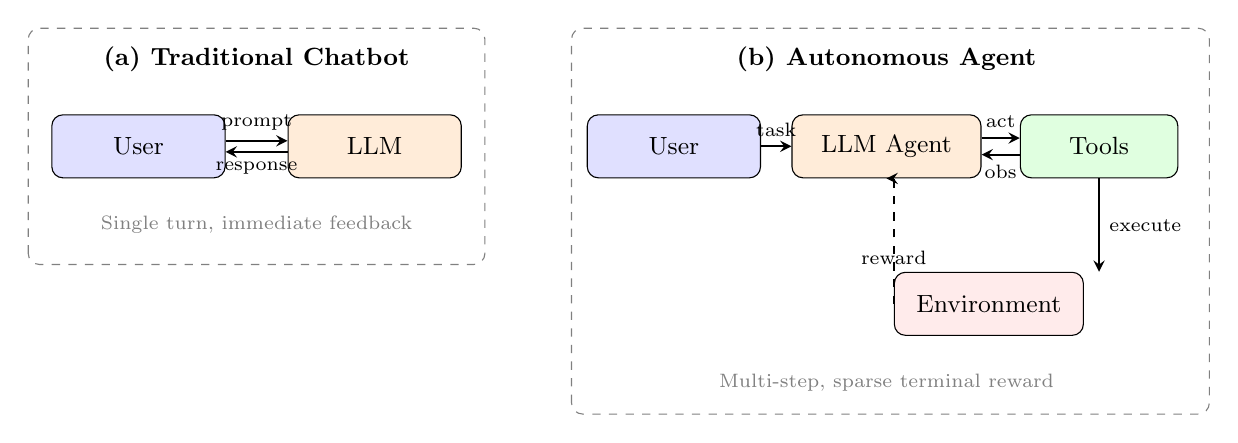
\begin{tikzpicture}[
  box/.style={draw, rounded corners, minimum width=2.2cm, minimum height=0.8cm, font=\small},
  arrow/.style={->, thick, >=stealth},
  lbl/.style={font=\scriptsize, midway, above},
  lblb/.style={font=\scriptsize, midway, below},
]
% --- (a) Chatbot ---
\node[font=\small\bfseries] at (-3.5, 2.6) {(a) Traditional Chatbot};
\node[box, fill=blue!12] (user1) at (-5, 1.5) {User};
\node[box, fill=orange!15] (llm1) at (-2, 1.5) {LLM};
\draw[arrow] ([yshift=2pt]user1.east) -- node[lbl]{prompt} ([yshift=2pt]llm1.west);
\draw[arrow] ([yshift=-2pt]llm1.west) -- node[lblb]{response} ([yshift=-2pt]user1.east);
\node[font=\scriptsize, text=gray] at (-3.5, 0.5) {Single turn, immediate feedback};
\draw[dashed, gray, rounded corners] (-6.4, 0.0) rectangle (-0.6, 3.0);

% --- (b) Autonomous Agent ---
\node[font=\small\bfseries] at (4.5, 2.6) {(b) Autonomous Agent};
\node[box, fill=blue!12] (user2) at (1.8, 1.5) {User};
\node[box, fill=orange!15, minimum width=2.4cm] (agent) at (4.5, 1.5) {LLM Agent};
\node[box, fill=green!12, minimum width=2cm] (tools) at (7.2, 1.5) {Tools};
\node[box, fill=red!8, minimum width=2.4cm] (env) at (5.8, -0.5) {Environment};

% User -> Agent
\draw[arrow] (user2.east) -- node[lbl]{task} (agent.west);
% Agent <-> Tools (bidirectional = the loop)
\draw[arrow] ([yshift=3pt]agent.east) -- node[lbl]{act} ([yshift=3pt]tools.west);
\draw[arrow] ([yshift=-3pt]tools.west) -- node[lblb]{obs} ([yshift=-3pt]agent.east);
% Tools -> Environment
\draw[arrow] (tools.south) -- node[lbl, right]{execute} (tools.south |- env.north);
% Environment -> Agent (reward)
\draw[arrow, dashed] (env.west) -- node[lblb]{reward} (agent.south -| env.west) -- (agent.south);

\node[font=\scriptsize, text=gray] at (4.5, -1.5) {Multi-step, sparse terminal reward};
\draw[dashed, gray, rounded corners] (0.5, -1.9) rectangle (8.6, 3.0);
\end{tikzpicture}
% \caption{From Chatbots to Autonomous Agents: Traditional LLM chatbots operate in a single-step conversational loop with immediate human feedback. Autonomous agents plan across multiple tool interactions, receive feedback from real-world execution environments, and optimize for sparse terminal rewards (task success/failure).}
\caption{从聊天机器人到自主智能体：传统的 LLM 聊天机器人在带有即时人类反馈的单步对话循环中运行。自主智能体跨多个工具交互进行规划，从真实世界的执行环境中接收反馈，并针对稀疏的终端 reward（任务成功/失败）进行优化。}
\end{figure}

% The key differences that demand new RL approaches:
要求新 RL 方法的关键差异：

\begin{itemize}
  % \item \textbf{Multi-step reasoning}: Agents must plan across 10--100+ tool calls, not just generate a single response.
  \item \textbf{多步推理}：Agent 必须跨越 10--100+ 次工具调用进行规划，而不仅仅是生成单一响应。
  % \item \textbf{External environment feedback}: Rewards come from real-world execution (test suites pass, web pages load, code compiles) --- not just human preference scores.
  \item \textbf{外部环境反馈}：Reward 来自真实世界的执行（测试套件通过、网页加载、代码编译），而不仅仅是人类偏好分数。
  % \item \textbf{Structured actions}: Actions are not just tokens but structured outputs (JSON tool calls, API payloads, code blocks).
  \item \textbf{结构化动作}：动作不仅是 Token，而是结构化输出（JSON 工具调用、API 负载、代码块）。
  % \item \textbf{Long horizons with sparse rewards}: Success/failure may only be determined after many intermediate steps.
  \item \textbf{长视野与稀疏 reward}：成功/失败可能只能在多个中间步骤之后才能确定。
\end{itemize}

\begin{intuitionbox}[为什么标准 RLHF 对 Agent 不够用]
% Standard RLHF (PPO/DPO) optimizes for single-turn quality: given a prompt, produce a good response. But agents must:
标准 RLHF（PPO/DPO）针对单轮质量进行优化：给定一个 Prompt，产生一个好的响应。但 Agent 必须：

\begin{itemize}
  % \item Decide \emph{when} to use tools vs. reason internally
  \item 决定\emph{何时}使用工具，还是进行内部推理
  % \item Recover from errors mid-trajectory (self-correction)
  \item 在轨迹中途从错误中恢复（自我纠正）
  % \item Balance exploration (try new approaches) with exploitation (use known-good patterns)
  \item 平衡探索（尝试新方法）与利用（使用已知良好模式）
  % \item Handle partial observability (tool outputs may be incomplete or noisy)
  \item 处理部分可观测性（工具输出可能不完整或带噪声）
\end{itemize}

% This requires training methods that reason over \textbf{entire trajectories}, not individual turns.
这要求训练方法在\textbf{完整轨迹}上进行推理，而不是单个轮次。
\end{intuitionbox}

\section{LLM Agent 的轨迹缓冲区}
\label{trajectory-buffers-for-llm-agents}

% In the context of LLM agents, traditional RL replay buffers undergo a structural transformation. Instead of storing low-dimensional numerical tensors, agentic buffers --- often called \textbf{Trajectory Buffers}, \textbf{Experience Pools}, or \textbf{Memory Banks} --- manage complex textual histories, tool execution outputs, and explicit reasoning steps.
在 LLM Agent 的语境下，传统的 RL 回放缓冲区经历了结构性的转变。Agent 缓冲区——通常称为\textbf{轨迹缓冲区（Trajectory Buffers）}、\textbf{经验池（Experience Pools）}或\textbf{记忆库（Memory Banks）}——不再存储低维数值 Tensor，而是管理复杂的文本历史、工具执行输出和显式推理步骤。

\subsection{LLM Agent 缓冲区的数学结构}
\label{mathematical-structure-of-an-llm-agent-buffer}

% In classic RL, a replay buffer stores a flat tuple $(s, a, r, s')$. For an LLM agent, this expands into high-dimensional tokenized text structures:
在经典 RL 中，回放缓冲区存储扁平元组 $(s, a, r, s')$。对于 LLM Agent，这扩展为高维的 Token 化文本结构：

\begin{equation}
\boxed{e_t = \left( \mathcal{S}_t,\; \mathcal{A}_t,\; \mathcal{R}_t,\; \mathcal{S}_{t+1} \right)}
\end{equation}

\begin{itemize}
  % \item $\mathcal{S}_t$: The \textbf{complete context state} --- system prompt, user objective, conversation history, and current environmental variables (e.g., HTML source code, directory structures, database schemas).
  \item $\mathcal{S}_t$：\textbf{完整上下文状态}——系统 Prompt、用户目标、对话历史，以及当前环境变量（例如 HTML 源代码、目录结构、数据库 Schema）。
  % \item $\mathcal{A}_t$: The agent's \textbf{generated output}, typically composed of a Chain-of-Thought (CoT) reasoning string followed by a structured tool call:
  \item $\mathcal{A}_t$：Agent 的\textbf{生成输出}，通常由一段思维链（Chain-of-Thought，CoT）推理字符串紧接一个结构化工具调用组成：
\begin{equation}
\mathcal{A}_t = \{\text{text}_{\text{reasoning}},\; \text{json}_{\text{tool\_call}}\}
\end{equation}
  % \item $\mathcal{R}_t$: \textbf{Evaluation signals} derived from external execution environments (unit test passes, compiler flags, API response codes) or verified by an LLM-as-a-judge system.
  \item $\mathcal{R}_t$：\textbf{评估信号}，来自外部执行环境（单元测试通过、编译器标志、API 响应码），或由 LLM-as-a-judge 系统验证。
  % \item $\mathcal{S}_{t+1}$: The \textbf{updated context window}, which appends tool output text or error logs directly into the conversation history.
  \item $\mathcal{S}_{t+1}$：\textbf{更新后的上下文窗口}，将工具输出文本或错误日志直接附加到对话历史中。
\end{itemize}

\begin{examplebox}[具体 Agent 轨迹：代码调试]
% \textbf{Step 1}: $\mathcal{S}_1$ = ``Fix the failing test in \texttt{utils.py}''\\
\textbf{步骤 1}：$\mathcal{S}_1$ = ``修复 \texttt{utils.py} 中失败的测试''\\

% $\mathcal{A}_1$ = \emph{``Let me read the file first''} + \texttt{read\_file("utils.py")}\\
$\mathcal{A}_1$ = \emph{``让我先读取该文件''} + \texttt{read\_file("utils.py")}\\

% $\mathcal{R}_1$ = 0 (intermediate step)\\
$\mathcal{R}_1$ = 0（中间步骤）\\

% \textbf{Step 2}: $\mathcal{S}_2$ = [previous context + file contents]\\
\textbf{步骤 2}：$\mathcal{S}_2$ = [先前上下文 + 文件内容]\\

% $\mathcal{A}_2$ = \emph{``The bug is on line 42, off-by-one error''} + \texttt{edit\_file("utils.py", ...)}\\
$\mathcal{A}_2$ = \emph{``Bug 在第 42 行，是一个差一错误''} + \texttt{edit\_file("utils.py", ...)}\\

% $\mathcal{R}_2$ = 0 (intermediate step)\\
$\mathcal{R}_2$ = 0（中间步骤）\\

% \textbf{Step 3}: $\mathcal{S}_3$ = [previous context + edit confirmation]\\
\textbf{步骤 3}：$\mathcal{S}_3$ = [先前上下文 + 编辑确认]\\

% $\mathcal{A}_3$ = \emph{``Let me verify the fix''} + \texttt{run\_tests()}\\
$\mathcal{A}_3$ = \emph{``让我验证修复''} + \texttt{run\_tests()}\\

% $\mathcal{R}_3$ = +1.0 (all tests pass --- sparse terminal reward)
$\mathcal{R}_3$ = +1.0（所有测试通过——稀疏终端 reward）
\end{examplebox}

\section{操作范式}
\label{operational-paradigms}

% LLM agents leverage specialized trajectory buffers through three primary optimization methodologies:
LLM Agent 通过三种主要的优化方法论来利用专门的轨迹缓冲区：

\subsection{A. 自我纠正与思维细化}
\label{a.-self-correction-and-thought-refinement-star-reflexion}

% Two representative methods in this category are STaR \cite{zelikman2022star} and Reflexion \cite{shinn2023reflexion}. When an agent fails a multi-step execution trace, the sub-optimal sequence is saved to the buffer. The framework later samples this trajectory and prompts the LLM to generate an explicit textual critique of its past performance:
此类别中的两种代表性方法是 STaR \cite{zelikman2022star} 和 Reflexion \cite{shinn2023reflexion}。当 Agent 在一次多步执行轨迹中失败时，次优序列会被保存到缓冲区。该框架随后采样此轨迹，并提示 LLM 对其过去的表现生成显式文本批评：
\begin{equation}
\text{Critique} \leftarrow \text{LLM}(\mathcal{S}_{\text{failed}},\; \mathcal{A}_{\text{failed}},\; \mathcal{R}_{=0})
\end{equation}

% Once a corrected trajectory achieves a positive reward, it is moved to an optimal experience pool used to update the network weights via fine-tuning (SFT on successful trajectories) or RL (GRPO~\cite{shao2024deepseekmath} with binary pass/fail rewards).
一旦修正后的轨迹获得正向 reward，它就被移至最优经验池，用于通过微调（在成功轨迹上做 SFT）或 RL（采用二元通过/失败 reward 的 GRPO~\cite{shao2024deepseekmath}）来更新网络权重。

\begin{keybox}[STaR：自学习推理者]
\begin{enumerate}
  % \item Generate reasoning traces for a batch of problems
  \item 为一批问题生成推理轨迹
  % \item Filter: keep only traces that lead to correct answers
  \item 过滤：仅保留导致正确答案的轨迹
  % \item Fine-tune the model on successful traces (SFT)
  \item 在成功轨迹上微调模型（SFT）
  % \item Repeat: the improved model generates better traces in the next iteration
  \item 重复：改进后的模型在下一次迭代中生成更好的轨迹
\end{enumerate}

% Each iteration bootstraps the model's reasoning ability using its own successful outputs as training data.
每次迭代都使用模型自身的成功输出作为训练数据，自举其推理能力。
\end{keybox}

\begin{keybox}[Reflexion：语言强化学习]
\begin{enumerate}
  % \item Agent attempts a task, fails
  \item Agent 尝试一项任务，失败
  % \item Agent generates a \textbf{verbal reflection}: ``I failed because I didn't check the return type before calling the API''
  \item Agent 生成一段\textbf{语言反思}：``我失败是因为在调用 API 之前没有检查返回类型''
  % \item Reflection is stored in an episodic memory buffer
  \item 反思被存储在一个情节记忆缓冲区中
  % \item On the next attempt, reflections are injected into the prompt as lessons learned
  \item 在下一次尝试中，反思作为经验教训被注入到 Prompt 中
  % \item No weight updates needed --- pure in-context learning from self-critique
  \item 不需要权重更新——纯粹通过自我批评进行上下文学习
\end{enumerate}
\end{keybox}

\subsection{B. 离策略探索}
\label{b.-off-policy-exploration-react-tool-use-frameworks}

% This paradigm, exemplified by ReAct \cite{yao2023react} and related tool-use frameworks, involves extensive autonomous exploration. During autonomous exploration (web navigation, database querying, code generation), agents log thousands of exploratory execution paths. The trajectory buffer acts as a filter:
此范式以 ReAct \cite{yao2023react} 及相关工具使用框架为代表，涉及广泛的自主探索。在自主探索过程中（网页导航、数据库查询、代码生成），Agent 记录数千条探索性执行路径。轨迹缓冲区充当一个过滤器：

\begin{itemize}
  % \item \textbf{Success filtering}: Only trajectories achieving the goal are kept for training.
  \item \textbf{成功过滤}：只保留达成目标的轨迹用于训练。
  % \item \textbf{Efficiency ranking}: Among successful traces, prefer the shortest/most efficient tool-use paths.
  \item \textbf{效率排序}：在成功轨迹中，优先选择最短/最高效的工具使用路径。
  % \item \textbf{Diversity sampling}: Maintain a diverse set of solution strategies to prevent mode collapse.
  \item \textbf{多样性采样}：维持多样化的解决策略集合，以防止模式坍塌。
\end{itemize}

% The optimization algorithm (typically GRPO~\cite{shao2024deepseekmath} or filtered SFT) computes losses exclusively over efficient, successful trajectories while discarding meandering runs.
优化算法（通常是 GRPO~\cite{shao2024deepseekmath} 或过滤后的 SFT）只在高效、成功的轨迹上计算 Loss，丢弃迂回曲折的运行。

\subsection{C. 非参数化的上下文学习（基于经验的 RAG）}
\label{c.-non-parametric-in-context-learning-rag-over-experiences}

% Instead of modifying neural network weights, the trajectory buffer can function as a \textbf{vector database}. Given a new user goal $\mathcal{G}_{\text{new}}$, the system retrieves the most relevant past experiences:
轨迹缓冲区可以不修改神经网络权重，而是作为一个\textbf{向量数据库}。给定一个新的用户目标 $\mathcal{G}_{\text{new}}$，系统检索最相关的过往经验：
\begin{equation}
\boxed{\mathcal{E}_{\text{retrieved}} = \arg\max_{e \in \mathcal{B}} \text{sim}\!\left(\text{Embed}(\mathcal{G}_{\text{new}}),\; \text{Embed}(e)\right)}
\end{equation}

% The top-$k$ similar successful historical runs are injected directly into the prompt context as few-shot demonstrations. This approach:
Top-$k$ 个相似的成功历史运行作为 few-shot 示例直接注入到 Prompt 上下文中。这种方法：

\begin{itemize}
  % \item Requires \textbf{zero training} --- pure retrieval-augmented generation
  \item 需要\textbf{零训练}——纯粹的检索增强生成（Retrieval-Augmented Generation, RAG）
  % \item Adapts instantly to new tasks if similar experiences exist in the buffer
  \item 如果缓冲区中存在相似经验，可即时适应新任务
  % \item Scales with buffer size (more experiences = better coverage)
  \item 随缓冲区规模扩展（更多经验 = 更好的覆盖率）
  % \item Complements parametric learning (use retrieval for rare cases, weights for common patterns)
  \item 与参数化学习互补（罕见情况使用检索，常见模式使用权重）
\end{itemize}

\section{范式对比}
\label{paradigm-comparison}

\begin{table}[ht!]
\centering\small
% \caption{Traditional RL Buffers vs. LLM Agent Buffers}
\caption{传统 RL 缓冲区与 LLM Agent 缓冲区对比}
\begin{tabularx}{0.88\linewidth}{@{}l Z{0.77} Z{1.23}@{}}
\toprule
\textbf{特性} & \textbf{传统 RL 缓冲区} & \textbf{LLM Agent 缓冲区} \\
\midrule
\textbf{数据格式} & 连续向量 / Tensor & Token 化文本、JSON、代码块、工具输出 \\
\textbf{数据量} & 海量（$10^5$--$10^7$ 条） & 中小规模（$10^3$--$10^5$ 条轨迹） \\
\textbf{主要目标} & 打破数据相关性 & 提供推理示范 \\
\textbf{采样} & 随机均匀 / PER & 语义检索 / 成功优先 / 多样性 \\
\textbf{状态大小} & 固定（如 84$\times$84 像素） & 可变（每个状态 1K--128K Token） \\
\textbf{动作空间} & 离散/连续向量 & 结构化文本（推理 + 工具调用） \\
\textbf{Reward 来源} & 环境模拟器 & 外部执行 / LLM judge / 单元测试 \\
\bottomrule
\end{tabularx}
\end{table}

\section{Agent RL 的主要技术}
\label{major-techniques-in-agentic-rl}

\begin{table}[ht!]
\centering\small
% \caption{Key methods for training LLM agents with RL.}
\caption{用 RL 训练 LLM Agent 的关键方法。}
\noindent\begin{tabularx}{\linewidth}{@{}l l Z{1}@{}}
\toprule
\textbf{方法} & \textbf{类型} & \textbf{核心思想} \\
\midrule
\textbf{STaR}~\cite{zelikman2022star} & 迭代 SFT & 通过在自身成功轨迹上微调来自举推理能力 \\
\textbf{Reflexion}~\cite{shinn2023reflexion} & 上下文 RL & 语言式自我批评作为情节记忆存储；无权重更新 \\
\textbf{ReAct}~\cite{yao2023react} & Prompt 方法 & 在单次生成中交错推理（``思考''）与行动（``工具调用''） \\
\textbf{LATS}~\cite{zhou2024lats} & 树搜索 & 在动作序列上做蒙特卡洛树搜索；反向传播 reward \\
\textbf{AgentQ}~\cite{putta2024agentq} & 离策略 RL & 在 Agent 轨迹上用 AI 生成的偏好对做 DPO \\
\textbf{OpenHands}~\cite{wang2024openhands} & GRPO & 基于执行的 reward（测试通过/失败）做组相对优化 \\
\textbf{Voyager}~\cite{wang2023voyager} & 技能库 & 存储并检索成功代码片段以组合复用 \\
\textbf{RLEF}~\cite{le2024rlef} & 在线 RL & 从执行反馈中做 RL——来自代码/测试执行的二元 reward \\
\bottomrule
\end{tabularx}
\end{table}

\subsection{STaR：自学习推理者（详解）}
\label{star-self-taught-reasoner-detailed}

% STaR~\cite{zelikman2022star} is an \textbf{iterative self-improvement} method that bootstraps reasoning capabilities without external reward models. The core insight: if the model can occasionally solve a problem correctly, it can learn from its own successes.
STaR~\cite{zelikman2022star} 是一种\textbf{迭代式自我改进}方法，无需外部 Reward Model 即可自举推理能力。核心洞见：如果模型偶尔能正确解决一个问题，它就可以从自身的成功中学习。

% \textbf{Algorithm}:
\textbf{算法}：

\begin{enumerate}
  % \item \textbf{Generate}: For each problem $x_i$ in dataset $\mathcal{D}$, sample a reasoning trace $z_i \sim \pi_\theta(\cdot | x_i)$ followed by an answer $\hat{y}_i$.
  \item \textbf{生成}：对数据集 $\mathcal{D}$ 中的每个问题 $x_i$，采样一条推理轨迹 $z_i \sim \pi_\theta(\cdot | x_i)$，后跟一个答案 $\hat{y}_i$。
  % \item \textbf{Filter}: Keep only traces where $\hat{y}_i = y_i^*$ (correct answer). Define success set $\mathcal{D}_{\text{pass}} = \{(x_i, z_i, y_i^*) : \hat{y}_i = y_i^*\}$.
  \item \textbf{过滤}：仅保留满足 $\hat{y}_i = y_i^*$（正确答案）的轨迹。定义成功集 $\mathcal{D}_{\text{pass}} = \{(x_i, z_i, y_i^*) : \hat{y}_i = y_i^*\}$。
  % \item \textbf{Rationalization} (key innovation): For problems where the model failed, generate a ``rationalization'' --- a trace conditioned on the correct answer: $z_i^{\text{rat}} \sim \pi_\theta(\cdot | x_i, y_i^*)$. This teaches the model to reason \emph{backward} from solutions.
  \item \textbf{合理化（Rationalization）}（关键创新）：对模型失败的问题，生成一条以正确答案为条件的``合理化''轨迹：$z_i^{\text{rat}} \sim \pi_\theta(\cdot | x_i, y_i^*)$。这教导模型从解\emph{反向}推理。
  % \item \textbf{Fine-tune}: Update $\theta$ via SFT on $\mathcal{D}_{\text{pass}} \cup \mathcal{D}_{\text{rationalized}}$.
  \item \textbf{微调}：在 $\mathcal{D}_{\text{pass}} \cup \mathcal{D}_{\text{rationalized}}$ 上通过 SFT 更新 $\theta$。
  % \item \textbf{Iterate}: Repeat from step 1 with the improved model.
  \item \textbf{迭代}：用改进后的模型从步骤 1 重复。
\end{enumerate}

\begin{equation}
\boxed{\theta_{k+1} = \arg\min_\theta -\sum_{(x,z,y) \in \mathcal{D}_k^+} \log \pi_\theta(z, y | x)}
\end{equation}

% \textbf{Convergence dynamics}: Each iteration $k$ increases the model's solve rate $p_k$. If $p_0 = 0.3$ (solves 30\% of problems), after rationalization + SFT, $p_1 \approx 0.5$. Typically converges in 3--5 iterations to $p \approx 0.7$--$0.9$.
\textbf{收敛动力学}：每次迭代 $k$ 都会提升模型的解题率 $p_k$。若 $p_0 = 0.3$（解出 30\% 的问题），经过合理化 + SFT 后 $p_1 \approx 0.5$。通常 3--5 次迭代后收敛至 $p \approx 0.7$--$0.9$。

\begin{examplebox}[STaR 合理化 Prompt]
\begin{lstlisting}[style=pythonstyle]
# 标准生成（步骤 1）：
PROMPT = """Solve the following problem step by step.
Problem: A store has 45 apples. It sells 3/5 of them. How many remain?
Let's think step by step:"""

# 合理化 Prompt（步骤 3——以正确答案为条件）：
PROMPT_RATIONALIZE = """Solve the following problem step by step.
The correct answer is 18.
Problem: A store has 45 apples. It sells 3/5 of them. How many remain?
Let's think step by step to arrive at 18:"""

# Agent 变体（带错误条件的代码任务）：
PROMPT_AGENT_RATIONALIZE = """The following code task failed with the error below.
Generate a correct solution step by step.

Task: Implement binary search that handles duplicates.
Previous error: IndexError: list index out of range (line 12)
Correct behavior: Return leftmost index of target.

Let me fix this by reasoning about the boundary conditions:"""
\end{lstlisting}
\end{examplebox}

\begin{intuitionbox}[面向 Agent 的 STaR 变体]
\begin{itemize}
  % \item \textbf{Quiet-STaR}~\cite{zelikman2024quietstar}: Inserts ``thinking tokens'' between every token of generation. The model learns to reason \emph{implicitly} without explicit CoT prompting. Training objective: predict next tokens better when thinking tokens are included.
  \item \textbf{Quiet-STaR}~\cite{zelikman2024quietstar}：在每个生成 Token 之间插入``思考 Token''。模型学会在没有显式 CoT 提示的情况下\emph{隐式}推理。训练目标：在包含思考 Token 时更好地预测下一个 Token。
  % \item \textbf{STaR for Code Agents}: Replace answer verification with test execution. ``Correct'' = all tests pass. Rationalization = generate a new approach conditioned on the error message.
  \item \textbf{代码 Agent 的 STaR}：用测试执行替代答案验证。``正确'' = 所有测试通过。合理化 = 以错误消息为条件生成新方法。
  % \item \textbf{V-STaR}~\cite{hosseini2024vstar}: Adds a verifier model trained on $(z, y, \text{correct/incorrect})$ triples. The verifier provides process-level supervision, filtering bad reasoning traces that accidentally reach correct answers.
  \item \textbf{V-STaR}~\cite{hosseini2024vstar}：增加一个在 $(z, y, \text{correct/incorrect})$ 三元组上训练的验证器模型。该验证器提供过程级监督，过滤那些偶然到达正确答案的糟糕推理轨迹。
\end{itemize}
\end{intuitionbox}

\subsection{Reflexion：语言强化学习（详解）}
\label{reflexion-verbal-reinforcement-learning-detailed}

% Reflexion~\cite{shinn2023reflexion} introduces a radical paradigm: \textbf{RL without weight updates}. Instead of gradient-based learning, the agent improves through natural-language self-critique stored in an episodic memory.
Reflexion~\cite{shinn2023reflexion} 引入了一种激进的范式：\textbf{无权重更新的 RL}。Agent 不通过基于梯度的学习，而是通过存储在情节记忆中的自然语言自我批评来改进。

% \textbf{Full Architecture}:
\textbf{完整架构}：

\begin{enumerate}
  % \item \textbf{Actor}: The LLM agent $\pi$ that executes actions in the environment.
  \item \textbf{Actor}：在环境中执行动作的 LLM Agent $\pi$。
  % \item \textbf{Evaluator}: A binary signal (task success/failure) or a scalar heuristic (e.g., number of test cases passed).
  \item \textbf{评估器}：二元信号（任务成功/失败）或标量启发式（如通过的测试用例数）。
  % \item \textbf{Self-Reflection Generator}: Given the failed trajectory $\tau_{\text{fail}}$ and environment feedback, generates a natural-language reflection $r_{\text{text}}$:
  \item \textbf{自我反思生成器}：给定失败轨迹 $\tau_{\text{fail}}$ 和环境反馈，生成自然语言反思 $r_{\text{text}}$：
\begin{equation}
r_{\text{text}} = \text{LLM}_{\text{reflect}}\!\left(\tau_{\text{fail}}, \text{feedback}, \text{task}\right)
\end{equation}
  % \item \textbf{Episodic Memory}: A sliding window buffer $\mathcal{M} = [r_1, r_2, \ldots, r_m]$ of past reflections (typically $m \leq 3$ to fit in context).
  \item \textbf{情节记忆}：过往反思的滑动窗口缓冲区 $\mathcal{M} = [r_1, r_2, \ldots, r_m]$（通常 $m \leq 3$ 以适应上下文）。
  % \item \textbf{Retry Loop}: On the next attempt, reflections are injected into the prompt:
  \item \textbf{重试循环}：下一次尝试时，反思被注入到 Prompt 中：
\begin{equation}
a_{t+1} \sim \pi\!\left(\cdot\; |\; \text{task},\; \mathcal{M},\; \text{current\_state}\right)
\end{equation}
\end{enumerate}

% \textbf{Example reflection}: \emph{``In my previous attempt, I called the search API before validating the input format, which caused a 400 error. Next time, I should validate the JSON schema first, then make the API call.''}
\textbf{反思示例}：\emph{``在我上一次尝试中，我在验证输入格式之前就调用了搜索 API，导致了 400 错误。下次我应该先验证 JSON Schema，然后再发起 API 调用。''}

\begin{examplebox}[Reflexion：带记忆注入的 Agent Prompt]
\begin{lstlisting}[style=pythonstyle]
# === 第 2 次尝试的 PROMPT（首次失败后）===

SYSTEM = """You are a coding agent. You can run bash commands and edit files.
Complete the task below. Learn from your previous reflections."""

USER = """Task: Fix the failing test in auth_service.py

=== REFLECTIONS FROM PREVIOUS ATTEMPTS ===
[Attempt 1 reflection]: I tried to modify the authenticate() function
directly but forgot that it depends on token_validator(). The test
failed because token_validator() was still returning the old format.
I should trace the dependency chain FIRST: check what authenticate()
calls, then fix the root cause (token_validator), not the symptom.
=== END REFLECTIONS ===

The repository is in /workspace/. The failing test is:
  test_auth.py::test_expired_token_returns_401

Begin by reading the relevant files, then fix the issue."""
\end{lstlisting}
\end{examplebox}

% \textbf{Strengths and Limitations}:
\textbf{优势与局限}：

{\small
\noindent\begin{tabularx}{\linewidth}{@{}Z{1.03} Z{0.97}@{}}
\toprule
\textbf{优势} & \textbf{局限} \\
\midrule
零梯度计算；可与冻结的 API 模型（GPT-4）一起工作 & 受限于上下文窗口；无法积累无限知识 \\
快速迭代（每次重试只需几秒，而 RL 训练需数小时） & 无法泛化到未见任务（记忆是任务特定的） \\
可解释：人类可读的自我纠正 & 依赖模型已有的识别错误的能力 \\
可与任意基础 Agent 架构组合 & 当基础模型太弱、无法生成有用批评时，效果下降 \\
\bottomrule
\end{tabularx}
}

\subsection{ReAct：推理 + 行动（详解）}
\label{react-reasoning-acting-detailed}

% ReAct~\cite{yao2023react} establishes the dominant prompting paradigm for tool-using agents by \textbf{interleaving explicit reasoning steps with environment actions} in a single generation stream.
ReAct~\cite{yao2023react} 通过在单个生成流中\textbf{交错显式推理步骤与环境动作}，确立了工具使用 Agent 的主导 Prompt 范式。

\begin{examplebox}[ReAct 系统 Prompt（典型）]
\begin{lstlisting}[style=pythonstyle]
SYSTEM = """You are a research assistant with access to the following tools:
- search(query): Search the web for information
- lookup(term): Look up a term on the current Wikipedia page
- finish(answer): Submit your final answer

Solve the user's question by interleaving Thought and Action steps.
Format:
  Thought: <your reasoning about what to do next>
  Action: <tool_name>(arguments)

You will receive an Observation after each Action. Use it to plan
your next step. Continue until you can provide a final answer.

Rules:
- Always think before acting
- Never guess - verify with tools
- Use finish() only when you are confident in your answer"""

USER = "Who was the president of the US when the iPhone was released?"
\end{lstlisting}
\end{examplebox}

% \textbf{Generation format}:
\textbf{生成格式}：

\begin{examplebox}[ReAct 轨迹格式]
\begin{lstlisting}[style=pythonstyle]
Thought: I need to find when the iPhone was released, then determine
who was president at that time. Let me search for the release date.
Action: search("iPhone original release date")
Observation: The original iPhone was released on June 29, 2007.
Thought: The iPhone came out June 2007. Now I need to find who was
the US president in June 2007.
Action: lookup("President of the United States in 2007")
Observation: George W. Bush served as the 43rd president from
January 20, 2001 to January 20, 2009.
Thought: George W. Bush was president from 2001-2009, which covers
June 2007 when the iPhone was released. I have my answer.
Action: finish("George W. Bush was the US president when the iPhone
was released on June 29, 2007.")
\end{lstlisting}
\end{examplebox}

% \textbf{Formal definition}: A ReAct trajectory is $\tau = (t_1, a_1, o_1, t_2, a_2, o_2, \ldots)$ where:
\textbf{形式化定义}：一条 ReAct 轨迹是 $\tau = (t_1, a_1, o_1, t_2, a_2, o_2, \ldots)$，其中：

\begin{itemize}
  % \item $t_i$: Thought (internal reasoning, not executed)
  \item $t_i$：思考（内部推理，不被执行）
  % \item $a_i$: Action (tool call, executed in environment)
  \item $a_i$：动作（工具调用，在环境中执行）
  % \item $o_i$: Observation (environment response, appended to context)
  \item $o_i$：观测（环境响应，附加到上下文）
\end{itemize}

% \textbf{Why it works}: Thoughts create an ``inner monologue'' that helps the model plan before acting, reducing impulsive tool calls. The explicit reasoning trace also makes the agent's decision process \textbf{auditable} and \textbf{debuggable}.
\textbf{为什么有效}：思考创造了一种``内心独白''，帮助模型在行动前规划，减少冲动性工具调用。显式推理轨迹也让 Agent 的决策过程\textbf{可审计}且\textbf{可调试}。

% \textbf{Training ReAct agents with RL}:
\textbf{用 RL 训练 ReAct Agent}：

\begin{itemize}
  % \item \textbf{Action-level rewards}: Only actions receive reward signals (thoughts are auxiliary).
  \item \textbf{动作级 reward}：只有动作接收 reward 信号（思考是辅助的）。
  % \item \textbf{Thought quality}: Implicitly optimized --- better thoughts $\rightarrow$ better actions $\rightarrow$ higher rewards.
  \item \textbf{思考质量}：隐式优化——更好的思考 $\rightarrow$ 更好的动作 $\rightarrow$ 更高的 reward。
  % \item \textbf{Format enforcement}: Include format penalties in the reward for malformed actions (missing JSON, hallucinated tools).
  \item \textbf{格式强制}：在 reward 中加入对格式错误动作（缺失 JSON、幻觉工具）的格式惩罚。
  % \item \textbf{RL objective}: $r(\tau) = r_{\text{task}} - \lambda_{\text{format}} \cdot \text{format\_violations} - \lambda_{\text{length}} \cdot \text{num\_steps}$
  \item \textbf{RL 目标}：$r(\tau) = r_{\text{task}} - \lambda_{\text{format}} \cdot \text{format\_violations} - \lambda_{\text{length}} \cdot \text{num\_steps}$
\end{itemize}

\subsection{LATS：语言 Agent 树搜索（详解）}
\label{lats-language-agent-tree-search-detailed}

% LATS~\cite{zhou2024lats} applies \textbf{Monte Carlo Tree Search (MCTS)} to LLM agent action selection, trading inference compute for significantly better trajectories.
LATS~\cite{zhou2024lats} 将\textbf{蒙特卡洛树搜索（Monte Carlo Tree Search, MCTS）}应用于 LLM Agent 的动作选择，以推理算力换取显著更好的轨迹。

% \textbf{Algorithm (adapted for LLM agents)}:
\textbf{算法（针对 LLM Agent 改造）}：

\begin{enumerate}
  % \item \textbf{Selection}: Starting from root (initial state), traverse the tree using UCB1:
  \item \textbf{选择}：从根节点（初始状态）开始，使用 UCB1 遍历树：
\begin{equation}
\text{UCB}(s, a) = \bar{Q}(s, a) + c \sqrt{\frac{\ln N(s)}{N(s, a)}}
\end{equation}
 % where $\bar{Q}$ = average reward of subtree, $N$ = visit counts, $c$ = exploration constant.
 其中 $\bar{Q}$ = 子树平均 reward，$N$ = 访问计数，$c$ = 探索常数。
  % \item \textbf{Expansion}: At a leaf node, generate $k$ candidate actions via LLM sampling (temperature $> 0$): $\{a_1, \ldots, a_k\} \sim \pi_\theta(\cdot | s_{\text{leaf}})$
  \item \textbf{扩展}：在叶节点，通过 LLM 采样（温度 $> 0$）生成 $k$ 个候选动作：$\{a_1, \ldots, a_k\} \sim \pi_\theta(\cdot | s_{\text{leaf}})$
  % \item \textbf{Simulation}: For each candidate, execute the action in the environment and continue with a fast rollout policy (greedy decoding) until terminal state or depth limit.
  \item \textbf{模拟}：对每个候选，在环境中执行该动作，然后用快速 rollout 策略（贪心解码）继续，直到终止状态或深度限制。
  % \item \textbf{Backpropagation}: Propagate the terminal reward up through all ancestor nodes, updating $\bar{Q}$ and $N$ counts.
  \item \textbf{反向传播}：将终端 reward 沿所有祖先节点向上传播，更新 $\bar{Q}$ 和 $N$ 计数。
  % \item \textbf{Repeat}: Run steps 1--4 for a fixed computation budget (e.g., 50--200 iterations).
  \item \textbf{重复}：在固定计算预算（如 50--200 次迭代）下运行步骤 1--4。
  % \item \textbf{Action selection}: Choose the most-visited child of the root.
  \item \textbf{动作选择}：选择根节点访问次数最多的子节点。
\end{enumerate}

% \textbf{LLM-specific adaptations}:
\textbf{LLM 特定的改造}：

\begin{itemize}
  % \item \textbf{Value function}: Use a separate LLM call to estimate state value: ``On a scale of 0--1, how likely is this state to lead to task success?''
  \item \textbf{Value 函数}：使用独立的 LLM 调用来估计状态价值：``在 0--1 范围内，这个状态导致任务成功的可能性有多大？''
  % \item \textbf{Reflection-based pruning}: When a branch fails, generate a reflection and prune similar branches.
  \item \textbf{基于反思的剪枝}：当某个分支失败时，生成反思并剪枝相似分支。
  % \item \textbf{Caching}: Store LLM outputs at each node to avoid redundant generation during backtracking.
  \item \textbf{缓存}：在每个节点存储 LLM 输出，避免回溯时重复生成。
  % \item \textbf{Depth budget}: Limit tree depth to 10--20 steps (agents rarely need more).
  \item \textbf{深度预算}：将树深度限制在 10--20 步（Agent 很少需要更多）。
\end{itemize}

% \textbf{Performance}: On WebShop (web navigation), LATS achieves 75\% success vs. ReAct's 40\%. On HumanEval (code), pass@1 improves from 68\% $\rightarrow$ 94\% with tree search. The cost: 10--50$\times$ more inference FLOPs per task.
\textbf{性能}：在 WebShop（网页导航）上，LATS 达到 75\% 成功率，而 ReAct 仅为 40\%。在 HumanEval（代码）上，借助树搜索 pass@1 从 68\% 提升至 94\%。代价：每个任务的推理 FLOPs 增加 10--50$\times$。

\begin{examplebox}[LATS Prompt：价值估计与节点扩展]
\begin{lstlisting}[style=pythonstyle]
# === 价值估计 PROMPT（用于模拟阶段）===
VALUE_PROMPT = """You are evaluating an agent's progress on a task.

Task: Book a flight from NYC to London for under \$500, departing Dec 15.

Current state (after 3 actions):
- Searched flights on Kayak: found 12 results
- Filtered by price < \$500: 4 options remain
- Clicked on British Airways \$489 option: viewing details page

On a scale of 0.0 to 1.0, how likely is the agent to successfully
complete the task from this state? Consider:
- How close is the agent to the goal?
- Are there remaining obstacles (payment, seat selection)?
- Has the agent made any errors that need correction?

Score: """  # 模型输出，例如 "0.75"

# === 节点扩展 PROMPT（生成候选动作）===
EXPAND_PROMPT = """You are a web navigation agent. Given the current
page state, propose 3 DIFFERENT next actions to try.

Current page: British Airways booking - flight details
  Price: \$489 | Departure: Dec 15 8:30am | Arrival: Dec 15 8:45pm
  [Button: Select] [Button: Back to results] [Link: Fare rules]

Generate 3 diverse candidate actions (explore different strategies):
Action 1:"""  # 模型生成 3 个选项用于树扩展
\end{lstlisting}
\end{examplebox}

\subsection{AgentQ：在 Agent 轨迹上做 DPO（详解）}
\label{agentq-dpo-on-agent-trajectories-detailed}

% AgentQ~\cite{putta2024agentq} bridges \textbf{offline preference learning (DPO)} with \textbf{online agent execution} by automatically generating preference pairs from trajectory outcomes.
AgentQ~\cite{putta2024agentq} 通过从轨迹结果自动生成偏好对，桥接了\textbf{离线偏好学习（DPO）}与\textbf{在线 Agent 执行}。

% \textbf{Pipeline}:
\textbf{流水线}：

\begin{enumerate}
  % \item \textbf{Rollout}: Execute $N$ trajectories per task using the current policy $\pi_\theta$.
  \item \textbf{Rollout}：使用当前 Policy $\pi_\theta$ 为每个任务执行 $N$ 条轨迹。
  % \item \textbf{Evaluate}: Score each trajectory with execution-based reward (binary pass/fail or scalar metric).
  \item \textbf{评估}：用基于执行的 reward（二元通过/失败或标量指标）为每条轨迹打分。
  % \item \textbf{Pair construction}: For each task, construct preference pairs:
  \item \textbf{偏好对构造}：对每个任务，构造偏好对：
\begin{equation}
(\tau_w, \tau_l) \text{ where } r(\tau_w) > r(\tau_l)
\end{equation}
 % Among trajectories for the same task, the one with highest reward = chosen; lowest = rejected.
 在同一任务的轨迹中，reward 最高者 = 被选（chosen），最低者 = 被拒（rejected）。
  % \item \textbf{DPO update}: Apply standard DPO loss over trajectory-level log-probabilities:
  \item \textbf{DPO 更新}：在轨迹级对数概率上应用标准 DPO Loss：
\begin{equation}
\mathcal{L}_{\text{AgentQ}} = -\log \sigma\!\left(\beta \left[\log\frac{\pi_\theta(\tau_w)}{\pi_{\text{ref}}(\tau_w)} - \log\frac{\pi_\theta(\tau_l)}{\pi_{\text{ref}}(\tau_l)}\right]\right)
\end{equation}
  % \item \textbf{Iterate}: Updated $\pi_\theta$ generates new (better) trajectories in the next round.
  \item \textbf{迭代}：更新后的 $\pi_\theta$ 在下一轮生成更好的轨迹。
\end{enumerate}

% \textbf{Key design choices}:
\textbf{关键设计选择}：

\begin{itemize}
  % \item \textbf{MCTS-guided exploration}: Use LATS during rollout phase to generate diverse, high-quality trajectories (better training data).
  \item \textbf{MCTS 引导的探索}：在 rollout 阶段使用 LATS 生成多样、高质量的轨迹（更好的训练数据）。
  % \item \textbf{Step-level DPO}: Instead of comparing full trajectories, compare at the \emph{action level} --- given the same prefix, which next action leads to success?
  \item \textbf{步骤级 DPO}：不比较完整轨迹，而是在\emph{动作级别}比较——给定相同前缀，哪个下一动作导向成功？
  % \item \textbf{Self-play improvement}: Each DPO iteration produces a better policy that generates better trajectories that produce better training pairs --- a virtuous cycle.
  \item \textbf{自对弈改进}：每次 DPO 迭代都产生更好的 Policy，生成更好的轨迹，从而产生更好的训练对——一个良性循环。
\end{itemize}

% \textbf{Results}: On WebShop, AgentQ achieves absolute 50\% $\rightarrow$ 82\% success rate improvement over the base policy in 3 DPO iterations.
\textbf{结果}：在 WebShop 上，AgentQ 在 3 次 DPO 迭代后将成功率从 50\% 绝对提升至 82\%。

\subsection{Voyager：通过技能库实现终身学习（详解）}
\label{voyager-lifelong-learning-via-skill-libraries-detailed}

% Voyager~\cite{wang2023voyager} introduces \textbf{compositional skill accumulation} --- the agent builds a growing library of reusable code functions that serve as high-level actions.
Voyager~\cite{wang2023voyager} 引入了\textbf{组合式技能积累}——Agent 构建一个不断增长的可复用代码函数库，作为高层动作。

% \textbf{Architecture}:
\textbf{架构}：

\begin{enumerate}
  % \item \textbf{Automatic Curriculum}: An LLM proposes progressively harder tasks based on the agent's current skill inventory: ``You can now mine wood and craft planks. Next challenge: build a crafting table.''
  \item \textbf{自动课程}：一个 LLM 根据 Agent 当前的技能清单提议逐渐更难的任务：``你现在能挖木头并合成木板。下一个挑战：建造一个工作台。''
  % \item \textbf{Skill Generation}: For each task, the agent writes a JavaScript function (executable code) that solves it:
  \item \textbf{技能生成}：对每个任务，Agent 编写一个 JavaScript 函数（可执行代码）来解决它：
\begin{equation}
\text{skill}_i = \text{LLM}(\text{task}_i, \text{environment\_docs}, \text{error\_feedback})
\end{equation}
  % \item \textbf{Verification}: Execute the code in the environment. If it succeeds, add to the skill library. If not, iterate with error feedback (up to 5 retries).
  \item \textbf{验证}：在环境中执行代码。如果成功，加入技能库。若失败，借助错误反馈迭代（最多 5 次重试）。
  % \item \textbf{Skill Library} (vector DB): Each verified skill stored with:
  \item \textbf{技能库}（向量数据库）：每个已验证技能存储：

\begin{itemize}
  % \item Function signature + docstring (for retrieval)
  \item 函数签名 + Docstring（用于检索）
  % \item Embedding of the task description (for semantic search)
  \item 任务描述的 Embedding（用于语义搜索）
  % \item Dependencies (which other skills it calls)
  \item 依赖（它调用了哪些其他技能）
\end{itemize}
  % \item \textbf{Retrieval + Composition}: For new tasks, retrieve the top-$k$ most relevant skills and compose them:
  \item \textbf{检索 + 组合}：对新任务，检索 top-$k$ 最相关技能并加以组合：
\begin{equation}
\text{solution} = \text{LLM}(\text{new\_task}, \text{retrieve}(\text{skill\_library}, k{=}5))
\end{equation}
\end{enumerate}

% \textbf{Key insight}: Skills are \textbf{compositional} --- complex behaviors emerge from combining simple verified functions. The agent never forgets (library is persistent) and improves monotonically (only verified skills are added).
\textbf{关键洞见}：技能是\textbf{可组合的}——复杂行为从组合简单的、已验证的函数中涌现。Agent 永不遗忘（库是持久的）并单调改进（只加入已验证的技能）。

\begin{examplebox}[Voyager：课程与技能生成 Prompt]
\begin{lstlisting}[style=pythonstyle]
# === 自动课程 PROMPT ===
CURRICULUM_PROMPT = """You are a curriculum designer for an AI agent.

Agent's current skill inventory:
- mine_wood(): Mines nearby oak/birch trees
- craft_planks(): Converts logs to planks
- craft_sticks(): Converts planks to sticks
- mine_stone(): Mines stone with wooden pickaxe

Propose the next task that:
1. Builds on existing skills (reachable from current abilities)
2. Introduces exactly ONE new concept or challenge
3. Is concrete and verifiable (clear success condition)

Next task proposal:"""
# 输出："Craft a furnace (requires 8 cobblestone blocks arranged
#       in a square). You already know mine_stone()."

# === 技能生成 PROMPT ===
SKILL_GEN_PROMPT = """Write a JavaScript function to accomplish this task
in Minecraft. Use the bot API (bot.dig, bot.craft, bot.equip, etc.)

Task: Smelt 5 iron ingots using a furnace.
Prerequisites available: mine_stone(), craft_furnace(), mine_iron_ore()

Error from previous attempt: "Cannot smelt without fuel in furnace"

Write the corrected function:
async function smeltIronIngots(bot, count=5) {"""
\end{lstlisting}
\end{examplebox}

\subsection{RLEF：从执行反馈中做 RL（详解）}
\label{rlef-rl-from-execution-feedback-detailed}

% RLEF~\cite{le2024rlef} applies \textbf{online RL with deterministic execution-based rewards} to code generation agents, establishing the simplest effective paradigm for agentic training.
RLEF~\cite{le2024rlef} 将\textbf{带确定性执行 reward 的在线 RL}应用于代码生成 Agent，确立了 Agent 训练最简单的有效范式。

% \textbf{Training loop}:
\textbf{训练循环}：

\begin{enumerate}
  % \item \textbf{Sample task}: Draw a coding problem with test cases $(x, \text{tests})$ from the training set.
  \item \textbf{采样任务}：从训练集中抽取一个带测试用例的编程问题 $(x, \text{tests})$。
  % \item \textbf{Generate}: The agent produces a solution trajectory (reading files, writing code, running tests) using the current policy $\pi_\theta$.
  \item \textbf{生成}：Agent 使用当前 Policy $\pi_\theta$ 产生一条解决轨迹（读文件、写代码、运行测试）。
  % \item \textbf{Execute}: Run the test suite in a sandboxed environment. Reward:
  \item \textbf{执行}：在沙盒环境中运行测试套件。Reward：
\begin{equation}
r = \frac{\text{\# tests passed}}{\text{\# total tests}} \in [0, 1]
\end{equation}
  % \item \textbf{Update}: Apply GRPO/PPO using $r$ as the reward signal.
  \item \textbf{更新}：使用 $r$ 作为 reward 信号应用 GRPO/PPO。
  % \item \textbf{Repeat}: Thousands of iterations with fresh tasks.
  \item \textbf{重复}：用新鲜任务进行数千次迭代。
\end{enumerate}

% \textbf{Why execution feedback is ideal for RL}:
\textbf{为什么执行反馈对 RL 是理想的}：

\begin{itemize}
  % \item \textbf{Zero noise}: Unlike human preferences, test results are deterministic. Same code $\rightarrow$ same reward every time. This eliminates reward noise that destabilizes RL training.
  \item \textbf{零噪声}：与人类偏好不同，测试结果是确定的。相同代码 $\rightarrow$ 每次相同 reward。这消除了破坏 RL 训练稳定性的 reward 噪声。
  % \item \textbf{Infinite scale}: Can generate unlimited tasks programmatically (random algorithms, API integration tests, data transformations).
  \item \textbf{无限规模}：可以编程式地生成无限任务（随机算法、API 集成测试、数据变换）。
  % \item \textbf{No reward hacking}: Unlike learned reward models, a test suite can't be ``fooled'' (assuming tests are well-written). The agent must actually solve the problem.
  \item \textbf{无 reward hacking}：与学习得到的 Reward Model 不同，测试套件无法被``愚弄''（前提是测试写得好）。Agent 必须真正解决问题。
  % \item \textbf{Dense signal}: Partial test passage ($r = 0.6$) provides richer gradient than binary pass/fail.
  \item \textbf{密集信号}：部分测试通过（$r = 0.6$）提供比二元通过/失败更丰富的梯度。
\end{itemize}

\subsection{OpenHands / SWE-Agent：用于软件工程的 GRPO}
\label{openhands-swe-agent-grpo-for-software-engineering}

% OpenHands~\cite{wang2024openhands} and SWE-Agent~\cite{yang2024sweagent} apply GRPO to train agents that autonomously resolve GitHub issues --- reading code, writing patches, and running test suites.
OpenHands~\cite{wang2024openhands} 和 SWE-Agent~\cite{yang2024sweagent} 应用 GRPO 训练自主解决 GitHub Issue 的 Agent——读取代码、编写补丁、运行测试套件。

% \textbf{Training specifics}:
\textbf{训练细节}：

\begin{itemize}
  % \item \textbf{Environment}: Docker container with full repo, test suite, and developer tools (git, grep, lint).
  \item \textbf{环境}：包含完整仓库、测试套件和开发者工具（git、grep、lint）的 Docker 容器。
  % \item \textbf{Action space}: Bash commands, file edits, git operations, test execution.
  \item \textbf{动作空间}：Bash 命令、文件编辑、git 操作、测试执行。
  % \item \textbf{Trajectory length}: 15--50 actions typical for resolving a GitHub issue.
  \item \textbf{轨迹长度}：解决一个 GitHub Issue 通常需要 15--50 个动作。
  % \item \textbf{Reward}: Binary --- does the generated patch pass the issue's regression tests?
  \item \textbf{Reward}：二元——生成的补丁是否通过该 Issue 的回归测试？
  % \item \textbf{Group size}: $N = 8$--$16$ trajectories per issue for GRPO normalization.
  \item \textbf{组大小}：每个 Issue $N = 8$--$16$ 条轨迹用于 GRPO 归一化。
  % \item \textbf{Curriculum}: Start with issues labeled ``good first issue'', progress to complex multi-file refactors.
  \item \textbf{课程}：从标记为``good first issue''的开始，逐步过渡到复杂的多文件重构。
\end{itemize}

% \textbf{State-of-the-art results}: SWE-bench Verified: 30\% $\rightarrow$ 55\% resolve rate after RL training (vs. SFT-only baseline).
\textbf{SOTA 结果}：SWE-bench Verified：RL 训练后解决率从 30\% 提升至 55\%（对比仅 SFT 基线）。

\begin{examplebox}[OpenHands / SWE-Agent：系统 Prompt]
\begin{lstlisting}[style=pythonstyle]
SYSTEM = """You are an autonomous software engineer. You are given a
GitHub issue to resolve. You have access to the full repository in
/workspace/ and can execute any bash command.

AVAILABLE COMMANDS:
- bash(command): Execute a shell command
- edit(file, start_line, end_line, new_content): Edit a file
- search(pattern, path): Search for text in files
- submit(): Submit your patch when done

WORKFLOW:
1. Read the issue carefully and understand the expected behavior
2. Explore the codebase to find relevant files
3. Reproduce the bug (write/run a test that fails)
4. Implement the fix
5. Verify the fix (run the test again - must pass)
6. Run the full test suite to check for regressions
7. Submit when all tests pass

RULES:
- Do NOT modify test files unless the issue explicitly asks for it
- Prefer minimal, targeted changes over large refactors
- Always verify your fix before submitting"""

USER = """GitHub Issue #4521: `DataFrame.merge()` silently drops
rows when `on` column contains NaN values.

Expected: NaN keys should be preserved (matched with other NaN rows)
Actual: Rows with NaN keys are dropped entirely

Repository: /workspace/pandas-dev/pandas/"""
\end{lstlisting}
\end{examplebox}

\begin{intuitionbox}[未来：RL + Agent]
% The field is converging on a pattern: \textbf{online RL with execution-based rewards} applied to multi-step agent trajectories. Key trends:
该领域正在汇聚于一种模式：将\textbf{带基于执行 reward 的在线 RL}应用于多步 Agent 轨迹。关键趋势：

\begin{itemize}
  % \item GRPO/PPO with binary pass/fail rewards from code execution or tool success
  \item GRPO/PPO 配合来自代码执行或工具成功的二元通过/失败 reward
  % \item Curriculum learning: start with easy tasks, progressively increase difficulty
  \item 课程学习：从简单任务开始，逐步增加难度
  % \item Trajectory-level optimization (not token-level) --- reward only at the end of a multi-step sequence
  \item 轨迹级优化（而非 Token 级）——仅在多步序列末尾给出 reward
  % \item Hybrid approaches: use retrieval (non-parametric) for rare tasks + RL (parametric) for common ones
  \item 混合方法：对罕见任务使用检索（非参数化）+ 对常见任务使用 RL（参数化）
  % \item Scaling law: more compute at inference (search/retry) often beats more training compute
  \item Scaling Law：推理时投入更多算力（搜索/重试）通常胜过投入更多训练算力
\end{itemize}
\end{intuitionbox}

\newpage
\section{用例：用于生产力副驾的 Agent RL}
\label{use-case-agentic-rl-for-a-productivity-co-pilot}

% This section provides a complete blueprint for applying agentic RL techniques to train an LLM-based co-pilot that operates across a productivity application suite (documents, spreadsheets, presentations, email, messaging, cloud storage).
本节提供了一个完整蓝图，展示如何应用 Agent RL 技术来训练一个跨生产力应用套件（文档、电子表格、演示文稿、电子邮件、消息、云存储）运行的基于 LLM 的副驾。

\subsection{架构概览}
\label{architecture-overview-dup2}

\begin{figure}[ht!]
\centering
\includegraphics[width=0.85\textwidth]{figures/fig_043_fig43.png}
% \caption{Productivity co-pilot architecture: the LLM agent (with RL policy $\pi_\theta$) receives user intents and interacts with multiple application APIs. A reward signal based on task success, user feedback, and efficiency metrics drives policy improvement.}
\caption{生产力副驾架构：LLM Agent（带 RL Policy $\pi_\theta$）接收用户意图并与多个应用 API 交互。基于任务成功、用户反馈和效率指标的 reward 信号驱动 Policy 改进。}
\end{figure}

\subsection{生产力副驾的形式化 MDP 定义}
\label{formal-mdp-definition-for-a-productivity-co-pilot}

% The productivity co-pilot environment is formalized as a Partially Observable Markov Decision Process (POMDP):
生产力副驾的环境被形式化为一个部分可观测马尔可夫决策过程（Partially Observable Markov Decision Process, POMDP）：

\begin{equation}
\boxed{\mathcal{M} = \langle \mathcal{S}, \mathcal{A}, \mathcal{T}, \mathcal{R}, \Omega, \mathcal{O}, \gamma \rangle}
\end{equation}

\begin{itemize}
  % \item $\mathcal{S}$: \textbf{State space} --- Full workspace environment state: document contents, email threads, calendar events, file system, user permissions. \emph{Not fully observable}: agent sees only what API queries return.
  \item $\mathcal{S}$：\textbf{状态空间}——完整的工作区环境状态：文档内容、邮件会话、日历事件、文件系统、用户权限。\emph{不完全可观测}：Agent 只能看到 API 查询返回的内容。
  % \item $\mathcal{A}$: \textbf{Action space} --- Structured API calls (see below). Each action is a JSON object specifying the target app, operation, and parameters.
  \item $\mathcal{A}$：\textbf{动作空间}——结构化的 API 调用（见下文）。每个动作是一个 JSON 对象，指定目标应用、操作和参数。
  % \item $\mathcal{T}$: \textbf{Transition function} --- Deterministic for most operations (write to document $\rightarrow$ document updated), but stochastic for network-dependent actions (email delivery time, Teams availability).
  \item $\mathcal{T}$：\textbf{转移函数}——大多数操作是确定性的（写入文档 $\rightarrow$ 文档更新），但依赖网络的动作（邮件投递时间、Teams 可用性）是随机的。
  % \item $\mathcal{R}$: \textbf{Reward function} --- Multi-component (see Reward Design section).
  \item $\mathcal{R}$：\textbf{Reward 函数}——多组件（见 Reward 设计章节）。
  % \item $\Omega$: \textbf{Observation space} --- API responses, rendered document views, error messages.
  \item $\Omega$：\textbf{观测空间}——API 响应、渲染后的文档视图、错误消息。
  % \item $\mathcal{O}$: \textbf{Observation function} --- Maps state to observation (API response formatting, truncation for context window limits).
  \item $\mathcal{O}$：\textbf{观测函数}——将状态映射到观测（API 响应格式化、为适应上下文窗口限制而截断）。
  % \item $\gamma = 0.99$: Discount factor (long horizons, 10--50 steps typical).
  \item $\gamma = 0.99$：折扣因子（长视野，通常 10--50 步）。
\end{itemize}

\begin{examplebox}[具体示例：``总结上周 Project Alpha 邮件并创建一张状态幻灯片'']
% Below we trace a full episode through the POMDP, mapping each formal element to a concrete realization.
下面我们追踪一个完整的 POMDP Episode，将每个形式化元素映射到具体实现。

% \textbf{User request}: ``Summarize the key decisions from last week's Project Alpha emails and add a status update slide to the team deck.''
\textbf{用户请求}：``总结上周 Project Alpha 邮件中的关键决策，并在团队幻灯片中添加一张状态更新幻灯片。''

\noindent\begin{tabularx}{\linewidth}{@{}l Z{1}@{}}
\toprule
\textbf{符号} & \textbf{具体实现} \\
\midrule
$s_0$ & \emph{真实状态}：收件箱中有 47 封来自过去 7 天提及 ``Project Alpha'' 的邮件；SharePoint 上的 PowerPoint 文件 ``Q3\_Status.pptx'' 有 12 张幻灯片；用户拥有编辑权限。 \\
$o_0$ & \emph{Agent 观测}：用户请求文本 + 系统 Prompt。Agent 此时\emph{不知道}邮件数量或幻灯片内容。 \\
$a_1$ & \texttt{outlook.search(\{query: "Project Alpha", last\_7\_days: true\})} \\
$\mathcal{T}(s_0, a_1)$ & $s_1$：系统检索出 47 封匹配邮件（确定性）。 \\
$o_1$ & API 返回前 10 封邮件主题 + 发件人 + 时间戳（因上下文限制被截断——$\mathcal{O}$ 在起作用）。 \\
$a_2$ & \texttt{outlook.read(\{ids: [top\_5\_thread\_ids]\})}——Agent 挑选最相关的会话。 \\
$o_2$ & 5 个邮件会话的完整正文（$\mathcal{O}$ 截断后约 8K Token）。 \\
$a_3$ & \emph{内部推理动作}：Agent 综合关键决策：(1) 截止日期推迟到 11 月 15 日，(2) 预算已批准，(3) 供应商已选定。 \\
$a_4$ & \texttt{sharepoint.read(\{file: "Q3\_Status.pptx", slides: "last"\})}——检查当前最后一张幻灯片。 \\
$o_4$ & 最后一张幻灯片是 ``Q2 Summary''（第 12 张）。Agent 决定添加第 13 张。 \\
$a_5$ & \texttt{powerpoint.add\_slide(\{file: "Q3\_Status.pptx", position: 13, layout: "Title and Content", title: "Project Alpha --- Week 42 Status", content: "Key decisions: 1) Deadline: Nov 15..."\})} \\
$\mathcal{T}(s_4, a_5)$ & $s_5$：幻灯片添加到演示文稿（确定性）。 \\
$o_5$ & API 返回 \texttt{\{success: true, slide\_id: 13\}}。 \\
$R(s_5)$ & Reward 组件：\textbf{+0.4} 任务完成（幻灯片已创建），\textbf{+0.3} 信息质量（提取的决策正确），\textbf{+0.2} 格式合规（使用正确布局），\textbf{+0.05} 效率（5 个动作，无错误），\textbf{-0.0} 安全惩罚。\textbf{总分：0.95}。 \\
\bottomrule
\end{tabularx}

% \textbf{Key POMDP aspects illustrated}:
\textbf{所体现的 POMDP 关键方面}：

\begin{itemize}
  % \item \textbf{Partial observability}: At $t=0$, the agent doesn't know how many emails exist or what the deck contains --- it must query to discover the state.
  \item \textbf{部分可观测性}：在 $t=0$ 时，Agent 不知道存在多少邮件或演示文稿包含什么——它必须查询以发现状态。
  % \item \textbf{Observation function $\mathcal{O}$}: The API returns truncated results (top 10 of 47 emails) due to context window limits. The agent sees a \emph{projection} of the true state.
  \item \textbf{观测函数 $\mathcal{O}$}：由于上下文窗口限制，API 返回截断结果（47 封邮件中的前 10 封）。Agent 看到的是真实状态的一个\emph{投影}。
  % \item \textbf{Stochastic transitions}: If the agent had tried \texttt{teams.send\_message()} instead, delivery timing would be uncertain (recipient online/offline).
  \item \textbf{随机转移}：如果 Agent 改用 \texttt{teams.send\_message()}，投递时机将是不确定的（接收者在线/离线）。
  % \item \textbf{Multi-step planning}: The agent must chain 5 actions across 2 applications, maintaining coherence between the email summary and the slide content.
  \item \textbf{多步规划}：Agent 必须跨 2 个应用串联 5 个动作，在邮件摘要和幻灯片内容之间保持一致性。
  % \item \textbf{Discount $\gamma=0.99$}: With 5 steps, discounting is minimal ($0.99^5 = 0.95$), but for 50-step tasks it matters --- encouraging efficient solutions.
  \item \textbf{折扣 $\gamma=0.99$}：对 5 步而言，折扣影响很小（$0.99^5 = 0.95$），但对 50 步任务来说至关重要——鼓励高效解决方案。
\end{itemize}
\end{examplebox}

\subsection{动作空间设计}
\label{action-space-design}

% The action space must be \textbf{structured, type-safe, and composable}:
动作空间必须是\textbf{结构化的、类型安全的且可组合的}：

\begin{examplebox}[生产力副驾动作 Schema]
\begin{lstlisting}[style=pythonstyle]
{
  "action_type": "api_call",
  "target_app": "outlook | excel | word | powerpoint | teams | sharepoint",
  "operation": "read | write | search | create | delete | modify",
  "parameters": {
    "endpoint": "/me/messages?$filter=subject eq 'Project X'",
    "body": { ... },             // 用于写操作
    "options": { "top": 10 }     // 分页、过滤
  },
  "reasoning": "I need to find relevant emails before summarizing"
}
\end{lstlisting}
\end{examplebox}

% \textbf{Action taxonomy by application}:
\textbf{按应用划分的动作分类}：

\noindent\begin{tabularx}{\linewidth}{@{}l Z{0.3} Z{1.7}@{}}
\toprule
\textbf{应用} & \textbf{复杂度} & \textbf{关键动作} \\
\midrule
\textbf{Outlook} & 中 & \texttt{search}、\texttt{read}、\texttt{draft}、\texttt{send}、\texttt{move}、\texttt{flag}、\texttt{create\_rule} \\
\textbf{Excel} & 高 & \texttt{read\_range}、\texttt{write\_range}、\texttt{insert\_formula}、\texttt{create\_chart}、\texttt{pivot\_table}、\texttt{run\_macro} \\
\textbf{Word} & 中 & \texttt{read\_paragraphs}、\texttt{insert\_text}、\texttt{format\_section}、\texttt{find\_replace}、\texttt{insert\_table} \\
\textbf{PowerPoint} & 中 & \texttt{add\_slide}、\texttt{insert\_shape}、\texttt{set\_text}、\texttt{set\_layout}、\texttt{add\_image}、\texttt{apply\_theme} \\
\textbf{Teams} & 低 & \texttt{send\_message}、\texttt{create\_meeting}、\texttt{search\_chat}、\texttt{add\_members}、\texttt{post\_to\_channel} \\
\textbf{SharePoint} & 中 & \texttt{list\_files}、\texttt{upload}、\texttt{download}、\texttt{search}、\texttt{create\_page}、\texttt{set\_permissions} \\
\bottomrule
\end{tabularx}

\subsection{状态表示}
\label{state-representation}

% The agent's observation (context window) at each step:
Agent 在每一步的观测（上下文窗口）：

\begin{equation}
o_t = [\text{system\_prompt};\; \text{user\_intent};\; \text{tool\_history}_{1:t-1};\; \text{current\_result}_t]
\end{equation}

% \textbf{Context budget management} (critical for 128K window):
\textbf{上下文预算管理}（对 128K 窗口至关重要）：

\begin{itemize}
  % \item \textbf{System prompt}: 2K tokens (capabilities, safety rules, output format)
  \item \textbf{系统 Prompt}：2K Token（能力、安全规则、输出格式）
  % \item \textbf{User intent + conversation}: 4K tokens
  \item \textbf{用户意图 + 对话}：4K Token
  % \item \textbf{Tool history} (sliding window): Last 8--12 actions + observations, summarizing older ones. Total: 80K tokens max.
  \item \textbf{工具历史}（滑动窗口）：最近 8--12 个动作 + 观测，更早的进行摘要。总计：最多 80K Token。
  % \item \textbf{Current observation}: Up to 32K tokens (large spreadsheets, email threads)
  \item \textbf{当前观测}：最多 32K Token（大型电子表格、邮件会话）
  % \item \textbf{Reserve}: 10K tokens for agent's reasoning + next action generation
  \item \textbf{保留}：10K Token 用于 Agent 的推理 + 下一动作生成
\end{itemize}

% \textbf{State compression strategies}:
\textbf{状态压缩策略}：

\begin{itemize}
  % \item \textbf{Selective inclusion}: Only include API responses relevant to the current sub-goal (use an auxiliary ``relevance scorer'').
  \item \textbf{选择性纳入}：只纳入与当前子目标相关的 API 响应（使用辅助的``相关性打分器''）。
  % \item \textbf{Structured summaries}: Represent large spreadsheets as schema + sample rows rather than full data.
  \item \textbf{结构化摘要}：将大型电子表格表示为 Schema + 样本行，而非完整数据。
  % \item \textbf{Hierarchical memory}: Store full trajectory externally; inject compressed summaries into context.
  \item \textbf{分层记忆}：将完整轨迹存储在外部；将压缩摘要注入上下文。
\end{itemize}

\subsection{Reward 设计：多目标信号}
\label{reward-design-multi-objective-signal}

% The reward function for a productivity co-pilot must balance multiple objectives:
生产力副驾的 Reward 函数必须平衡多个目标：

\begin{equation}
\boxed{R(\tau) = \alpha_1 R_{\text{task}} + \alpha_2 R_{\text{quality}} + \alpha_3 R_{\text{efficiency}} + \alpha_4 R_{\text{safety}} + \alpha_5 R_{\text{user}}}
\end{equation}

\begin{table}[ht!]
\centering\small
% \caption{Reward components for productivity co-pilot training.}
\caption{生产力副驾训练的 Reward 组件。}
\noindent\begin{tabularx}{\linewidth}{@{}l Z{0.3} Z{0.3} Z{2.4}@{}}
\toprule
\textbf{组件} & \textbf{权重} & \textbf{信号类型} & \textbf{定义} \\
\midrule
$R_{\text{task}}$ & 0.40 & 二元/标量 & 任务成功完成（邮件已发送、文档已创建、公式正确） \\
$R_{\text{quality}}$ & 0.25 & LLM judge & 输出质量：格式化、清晰度、内容正确性 \\
$R_{\text{efficiency}}$ & 0.15 & 标量 & 对过多步骤的惩罚：$-0.02 \times (\text{num\_steps} - \text{optimal\_steps})$ \\
$R_{\text{safety}}$ & 0.15 & 二元 & 无不安全动作（未确认即删除、发到错误收件人、权限违规）。任何违规则 $R_{\text{safety}} = 0$。 \\
$R_{\text{user}}$ & 0.05 & 稀疏 & 可用时的显式用户反馈（拇指向上/向下） \\
\bottomrule
\end{tabularx}
\end{table}

% \textbf{Intermediate rewards (dense signal)}:
\textbf{中间 reward（密集信号）}：

\begin{itemize}
  % \item Successful API call (200 response): +0.05
  \item 成功的 API 调用（200 响应）：+0.05
  % \item Correct information retrieval (verified by downstream use): +0.10
  \item 正确的信息检索（通过下游使用验证）：+0.10
  % \item Recovers from error gracefully (retries with corrected params): +0.08
  \item 优雅地从错误中恢复（用修正后的参数重试）：+0.08
  % \item API error (4xx/5xx): --0.03
  \item API 错误（4xx/5xx）：--0.03
  % \item Repeated identical action (loop detection): --0.10
  \item 重复的相同动作（循环检测）：--0.10
  % \item Asks clarifying question when intent is genuinely ambiguous: +0.05
  \item 当意图确实模糊时提出澄清问题：+0.05
\end{itemize}

\subsection{训练流水线：端到端}
\label{training-pipeline-end-to-end}

\begin{keybox}[生产力副驾 RL 训练流水线]
% \textbf{Phase 1: Supervised Fine-Tuning (Foundation)}
\textbf{阶段 1：监督微调（基础）}

\begin{enumerate}
  % \item Collect 50K--200K human-demonstrated trajectories of productivity tasks (via telemetry, annotators, or synthetic generation).
  \item 收集 50K--200K 条人工示范的生产力任务轨迹（通过遥测、标注员或合成生成）。
  % \item SFT the base LLM on (instruction, trajectory) pairs with ReAct format.
  \item 在 ReAct 格式的（指令，轨迹）对上对基础 LLM 进行 SFT。
  % \item Validate: agent should achieve 40--60\% task completion on held-out tasks.
  \item 验证：Agent 应在保留任务上达到 40--60\% 的任务完成率。
\end{enumerate}

% \textbf{Phase 2: Simulated Environment Construction}
\textbf{阶段 2：模拟环境构建}

\begin{enumerate}
  % \item Build a \textbf{sandbox environment} with mocked API endpoints, synthetic mailboxes, documents, and calendars.
  \item 构建一个带有模拟 API 端点、合成邮箱、文档和日历的\textbf{沙盒环境}。
  % \item Each ``user'' has a realistic profile: 500+ emails, 20+ documents, calendar events, Teams channels.
  \item 每个``用户''拥有真实的画像：500+ 封邮件、20+ 份文档、日历事件、Teams 频道。
  % \item Task generator: produces diverse instruction--verification pairs: ``Move all emails from Alice about Q4 budget to the `Finance' folder'' + verification function.
  \item 任务生成器：产生多样化的指令--验证对：``把 Alice 关于 Q4 预算的所有邮件移到 `Finance' 文件夹'' + 验证函数。
\end{enumerate}

% \textbf{Phase 3: Online RL Training (GRPO)}
\textbf{阶段 3：在线 RL 训练（GRPO）}

\begin{enumerate}
  % \item Sample task batch (256 tasks per iteration).
  \item 采样任务 Batch（每次迭代 256 个任务）。
  % \item Generate $N=8$ trajectories per task using $\pi_\theta$ in sandbox environment.
  \item 在沙盒环境中使用 $\pi_\theta$ 为每个任务生成 $N=8$ 条轨迹。
  % \item Execute trajectories, collect rewards from verification functions.
  \item 执行轨迹，从验证函数收集 reward。
  % \item Compute GRPO advantages (group normalization across 8 trajectories per task).
  \item 计算 GRPO 优势（跨每个任务的 8 条轨迹做组归一化）。
  % \item Update policy with clipped objective + KL penalty vs. SFT model.
  \item 用裁剪目标 + 相对于 SFT 模型的 KL 惩罚来更新 Policy。
  % \item Every 500 iterations: evaluate on held-out benchmark (200 tasks, 5 difficulty levels).
  \item 每 500 次迭代：在保留基准上评估（200 个任务，5 个难度级别）。
\end{enumerate}

% \textbf{Phase 4: Human-in-the-Loop Refinement}
\textbf{阶段 4：人机协同（Human-in-the-Loop）细化}

\begin{enumerate}
  % \item Deploy to internal dogfood users (1000+ users, 2 weeks).
  \item 部署给内部 dogfood 用户（1000+ 用户，2 周）。
  % \item Collect thumbs up/down signals + free-text corrections.
  \item 收集拇指向上/向下信号 + 自由文本纠正。
  % \item Construct DPO preference pairs from A/B deployments (old policy vs. new).
  \item 从 A/B 部署中（旧 Policy 对比新 Policy）构造 DPO 偏好对。
  % \item Apply 1--2 rounds of DPO fine-tuning on human preferences.
  \item 在人类偏好上应用 1--2 轮 DPO 微调。
\end{enumerate}
\end{keybox}

\subsection{模拟环境架构}
\label{simulation-environment-architecture}

\begin{examplebox}[沙盒环境（简化版）]
\begin{lstlisting}[style=pythonstyle]
class ProductivityEnvironment:
    def __init__(self, user_profile: UserProfile):
        self.mailbox = SyntheticMailbox(user_profile.emails)
        self.drive = SyntheticOneDrive(user_profile.files)
        self.calendar = SyntheticCalendar(user_profile.events)
        self.teams = SyntheticTeams(user_profile.channels)
        self.step_count = 0
        self.max_steps = 50

    def step(self, action: dict) -> Tuple[Observation, float, bool]:
        """执行动作，返回 (observation, reward, done)。"""
        self.step_count += 1

        # 路由到对应的应用处理器
        handler = self.get_handler(action["target_app"])
        try:
            result = handler.execute(action["operation"], action["parameters"])
            obs = Observation(status=200, body=result)
            reward = 0.05  # 成功的 API 调用
        except APIError as e:
            obs = Observation(status=e.code, body=str(e))
            reward = -0.03

        # 检查终止条件
        done = self.step_count >= self.max_steps
        return obs, reward, done

    def evaluate(self, task: Task) -> float:
        """检查任务目标是否达成（终端 reward）。"""
        return task.verification_fn(self)  # 0.0 或 1.0
\end{lstlisting}
\end{examplebox}

\subsection{任务课程设计}
\label{task-curriculum-design}

% Training effectiveness depends critically on task difficulty progression:
训练有效性关键取决于任务难度的递进：

\begin{table}[ht!]
\centering
% \caption{Productivity co-pilot curriculum levels.}
\caption{生产力副驾课程级别。}
{\small
\noindent\begin{tabularx}{\linewidth}{@{}l l l Z{1}@{}}
\toprule
\textbf{级别} & \textbf{步数} & \textbf{应用数} & \textbf{示例任务} \\
\midrule
\textbf{L1: 单步} & 1--2 & 1 & ``读取我最新的来自 Bob 的邮件''，``A1 单元格里是什么？'' \\
\textbf{L2: 单应用} & 3--5 & 1 & ``起草一封回复预算邮件并总结要点'' \\
\textbf{L3: 多步} & 5--10 & 1 & ``从销售数据创建数据透视表，并将 top 表现者加粗格式化'' \\
\textbf{L4: 跨应用} & 5--15 & 2--3 & ``查找 Q4 预算邮件，提取数字，放入新的 Excel 表'' \\
\textbf{L5: 复杂工作流} & 10--30 & 3+ & ``准备周报：从 Excel 抽取指标，总结邮件更新，创建 PowerPoint 幻灯片，在 Teams 中分享'' \\
\bottomrule
\end{tabularx}
}
\end{table}

% \textbf{Curriculum strategy}:
\textbf{课程策略}：

\begin{itemize}
  % \item Start with 80\% L1--L2 tasks, 20\% L3 in early training.
  \item 训练早期从 80\% L1--L2 任务、20\% L3 开始。
  % \item Advance to next level when success rate exceeds 70\% on current level.
  \item 当当前级别成功率超过 70\% 时晋升下一级。
  % \item Always maintain 10--20\% of easier tasks to prevent catastrophic forgetting.
  \item 始终保留 10--20\% 的较简单任务以防止灾难性遗忘（Catastrophic Forgetting）。
  % \item Final mix (after convergence): 10\% L1, 15\% L2, 25\% L3, 30\% L4, 20\% L5.
  \item 收敛后的最终配比：10\% L1、15\% L2、25\% L3、30\% L4、20\% L5。
\end{itemize}

\subsection{安全与护栏}
\label{safety-and-guardrails}

\begin{keybox}[生产力副驾安全框架]
% \textbf{Hard constraints} (action rejected immediately, reward = --1.0):
\textbf{硬约束}（动作立即被拒绝，reward = --1.0）：

\begin{itemize}
  % \item Send email/message to external recipients without user confirmation
  \item 未经用户确认即向外部收件人发送邮件/消息
  % \item Delete files/emails permanently (only soft-delete allowed)
  \item 永久删除文件/邮件（仅允许软删除）
  % \item Modify permissions on shared resources
  \item 修改共享资源的权限
  % \item Access other users' mailboxes or files beyond granted permissions
  \item 越权访问其他用户的邮箱或文件
  % \item Execute actions on more than 100 items in a batch (prevents mass-delete/move accidents)
  \item 在一个 Batch 中对超过 100 个条目执行动作（防止批量删除/移动事故）
\end{itemize}

% \textbf{Soft constraints} (penalty in reward, agent should learn to avoid):
\textbf{软约束}（reward 中的惩罚，Agent 应学习避免）：

\begin{itemize}
  % \item Sending draft without showing preview to user: --0.2
  \item 未向用户展示预览即发送草稿：--0.2
  % \item Making irreversible changes without stating intent first: --0.15
  \item 未先声明意图即做出不可逆变更：--0.15
  % \item Accessing sensitive labels (confidential, attorney-client): --0.3
  \item 访问敏感标签（机密、律师-当事人）：--0.3
  % \item Using ``send on behalf'' without explicit delegation: --0.25
  \item 在没有显式委托的情况下使用``代发''：--0.25
\end{itemize}

% \textbf{Confirmation protocol}: For any action classified as ``high-impact'' (send, delete, share externally), the agent must:
\textbf{确认协议}：对任何被归类为``高影响''（发送、删除、对外分享）的动作，Agent 必须：

\begin{enumerate}
  % \item State the intended action in natural language
  \item 用自然语言陈述所计划的动作
  % \item Show a preview of what will be sent/modified
  \item 显示将要发送/修改内容的预览
  % \item Wait for explicit user confirmation before executing
  \item 在执行前等待显式的用户确认
\end{enumerate}

% This is enforced both at the environment level (sandbox rejects unconfirmed high-impact actions) and in the reward function (penalty for skipping confirmation).
这在环境层（沙盒拒绝未确认的高影响动作）和 Reward 函数（跳过确认会受罚）两处都被强制执行。
\end{keybox}

\subsection{多应用工作流中的信用分配}
\label{credit-assignment-in-multi-app-workflows}

% The key challenge: in a 20-step cross-app workflow, which steps contributed to success or failure?
关键挑战：在一个 20 步的跨应用工作流中，哪些步骤对成功或失败做出了贡献？

% \textbf{Approach: Hierarchical Reward Decomposition}
\textbf{方法：分层 Reward 分解}

\begin{enumerate}
  % \item \textbf{Sub-goal detection}: Decompose the user's instruction into verifiable sub-goals:
  \item \textbf{子目标检测}：将用户指令分解为可验证的子目标：

\begin{itemize}
  % \item ``Find Q4 budget emails'' $\rightarrow$ Sub-goal 1 (verified: relevant emails retrieved)
  \item ``查找 Q4 预算邮件'' $\rightarrow$ 子目标 1（验证：检索到相关邮件）
  % \item ``Extract numbers'' $\rightarrow$ Sub-goal 2 (verified: correct values parsed)
  \item ``提取数字'' $\rightarrow$ 子目标 2（验证：正确数值已解析）
  % \item ``Create Excel sheet'' $\rightarrow$ Sub-goal 3 (verified: sheet exists with correct data)
  \item ``创建 Excel 表'' $\rightarrow$ 子目标 3（验证：表存在且包含正确数据）
\end{itemize}
  % \item \textbf{Sub-goal rewards}: Assign intermediate rewards at each sub-goal completion ($r = +0.2$ each).
  \item \textbf{子目标 reward}：每完成一个子目标就分配中间 reward（每个 $r = +0.2$）。
  % \item \textbf{Trajectory slicing}: If the final task fails, identify which sub-goal failed first. Apply negative reward only to the actions within that sub-goal's span.
  \item \textbf{轨迹切片}：如果最终任务失败，识别哪个子目标最先失败。仅对该子目标跨度内的动作施加负 reward。
  % \item \textbf{Counterfactual estimation}: ``Would the task have succeeded if this specific action were different?'' --- use the value function to estimate.
  \item \textbf{反事实估计}：``如果这个特定动作不同，任务是否会成功？''——使用 Value 函数来估计。
\end{enumerate}

\begin{equation}
R_{\text{step}}(t) = \underbrace{R_{\text{sub-goal}}(t)}_{\text{当前子目标是否成功？}} + \underbrace{\gamma^{T-t} R_{\text{terminal}}}_{\text{折扣后的最终 reward}} + \underbrace{r_{\text{intermediate}}(t)}_{\text{每步 API 成功/失败}}
\end{equation}

\subsection{扩展与基础设施}
\label{scaling-and-infrastructure}

% \textbf{Compute requirements} (estimated for 70B parameter model):
\textbf{算力需求}（针对 70B 参数模型估算）：

\noindent\begin{tabularx}{\linewidth}{@{}Z{0.8} Z{0.9} Z{1.3}@{}}
\toprule
\textbf{组件} & \textbf{资源} & \textbf{说明} \\
\midrule
Policy 模型（70B） & 8$\times$ A100 80GB（TP=8） & BF16，生成轨迹 \\
参考模型（70B） & 8$\times$ A100 80GB（TP=8） & 冻结，用于 KL 计算 \\
环境 Worker & 128 个 CPU Worker & 每个运行一个沙盒实例 \\
Reward Model / Judge & 4$\times$ A100（若用 LLM judge） & 或者若使用基于执行的 reward 则为零 \\
训练（GRPO 更新） & 16$\times$ A100（FSDP） & 跨轨迹 Batch 做梯度累积 \\
\textbf{总计} & \textbf{40 张 A100 GPU + 128 CPU} & 完整训练运行约 5,000 GPU 小时 \\
\bottomrule
\end{tabularx}

% \textbf{Throughput optimization}:
\textbf{吞吐量优化}：

\begin{itemize}
  % \item \textbf{Async rollouts}: Decouple trajectory generation from gradient updates. Generate continuously while training on previous batch.
  \item \textbf{异步 rollout}：将轨迹生成与梯度更新解耦。在训练上一个 Batch 时持续生成。
  % \item \textbf{Batched environment}: Run 128 sandbox environments in parallel, each processing different tasks.
  \item \textbf{批量化环境}：并行运行 128 个沙盒环境，每个处理不同任务。
  % \item \textbf{KV-cache sharing}: For the $N=8$ trajectories per task, they share the same prompt prefix --- use prefix caching to avoid redundant computation.
  \item \textbf{KV-cache 共享}：对每个任务的 $N=8$ 条轨迹，它们共享相同的 Prompt 前缀——使用前缀缓存避免冗余计算。
  % \item \textbf{Selective backprop}: Only compute gradients over action tokens (not observations/system prompt). Reduces backward pass FLOPS by 40--60\%.
  \item \textbf{选择性反向传播}：只在动作 Token 上计算梯度（而非观测/系统 Prompt）。将反向传播 FLOPS 减少 40--60\%。
\end{itemize}

\subsection{评估框架}
\label{evaluation-framework}

\begin{table}[ht!]
\centering\small
% \caption{Productivity co-pilot evaluation dimensions.}
\caption{生产力副驾评估维度。}
\noindent\begin{tabularx}{\linewidth}{@{}l Z{0.87} Z{1.13}@{}}
\toprule
\textbf{指标} & \textbf{目标} & \textbf{度量方式} \\
\midrule
任务完成率 & $>85\%$（L1--L3），$>60\%$（L4--L5） & 沙盒中的自动化验证 \\
安全违规率 & $<0.1\%$ & 每 1000 个任务的硬约束违规计数 \\
完成的平均步数 & 不超过最优值的 $1.5\times$ & 与已知最短成功轨迹对比 \\
用户满意度（dogfood） & $>4.2/5.0$ & 内部用户任务后调查 \\
跨应用成功率 & $>55\%$（L4--L5） & 需要 2+ 应用的任务 \\
恢复率 & $>70\%$ & Agent 成功重试失败 API 调用的百分比 \\
延迟（首动作时间） & $<3$ 秒 & 模型推理 + 动作规划时间 \\
\bottomrule
\end{tabularx}
\end{table}

% \textbf{Benchmark suite} (proposed):
\textbf{基准套件}（建议）：

\begin{itemize}
  % \item \textbf{ProdBench-Easy} (200 tasks): Single-app, 1--3 steps. Baseline establishment.
  \item \textbf{ProdBench-Easy}（200 个任务）：单应用，1--3 步。基线建立。
  % \item \textbf{ProdBench-Hard} (200 tasks): Cross-app workflows, 10--30 steps. End-to-end capability.
  \item \textbf{ProdBench-Hard}（200 个任务）：跨应用工作流，10--30 步。端到端能力。
  % \item \textbf{ProdBench-Safety} (100 tasks): Adversarial prompts attempting to trigger unsafe actions. Must maintain $<0.1\%$ violation rate.
  \item \textbf{ProdBench-Safety}（100 个任务）：试图触发不安全动作的对抗 Prompt。必须保持 $<0.1\%$ 违规率。
  % \item \textbf{ProdBench-Robustness} (100 tasks): Tasks with ambiguous instructions, API errors injected, missing permissions. Tests graceful degradation.
  \item \textbf{ProdBench-Robustness}（100 个任务）：带模糊指令、注入 API 错误、缺失权限的任务。测试优雅降级。
\end{itemize}

\subsection{来自生产部署的经验教训}
\label{lessons-from-production-deployments}

\begin{intuitionbox}[生产力 Agent RL 的实践洞见]
\begin{enumerate}
  % \item \textbf{SFT quality is the floor}: RL can only improve upon what SFT provides. If the SFT model can't format a valid Graph API call, RL won't discover it. Invest heavily in Phase 1 data quality.
  \item \textbf{SFT 质量是底线}：RL 只能在 SFT 所提供的基础上改进。如果 SFT 模型无法格式化一个有效的 Graph API 调用，RL 也发现不了。要在阶段 1 的数据质量上重投入。
  % \item \textbf{Reward hacking is inevitable}: The agent \emph{will} find shortcuts. Common examples:
  \item \textbf{Reward hacking 不可避免}：Agent \emph{一定}会找到捷径。常见例子：

\begin{itemize}
  % \item Creating an empty Excel file to ``complete'' a spreadsheet task (passes existence check)
  \item 创建一个空 Excel 文件以``完成''电子表格任务（通过存在性检查）
  % \item Replying ``Done'' without actually performing the action
  \item 在没有实际执行动作的情况下回复``完成''
  % \item Exploiting ambiguous verification functions
  \item 利用模糊的验证函数
\end{itemize}

% \textbf{Mitigation}: Multi-level verification (format + content + semantic correctness).
\textbf{缓解措施}：多层验证（格式 + 内容 + 语义正确性）。
  % \item \textbf{API rate limits matter}: In production, workspace APIs have throttling (429 responses). Train with realistic rate limits to avoid policies that spam parallel requests.
  \item \textbf{API 速率限制很重要}：在生产中，工作区 API 有限流（429 响应）。用现实的速率限制训练，避免学到滥发并行请求的 Policy。
  % \item \textbf{Context window is the bottleneck}: A 20-step trajectory with rich API responses easily consumes 80K+ tokens. Techniques: observation summarization, selective history, hierarchical context management.
  \item \textbf{上下文窗口是瓶颈}：带丰富 API 响应的 20 步轨迹轻松消耗 80K+ Token。技术手段：观测摘要、选择性历史、分层上下文管理。
  % \item \textbf{User intent is often ambiguous}: ``Clean up my inbox'' means different things to different users. Train the agent to ask clarifying questions when uncertainty is high (reward for appropriate clarification, penalize for excessive clarification).
  \item \textbf{用户意图常常是模糊的}：``清理我的收件箱''对不同用户意味着不同的事情。训练 Agent 在不确定性高时提出澄清问题（恰当澄清给奖励，过度澄清给惩罚）。
  % \item \textbf{Start simple, scale gradually}: Begin with Outlook-only tasks (highest volume, most telemetry data), then expand to Excel, then cross-app. Each app has unique failure modes.
  \item \textbf{从简单开始，逐步扩展}：从仅 Outlook 任务开始（数量最多，遥测数据最丰富），然后扩展到 Excel，再到跨应用。每个应用都有独特的失败模式。
\end{enumerate}
\end{intuitionbox}

\subsection{完整训练食谱}
\label{complete-training-recipe}

\begin{table}[ht!]
\centering\small
% \caption{Recommended hyperparameters for productivity co-pilot RL training.}
\caption{生产力副驾 RL 训练的推荐超参数。}
\noindent\begin{tabularx}{\linewidth}{@{}l Z{0.71} Z{1.29}@{}}
\toprule
\textbf{参数} & \textbf{取值} & \textbf{理由} \\
\midrule
基础模型 & 70B Llama/Mistral & 足够容量进行复杂多步推理 \\
RL 算法 & GRPO & 无需 critic；对长轨迹更省内存 \\
组大小 $N$ & 8 & 在方差减小与算力代价之间取平衡 \\
裁剪 $\epsilon$ & 0.1 & 比标准（0.2）更紧，因长轨迹敏感性 \\
KL 系数 $\beta$ & 0.04 & 对 SFT Policy 的中等约束 \\
Learning rate & $5 \times 10^{-7}$ & 保守；Agent 任务对大幅更新敏感 \\
Batch size & 256 任务 $\times$ 8 轨迹 = 2048 & 大 Batch 以稳定 GRPO 归一化 \\
最大轨迹长度 & 50 步 & 覆盖 95\% 的生产力任务 \\
上下文窗口 & 128K Token & 长多应用工作流所需 \\
训练迭代数 & 3000--5000 & 监控评估指标；安全性退化时早停 \\
课程预热 & 500 次迭代（仅 L1--L2） & 在复杂任务前建立基本 API 使用 \\
\bottomrule
\end{tabularx}
\end{table}

\newpage
\section{用例：从零构建一个研究 Agent}
\label{use-case-building-a-research-agent-from-scratch}

% This use case demonstrates how to build a fully autonomous \textbf{research agent} --- an LLM that can formulate hypotheses, search literature, analyze data, write code, run experiments, and produce a final report --- using the techniques discussed throughout this paper.
本用例展示了如何使用本文讨论的技术，构建一个完全自主的\textbf{研究 Agent}——一个能够提出假设、检索文献、分析数据、编写代码、运行实验并产出最终报告的 LLM。

\subsection{问题定义}
\label{problem-definition}

\begin{keybox}[研究 Agent 需求]
% \textbf{Input}: A research question (e.g., ``What is the effect of learning rate warmup duration on GRPO convergence for 7B models?'')
\textbf{输入}：一个研究问题（例如，``Learning rate warmup 时长对 7B 模型 GRPO 收敛的影响是什么？''）

% \textbf{Output}: A complete research report with methodology, experiments, results, and conclusions.
\textbf{输出}：一份包含方法论、实验、结果和结论的完整研究报告。

% \textbf{Capabilities required}:
\textbf{所需能力}：

\begin{enumerate}
  % \item \textbf{Literature search}: Query arXiv, Semantic Scholar, find relevant papers
  \item \textbf{文献搜索}：查询 arXiv、Semantic Scholar，找出相关论文
  % \item \textbf{Hypothesis generation}: Formulate testable hypotheses from background knowledge
  \item \textbf{假设生成}：从背景知识中提出可检验的假设
  % \item \textbf{Experiment design}: Write training scripts with proper controls
  \item \textbf{实验设计}：编写带恰当对照的训练脚本
  % \item \textbf{Code execution}: Run experiments, collect metrics
  \item \textbf{代码执行}：运行实验，收集指标
  % \item \textbf{Data analysis}: Parse logs, compute statistics, generate plots
  \item \textbf{数据分析}：解析日志、计算统计量、生成图表
  % \item \textbf{Scientific writing}: Synthesize findings into a coherent report
  \item \textbf{科学写作}：将发现综合成一份连贯的报告
  % \item \textbf{Self-correction}: Detect failed experiments and retry with modified parameters
  \item \textbf{自我纠正}：检测失败实验并用修改后的参数重试
\end{enumerate}
\end{keybox}

\subsection{MDP 形式化}
\label{mdp-formulation}

\begin{keybox}[研究 Agent MDP]
\begin{itemize}
  % \item \textbf{State} $s_t$: System prompt + research question + full history of actions/observations (tool outputs, code results, search results). Context window: 128K tokens.
  \item \textbf{状态} $s_t$：系统 Prompt + 研究问题 + 完整的动作/观测历史（工具输出、代码结果、搜索结果）。上下文窗口：128K Token。
  % \item \textbf{Action} $a_t$: Structured tool call from the action space (see below) + reasoning trace (CoT).
  \item \textbf{动作} $a_t$：来自动作空间的结构化工具调用（见下文）+ 推理轨迹（CoT）。
  % \item \textbf{Transition} $T(s_{t+1}|s_t, a_t)$: Deterministic --- append action + tool output to context.
  \item \textbf{转移} $T(s_{t+1}|s_t, a_t)$：确定性——将动作 + 工具输出附加到上下文。
  % \item \textbf{Reward} $R$: Sparse terminal reward based on report quality (see reward design below).
  \item \textbf{Reward} $R$：基于报告质量的稀疏终端 reward（见下方 Reward 设计）。
  % \item \textbf{Horizon}: 20--100 steps (typical research trajectory).
  \item \textbf{视野}：20--100 步（典型研究轨迹）。
  % \item \textbf{Discount} $\gamma = 1.0$ (episodic; no discounting for finite tasks).
  \item \textbf{折扣} $\gamma = 1.0$（Episode 式；有限任务不折扣）。
\end{itemize}
\end{keybox}

\subsection{动作空间}
\label{action-space}

\begin{table}[ht!]
\centering\small
% \caption{Research Agent tool/action space.}
\caption{研究 Agent 的工具/动作空间。}
\noindent\begin{tabularx}{\linewidth}{@{}l Z{0.3} Z{1.7}@{}}
\toprule
\textbf{工具} & \textbf{类别} & \textbf{描述} \\
\midrule
\texttt{search\_papers} & 文献 & 查询 Semantic Scholar/arXiv。返回标题、摘要、引用。 \\
\texttt{read\_paper} & 文献 & 获取论文全文或指定章节。 \\
\texttt{write\_code} & 实验 & 向工作区写入 Python/训练脚本。 \\
\texttt{execute\_code} & 实验 & 在沙盒环境中运行脚本。返回 stdout/stderr。 \\
\texttt{read\_file} & 分析 & 读取日志、CSV 或中间结果。 \\
\texttt{plot\_data} & 分析 & 生成 matplotlib/seaborn 可视化。 \\
\texttt{compute\_stats} & 分析 & 运行统计检验（t 检验、置信区间）。 \\
\texttt{write\_report} & 输出 & 撰写最终研究报告的各个章节（LaTeX/Markdown）。 \\
\texttt{think} & 推理 & 内部推理步骤（不进行外部工具调用）。 \\
\texttt{submit} & 终止 & 提交最终报告。结束 Episode。 \\
\bottomrule
\end{tabularx}
\end{table}

\subsection{架构：模型与基础设施选择}
\label{architecture-model-and-infrastructure-choices}

\begin{keybox}[架构决策——应用论文中的概念]
\begin{itemize}
  % \item \textbf{Base model}: Qwen-2.5 72B (strong reasoning + code). QLoRA fine-tuning ($r=32$, all linear layers) --- see Section on LoRA.
  \item \textbf{基础模型}：Qwen-2.5 72B（强推理 + 代码能力）。QLoRA 微调（$r=32$，所有线性层）——见 LoRA 一节。
  % \item \textbf{Inference}: vLLM with TP=4, prefix caching enabled (system prompt shared across rollouts) --- see vLLM section.
  \item \textbf{推理}：vLLM，TP=4，启用前缀缓存（系统 Prompt 在 rollout 间共享）——见 vLLM 一节。
  % \item \textbf{Training}: GRPO with $N=4$ trajectories per research question --- no value model needed (see GRPO section).
  \item \textbf{训练}：每个研究问题用 $N=4$ 条轨迹的 GRPO——无需 Value 模型（见 GRPO 一节）。
  % \item \textbf{Hardware}: 8$\times$H100 node. QLoRA adapters fit in 48 GB; vLLM generation uses remaining capacity.
  \item \textbf{硬件}：8$\times$H100 节点。QLoRA 适配器装入 48 GB；vLLM 生成使用剩余容量。
  % \item \textbf{Context management}: 128K context with FlashAttention (see FlashAttention section). Sliding window summarization for trajectories exceeding context.
  \item \textbf{上下文管理}：128K 上下文配合 FlashAttention（见 FlashAttention 一节）。超出上下文的轨迹采用滑动窗口摘要。
  % \item \textbf{Speculative decoding}: Eagle heads for fast generation during long research trajectories (see Speculative Decoding section).
  \item \textbf{推测式解码}：长研究轨迹期间用 Eagle 头进行快速生成（见推测式解码一节）。
\end{itemize}
\end{keybox}

\subsection{Reward 设计}
\label{reward-design}

\begin{keybox}[多组件研究 Reward]
% The terminal reward is computed when the agent calls \texttt{submit}:
当 Agent 调用 \texttt{submit} 时计算终端 reward：
\[
R = w_1 R_{\text{quality}} + w_2 R_{\text{correctness}} + w_3 R_{\text{novelty}} + w_4 R_{\text{efficiency}} + w_5 R_{\text{format}}
\]

\noindent\begin{tabularx}{\linewidth}{@{}l Z{0.3} Z{1.7}@{}}
\toprule
\textbf{组件} & \textbf{权重} & \textbf{度量方式} \\
\midrule
$R_{\text{quality}}$ & 0.30 & LLM-as-judge（GPT-4 在清晰度、深度、严谨性上对报告打 1--10 分） \\
$R_{\text{correctness}}$ & 0.30 & 代码无错误执行 + 结果可复现 \\
$R_{\text{novelty}}$ & 0.15 & LLM-judge：报告是否提供了超越论文综述的洞见？ \\
$R_{\text{efficiency}}$ & 0.15 & 步骤越少奖励越多：$R_{\text{eff}} = \max(0, 1 - \text{steps}/100)$ \\
$R_{\text{format}}$ & 0.10 & 报告包含所有所需章节（引言、方法、结果、结论） \\
\bottomrule
\end{tabularx}

% \textbf{Intermediate shaping}: +0.1 for each successful code execution; $-$0.05 for each runtime error (encourages writing correct code first).
\textbf{中间塑形}：每次成功代码执行 +0.1；每次运行时错误 $-$0.05（鼓励一次写对代码）。
\end{keybox}

\begin{warningbox}[Reward Hacking 风险]
\begin{itemize}
  % \item \textbf{Fake results}: Agent fabricates experiment outputs. \emph{Fix}: Verify code actually ran by checking execution logs against reported numbers.
  \item \textbf{伪造结果}：Agent 捏造实验输出。\emph{修复}：通过对照执行日志与报告数字，验证代码确实运行过。
  % \item \textbf{Shallow reports}: Agent copies paper abstracts verbatim. \emph{Fix}: Novelty reward + plagiarism detection.
  \item \textbf{浅薄报告}：Agent 逐字复制论文摘要。\emph{修复}：新颖性 reward + 抄袭检测。
  % \item \textbf{Length gaming}: Long reports score higher. \emph{Fix}: Efficiency reward + length penalty.
  \item \textbf{长度博弈}：长报告得分更高。\emph{修复}：效率 reward + 长度惩罚。
  % \item \textbf{Easy questions}: Agent avoids hard research questions. \emph{Fix}: Curriculum with difficulty levels.
  \item \textbf{回避难题}：Agent 避开困难研究问题。\emph{修复}：带难度级别的课程。
\end{itemize}
\end{warningbox}

\subsection{训练流水线}
\label{training-pipeline}

\begin{enumerate}
  % \item \textbf{Phase 1 --- SFT Warmup} (500 steps):
  \item \textbf{阶段 1——SFT 预热}（500 步）：

\begin{itemize}
  % \item Collect 200 expert research trajectories (human researchers using the tools)
  \item 收集 200 条专家研究轨迹（人类研究者使用工具）
  % \item SFT on successful trajectories with completion-only masking (mask tool outputs)
  \item 在成功轨迹上用仅 completion 掩码做 SFT（掩盖工具输出）
  % \item This teaches the agent tool-use syntax and basic research workflow
  \item 这教 Agent 工具使用语法和基本研究工作流
\end{itemize}
  % \item \textbf{Phase 2 --- GRPO Training} (3000 steps):
  \item \textbf{阶段 2——GRPO 训练}（3000 步）：

\begin{itemize}
  % \item Prompt pool: 500 research questions across 10 domains (ML, NLP, CV, systems, etc.)
  \item Prompt 池：跨 10 个领域（ML、NLP、CV、系统等）的 500 个研究问题
  % \item Per question: generate $N=4$ complete research trajectories
  \item 每个问题：生成 $N=4$ 条完整研究轨迹
  % \item Score each trajectory with multi-component reward
  \item 用多组件 reward 给每条轨迹打分
  % \item GRPO advantage: $\hat{A}_i = (R_i - \mu_G) / \sigma_G$
  \item GRPO 优势：$\hat{A}_i = (R_i - \mu_G) / \sigma_G$
  % \item Update policy with clipped objective (clip $\epsilon=0.2$, KL $\beta=0.05$)
  \item 用裁剪目标更新 Policy（clip $\epsilon=0.2$，KL $\beta=0.05$）
  % \item Curriculum: start with simple ``summarize findings on X'' tasks, progress to ``design and run experiment on X''
  \item 课程：从简单的``总结关于 X 的发现''任务开始，进展到``设计并运行关于 X 的实验''
\end{itemize}
  % \item \textbf{Phase 3 --- Rejection Sampling Fine-Tuning} (200 steps):
  \item \textbf{阶段 3——拒绝采样微调}（200 步）：

\begin{itemize}
  % \item Generate 16 trajectories per hard question, keep top-2 by reward
  \item 每个难问题生成 16 条轨迹，按 reward 保留 top-2
  % \item SFT on these high-quality trajectories
  \item 在这些高质量轨迹上做 SFT
  % \item Stabilizes performance on the hardest research tasks
  \item 稳定在最难研究任务上的表现
\end{itemize}
\end{enumerate}

\subsection{示例轨迹：完整 MDP 追踪}
\label{example-trajectory-full-mdp-trace}

% To illustrate how all the MDP components work together in practice, we trace a complete research episode from question to submission, annotating each step with its formal MDP elements.
为了说明所有 MDP 组件在实践中如何协同工作，我们追踪一个从问题到提交的完整研究 Episode，并为每一步标注其形式化 MDP 元素。

\begin{examplebox}[研究 Agent 轨迹——完整 MDP 追踪]
% \textbf{Research question}: ``Does increasing GRPO group size beyond $N=16$ improve math reasoning performance?''
\textbf{研究问题}：``将 GRPO 组大小增加到 $N=16$ 之上能否改善数学推理表现？''

% Below is a complete trajectory with explicit MDP notation for each step: state $s_t$, action $a_t$, transition $T$, observation $o_t$, and cumulative reward.
下面是一条完整轨迹，每一步都有显式 MDP 符号：状态 $s_t$、动作 $a_t$、转移 $T$、观测 $o_t$ 和累积 reward。

{\footnotesize
\noindent\begin{tabularx}{\linewidth}{@{}c Z{0.3} Z{1.7}@{}}
\toprule
$t$ & \textbf{元素} & \textbf{描述} \\
\midrule
 & $a_0$ & \texttt{think}：``我需要关于 GRPO 组大小消融的论文，然后进行一次受控实验。'' \\
 & $o_0$ & 内部推理（无工具输出）。塑形 reward：$r_0 = 0$。 \\
1 & $s_1$ & $s_0 \oplus (a_0, o_0)$——上下文现在包含推理计划。 \\
 & $a_1$ & \texttt{search\_papers(query="GRPO group size ablation math")} \\
 & $o_1$ & 返回 5 篇论文：[DAPO, DeepSeek-Math, Dr.~GRPO, ...]。$r_1 = 0$。 \\
2 & $s_2$ & $s_1 \oplus (a_1, o_1)$——搜索结果进入上下文。 \\
 & $a_2$ & \texttt{read\_paper(id="DAPO", sections=["experiments", "ablations"])} \\
 & $o_2$ & 关键发现：``在代码任务上超过 $N=16$ 收益递减；数学未测试。''$r_2 = 0$。 \\
3 & $s_3$ & $s_2 \oplus (a_2, o_2)$——识别出文献空白。 \\
 & $a_3$ & \texttt{think}：``DAPO 只测了代码。我将在 GSM8K 上用 Llama-3 8B 测试 $N \in \{4, 8, 16, 32, 64\}$。对照：相同总训练 Token 数。'' \\
 & $o_3$ & 假设形成。$r_3 = 0$。 \\
4 & $s_4$ & $s_3 \oplus (a_3, o_3)$——实验方案进入上下文。 \\
 & $a_4$ & \texttt{write\_code("train\_grpo\_gsm8k.py")}——85 行脚本，含 group\_size 的 argparse、正确的随机种子、在 GSM8K 测试集上评估。 \\
 & $o_4$ & 文件写入成功。$r_4 = 0$。 \\
5 & $s_5$ & $s_4 \oplus (a_4, o_4)$——代码在工作区可用。 \\
 & $a_5$ & \texttt{execute\_code("python train\_grpo\_gsm8k.py --N 4 --seed 42")} \\
 & $o_5$ & \texttt{Accuracy: 67.2\% (CI: 65.1--69.3)}。$r_5 = +0.1$（成功执行）。 \\
6--8 & $a_{6\text{--}8}$ & 用 $N=8, 16, 32$ 执行 $\to$ 结果：71.4\%、74.8\%、75.9\%。每个 $r_t = +0.1$。 \\
9 & $s_9$ & 上下文包含 4 个数据点。 \\
 & $a_9$ & \texttt{execute\_code("python train\_grpo\_gsm8k.py --N 64 --seed 42")} \\
 & $o_9$ & \texttt{Accuracy: 75.6\% (CI: 73.4--77.8)}——比 $N=32$ 略\emph{下降}！$r_9 = +0.1$。 \\
10 & $s_{10}$ & 5 个结果全部可用。 \\
 & $a_{10}$ & \texttt{compute\_stats(test="paired\_t\_test", data=[67.2, 71.4, 74.8, 75.9, 75.6], groups=[4,8,16,32,64])} \\
 & $o_{10}$ & $N=4$ 对比 $N=16$ 时 $p < 0.01$；$N=32$ 对比 $N=64$ 时 $p = 0.72$（不显著）。$r_{10} = 0$。 \\
11 & $s_{11}$ & 收益递减的统计证据。 \\
 & $a_{11}$ & \texttt{plot\_data(x=[4,8,16,32,64], y=[67.2,71.4,74.8,75.9,75.6], xlabel="Group Size N", ylabel="GSM8K Accuracy (\%)", title="GRPO Group Size vs Math Reasoning")} \\
 & $o_{11}$ & 图保存到 \texttt{results/group\_size\_curve.png}。$r_{11} = 0$。 \\
12 & $s_{12}$ & 完整证据组装完成。 \\
 & $a_{12}$ & \texttt{write\_report}：4 节报告（引言、方法、带图的结果、结论：``$N=16$--32 是最优；$N=64$ 无增益且算力增加 4$\times$''）。 \\
 & $o_{12}$ & 报告写入完成（2,100 词）。$r_{12} = 0$。 \\
13 & $a_{13}$ & \texttt{submit}——Episode 终止。 \\
 & $R_{\text{terminal}}$ & LLM-judge 打分：质量 = 8/10，代码正确，新颖（把 DAPO 扩展到数学），13 步，所有章节齐全。 \\
\bottomrule
\end{tabularx}
}

% \textbf{Terminal reward computation}:
\textbf{终端 reward 计算}：
\begin{multline*}
R = \underbrace{0.30 \times \tfrac{8}{10}}_{\text{质量}} + \underbrace{0.30 \times 1.0}_{\text{正确}} + \underbrace{0.15 \times \tfrac{7}{10}}_{\text{新颖}} + \underbrace{0.15 \times (1 - \tfrac{13}{100})}_{\text{效率}} + \underbrace{0.10 \times 1.0}_{\text{格式}} \\
= 0.24 + 0.30 + 0.105 + 0.13 + 0.10 = \mathbf{0.875}
\end{multline*}

% \textbf{Intermediate shaping total}: $5 \times (+0.1) = +0.5$ (5 successful code executions).
\textbf{中间塑形总额}：$5 \times (+0.1) = +0.5$（5 次成功代码执行）。

% \textbf{GRPO context}: This trajectory scored highest among the $N=4$ group (others scored 0.61, 0.72, 0.53). GRPO advantage:
\textbf{GRPO 上下文}：此轨迹在 $N=4$ 组中得分最高（其他得分为 0.61、0.72、0.53）。GRPO 优势：
\[
\hat{A} = \frac{0.875 - \bar{R}}{\sigma_R} = \frac{0.875 - 0.684}{0.129} = +1.48 \quad \text{（强化强烈）}
\]

% \textbf{Key MDP properties illustrated}:
\textbf{所体现的关键 MDP 性质}：

\begin{itemize}
  % \item \textbf{Deterministic $T$}: Each tool call produces a predictable state extension ($s_{t+1} = s_t \oplus (a_t, o_t)$).
  \item \textbf{确定性 $T$}：每次工具调用产生可预测的状态扩展（$s_{t+1} = s_t \oplus (a_t, o_t)$）。
  % \item \textbf{Sparse terminal reward}: The real quality signal comes only at \texttt{submit}; intermediate shaping is small.
  \item \textbf{稀疏终端 reward}：真正的质量信号只在 \texttt{submit} 时给出；中间塑形很小。
  % \item \textbf{Long horizon}: 13 steps with $\gamma = 1.0$ (no discounting for episodic tasks).
  \item \textbf{长视野}：13 步且 $\gamma = 1.0$（Episode 式任务不折扣）。
  % \item \textbf{Self-correction opportunity}: At step 9, the agent observes $N=64$ doesn't improve --- adjusts its conclusion accordingly rather than cherry-picking.
  \item \textbf{自我纠正机会}：在第 9 步，Agent 观察到 $N=64$ 并未改进——据此调整其结论，而非挑选数据。
  % \item \textbf{Action diversity}: Mix of reasoning (\texttt{think}), information gathering (\texttt{search}, \texttt{read}), execution (\texttt{write\_code}, \texttt{execute}), analysis (\texttt{compute\_stats}, \texttt{plot}), and output (\texttt{write\_report}, \texttt{submit}).
  \item \textbf{动作多样性}：推理（\texttt{think}）、信息收集（\texttt{search}、\texttt{read}）、执行（\texttt{write\_code}、\texttt{execute}）、分析（\texttt{compute\_stats}、\texttt{plot}）和输出（\texttt{write\_report}、\texttt{submit}）的混合。
\end{itemize}
\end{examplebox}

\subsection{关键设计决策与权衡}
\label{key-design-decisions-and-tradeoffs}

\begin{table}[ht!]
\centering\small
% \caption{Design decisions for the research agent, mapped to paper sections.}
\caption{研究 Agent 的设计决策，映射到论文各章节。}
\noindent\begin{tabularx}{\linewidth}{@{}l Z{0.45} Z{1.55}@{}}
\toprule
\textbf{决策} & \textbf{论文章节} & \textbf{理由} \\
\midrule
QLoRA（$r=32$） & LoRA 一节 & 72B 模型；全量微调太昂贵。$r=32$ 用于复杂推理。 \\
GRPO（而非 PPO） & GRPO 一节 & 无需 Value 模型；研究质量难以中途预测。 \\
稀疏终端 reward & Reward Shaping & 研究质量只能在完成时度量；中间塑形最小。 \\
$N=4$ 轨迹 & GRPO 组大小 & 平衡：足够的多样性用于排序，又不至过于昂贵（100 步轨迹）。 \\
128K 上下文 & FlashAttention & 长轨迹包含论文内容 + 代码 + 结果。 \\
vLLM + 前缀缓存 & vLLM 一节 & 系统 Prompt + 研究问题在 4 条 rollout 间共享。 \\
课程训练 & Agent RL & 从简单（文献综述）$\to$ 困难（设计 + 执行实验）。 \\
LLM-as-judge reward & Reward Model & 研究质量是主观的；LLM judge 比基于规则更灵活。 \\
\bottomrule
\end{tabularx}
\end{table}

\subsection{评估}
\label{evaluation-dup2}

\begin{keybox}[研究 Agent 评估框架]
\begin{itemize}
  % \item \textbf{Held-out questions} (50): Research questions unseen during training, covering diverse domains.
  \item \textbf{保留问题}（50 个）：训练期间未见的研究问题，覆盖多种领域。
  % \item \textbf{Human evaluation}: Domain experts rate reports on a 1--5 scale (quality, correctness, actionability).
  \item \textbf{人类评估}：领域专家在 1--5 分制（质量、正确性、可操作性）上对报告评分。
  % \item \textbf{Reproducibility}: Re-run the agent's code from the report; verify results match.
  \item \textbf{可复现性}：重新运行报告中的 Agent 代码；验证结果一致。
  % \item \textbf{Comparison baselines}: (1) Zero-shot GPT-4 + tools (no RL training), (2) SFT-only agent, (3) Human researchers.
  \item \textbf{对比基线}：(1) 零样本 GPT-4 + 工具（无 RL 训练），(2) 仅 SFT Agent，(3) 人类研究者。
  % \item \textbf{Efficiency metric}: Steps-to-completion normalized by task difficulty.
  \item \textbf{效率指标}：按任务难度归一化的完成步数。
\end{itemize}

% \textbf{Expected results} (based on similar agentic RL work):
\textbf{预期结果}（基于类似的 Agent RL 工作）：

\begin{tabular}{@{}lcc@{}}
\toprule
\textbf{Agent} & \textbf{报告质量（1--5）} & \textbf{平均步数} \\
\midrule
零样本 GPT-4 + 工具 & 2.8 & 25 \\
仅 SFT & 3.4 & 18 \\
GRPO 训练（我们的） & 4.1 & 14 \\
人类研究者 & 4.5 & N/A \\
\bottomrule
\end{tabular}
\end{keybox}

\subsection{经验教训与失败模式}
\label{lessons-and-failure-modes}

\begin{warningbox}[研究 Agent 训练中的常见失败]
\begin{itemize}
  % \item \textbf{Infinite loops}: Agent repeatedly searches for papers without progressing. \emph{Fix}: Step budget + penalty for repeated tool calls with same arguments.
  \item \textbf{无限循环}：Agent 反复搜索论文却不前进。\emph{修复}：步数预算 + 对参数相同的重复工具调用的惩罚。
  % \item \textbf{Code debugging spirals}: Agent spends 20+ steps fixing a single bug. \emph{Fix}: Cap retries at 3; if code fails 3 times, abandon approach and try alternative.
  \item \textbf{代码调试螺旋}：Agent 花 20+ 步修一个 Bug。\emph{修复}：重试次数上限为 3；若代码失败 3 次，放弃当前方法尝试替代方案。
  % \item \textbf{Hallucinated citations}: Agent invents paper titles/results. \emph{Fix}: Verify all citations exist via tool output; penalize unverifiable claims.
  \item \textbf{幻觉引用}：Agent 编造论文标题/结果。\emph{修复}：通过工具输出验证所有引用存在；惩罚不可验证的断言。
  % \item \textbf{Premature submission}: Agent submits incomplete reports to avoid penalty for long trajectories. \emph{Fix}: Minimum quality threshold ($R > 0.4$) to count as valid submission; below threshold is treated as failure.
  \item \textbf{过早提交}：Agent 提交不完整报告以避免长轨迹的惩罚。\emph{修复}：设定最低质量阈值（$R > 0.4$）作为有效提交；低于阈值视为失败。
  % \item \textbf{Reward hacking the judge}: Agent learns to produce text that scores high with the LLM judge but is scientifically shallow. \emph{Fix}: Rotate judge models; include human eval in the reward periodically.
  \item \textbf{对 judge 的 reward hacking}：Agent 学会产生在 LLM judge 处得高分但科学上肤浅的文本。\emph{修复}：轮换 judge 模型；定期在 reward 中纳入人类评估。
\end{itemize}
\end{warningbox}

\section{LLM Agent 的 SOTA RL}
\label{state-of-the-art-rl-for-llm-agents}

% RL techniques for LLM agents focus on \textbf{on-policy policy gradients} combined with \textbf{fine-grained credit assignment}. Because agents execute complex multi-turn trajectories involving tool interactions, API queries, and code execution, standard single-turn alignment algorithms must be heavily modified.
针对 LLM Agent 的 RL 技术聚焦于\textbf{在策略 policy 梯度}与\textbf{细粒度信用分配}的结合。因为 Agent 执行涉及工具交互、API 查询和代码执行的复杂多轮（Multi-Turn）轨迹，标准的单轮对齐算法必须经过大幅修改。

\subsection{主导基线：用于 Agent 的 GRPO}
\label{dominant-baseline-grpo-for-agents}

% Popularized by DeepSeek-R1~\cite{deepseek2025r1}, \textbf{GRPO}~\cite{shao2024deepseekmath} is rapidly becoming the standard for agentic training. It samples a group of $N$ complete trajectories per task, eliminating the memory-intensive critic network:
由 DeepSeek-R1~\cite{deepseek2025r1} 推广，\textbf{GRPO}~\cite{shao2024deepseekmath} 正迅速成为 Agent 训练的标准。它为每个任务采样一组 $N$ 条完整轨迹，从而消除了内存密集的 critic 网络：

% For a task prompt $q$, GRPO samples $N$ agentic trajectories $\{o_1, o_2, \dots, o_N\}$ from $\pi_{\theta_{\text{old}}}$. The advantage for each trajectory is computed by normalizing its reward relative to the group:
对于任务 Prompt $q$，GRPO 从 $\pi_{\theta_{\text{old}}}$ 采样 $N$ 条 Agent 轨迹 $\{o_1, o_2, \dots, o_N\}$。每条轨迹的优势通过将其 reward 相对于组归一化来计算：
\begin{equation}
\boxed{A_i = \frac{r(o_i) - \frac{1}{N}\sum_{j=1}^N r(o_j)}{\text{std}(r(o_1), \dots, r(o_N))}}
\end{equation}

% The GRPO objective with KL regularization:
带 KL 正则的 GRPO 目标：
\begin{equation}
L_{\text{GRPO}}(\theta) = \frac{1}{N} \sum_{i=1}^N \min\!\left( \frac{\pi_\theta(o_i|q)}{\pi_{\theta_{\text{old}}}(o_i|q)} A_i,\; \text{clip}\!\left(\frac{\pi_\theta(o_i|q)}{\pi_{\theta_{\text{old}}}(o_i|q)}, 1{-}\epsilon, 1{+}\epsilon\right) A_i \right) - \beta\, D_{\text{KL}}(\pi_\theta \| \pi_{\text{ref}})
\end{equation}

\begin{intuitionbox}[为什么 GRPO 在 Agent 训练中占优]
\begin{itemize}
  % \item \textbf{No critic}: Saves 50\% GPU memory --- critical when agent trajectories already consume massive context windows (32K--128K tokens).
  \item \textbf{无 critic}：节省 50\% GPU 内存——当 Agent 轨迹已经占用了庞大的上下文窗口（32K--128K Token）时至关重要。
  % \item \textbf{Natural fit}: Agent tasks often have binary verifiable rewards (tests pass/fail, goal achieved/not) --- perfect for group-relative normalization.
  \item \textbf{自然契合}：Agent 任务通常有二元可验证 reward（测试通过/失败、目标达成/未达成）——非常适合组相对归一化。
  % \item \textbf{Exploration}: Sampling $N$ diverse trajectories per task naturally explores different tool-use strategies.
  \item \textbf{探索}：每个任务采样 $N$ 条多样化轨迹，自然地探索不同的工具使用策略。
\end{itemize}
\end{intuitionbox}

\subsection{用于交互式 Agent 的 PPO}
\label{ppo-for-interactive-agents}

% \textbf{PPO}~\cite{schulman2017proximal} remains valuable for agents operating in highly stochastic environments where step-level value estimation helps. The critic provides per-step advantage signals, enabling finer credit assignment when tool outputs are unpredictable:
对于在高度随机环境中运行、且步骤级 Value 估计有所帮助的 Agent，\textbf{PPO}~\cite{schulman2017proximal} 仍然有价值。Critic 提供每步优势信号，在工具输出不可预测时实现更精细的信用分配：

\begin{itemize}
  % \item Step-level advantage estimation via GAE handles variable-length tool outputs
  \item 通过 GAE 进行步骤级优势估计，处理可变长度的工具输出
  % \item Value head learns to predict ``how likely is this trajectory to succeed from here''
  \item Value 头学习预测``从这里开始这条轨迹有多大可能成功''
  % \item More stable when external tools return catastrophic errors that spike reward variance
  \item 当外部工具返回灾难性错误导致 reward 方差激增时更稳定
  % \item Trade-off: requires $2\times$ memory (critic) but provides denser learning signals
  \item 权衡：需要 $2\times$ 内存（critic）但提供更密集的学习信号
\end{itemize}

\subsection{细粒度的回合级信用分配}
\label{fine-grained-turn-level-credit-assignment}

% The core challenge in agentic RL is the \textbf{sparse reward problem}. If an agent executes 20 tool actions and finally fails a unit test, a terminal reward of $0$ punishes all 20 actions equally. Modern solutions:
Agent RL 的核心挑战是\textbf{稀疏 reward 问题}。如果 Agent 执行 20 个工具动作并最终未通过一个单元测试，终端 reward 为 $0$ 会平等地惩罚所有 20 个动作。现代解决方案：

\begin{keybox}[可验证奖励的强化学习（Reinforcement Learning from Verifiable Rewards, RLVR）]
% Reward the model at \textbf{deterministic intermediate checkpoints}:
在\textbf{确定性的中间检查点}对模型给予 reward：

\begin{itemize}
  % \item Bash command compiles successfully $\rightarrow$ +0.1
  \item Bash 命令成功编译 $\rightarrow$ +0.1
  % \item Browser agent targets correct HTML element $\rightarrow$ +0.2
  \item 浏览器 Agent 定位到正确的 HTML 元素 $\rightarrow$ +0.2
  % \item SQL query returns non-empty results $\rightarrow$ +0.1
  \item SQL 查询返回非空结果 $\rightarrow$ +0.1
  % \item Final test suite passes $\rightarrow$ +1.0 (terminal)
  \item 最终测试套件通过 $\rightarrow$ +1.0（终端）
\end{itemize}

% Intermediate rewards provide gradient signal to \emph{every} step, not just the final one. This dramatically accelerates learning by 3--5$\times$ compared to sparse-only rewards.
中间 reward 为\emph{每一}步都提供梯度信号，而不仅是最后一步。这相比仅有稀疏 reward 的情况，将学习速度显著加速 3--5$\times$。
\end{keybox}

\begin{keybox}[多轮轨迹切片]
% Frameworks split a multi-turn agent run into individual, independent steps. A credit assignment module isolates the \textbf{exact sub-step that broke the trajectory}:
框架将多轮 Agent 运行拆分为独立的单个步骤。一个信用分配模块隔离出\textbf{破坏轨迹的确切子步骤}：

\begin{enumerate}
  % \item Replay the successful prefix (steps 1--$k$)
  \item 重放成功前缀（步骤 1--$k$）
  % \item Identify the first divergence point (step $k+1$ where it went wrong)
  \item 识别第一个偏离点（步骤 $k+1$，出错处）
  % \item Assign negative reward only to that specific step
  \item 仅对该特定步骤分配负 reward
  % \item Assign neutral/positive rewards to correct prefix steps
  \item 对正确的前缀步骤分配中性/正 reward
\end{enumerate}

% This enables surgical policy updates without degrading already-correct behavior.
这使得在不破坏已正确行为的前提下，进行外科手术式的 Policy 更新成为可能。
\end{keybox}

\subsection{替代范式}
\label{alternative-paradigms}

\begin{itemize}
  % \item \textbf{Iterative STaR (Self-Taught Reasoner)}~\cite{zelikman2022star}: Rather than continuous RL, use iterative offline loops. Generate trajectories $\rightarrow$ filter failures $\rightarrow$ SFT on successes $\rightarrow$ repeat. Simple to scale, avoids RL instability. Each iteration bootstraps reasoning ability.
  \item \textbf{迭代式 STaR（Self-Taught Reasoner）}~\cite{zelikman2022star}：不进行连续 RL，而是使用迭代离线循环。生成轨迹 $\rightarrow$ 过滤失败 $\rightarrow$ 在成功上 SFT $\rightarrow$ 重复。易于扩展，避免 RL 不稳定性。每次迭代都自举推理能力。
  % \item \textbf{Reinforcement World Model Learning (RWML)}~\cite{yu2026rwml}: To combat reward hacking, train agents to predict the \emph{semantic consequence} of their actions. The agent receives an auxiliary reward for accurately predicting how environment state will change (e.g., predicting database table changes before executing SQL). This forces genuine understanding over superficial reward-gaming.
  \item \textbf{强化世界模型学习（Reinforcement World Model Learning, RWML）}~\cite{yu2026rwml}：为对抗 reward hacking，训练 Agent 预测其动作的\emph{语义后果}。Agent 因准确预测环境状态如何变化而获得辅助 reward（例如，在执行 SQL 之前预测数据库表的变化）。这迫使真正理解，而非表面的 reward 博弈。
  % \item \textbf{LATS (Language Agent Tree Search)}~\cite{zhou2024lats}: Apply Monte Carlo Tree Search over agent action sequences. At each step, expand multiple candidate actions, simulate their outcomes, and backpropagate rewards through the tree. Combines RL value estimation with search-time compute scaling.
  \item \textbf{LATS（语言 Agent 树搜索）}~\cite{zhou2024lats}：在 Agent 动作序列上应用蒙特卡洛树搜索。在每一步，扩展多个候选动作，模拟其结果，并通过树反向传播 reward。将 RL 价值估计与搜索时算力扩展相结合。
\end{itemize}

\subsection{核心方法论比较}
\label{core-methodology-comparison}

\begin{table}[ht!]
\centering\small
% \caption{Comparison of RL paradigms for LLM agents.}
\caption{LLM Agent 的 RL 范式比较。}
\noindent\begin{tabularx}{\linewidth}{@{}l Z{0.85} Z{0.47} Z{1.68}@{}}
\toprule
\textbf{方法} & \textbf{Reward 密度} & \textbf{内存成本} & \textbf{主要优势} \\
\midrule
\textbf{GRPO}~\cite{shao2024deepseekmath} & 序列 / 最终指标 & 低（无 critic） & 显著降低 GPU 内存；实现简单 \\
\textbf{PPO}~\cite{schulman2017proximal} & 逐步（GAE） & 高（需 critic） & 细粒度信用分配；在噪声环境中稳定 \\
\textbf{迭代式 STaR}~\cite{zelikman2022star} & 稀疏（过滤后的二元） & 极小（仅 SFT） & 易于扩展；避免 RL 优化不稳定性 \\
\textbf{RWML}~\cite{yu2026rwml} & 密集（预测式） & 中 & 通过世界建模缓解 reward hacking \\
\textbf{LATS}~\cite{zhou2024lats} & 反向传播 & 高（树扩展） & 每个任务的质量最佳；随推理算力扩展 \\
\bottomrule
\end{tabularx}
\end{table}
